\documentclass[12pt,letterpaper,oldfontcommands]{ucbthesis}
\usepackage[style=numeric,sorting=none]{biblatex}
\usepackage{amsmath}
\usepackage{amsfonts}
\usepackage{amssymb}
\usepackage{physics}
\usepackage{graphicx}
\usepackage{nicefrac}
\usepackage{hyperref}
\usepackage{multirow}
\usepackage{subcaption}
\usepackage{array,booktabs,tabularx}
\usepackage[noabbrev]{cleveref}
\usepackage{mathrsfs}
\usepackage{bold-extra}

\hypersetup{
colorlinks   = true, %Colours links instead of ugly boxes
urlcolor     = blue, %Colour for external hyperlinks
linkcolor    = blue, %Colour of internal links
citecolor   = green, %Colour of citations
linktocpage = true
}

\graphicspath{{figures/}}
\bibliography{citations.bib}

\listfiles
\begin{document}

\newcommand{\Li}{$^{8}$Li }
\newcommand{\N}{$^{16}$N }
\newcommand{\B}{$^{8}$B }
\newcommand{\snop}{SNO\raisebox{0.1ex}{\texttt{+}}}
\newcommand{\labppo}{LAB\raisebox{0.1ex}{\texttt{+}}PPO}

\title{Past, Present, and Future of Solar Neutrino Detection:\\SNO, {\snop}, and \textsc{Theia}}
\author{Benjamin J. Land}
\degreesemester{Spring}
\degreeyear{2019}
\degree{Doctor of Philosophy}
\chair{Professor Gabriel Orebi Gann}
\othermembers{Professor Yury Kolomensky \\
  Professor Kai Vetter}
\numberofmembers{3}
\prevdegrees{B.S. (Georgia Institute of Technology) 2012 \\
  M.A. (University of California, Berkeley) 2015}
\field{Physics}
\campus{Berkeley}
\maketitle
%To remove the linebreak on the approval page..
\title{Past, Present, and Future of Solar Neutrino Detection: SNO, {\snop}, and \textsc{Theia}}
\approvalpage
\title{Past, Present, and Future of Solar Neutrino Detection:\\SNO, {\snop}, and \textsc{Theia}}
\copyrightpage

\begin{abstract}

This thesis represents a comprehensive study of solar neutrinos spanning three generations of solar neutrino detection techniques.
Data from the Sudbury Neutrino Observatory (SNO), a heavy water detector instrumental in demonstrating flavor change in the neutrino sector, is used to set a limit on the lifetime of massive neutrino states within a model where said states can decay.
The analysis of SNO data finds a limit of $k_2>8.08 \times 10^{-5}$~s/eV at 90\% confidence for the lifetime of $\nu_2$.
Combining this limit with constraints from all other solar neutrino experiments, a new global best limit is found at $k_2>1.92 \times 10^{-3}$~s/eV at 90\% confidence for the lifetime of $\nu_2$.

The upgrade of the SNO detector, {\snop}, is currently in the process of migrating to a liquid scintillator target material.
Prior to this, {\snop} produced a physics dataset with light water as the target, which was analyzed to extract the flux of $^8$B solar neutrinos.
This analysis resulted in a measured flux of $\Phi_{\mathrm{^8B}} = 5.95^{+0.75}_{-0.71}\mathrm{(stat.)}^{+0.28}_{-0.20}\mathrm{(syst.)} \times 10^6\,\,\mathrm{cm}^{-2}\mathrm{s}^{-1}$.
Further, this analysis demonstrated {\snop} has achieved very low backgrounds above 6.0~MeV visible energy.
To aid in detector calibrations as {\snop} moves from water to scintillator, the design and evaluation of a Cherenkov optical calibration source is presented.

With an eye on the future, the capabilities of the proposed \textsc{Theia} experiment are discussed, with particular attention to the novel water-based liquid scintillator target being evaluated for use by that experiment.
A small scale experiment to evaluate the prospects of distinguishing scintillation and Cherenkov light in this target is described. 
Results are presented demonstrating the potential for identification of Cherenkov photons by timing and intensity information for this water-based liquid scintillator, and for a more traditional scintillator, {\labppo}.

\end{abstract}


\begin{frontmatter}

\begin{dedication}
\null\vfil
\begin{center}
\textit{``A witty saying proves nothing.''} \\
\hspace{100pt}---Voltaire
\end{center}
\vfil\null
\end{dedication}

\tableofcontents
\clearpage
\listoffigures
\clearpage
\listoftables

\begin{acknowledgements}

I would first and foremost like to thank my adviser, Gabriel Orebi Gann, for keeping me focused while simultaneously providing a rich environment of projects, ideas, opportunities, and funding sources during the ordeal that is graduate school. 
I had no idea I would be writing a thesis on solar neutrinos when I first came to Berkeley, but after joining Gabriel's group and acclimating to the world of experimental neutrino physics, I can't imagine it any other way.
Through Gabriel, I was fortunate enough to get access to the SNO data and combined knowledge of the SNO collaboration, both of which were essential to this thesis.
In particular, I would like to thank Scott Oser, Mark Chen, and Gersende Prior for reviewing my SNO analysis, and Pierre-Luc Drouin and Stanly Seibert, whose theses were impeccable references for researching in the context of SNO.

Many thanks to Freija Descamps for helping this freshly-minted graduate student hit the ground running with the construction of the Cherenkov source, as well as for many interesting discussions growing from a shared passion for computing.
Joe Wallig brought an engineering perspective to the design of the Cherenkov source that proved to be the difference between a calibration source and a nice idea.
His help in orchestrating the use of LBNL fabrication facilities was essential.
Ryan Bayes, Peter Skensved, Rich Helmer, and Morgan Askins all put in a heroic effort to get this source deployed during {\snop}'s water phase, and it wouldn't have happened without their help.

In producing the first physics results of {\snop}, I was fortunate enough to work with Eric Marzec, whose independent analysis found just as many bugs in my code as mine did in his.
Javier Caravaca's efforts in modeling the CHESS detector and interpreting its results were instrumental in the work presented towards the end of this thesis.
Joe Wallig quickly brought CHESS from an idea on paper to a real device, saving this graduate student from having to pretend to be an engineer, and earning him a second mention.
Much gratitude goes to Minfang Yeh for conceiving of and, critically, producing the liquid scintillators studied by CHESS. 

Finally, I would like to thank my parents, Steve and Cecilia Land, and brother, Michael Land, for putting up with me all these years, and supporting me on the long road to becoming a physicist.

\end{acknowledgements}

\end{frontmatter}

\setsecnumdepth{subsection}
\settocdepth{subsection}
\pagestyle{headings}

\chapter{Introduction}
The neutrino was originally proposed by Pauli in 1930~\cite{pauli} to conserve energy and momentum in the beta decay process,
\begin{equation}
n \rightarrow p + e^- + \bar{\nu}_e,
\end{equation}
for which the electron was earlier shown to have a continuous energy spectrum~\cite{chadwick}.
Being a low mass, neutral particle, it was some 25 years before the first detection of neutrino interactions in the Cowan-Reines experiment~\cite{cowan-reines} through inverse beta decay,
\begin{equation}
\bar{\nu}_e + p \rightarrow n + e^+.
\end{equation}
Later, the fact that neutrinos come in three flavors was established with the detection of muon neutrinos~\cite{danby} and tau neutrinos~\cite{donut}, with the earlier discovered particles identified as electron (anti-) neutrinos.

As neutrinos were known to be produced in nuclear reactions, the Homestake experiment~\cite{homestake} was proposed in the 1960s to measure the flux of neutrinos produced in the core of the Sun.
This experiment measured significantly lower flux than was expected from theoretical calculations, becoming the so-called ``solar neutrino problem'' (SNP).
Many experiments~\cite{sage,gallex,gno} confirmed this deficit.
The first hints of a solution to the SNP were found in an up/down anisotropy in atmospheric muon neutrinos observed by Super-Kamiokande~\cite{superk} that would not be expected if muon neutrinos remained muon flavor. 
This flavor change was confirmed for solar neutrinos around the turn of the century when the Sudbury Neutrino Observatory (SNO) made a measurement of the solar neutrino flux including all neutrino flavors~\cite{sno_direct}, finding that the initially electron-flavor solar neutrinos were transformed into muon- or tau-flavor neutrinos before arriving at Earth.
This discovery of flavor change implied a nonzero neutrino mass, and a set of massive neutrino states: superpositions of the mass states form the flavor states described earlier.

Determining the parameters of the mixing matrix that relates the flavor and mass basis has been the forefront of neutrino research for the last 20 years, and has seen great success measuring the rotation between the two bases and the magnitude of mass difference between mass states. 
Currently, the absolute masses of the neutrino states have yet to be determined, with the best constraints coming from cosmology, which still only sets a limit on the sum of the mass states~\cite{pdg}.
Further, the origin of neutrino mass, be it Dirac or Majorana, is an open question being explored by the current generation of detectors, such as {\snop}~\cite{snop}, CUORE~\cite{cuore}, and LEGEND~\cite{legend}, by searching for a process called neutrinoless double beta decay (beta decay where the neutrinos, as their own antiparticle annihilate, and do not appear in the final state --- only possible if neutrinos have Majorana mass terms).

In this thesis I describe the experimental efforts to fully characterize the flux of neutrinos from the Sun.
Included in particular are a physics analysis from both SNO and its upgrade {\snop}, along with calibration and R\&D efforts supporting solar neutrino measurements.
The first analysis, described in \Cref{ch:lifetime}, explores the possibility that neutrinos are unstable particles and could decay into more stable states.
There the well understood flux of $^8$B neutrinos, and the established framework of neutrino oscillations, provides a constraint on the lifetime of neutrino mass states.
Using solar neutrino data from SNO and combining with other solar neutrino experiments, a limit is set on the rate of such decay.
The currently operating {\snop} experiment aims to measure the solar neutrino flux at lower energies in its scintillator phase than SNO was able to observe.
To aid in this effort, \Cref{ch:chsrc} describes the design and evaluation of an optical calibration source for {\snop}, which will be crucial for understanding the photon detection efficiency (energy scale) for solar neutrino measurements.
The second physics analysis, in \Cref{ch:es}, uses the initial light water phase data from {\snop} to measure the flux of $^8$B solar neutrinos using the kinematics of the elastic scatter of neutrinos off of electrons in the light water.
Looking toward the future, the \textsc{Theia}~\cite{asdc} experiment aims to make precision measurements of the lower energy solar neutrino fluxes, as well as support a broader platform of neutrino physics.
This would allow \textsc{Theia} to probe open questions about the Sun, such as the concentration of elements heavier than helium in the core, which affects the relative fluxes of different types of solar neutrinos. 
To achieve such a goal, \textsc{Theia} requires a next-generation target material that combines the positive aspects of experiments like SNO and {\snop}. 
In \Cref{ch:wbls} a benchtop experiment to evaluate the optical properties of such a target material is described.
To aid in understanding these topics, the remainder of this chapter is devoted to the theory of neutrinos and particulars of solar neutrinos, while \Cref{ch:detectors} discusses the steps necessary to detect and analyze solar neutrino fluxes.
But first, the theory.

\section{Standard Model Neutrinos}
\label{sec:stdmodel}

The Standard Model of particle physics aims to describe all observed particle phenomenon in a self-consistent theory within the framework of Quantum Field Theory.
Notably this theory describes only three of the four fundamental forces --- the strong, weak, and electromagnetic --- leaving gravity for some grander and as yet undetermined theory. 
Allowing for that notable caveat, the Standard Model has been very successful in its description of nature, except in the neutrino sector where the baseline theory predicts massless neutrinos and no flavor change.
One can, however, augment the Standard Model to include neutrino mass and, from that, flavor change follows naturally.

The theory includes three massless vector bosons roughly corresponding to the three fundamental forces, $g^a$, $W^b$, and $B$, where $a=1..8$ and $b=1..3$.
$g^a$ represents the eight colors of gluons, which mediate the strong force.
Linear combinations of $W^b$ and $B$ are responsible for the weak nuclear force and electromagnetic force, whose bosons are typically written as $Z_0$, $W^{\pm}$, and $\gamma$.

Matter is included in the theory as left- and right-handed fermion fields organized into three increasingly massive generations.
Each generation contains two quarks fields, which can be any of three colors, a charged lepton, and a neutral lepton.
In the first generation, these correspond to the up and down quark, the electron, and the electron neutrino. 
These generations are commonly called flavors, which take their names from the charged fermions.

A fourth boson, the spin-0 Higgs, which was recently observed in 2012~\cite{higgs}, is responsible for the observed mass of these fermions through electroweak symmetry breaking.
This mechanism requires coupling between the left and right-handed fields for each fermion.
Notably, only left-handed neutrinos (right-handed anti-neutrinos) have ever been observed, so initial formulations of the Standard Model did not include right-handed neutrino fields.
This led to a prediction that neutrinos are massless particles, which has now been demonstrated false.

To include neutrino mass in the standard model, one must include right-handed neutrinos.
This results in both a Dirac mass term for the neutrino --- as with the other fermions --- and a Majorana mass term.
The search for Majorana mass of neutrinos is actively being investigated by the current generation of neutrino experiments, however, solar neutrino experiments are insensitive to the origin of neutrino mass, so I will only consider the portion of the Standard Model Lagrangian for Dirac case, which takes the form
\begin{equation}
\mathscr{L}_D = m_{ij} \bar{\nu}_{Ri} \nu_{Li},
\end{equation}
where $m_{ij}$ is the neutrino mass matrix, and $\bar{\nu}_{Ri}$, $\nu_{Li}$ represent the right- and left-handed neutrino fields.
If flavor change is disallowed, this matrix must be diagonal.
With flavor change demonstrated, however, this matrix can take any form.
The mass matrix $m_{ij}$ may be diagonalized by some matrix $U$ to find superpositions of neutrino flavor states with definite mass.
This matrix $U$ is known as the Pontecorvo-Maki-Nakagawa-Sakata (PMNS) matrix.

Many of the degrees of freedom in the PMNS matrix are not observable, and it can be parameterized by three ``mixing angles'' $\theta_{12}$, $\theta_{13}$, and $\theta_{23}$, and a complex phase $\delta$.
Typically, this is done as follows:
\begin{equation}
U = 
\left(
\begin{array}{ccc}
1 & 0        & 0\\
0 & c_{23}   & s_{23}\\
0 & -s_{23}  & c_{23}\\
\end{array}
\right)
\left(
\begin{array}{ccc}
c_{13}              & 0  & s_{13}e^{-i\delta} \\
0                   & 1  & 0                  \\
-s_{13}e^{-i\delta} & 0  & c_{13}             \\
\end{array}
\right)
\left(
\begin{array}{ccc}
c_{12}  & s_{12} & 0 \\
-s_{12} & c_{12} & 0 \\
0       & 0      & 1 \\
\end{array}
\right),
\end{equation}
where $s_{ij} = \sin{\theta_{ij}}$ and $c_{ij} = \cos{\theta_{ij}}$.


\section{Neutrino Oscillation}
\label{ch:theory}

Neutrinos are produced and interact in the flavor basis, with $\ket{\nu_{\alpha}}$ where $\alpha = {e,\mu,\tau}$, however, these are not eigenstates of the vacuum Hamiltonian, whose eigenstates (the eigenstates with definite mass) are denoted as $\ket{\nu_i}$ where $i = {1,2,3}$. 
The flavor basis is related to the mass basis by the PMNS matrix $U_{\alpha i}$ as follows:
\begin{equation}
\ket{\nu_{\alpha}} = \sum_i U^*_{\alpha i} \ket{\nu_i}.
\end{equation}
The free evolution of these states is most easily represented in the mass basis, as these are eigenstates of the Hamiltonian:
\begin{equation}
\bra{\nu_i}H_{0}\ket{\nu_j} = \frac{1}{2E}\begin{bmatrix}
m_1^2 & 0 & 0 \\
0 & m_2^2 & 0 \\
0 & 0 & m_3^2
\end{bmatrix}.
\end{equation}
The survival probability for flavor state $\ket{\nu_\alpha}$ to be detected as flavor state $\ket{\nu_\beta}$ at some later time after free evolution for a distance L is therefore
\begin{equation}
P_{\alpha\beta} = \left|\braket{\nu_\beta(t)}{\nu_\alpha}\right|^2 = \left|\sum_i U^*_{\alpha i} U^{}_{\beta i} e^{- i m_i^2 L/(2E)} \right|^2.
\end{equation}

\section{Solar Neutrinos}

The Sun is powered by thermonuclear reactions that fuse light nuclei into heavier nuclei, releasing energy.
Much of this energy is in the form of electromagnetic radiation, or energetic charged particles, which thermalizes and is radiated away long after the initial reaction.
However, energetic neutrinos produced in these reactions escape quickly and relatively unhindered, making solar neutrinos an excellent probe of the internal dynamics of the Sun.
The following sections discuss the specific processes resulting in solar neutrinos, how the fluxes of solar neutrinos are predicted, and what other considerations must be taken into account to understand the solar neutrino fluxes at Earth.

\subsection{Fusion Reactions}

The primary reaction in the Sun is the proton-proton ($pp$) reaction,
\begin{equation}
p+p \rightarrow ^2\mathrm{H}+e^++\nu_e,
\end{equation}
which produces the most neutrinos, with a flux of roughly $10^{10}$~cm$^{-2}$s$^{-1}$, but has the lowest energy, making $pp$ neutrinos quite hard to detect.
The $^2$He from this reaction is involved in further reactions in the proton-proton chain, resulting in other neutrino fluxes.
Notable among these are the $^8$B reactions, which produces neutrinos that are both high energy, around 10~MeV, and relatively high flux, at roughly $10^6$~cm$^{-2}$s$^{-1}$, making them an ideal candidate for detection in water Cherenkov detectors.
$hep$ neutrinos are higher energy, but the much lower flux of roughly $10^4$~cm$^{-2}$s$^{-1}$ makes the already rare neutrino interactions much harder to identify on top of backgrounds.
Beyond the proton-proton chain, there is also the so called CNO process, involving carbon, oxygen, and nitrogen nuclei. 
Neutrinos produced from the CNO process have energies and fluxes between $pp$ and $^8$B neutrinos.
\Cref{neutrino_spectra} shows the energy spectra and total flux of all known solar neutrinos, where the fluxes represent theoretical predictions.

\begin{figure}
\centering
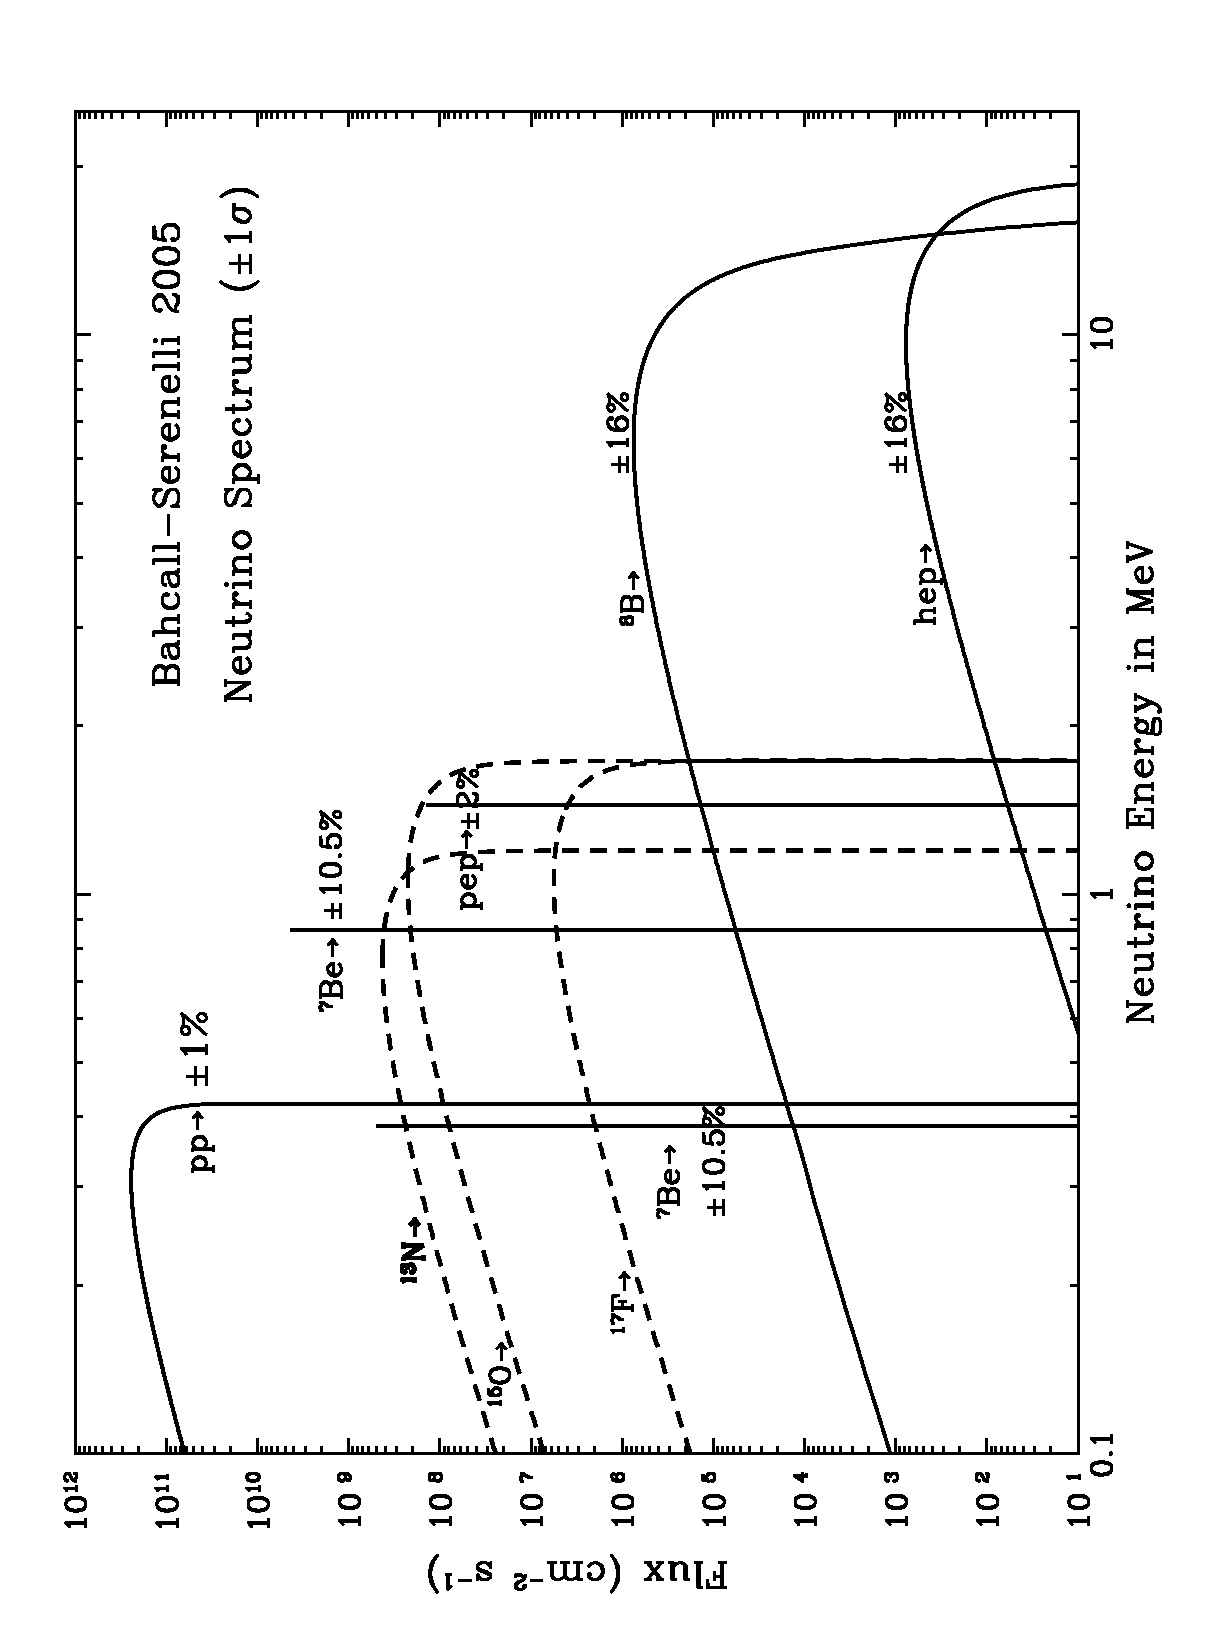
\includegraphics[angle=-90,origin=c,width=0.8\columnwidth]{bachall_bs05op}
\caption{\label{neutrino_spectra}Shown here are the fluxes and spectra of solar neutrinos as calculated in~\cite{bs05op}.
Solid lines show the proton-proton chain neutrinos, while dashed lines show the CNO cycle neutrinos.}
\end{figure}

\subsection{Standard Solar Models}

The fluxes shown in \Cref{neutrino_spectra} are from a theoretical calculation of the equilibrium state of the Sun known as a Standard Solar Model (SSM).
These calculations use hydrodynamic equations of state, contemporary solar observations, and estimations of the primordial composition of the solar system to infer the properties of the solar core.
These properties, such as temperature, density, and isotope content, directly control the rates of the various fusion reactions, and therefore predict the fluxes of solar neutrinos.
These rates depend strongly on predictions for nuclear cross sections at densities and temperatures consistent with the solar core, and uncertainties here drive the uncertainties in the neutrino fluxes.

\subsection{The MSW Effect}

The MSW~\cite{wolfenstein,mikheyev} effect proposes that the coherent forward scattering of electron flavor neutrinos off of electrons in a material adds a potential energy, $V_e$, to electron flavor neutrinos, which depends on the local electron density, $n_e$:
\begin{equation}
V_e = \sqrt{2} G_F n_e.
\end{equation}
Written in the mass basis the Hamiltonian including this effect, $H_{MSW}$, then takes the form
\begin{equation}
H_{MSW} = H_{0} + U\begin{bmatrix}
V_e & 0 & 0 \\
0 & 0 & 0 \\
0 & 0 & 0
\end{bmatrix}U^\dagger.
\label{eq:msw}
\end{equation}
Notably the evolution of the states in the presence of matter is now much more complicated since the eigenstates now depend on the electron density.

It is useful to introduce the matter mass basis, $\ket{\nu_{mi}(V_e)}$, consisting of eigenstates of the Hamiltonian $H_{MSW}$ at a particular electron potential $V_e$.
Note that if the electron density is zero, $H_{MSW}$ reduces to $H_0$. Therefore, $\ket{\nu_{mi}(0)} \rightarrow \ket{\nu_{i}}$.
In many cases the variation of $V_e$ is slow enough that the evolution is adiabatic, meaning some state $\ket{\nu(t)}$ has a constant probability to be one of the instantaneous matter mass states at a later time. 
\begin{equation}
\left| \braket{\nu_{mi}(V_e(0))}{\nu(0)} \right|^2 = \left| \braket{\nu_{mi}(V_e(t))}{\nu(t)} \right |^2
\end{equation}

The electron density within the sun varies sufficiently slowly for an adiabatic approximation to be made.
Therefore, knowing where in the Sun a neutrino is produced (or more precisely the electron density at the production point), one can calculate the eigenstate composition for as long as the adiabatic condition is satisfied.
Once the neutrino reaches the solar radius, vacuum propagation dominates. 
As vacuum propagation does not change the mass state composition of a state, the neutrinos that arrive at Earth have the same mass state composition as those exiting the Sun.
Due to the large distance between the Earth and the Sun, these mass state fluxes can be assumed to be incoherent once they arrive at Earth, and any regeneration of coherence in the Earth is ignored.
Regeneration of coherence while neutrinos propagate through matter is predicted by the MSW effect, and experiments have searched for this by measuring the asymmetry between neutrino fluxes during the night and day (when the neutrinos propagate through the Earth or not).
To date, this regeneration has not been observed to high significance, but the latest results from Super-Kamiokande show a small asymmetry at a bit over two sigma significance~\cite{superkiv}.
Therefore, the arrival probability $\phi_i$ of neutrino mass state $\nu_i$ at Earth due to electron neutrinos produced at an electron potential $V_e$ in the Sun in the presence of the MSW effect can be calculated as
\begin{equation}
\phi_i = \left| \braket{\nu_{m i}(V_e)}{\nu_e} \right|^2.
\label{rawflux}
\end{equation}
The analytic expression for this value is non-trivial and in practice $H_{MSW}$ is numerically diagonalized in the flavor basis to find $\bra{\nu_{m i}(V_e)}$ at a particular $V_e$ value and compute this projection.

Ultimately the MSW effect is the leading order effect responsible for the observed survival probabilities of solar neutrinos.
These expressions give the probability of electron neutrinos from the Sun interacting elsewhere as electron neutrinos, $P_{ee}$, or as another flavor neutrino, $P_{ea}$:
\begin{equation}
\begin{array}{rcl}
P_{ee} & = & \sum_i \phi_i |U_{ie}|^2  \\
P_{ea} & = & \sum_i \phi_i |U_{i\mu}|^2 + \phi_i |U_{i\tau}|^2
\end{array}
\label{msw_survive}
\end{equation}

For $^8$B neutrino energies in particular, the MSW effect is very important with $\phi_1 \approx \phi_3 \approx 0$, and $\phi_2 \approx 1$ meaning this flux is a quite pure sample of $\nu_2$ neutrinos. 
Lower energy solar neutrinos are not so affected, leading to dynamics closer to vacuum with $\ket{\nu_{mi}(V_e)} \approx \ket{\nu_i}$.
\Cref{fig:global_solar} shows all the solar neutrino flux measurements made to date overlaying the MSW survival probability.
With the leading order effects now understood, the door is open for precision measurements of neutrino, and, in particular, solar neutrino interactions.

\begin{figure}
\centering
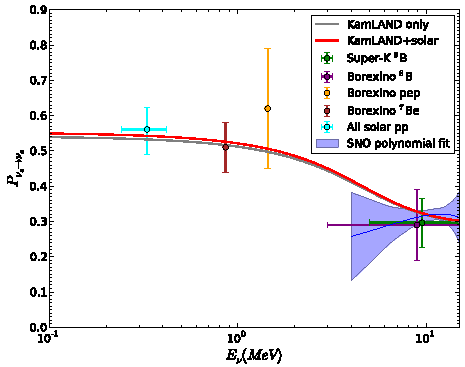
\includegraphics[width=0.8\columnwidth]{all_solar}
\caption{\label{fig:global_solar}Shown here are the measured fluxs of solar neutrinos at various energies by many solar experiments to date as given in~\cite{nonstandard_interactions}.}
\end{figure}

\subsection{Open Questions}
The solid lines in \Cref{fig:global_solar} represent the best fit MSW survival probability $P_{ee}$ as determined by combining the measurements of many solar neutrino experiments.
Notably, the error bars on the measurements, from which the best fits are derived, are quite large, leading to considerable uncertainty in the precise shape of $P_{ee}$.
This is of interest because new and interesting physics, such as nonstandard neutrino interactions with matter, would result in distortions to the survival probabilities, which would be measurable by solar neutrino experiments.
Here, ``nonstandard interactions'' are any sort of interaction not predicted by the Standard Model that somehow distinguishes between neutrino flavors, and hence influences the propagation of neutrinos in matter.
Much like the MSW effect, the influence from nonstandard interactions would be small, except for the very high densities present in the Sun, making solar neutrinos a viable probe of such effects.
The transition region between vacuum-dominated dynamics below 1~MeV to matter-dominated dynamics above 10~MeV is particularly sensitive to nonstandard interaction, however, this region has not yet been accurately probed by solar neutrino experiments.

To consider a specific possibility, nonstandard forward scattering~\cite{nonstandard_forward_scatter} of neutrinos off of fermions is a proposed effect similar to the MSW effect (standard forward scattering of electron neutrinos off of electrons).
Compared to the MSW Hamiltonian given in \Cref{eq:msw}, the Hamiltonian for nonstandard forward scattering allows for all neutrino flavors to couple to matter:
\begin{equation}
H_{NFS} = H_{0} + \sqrt{2} G_F n_e U\begin{bmatrix}
1+\epsilon_{ee} & \epsilon_{e\mu}^* & \epsilon_{e\tau}^* \\
\epsilon_{\mu e} & \epsilon_{\mu\mu} & \epsilon_{\mu\tau}^* \\
\epsilon_{\tau e} & \epsilon_{\tau\mu} & \epsilon_{\tau\tau}
\end{bmatrix}U^\dagger.
\label{eq:nsi}
\end{equation}
where the $\epsilon$ parameters represent the strength of the couplings.
This can be treated in an analogous way to the MSW effect to produce survival probability curves, of which examples can be seen in \Cref{fig:nonstandard}.
Such models cannot be disentangled from the standard MSW effect until higher precision measurements of the survival probability exist in this transition region.

\begin{figure}
\centering
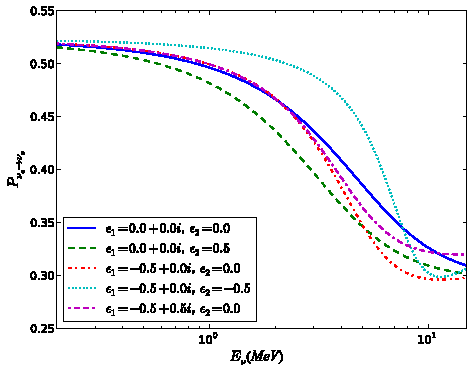
\includegraphics[width=0.8\columnwidth]{nonstandard_interactions}
\caption{\label{fig:nonstandard}Shown here are predictions of the survival probability from nonstandard neutrino forward scattering which cannot be disentangled from the standard MSW effect with existing solar neutrino measurements. The $\epsilon_1$ and $\epsilon_2$ parameter are analogous to the parameters in \Cref{eq:nsi}, but for a two neutrino scenario. Figure from~\cite{nonstandard_interactions}.}
\end{figure}

Another possibility, since it is now known that neutrinos are massive particles, is that neutrino mass states could decay to some lighter states.
This can also be treated as a distortion to the survival probabilities, since the signature of neutrino decay is a disappearance (non-detection) of neutrino flux.
An analysis seeking to measure the effect of neutrino decay is discussed further in \Cref{ch:lifetime}, where distortion to the survival probability indicative of neutrino decay is used to set a limit on neutrino lifetime.

Further, the rate of the CNO process in the Sun, which is proportional to the CNO neutrino fluxes, is currently only constrained by analyses done by Borexino.
A high precision measurement of the CNO neutrino flux will provide information about the abundance of elements heavier than helium (``metallicity'') in the core of the Sun that are necessary for the CNO process.
At the moment there is tension between standard solar model predictions of metallicity and spectroscopic measurements done of the surface of the Sun, and a better understanding of the CNO neutrino fluxes could resolve some of this tension.
A measurement of the CNO neutrinos is a goal of current and next-generation solar neutrino detectors, however, their low energies and a similarity to the energy spectrum of radioactive contaminates makes this quite difficult.

\clearpage

\chapter{Solar Neutrino Detectors}
\label{ch:detectors}

Neutrinos only interact weakly with normal matter, so the interaction cross sections are quite small, being less than $10^{-40}$~cm$^2$ for energies relevant to solar neutrinos.
Even with expected fluxes of detectable solar neutrinos exceeding $10^6$~cm$^{-2}$s$^{-1}$, the interaction rates are minuscule.
Because of this, neutrino detectors typically rely on large masses of target material to achieve a reasonable interaction rate, with a solar neutrino event a day being quite respectable.
These low rates mean that neutrino detectors must be isolated from cosmic radiation by being constructed deep underground, or lose the neutrino events in the noise.
Even then the materials used to construct the detector must have very low intrinsic radioactivity or suffer the same fate.

\section{Radiochemical Experiments}

The earliest neutrino detectors relied on the transmutation of nuclei by neutrino interactions. 
In the Homestake~\cite{homestake} experiment, chlorine nuclei were transformed to argon nuclei via a neutrino capture,
\begin{equation}
\nu_e + ^{37}\mathrm{Cl} \rightarrow ^{37}\mathrm{Ar} + e^-,
\end{equation}
and the created argon was periodically collected its decays counted to estimate the interaction rate in the target volume.
The gallium experiments GNO~\cite{gno}, GALLEX~\cite{gallex}, and SAGE~\cite{sagecombo}, relied on a similar method with gallium:
\begin{equation}
\nu_e + ^{71}\mathrm{Ga} \rightarrow ^{71}\mathrm{Ge} + e^-.
\end{equation}
Notably detectors relying on these radiochemical methods were only sensitive to $\nu_e$ and the solar neutrinos that had oscillated into another flavor were not detected, resulting in the SNP.
Also of note is that these detectors individually provide no information about the neutrinos besides the interaction rate above the minimum energy threshold necessary to transmute the isotope used in the detector. 
Some spectral information can be obtained by looking at results from different isotopes with different minimum energy thresholds, however, event-by-event neutrino energy and direction information is totally lost in the radiochemical detection scheme.

\section{Real-Time Neutrino Detection}

The next generation of neutrino detectors progressed to real-time detection of neutrino interactions.
These were the water Cherenkov detectors, the most recent of which include SNO~\cite{3phase} and Super-Kamiokande~\cite{superk}, which instrumented a large volume of water with sensitive light detectors that captured flashes of Cherenkov light from energetic particles produced in the neutrino interaction.
Pure water detectors, like Super-Kamiokande, detect neutrinos through the elastic scatter interaction,
\begin{equation}
\nu_e + e^- \rightarrow \nu_e + e^-,
\end{equation}
where the final state electron has a momentum highly correlated with the incident neutrino.

Real-time detectors measure properties about each neutrino interaction as they occur instead of simply counting the number of interactions that happened within a given amount of time.
Analysis of data collected by real-time detectors allows for a statistical determination of the properties of the neutrino flux that produced such interactions.
Real-time detection also allows for different interaction channels to be distinguished, a feature leveraged by the SNO detector, which was instrumental in solving the SNP.

From water Cherenkov detectors, the field has progressed to target media other than water, such as the use of liquid scintillators in Borexino~\cite{borexino} and KamLAND~\cite{kamland}, which can provide complementary information and lower energy thresholds compared to water.
As this progression is an important theme in this thesis, the following sections go into some details about the merits of each.

\subsection{Cherenkov Radiation}

Ultimately all light from physics interactions detected in water Cherenkov detectors was the result of electrons being scattered with sufficient energy to exceed the local speed of light, commonly called Cherenkov radiation~\cite{cherenkov}.
This light is emitted at an angle relative to the direction of the particle track, which depends on the index of refraction of the material.
Because of this, the geometry of the detected hits from Cherenkov radiation can be used to infer the average direction of the electron with resolution of order 10 degrees.
In the cases of ES events, where the electron direction is highly correlated to the primary neutrino direction, this information can be used to disentangle solar neutrino events from backgrounds.
This was leveraged in analyses of SNO data and is a very beneficial feature when dealing with directional sources.

\subsection{Scintillation Light}

As a charged particle moves through a scintillator, electronic energy levels in the scintillator are excited, which can subsequently relax by emitting a visible photon.
In the case of {\labppo} in {\snop}, this results in roughly ten thousand scintillation photons per MeV compared to hundreds of Cherenkov photons.
The much larger number of photons results in much better energy resolution \textit{c.f.} a water detector, which is very advantageous to analyses that rely heavily on energy reconstruction.

Unlike Cherenkov light, scintillation light is emitted isotropically, since the relaxing of the vibrational state is uncorrelated with the direction of the incident particle.
Further, scintillators are optically less transparent than water (typically) leading to increased scatter (isotropy) in the emitted light.
With much of the Cherenkov light scattered by the scintillator, and the remaining Cherenkov photons buried under two orders of magnitude more scintillation photons, there are very few remaining Cherenkov photons carrying directional information, and those that remain are hard to identify among the scintillation photons.
This leads to the significant downside of being unable to reliably reconstruct direction and, therefore, being unable to disentangle events based on directionality. 
For solar neutrinos this is a significant loss, because typically there is no other class of events correlated with the direction of the sun.
This is applicable both in analyses where solar neutrinos are of interest and should be selected, and also where solar neutrinos would be considered a background and should be rejected.

The final significant difference between Cherenkov and scintillation light is the minimum energy threshold.
Cherenkov light relies on the charged particle being very relativistic (exceeding the local speed of light), meaning that $\alpha$ particles are typically invisible, while betas must exceed 0.7 MeV total energy, to emit any light.
Scintillation, on the other hand, only has the constraint that sufficient energy be deposited to excite vibrational states, typically on the order of eV.
In the case of scintillation, both alphas and betas from radioactive decays are visible, since both can deposit sufficient energy to create scintillation light.
In scintillator detectors, therefore, the maximum rate of the detector electronics are the limiting factor for data acquisition, not the interaction threshold of the medium.
For solar neutrinos, the capability to see lower energy interactions gives access to virtually all types of neutrino fluxes, not just the $^8$B neutrinos accessible by water Cherenkov detectors.
The Borexino~\cite{borexino} and KamLAND~\cite{kamland} experiments have made excellent solar neutrino measurements with scintillator, and {\snop} plans similar analyses for scintillator phase.

\subsection{Combined Scintillation and Cherenkov Signal}

There are multiple technologies in development with the goal of having simultaneously detectable Cherenkov and scintillation signals, however, for this thesis I will focus on one in particular: water-based liquid scintillators (WbLS).
WbLS mixes a traditional scintillator, {\labppo}, an oil, with water at some configurable ratio that is in large part water.
In principle the fraction of scintillator results in a fraction of total light output from a pure scintillator, so low scintillator fractions will have a comparable number of scintillation photons to Cherenkov photons. 
This leads to enhanced energy resolution compared to only Cherenkov light, while allowing for the possibility of observing Cherenkov geometry in the pattern of detected photons, and thereby obtaining direction information.
At higher scintillation fractions, the relatively fewer Cherenkov photons might be difficult to identify on top of the isotropic scintillation light.
In this case one may leverage the fact that Cherenkov light is very prompt (picoseconds) compared to scintillators ({\labppo} has a short time constant of a few nanoseconds) to potentially identify Cherenkov photons as the most prompt hits.
Finally, being mostly water, WbLS should have longer scattering and attenuation lengths than a pure scintillator, allowing larger volumes to be built before either effect becomes a limiting factor.
This seems to identify WbLS as an ideal material for combining the long attenuation lengths of water with the directionality of Cherenkov light and higher energy resolutions of scintillating materials.
Further discussion of WbLS and a characterization of low scintillator fractions can be found in \Cref{ch:wbls}.

\section{SNO}

\begin{figure}
\centering
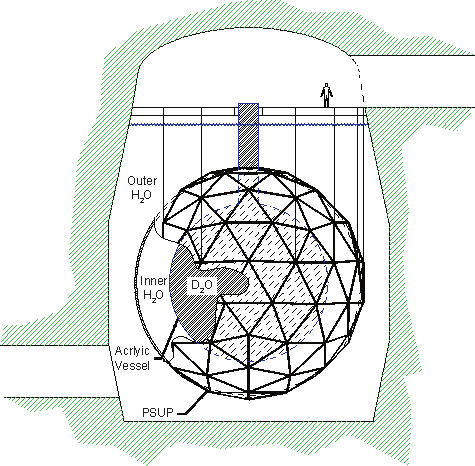
\includegraphics[width=0.8\columnwidth]{sno}
\caption{\label{fig:sno}The SNO detector as shown in~\cite{3phase}.}
\end{figure}

The SNO~\cite{sno} detector is located deep underground near Sudbury, Canada in the Creighton mine, an active nickle mine.
This location is one of the deepest laboratories in the world at $2$~km underground, providing a 5800 m.w.e. overburden to shield from cosmic rays.
The detector itself is composed of a 6-m radius acrylic vessel (AV) in the shape of a spherical shell containing 1 kT of heavy water ($^2$H$_2$O or D$_2$O) as the active volume.
Heavy water was chosen because the loosely bound neutron in the deuterons enabled both neutral current and charged current interactions enabling flavor selective measurements of the solar neutrino flux.

\subsection{Neutrino Detection}

As in other water Cherenkov detectors, SNO is sensitive to the elastic scatter (ES) of neutrinos off electrons in the water as shown in \Cref{fig:ES}.
For electron neutrinos, both W and Z bosons can be exchanged.
However, solar neutrinos do not have enough energy to produce heavier leptons, so only Z exchange is possible for non-electron flavor neutrinos.
This means the ES interaction is sensitive to all flavors of neutrino, but with non-electron flavor neutrinos having a lower cross section.
Due to kinematics, the final direction of the scattered electron is highly correlated with the initial direction of the neutrino.
However, the energy is shared between the outgoing neutrino and scattered electron, meaning that the observed electron energy is only loosely correlated with the neutrino energy.
This means that ES interactions give poor spectral information, but very precise direction information.
For solar neutrinos, this means ES electrons will point away from the Sun.

\begin{figure}
\centering
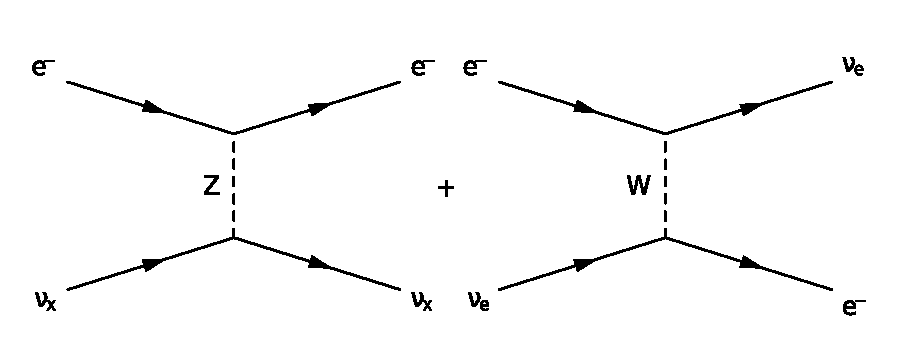
\includegraphics[width=\columnwidth]{feyn_es}
\caption{\label{fig:ES}The Feynman diagrams for elastic scatter (ES) interactions with electrons. 
Note that all neutrino flavors can exchange a Z boson, but only electron flavor neutrinos can exchange a W boson.}
\end{figure}

The deuterium in the heavy water target used in SNO allows two other types of interaction, each sensitive to different combinations of neutrino flavors.
Most important is the neutral current interaction (NC) due to a neutrino scattering off a quark, as shown in \Cref{fig:NC}.
NC is equally sensitive to all flavor of neutrino, allowing for an oscillation-agnostic measure of the total neutrino flux.
In practice the energy deposited in the quark results in a detectable signal if it exceeds the binding energy of the proton and neutron forming a deuteron.
The liberated neutron will eventually capture on some nuclei, resulting in a cascade of gammas, which can scatter electrons with sufficient energy to produce Cherenkov light.
Due to the detection scheme, information about the energy and direction of the initial neutrino is lost in NC interactions.

\begin{figure}
\centering
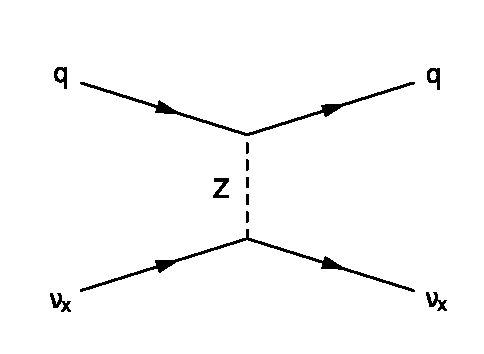
\includegraphics[width=0.6\columnwidth]{feyn_nc}
\caption{\label{fig:NC}The Feynman diagram for neutral current (NC) interactions with quarks.}
\end{figure}

Neutrinos can undergo a charged current (CC) interaction with quarks in a deuteron, shown in \Cref{fig:CC}.
The CC interaction converts the neutron into a proton, breaking up the deuteron, and producing an energetic electron with an energy correlated to the incident neutrino energy.
In principle any neutrino flavor could participate in a CC interaction, however, solar neutrinos do not have sufficient energy to create heavier leptons.
Muon and tau flavor neutrinos, therefore, cannot exchange a W boson, and do not participate.
The energetic electron then produces Cherenkov light to be detected.
This interaction channel allows for the recovery of spectral information due to the correlation of the electron energy to the neutrino, and provides an exclusive measurement of the electron-neutrino flux. 


The ratio of CC to NC interactions can directly give the average electron neutrino survival probability.
The NC interaction represents a flavor agnostic measurement of the neutrino flux, while the CC interaction is exclusive to electron neutrinos.
This ratio of the two is precisely the definition of $P_{ee}$: the fraction of solar neutrinos detected as electron flavor neutrinos.

\begin{figure}
\centering
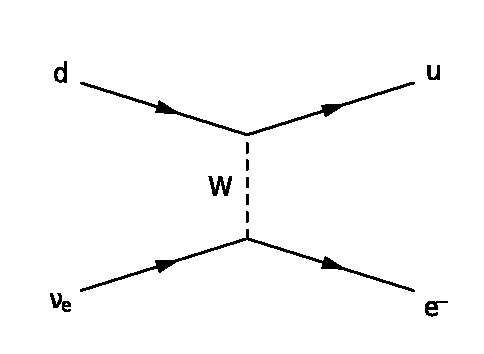
\includegraphics[width=0.6\columnwidth]{feyn_cc}
\caption{\label{fig:CC}The Feynman diagram for charged current (CC) interactions with quarks.}
\end{figure}

\subsection{Experimental Phases}

SNO operated in three distinct phases differing in their neutron detection capabilities, and hence their sensitivity to the NC interaction.
This was achieved by modifying the target material between phases of data taking.
These phases are described in the following sections along with the neutron detection mode in each phase.

\subsubsection{Phase I}

The first phase consisted of a pure D$_2$O target. 
Neutrons produced in the NC interaction primarily captured on other deuterons in the target.
The produced $^3$H then decayed, releasing a 6.26-MeV gamma.
This gamma could either scatter electrons in the target or create energetic electron-positron pairs, either mode being detected by Cherenkov light.

\subsubsection{Phase II}

In the second phase, NaCl was added to the D$_2$O target.
Chlorine has a much greater neutron capture cross section than deuterium, resulting in a significant increase in neutron detection efficiency.
The decay scheme after a neutron capture on Cl is quite complicated, releasing many gammas, and giving these events a more isotropic topology compared to other interactions.
Neutron detection was further enhanced by an increase in total energy released in the gamma cascade to 8.6 MeV.

\subsubsection{Phase III}

Finally, in the third phase, the NaCl was removed from the target, and neutron counting devices (NCDs) were added inside the AV.
These were essentially independent detectors, allowing for an independent measure of the neutron production rate.
A single NCD was a high purity nickel tube containing $^3$He gas, and was instrumented to utilize the $^3$He as a proportional counter for thermal neutrons~\cite{sno_ncd_psa}.
In total, 40 NCDs were added, two of which were modified to contain $^4$He (insensitive to neutrons) to understand instrumental backgrounds.
The NCD data is not directly used in the analysis described in the next chapter, however, it was independently analyzed to constrain the analysis of the PMT data~\cite{3phase}.

\subsection{Detector Design}

The target material is contained within a 6-m radius AV.
The AV is surrounded by a 9-m radius steel geodesic structure, containing 9500 inward-facing photomultiplier tubes (PMTs), called the PMT support structure (PSUP).
These PMTs are sensitive to single photons and are intended to capture the Cherenkov radiation from energetic charged particles within the AV.
The entire structure is submerged in a large barrel shaped cavity of light water (H$_2$O) to shield the heavy water in the AV from the natural radioactivity of the mine and other detector materials.
Both the heavy water inside the AV and the light water of the cavity were continually purified to keep intrinsic radioactivity low and cooled to minimize biological growth.

The PMTs used in SNO were 8-inch Hamamatsu R1408 created with low-radioactivity glass. 
These PMTs had a time resolution for detected photons of 1.5~ns, and a peak quantum efficiency of 21.5\% at 440~nm.
Each PMT was outfitted with non-imaging light-concentrating reflectors to increase the effective coverage of light-sensitive elements to 55\%.
To assist in vetoing cosmic rays, 91 additional PMTs were mounted to the PSUP looking outward into the light water of the cavity. 

Whenever a PMT detected a photon, a discriminator would fire on the corresponding voltage fluctuation and register a hit.
This hit started a voltage ramp on a time-to-amplitude converter (TAC) to track the hit time, and integrated the total charge collected by the PMT.
Additionally, the PMT readout electronics would emit two  10-mV square pulses of configurable widths, which are summed across the entire detector and act as a count of coincidentally hit PMTs within each window.
For SNO these windows were set to approximately 20~ns and 100~ns.
The trigger system discriminated the analog sum of each trigger, and, when it crossed a configurable threshold, the trigger system would issue a global trigger (GT) causing all PMTs hit in the last 400~ns to report the value of their TAC (representing the time before the global trigger) and integrated charge (representing the number of detected photons --- typically one).
For SNO the discriminator threshold on trigger sums corresponded roughly to 17 hit PMTs.
The hits from each GT are built into a single event for further analysis.

\subsection{Vertex Reconstruction}

To perform an analysis of SNO data it is first necessary to extract physical observables from the PMT hit time information provided by the DAQ.
This is done using pattern recognition algorithms, which take into account the geometry of Cherenkov light to reconstruct the direction, position, and time of each event.
Using that information, along with the total number of hits, other algorithms can estimate the energy deposited in the detector. 
Further quantities can be extracted, such as a measure of the isotropy of the event and the ratio of hits within a prompt time window to all hits, encode additional information about the event that can, for instance, be useful for selecting physics events from instrumental events.
Cherenkov light has a very specific geometry, so good physics events will have a characteristic spatial distribution of detected photons, allowing isotropy to be used to cut instrumental backgrounds.
Similarly, Cherenkov light is very prompt, meaning all photons from a physics event are expected to arrive within tens of nanoseconds, and making the ratio of in-time hits a useful metric for identifying candidate physics events. 

\subsection{Calibration}

To understand detector response and characterize the algorithms that perform the vertex reconstruction, sources with known energy spectra or well-defined photon emission times that can be deployed at known positions within the detector are critical.
Two sources were critical in this effort:
\begin{description}
\item[\N~\cite{sno_n16}] This isotope is produced with a deuterium-tritium neutron generator by captures on $^{16}$O producing $^{17}$O, which quickly decays by emitting a proton to leave \N. This isotope is transported in gas form to a calibration source within the detector where it beta decays into a metastable state of $^{16}$O that relaxes, releasing a 6.13-MeV gamma. The initial beta decay provides a tag signal within the source, and the gamma escapes into the detector where it deposits its energy. This source provides the energy scale calibration for SNO by calibrating its photon detection efficiency. It is also used to evaluate energy and position reconstruction systematics as a function of position within the detector and throughout the operational time of the detector.
\item[Laser Ball~\cite{sno_laserball}] A fast dye laser is fiber coupled to an optical diffuser, which work together to produce an isotropic light pulse at a well-defined time. This is primarily used to calibrate the time offset of each PMT, and can also be used to measure relative detection efficiencies of the PMTs.
\end{description}
Additional sources were used to provide calibration points at other energies, such as a beta source using \Li~\cite{Tagg:2002} with an endpoint at 14~MeV, and a proton fusion source~\cite{fusion_source} producing a gamma at 19.8~MeV.
Sources producing the decay chains of $^{238}$U and $^{232}$Th were deployed for low energy calibrations.
Additionally, the heavy water target was at times intentionally spiked with both radon and $^{24}$Na to provide calibrations unbiased by the presence of shielding that is unavoidable in encapsulated sources.
Finally, to characterize the neutron detection efficiency critical for the measurement of the NC interaction, two neutron sources were deployed: $^{252}$Cf and an AmBe source.

The deployed sources were lowered into the detector through the neck via the manipulator system.
This used a central umbilical to provide power or gas-transport to the sources, and additionally used a rope system to accurately position the sources within the detector volume.

\subsection{Previous Results}

As mentioned, SNO was instrumental in demonstrating flavor change of solar neutrinos, and this was possible by using the flavor discrimination of the available interaction channels.
By using the distinct signatures of NC, CC, and ES events, SNO was able to measure the rates of each type of interaction.
These rates could be converted into incident neutrino fluxes, $\Phi_{NC}$, $\Phi_{CC}$, and $\Phi_{ES}$, by unfolding the detector response and interaction cross sections (with assumptions about the spectral shape of $^8$B neutrinos).
Then knowledge of the flavor discrimination of each interaction channel allows constraints on these fluxes to be constraints on the flavor components, $\Phi_e$ for electron flavor and $\Phi_{\mu\tau}$ for muon and tau flavor, of the overall neutrino flux:
\begin{equation}
\begin{split}
\Phi_{NC} &= \Phi_{e} + \Phi_{\mu\tau} \\
\Phi_{CC} &= \Phi_{e} \\
\Phi_{ES} &= \Phi_{e} + \epsilon \Phi_{\mu\tau} \\
\end{split}
\end{equation}
where $\epsilon$ represents the relative interaction cross section for electron and other flavor neutrinos.
Graphically this is shown in \Cref{fig:sno_flavor}, which conclusively demonstrates a non-electron flavor component to the total neutrino flux.

\begin{figure}
\centering
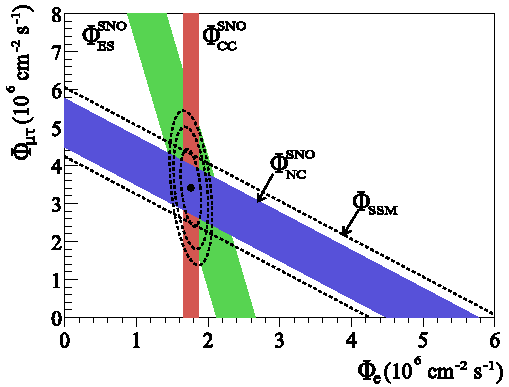
\includegraphics[width=0.8\columnwidth]{sno_flavor}
\caption{\label{fig:sno_flavor} Direct evidence for flavor change in solar neutrinos from SNO taken from~\cite{sno_direct}.}
\end{figure}

Later SNO analyses, such as the Low Energy Threshold Analysis (LETA)~\cite{leta} of Phases I and II of SNO data, or the extension of this including Phase III data, aptly referred to as the 3-phase analysis~\cite{3phase}, were able to fit directly for the survival probability $P_{ee}$ as a function of neutrino energy.
Since neutrino energy is not something SNO observed directly (the ES and NC interactions give little to no spectral information), a method was developed to determine the impact of $P_{ee}$ on observable quantities.
Since $P_{ee}$ can be taken as the fraction of neutrinos that are electron flavor as a function of energy, weighting the $^8$B energy spectrum used to describe $\Phi_e$ properly accounts for the energy dependence of $\nu_e$ survival.
In the same way, the $^8$B energy spectrum for $\Phi_{\mu\tau}$ may be weighted by $1-P_{ee}$ to account for the neutrinos converted to $\nu_\mu$ or $\nu_\tau$.
To making assumptions about the shape of the survival probability, SNO opted to parameterize $P_{ee}$ by a second degree polynomial.
The result of this style of analysis can be seen in the earlier \Cref{fig:global_solar}.
By comparing the fitted survival probability to models of neutrino propagation, most notably the MSW model described earlier, SNO was able to constrain neutrino oscillation parameters.
Building off this style of analysis one is able to probe neutrino physics as a function of neutrino energy and investigate other effects beyond MSW that would influence neutrino propagation.

\section{\texorpdfstring{\snop}{SNO+}}

The SNO experiment finished taking data in the early 2000s, and an upgrade of the detector was planned, which ultimately led to {\snop}~\cite{snop}.
The primary goal of {\snop} is a measurement of neutrinoless double beta decay, which, if observed, would shed light on whether the neutrino is its own antiparticle and on the nature of neutrino mass.
Also included in the goals of {\snop}, and of particular relevance to this thesis, is a measurement of lower energy solar neutrino fluxes, particularly the CNO neutrinos, enabled by a switch of target mediums to a scintillating liquid also necessary for neutrinoless double beta decay sensitivity.
To enable this change in targets, some modifications to the experiment were necessary: the detector electronics required upgrades to handle the higher data rate expected with lower energy thresholds, and the AV required the installation of hold-down ropes since scintillator has a lower density than water and would otherwise tend to float in the water shield.
A rendering of the upgraded detector can be seen in \Cref{fig:snop}.
Additionally, the chemical plants to purify and process scintillator, and other supporting hardware, needed to be installed underground, which was no small task.

\begin{figure}
\centering
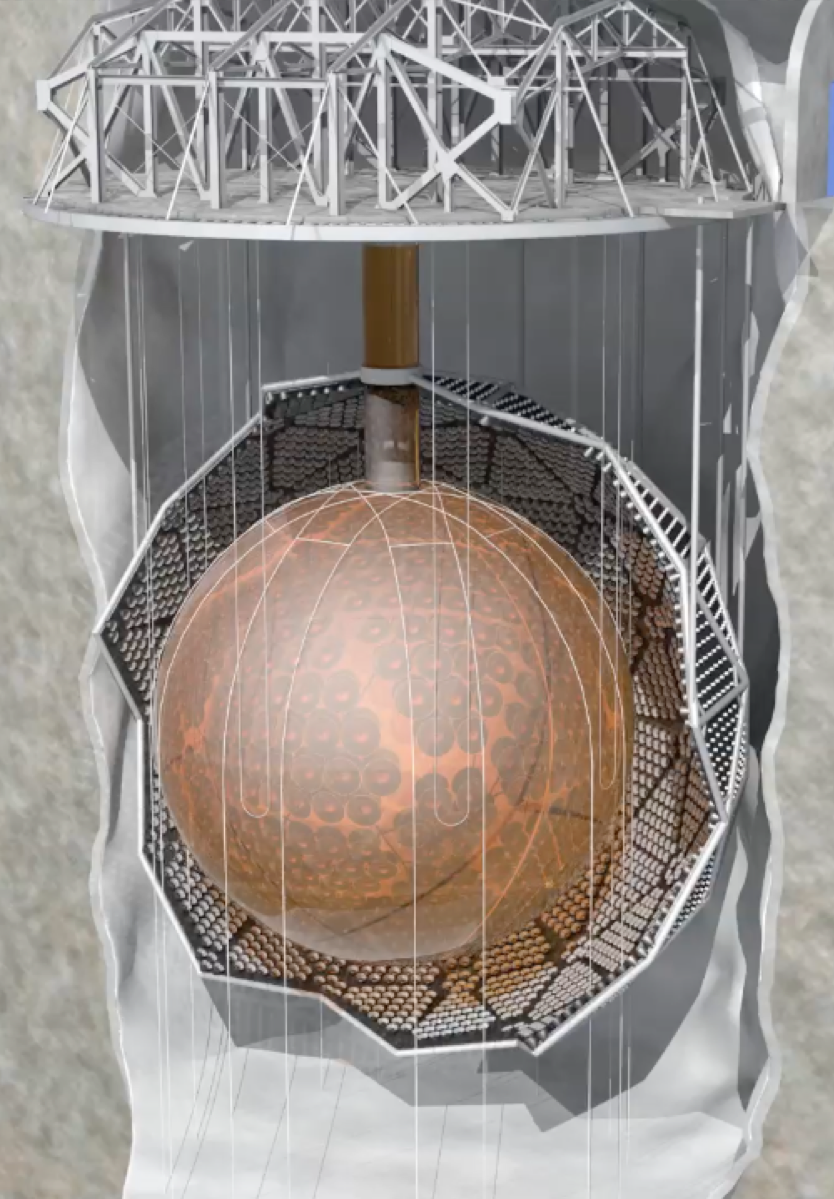
\includegraphics[width=0.5\columnwidth]{snop.png}
\caption{\label{fig:snop}A rendering of the {\snop} detector. Note the PSUP is only partially rendered to expose the AV contained within.}
\end{figure}

\subsection{Experimental Phases}
Similar to SNO, {\snop} intends to operate in three experimental phases.
The first phase is of primary relevance to this thesis, however, all three are described in the following sections.

\subsubsection{Light Water}
Water phase in {\snop} is intended to calibrate the detector and test the upgraded hardware in a regime similar to SNO, while also generating physics data as a deep underground water Cherenkov detector.
As part of the calibration effort in water phase, \Cref{ch:chsrc} describes an optical calibration source designed for {\snop}, which will be calibrated in water phase and then used to calibrate later phases of the experiment.
Of physics interest in this phase are a search for nucleon decay~\cite{nucleon_decay}, potential sensitivity to anti-neutrinos in pure water, and the elastic scatter of solar neutrinos.
Relative to other water Cherenkov detectors, SNO benefits from its deeper location in a reduced muon flux, and hence reduced cosmogenic backgrounds
In terms of solar neutrinos, light water differs from heavy water primarily in the available interaction channels: neither NC nor CC are possible given the lack of targets (deuterons) with sufficiently low interaction thresholds.
The ES interaction is unaffected by this change in targets, since both H$_2$O and D$_2$O have roughly the same electron density.
\Cref{ch:es} goes into detail on measuring the $^8$B solar neutrino flux in {\snop} with the ES channel.
Data taking for this phase began mid 2017 and finished toward the end of 2018.

\subsubsection{Scintillator}

The change to pure scintillator {\labppo} (linear alkylbenzene with a primary flour 2,5-diphenyloxazole at 2~g/L) started at the end of 2018 with the gradual displacement of water inside the AV.
This switch was motivated by a need for enhanced energy resolution for the neutrinoless double beta decay measurement, and similar reasoning comes into play in its applicability to solar neutrinos.
In terms of solar neutrinos, the ES interaction channel is still the only relevant one, however, the observed signals in scintillator phase will be quite different from that of water phase.
In water all information about the interaction was gathered from the Cherenkov light emitted. 
Cherenkov light will still be generated in scintillator, however, in {\labppo} it will be insignificant compared to the light emitted by the relaxing of vibrational states of the scintillating medium itself.
As of the writing of this thesis, scintillator phase is moving forward, but physics data taking is still in the future.

\subsubsection{Tellurium Loaded Scintillator}
As mentioned, the primary goal of {\snop} is to perform a neutrinoless double beta decay measurement using the double beta decay isotope $^{130}$Te.
This will be done by dissolving $^{130}$Te metal in the {\labppo} scintillator, and searching for an excess of events at the endpoint ($Q \approx 2.6$~MeV) of $^{130}$Te decay.
The basic principle behind this measurement is that a double beta decay with neutrinos should follow a double beta decay energy spectrum, where some fraction of the decay energy is not observed due to being carried away by neutrinos, while a neutrinoless decay would deposit the entire decay energy into the electrons, resulting in a delta function spectrum at the endpoint.
Since the signature of this process is a sharp feature in energy, {\snop} requires the enhanced energy resolution of scintillators, as such a measurement would not be possible with the energy resolution of Cherenkov light.

\subsection{Calibration}

{\snop} makes extensive use of SNO calibration hardware in its calibration effort, however, upgrades of the deployment hardware are planned for scintillator phase to meet the more stringent background requirements of that phase.
For water phase, both the SNO \N and Laser Ball sources were used in the same manner as in SNO.
An upgrade of the SNO Laser Ball is under construction for scintillator phase in {\snop}.
The timing calibration typically by the Laser Ball is intended to be replaced by a fast pulsed LED system called ELLIE, which is fiber coupled to known positions on the PSUP, and does not require deployment of a source into the target volume.
A new calibration source (described in \Cref{ch:chsrc}) intended to replace the \N calibration of photon detection efficiency for scintillator phase was developed.
Finally, new radioactive sources, such as a $^{48}$Sc and $^{57}$Co, are being developed to assist in energy scale calibrations in tellurium loaded phase, while intrinsic radioactivity present in the scintillator provides another means for calibrating energy scale.

\section{\textsc{Theia}}

\textsc{Theia}~\cite{asdc_paper} is a proposed large scale (50-100~kT) neutrino detector, which aims to support a diverse platform of neutrino physics. 
Of particular relevance to this thesis is the goal of doing high precision measurements of solar neutrinos~\cite{theia_solar}.

\subsection{Conceptual Design}
The detector design is still in the conceptual phase, but lessons learned from {\snop} and other liquid scintillator detectors are being incorporated, and the optical detection scheme remains roughly unchanged except for potential upgrades to technologies similar to PMTs.
The basic plan is two-fold: build a very large detector to maximize interaction rate and enhance fiducial volume shielding, and develop a novel target medium that combines the advantages of Cherenkov and scintillation light.
The former is primarily an engineering and/or funding challenge, while the latter presents an interesting research topic that is explored further in \Cref{ch:wbls}.
The baseline design calls for a right cylinder around 40~m across filled with WbLS and surrounded with fast photodetectors.
The optical clarity of WbLS should allow scaling to these sizes without undue loss of photons to attenuation.

\subsection{Sensitivity to Solar Neutrinos}
With WbLS comes the possibility of simultaneously detecting a Cherenkov and scintillation signal.
The presence of a Cherenkov signal means that the direction reconstruction is again possible, while the scintillation light will enhance the energy resolution relative to water Cherenkov detectors, and allow for detection of events below the Cherenkov threshold.
In particular, simulations suggest \textsc{Theia} would have good sensitivity to the CNO cycle neutrinos~\cite{theia_solar}.

The WbLS in consideration for \textsc{Theia} would be primarily water, and this allows for easy loading of metals into the detector.
Of primary interest are isotopes like $^7$Li, which, like the deuterons in the heavy water in SNO, have low enough binding energies for solar neutrinos to participate in a CC interaction~\cite{asdc_paper}.
As the CC interaction has a visible energy much better correlated with the incident neutrino than the ES interaction, loading such an isotope in WbLS in \textsc{Theia} would enable high resolution measurements of the solar neutrino spectra. 




\chapter{Constraints on Neutrino Lifetime from SNO}
\label{ch:lifetime}

Analysis of the SNO data was instrumental in solving the SNP, and with the leading order dynamics of neutrinos established as the MSW effect, one can now explore the SNO data to constrain second order effects. 
Neutrino decay is one such effect, and was first explored as a possible explanation for the less-than-unity survival probability of electron flavor neutrinos~\cite{bachall_stable}.
Even though neutrino decay is now known not to be the dominant effect behind the SNP, solar neutrinos make an excellent test beam for investigating neutrino decay.
Roughly speaking, this analysis will be searching for a deficit of neutrinos resulting from decay of neutrinos in flight from the Sun to the Earth.
As will be shown in the following sections, this produces an energy dependent distortion to the MSW survival probability curves that can be fit for in an analysis of SNO data.

The initial proposal to use solar neutrinos as a handle on neutrino lifetime explored a few models of neutrino decay and estimated that solar neutrinos could put the best limit on non-radiative neutrino decay~\cite{beacombell}.
The authors noted that the large uncertainty on the $^8$B flux as well as uncertainties in the neutrino mass and mixing parameters would be a limiting factor.
Relatively recent precise mixing parameters from KamLAND~\cite{kamland} and Daya Bay~\cite{dayabay} and improved theoretical predictions for the $^8$B flux~\cite{serenelli} mitigate this to some extent.
Further studies~\cite{berryman} using a simple disappearance model - where the neutrino decays into some non-active daughter(s) and the observable signal is an energy dependent distortion to the survival probability - were able to set respectable limits analyzing SNO~\cite{sno}, Super-Kamiokande~\cite{superk}, and Borexino~\cite{borexino} results.
Various constraints such as the eccentricity of the Earth's orbit allowed this limit to be improved~\cite{picoreti}. 
However, it was noted~\cite{berryman} that the published fits to the SNO data were not ideal for testing the simple disappearance model because the survival probabilities for electron neutrinos, $P_{ee}$, and the transition probability to other neutrino flavors, $P_{ea}$, were not treated as independent functions.
In a decaying scenario these probabilities are modified by an energy dependent form that does not preserve $P_{ee} + P_{ea} = 1$, which is a valid assumption in non-decaying scenarios and used in previous SNO analyses, so the authors concluded a better limit could be set with a dedicated fit.
This analysis aims to perform such a dedicated fit, specifically for the $\nu_2$ lifetime observed as an energy dependent modification to the standard MSW survival probability.

\section{Lifetime Model}
\label{lifetime_model}

The flux of a particular mass state $\nu_i$ could have some lifetime associated with it $\tau_i$ representing the decay of neutrinos of that mass state.
Since the actual neutrino masses are unknown the lifetime is often represented by an effective parameter $k_i$ scaled by the mass of the state
\begin{equation}
k_i = \frac{\tau_i}{m_i}.
\end{equation}
Since the Earth-Sun distance is so large compared to the solar radius any decay within the sun will be ignored. 
Therefore, using the formalism given in \Cref{ch:theory}, the detected flux $\psi_i$ of a neutrino mass state at earth can be given as 
\begin{equation}
\psi_i \approx  e^{-L_\odot / (E k_i)} \phi_i =  e^{-L_\odot / (E k_i)} \left| \braket{\nu_{m i}(V_e)}{\nu_e} \right|^2
\label{decay}
\end{equation}
where $L_\odot$ is the Earth-Sun distance (1~A.U.) and $E$ is the neutrino energy.
The survival probabilities for electron and muon/tau flavor neutrinos in a decaying scenario may then be calculated with appropriate factors from the PMNS matrix in the usual way,
\begin{equation}
\begin{array}{rcl}
P_{ee} & = & \sum_i \psi_i |U_{ie}|^2  \\
P_{ea} & = & \sum_i \psi_i |U_{i\mu}|^2 + \psi_i |U_{i\tau}|^2.
\end{array}
\label{survive}
\end{equation}

\subsection{Computing Survival Probabilities for \texorpdfstring{$^8$B}{Boron-8} Neutrinos}

\label{montecarlo}

The three neutrino mass states each have a lifetime associated with them $k_i = \tau_i / m_i$, which are all physically interesting quantities to measure.
However, the characteristic energies of $^8$B neutrinos and the electron densities at the core of the Sun conspire to make the $^8$B flux a nearly pure flux of $\nu_2$.
The ultimate result of this is that an analysis of SNO data consisting of $^8$B neutrinos will be insensitive to $\nu_1$ or $\nu_3$ decay.
This is shown in \Cref{fig:frac_not_nu_2}, which shows the fraction of neutrinos (produced at electron densities consistent with $^8$B neutrinos) that exit the Sun as $\nu_2$, along with a typical $^8$B energy spectrum.
Weighting the former by the latter and averaging, one finds that less than $4\%$ of the detectable flux is not $\nu_2$
Therefore, for the purposes of this analysis, the lifetimes of mass state $\nu_1$ and $\nu_3$ are fixed at infinity as data taken by SNO for $^8$B neutrinos is nominally insensitive to $\nu_1$ or $\nu_3$ decay.

\begin{figure}
\centering
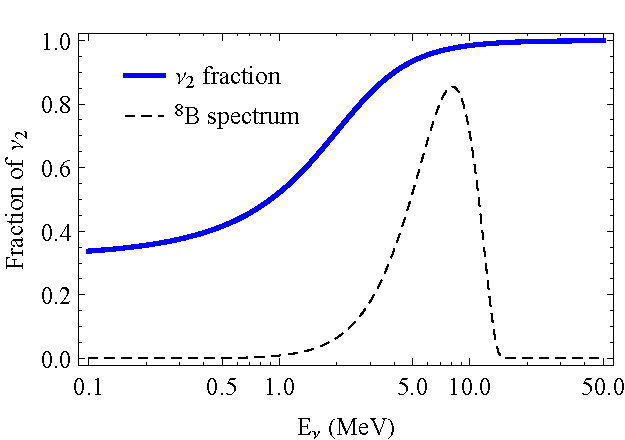
\includegraphics[width=0.75\columnwidth]{nu2_fraction}
\caption{
The fraction of $^8$B neutrinos that are $\nu_2$ upon exiting the Sun are shown here as a function of neutrino energy with a solid line, while the dashed line shows a typical $^8$B energy spectrum. 
This plot was created using central values for the neutrino mixing and standard solar model parameters. 
}
\label{fig:frac_not_nu_2}
\end{figure}

$^8$B solar neutrinos are produced in a continuous region of the Sun, which samples a large range of electron densities.
This variation in electron density must be propagated into the modeled survival probability curves.
\Cref{fig:core_density} shows the variation in the survival probability of neutrinos from the core of the Sun to a tenth of the solar radius.
$^8$B neutrinos are primarily produced at intermediate radii.

\begin{figure}
\centering
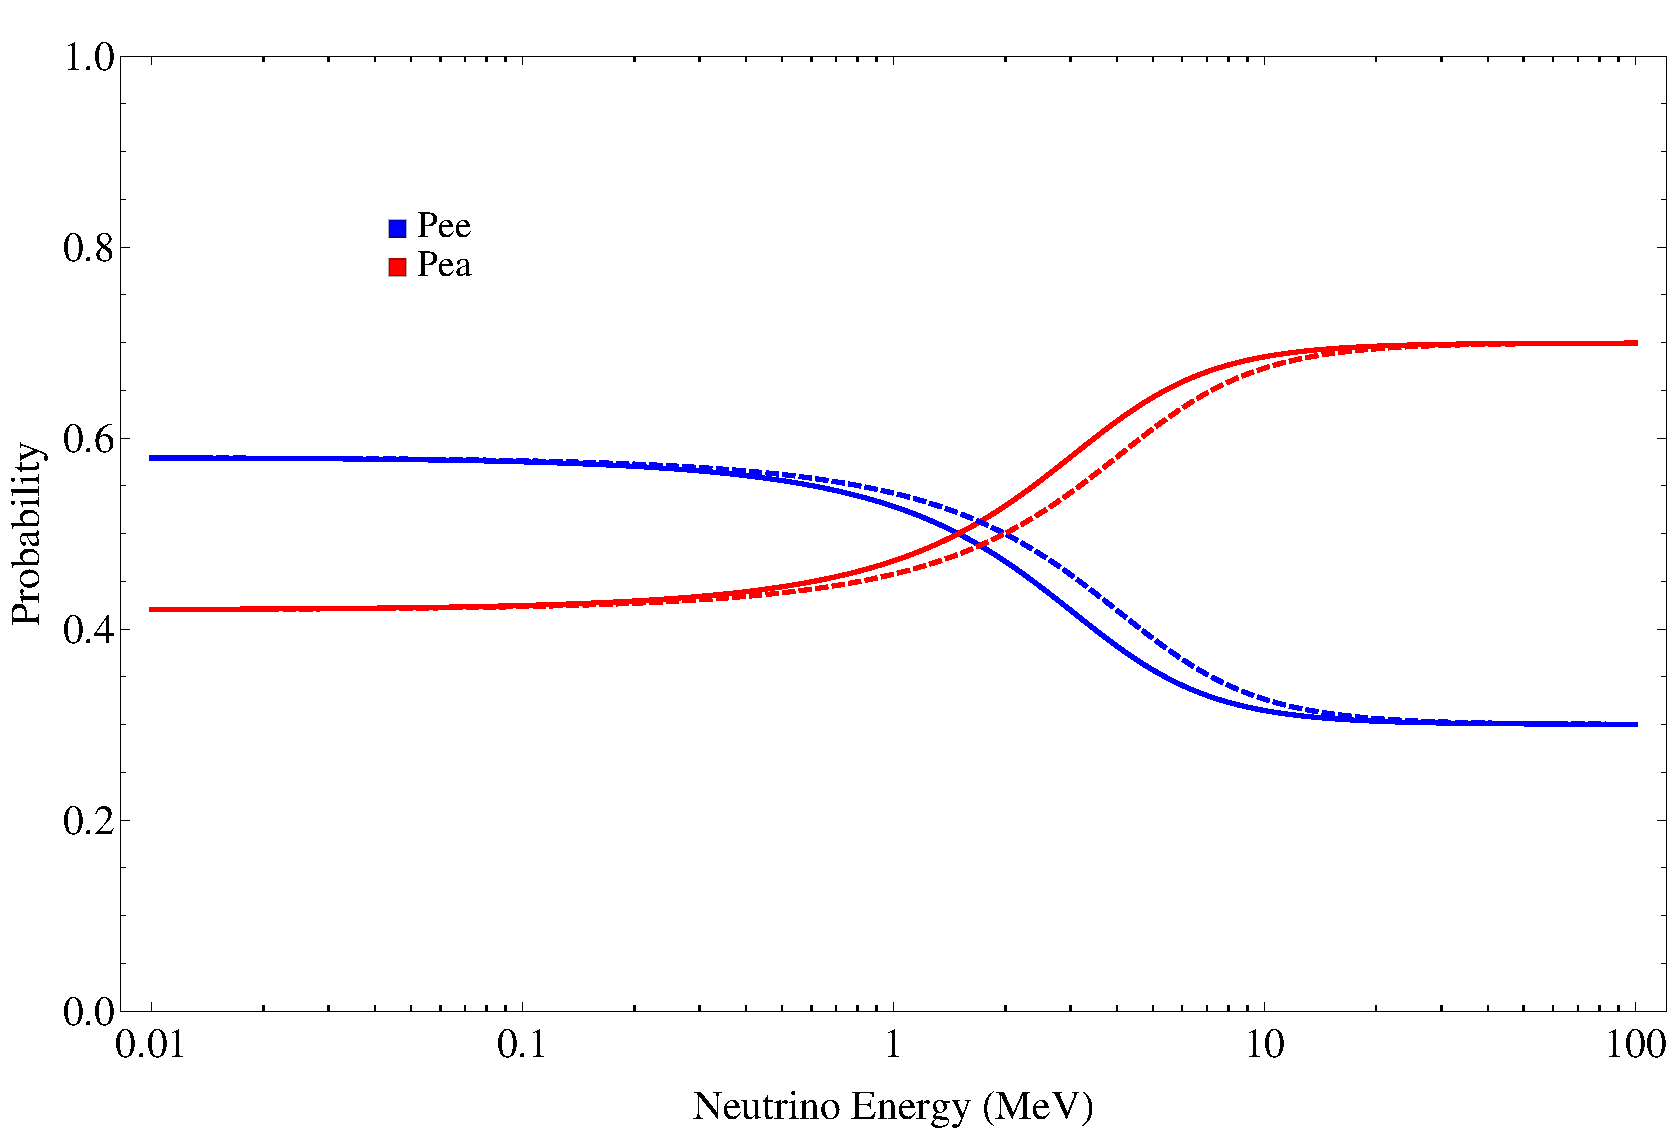
\includegraphics[width=0.75\columnwidth]{survival_core}
\caption{The solid lines here represent the MSW survival probability curves for neutrinos at the center of the solar core, with neutrinos produced a $0.1R_{\odot}$ in dashed lines. Most $^8$B neutrinos come from intermediate densities.}
\label{fig:core_density}
\end{figure}

However, because a numerical method must be used to compute the MSW effect in a three neutrino scenario, one cannot simply integrate over this variation in electron density to arrive at the average survival probability. 
To calculate the survival probability of a $^8$B neutrino numerically for a particular neutrino energy value, a MC method is used:
\begin{enumerate}
\item Generate an ensemble of radial positions sampled from the SSM radial distribution for $^8$B neutrino flux.
\item Use the SSM electron density distribution to find the electron densities for this ensemble.
\item For each electron density, numerically diagonalize the Hamiltonian $H_{MSW}$ from \Cref{eq:msw} in the flavor basis using TMatrixDEigen from ROOT~\cite{root}.
\item These eigenvectors are  $\ket{\nu_{mi}(V_e)}$, and their projection onto $\ket{\nu_e}$ is trivial in the flavor basis.
\item The quantity \Cref{decay} is calculated using these projections for a particular values of $k_i$.
\item Survival probabilities are calculated with \Cref{survive} and averaged across the ensemble.
\end{enumerate} 

This process can be executed for any neutrino energy, producing survival probability curves for neutrinos produced in regions consistent with $^8$B neutrinos.
Example survival/oscillation probability curves produced this way for different values of $k_2$ are shown in \Cref{fig:model}.

\begin{figure}
\centering
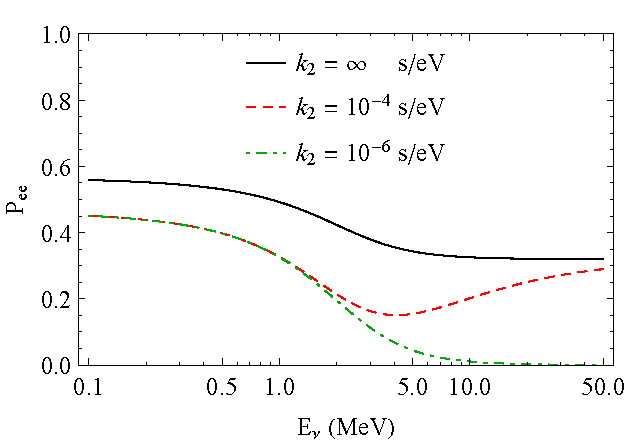
\includegraphics[width=0.75\columnwidth]{decay_msw_pee_theory}
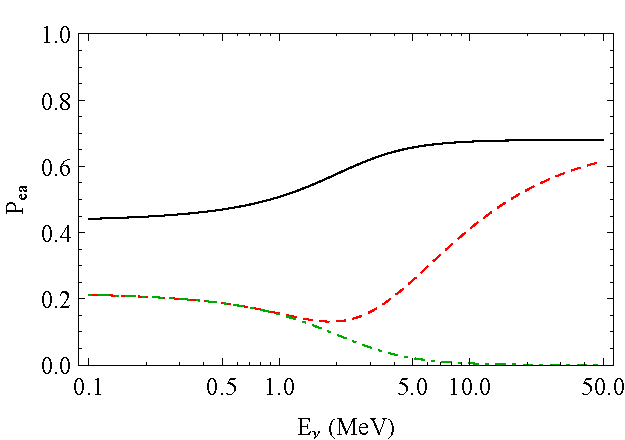
\includegraphics[width=0.75\columnwidth]{decay_msw_pea_theory}
\caption{
Shown here in dashed lines are survival probability of
electron neutrinos $P_{ee}$ and the oscillation probability $P_{ea}$ for
various values of mass state $\nu_2$ lifetime ($k_2$), demonstrating the
energy-dependent distortion being modeled. Both $k_1$ and $k_2$ are fixed
to infinity in these plots. Existing limits are near $k_2 = 10^{-4}$ s/eV.
The solid line shows the survival probability with no neutrino
decay ($k_2 = \infty$).
}
\label{fig:model}
\end{figure}

\subsection{Parameters}
\label{parameters}

The parameters of the neutrino lifetime model beyond the quantity of interest, the lifetime $k_2$ of mass state $\nu_2$, are discussed in the following sections.
In all cases, fundamental constants are taken from the Particle Data Group (PDG)~\cite{pdg}.

\subsubsection{Neutrino Mixing}
Neutrino mixing parameters taken from KamLAND~\cite{kamland} and Daya Bay~\cite{dayabay} are reproduced in \Cref{tbl:mixing_params}. 
Parameters from KamLAND and Daya Bay were used to avoid bias from using SNO results in this analysis.
As these measurements were done at Earth with neutrinos produced on Earth, they are expected to be uncorrelated with effects of $\nu_2$ decay.
The current limit on $k_2$ constrains it to be greater than $\approx7\times10^{-4}$~\cite{picoreti}, which means at length scales comparable to the diameter of the earth the maximum flux lost by $\nu_2$ decay for a $10$ MeV neutrino is given by
$1-e^{-2R_{earth}/(E k_2)} \approx 6\times10^{-6}$,
which would have negligible impact on values quoted for mixing parameters.

\begin{table}
\centering
\begin{tabular}{c|c|c}
Parameter & Value & Ref \\ \hline
$ \Delta m ^2 _{21} $ & $7.58^{+0.14}_{-0.13}(stat)^{+0.15}_{-0.15}(syst) \times 10^{-5}$~eV$^2$ &~\cite{kamland} \\ \hline
$ \tan^2 \theta_{12} $ & $0.56^{+0.10}_{-0.07}(stat)^{+0.10}_{-0.06}(syst) $ &~\cite{kamland} \\ \hline
$ |\Delta m ^2 _{32}| $ & $2.45\pm0.06(stat)\pm0.06(syst) \times 10^{-3}$~ev$^2$ &~\cite{dayabay} \\ \hline
$ \sin^2 2\theta_{13} $ & $0.0841\pm0.0072(stat)\pm0.0019(syst)$ &~\cite{dayabay} \\ \hline
$ \sin^2 \theta_{23} $ & $0.5^{+0.058}_{-0.062}$ &~\cite{superkth23} \\ 
\end{tabular}
\caption{
\label{tbl:mixing_params}
Reproduced here are the mixing parameters used in this analysis taken from Daya Bay~\cite{dayabay}, Super-Kamiokande~\cite{superkth23}, and KamLAND~\cite{kamland} results.
}
\end{table}

\subsubsection{Standard Solar Model}

The model implemented here uses the distribution of electron density and distribution of neutrino fluxes calculated in the BS05(OP) Standard Solar Model (SSM)~\cite{bs05op}, which are reproduced in \Cref{fig:ssm}. 
Uncertainties in these values are not quoted in the original source and are therefore not considered here.
These predictions are expected to be unaffected by potential $\nu_2$ decay as they are not constrained with neutrino flux measurements.

\begin{figure}
\centering
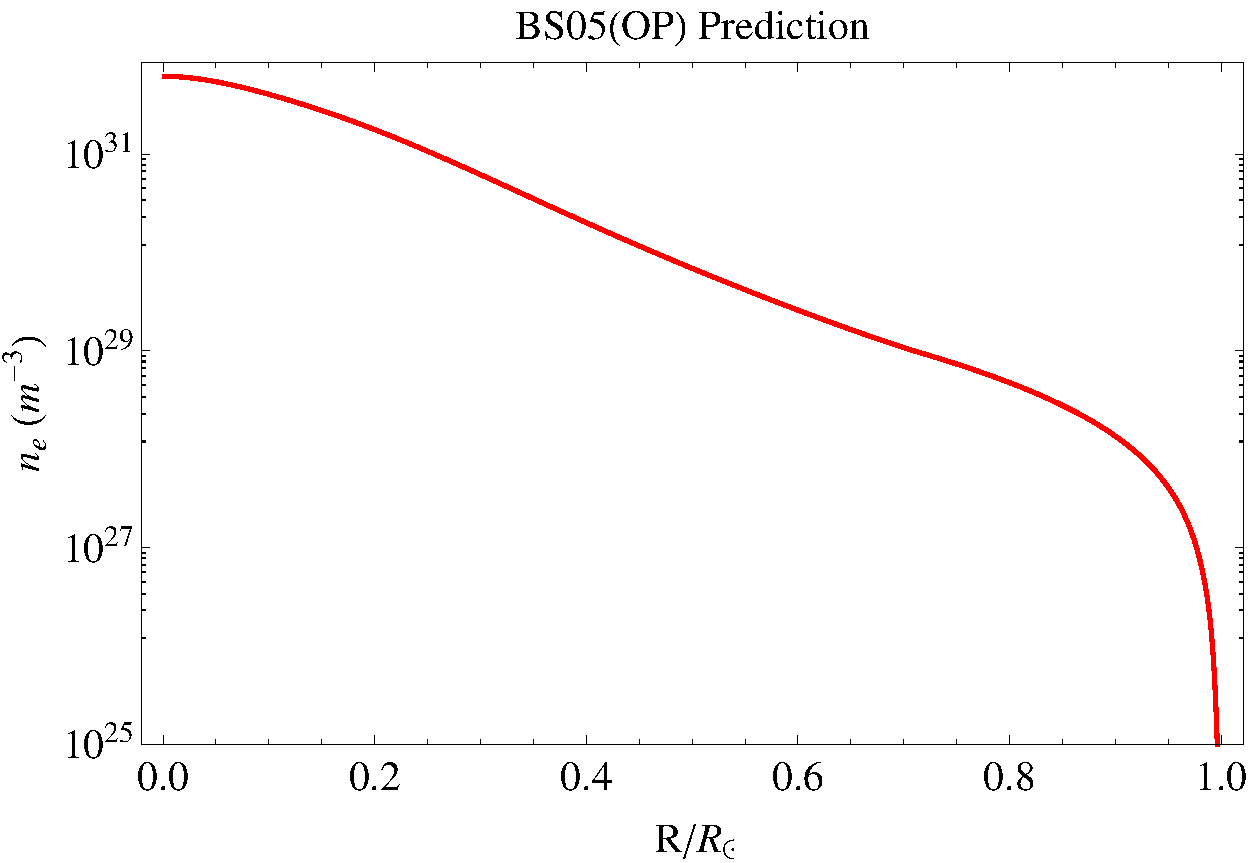
\includegraphics[width=0.48\columnwidth]{ssm_ne}
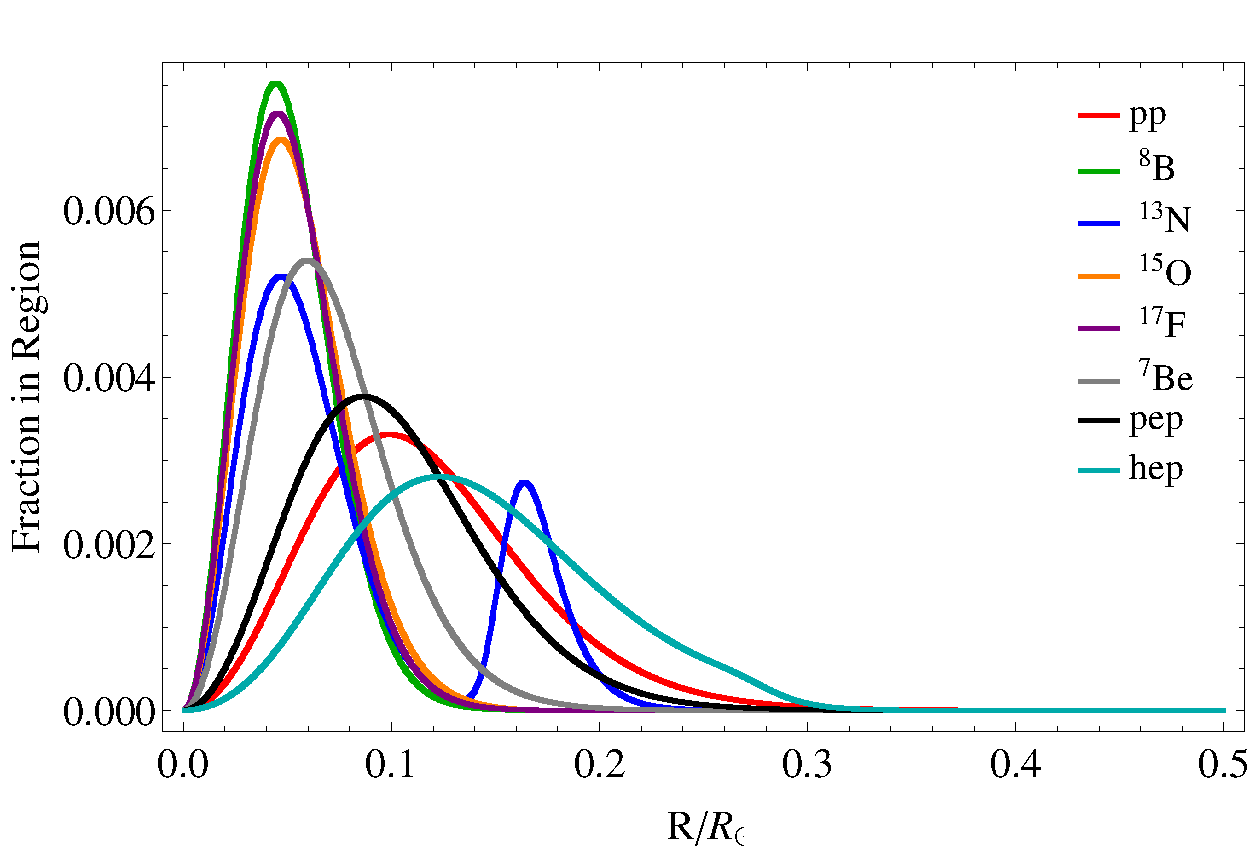
\includegraphics[width=0.48\columnwidth]{ssm_nu_region}
\caption{
The electron density in the Sun as a function of radius and the fraction of the neutrino flux produced in a radial region as a function of radius for the different neutrino fluxes. Only the $^8$B flux is relevant for this data. From the BS05(OP) SSM~\cite{bs05op}.
}
\label{fig:ssm}
\end{figure}

\subsubsection{$^8$B Flux}

As earth bound measurements of the solar neutrino flux would be biased by neutrino decay, a theoretical prediction for the $^8$B flux is required.
Serenelli's most recent prediction yields a $^8$B flux of $5.88\times10^{6}$~cm$^{-2}$s$^{-1}$ with $11\%$ uncertainty~\cite{serenelli}, which is used as a prior in this fit.
For reference the flux from BS05(OP)~\cite{bs05op} traditionally used in SNO analyses is $5.69\times10^6$~cm$^{-2}$s$^{-1}$.
See \Cref{strategy} for further discussion of how the flux is handled.

\section{Fit Implementation}
\label{fit_impl}

For this analysis, I have built off the existing QSigEx code~\cite{plthesis}, which properly handled nuisance parameters, PDF generation, data binning, and likelihood function implementation for the published 3-phase analysis of SNO data~\cite{3phase}.
This package was modified to use the model described in \Cref{lifetime_model} instead of polynomials used in previous analyses.
The following sections conceptually describe how to analyze SNO data, the implementation of such an analysis in QSigEx, and the work that was necessary to implement the neutrino lifetime model in this framework.
Since QSigEx was previously vetted for SNO fits, a demonstration that the updated code produces the same results as previous analyses is given in \Cref{qsigex_validation}.

\subsection{Extended Log Likelihood}

The physical observables determined from vertex reconstruction can be used to statistically sort events into different classes of interactions.
Here the statistical sorting is done with a maximum likelihood fit: QSigEx finds the model parameters best describing the data by varying these parameters and maximizing the Poisson likelihood of the observed data.
This is done by minimizing the well known form of the log likelihood:
\begin{equation}
    \mathcal{L} = -\nu + \sum_{i=1}^{n_{events}} \log \left[ \nu f(\vec{x_i}) \right],
\end{equation}
where $\nu$ is a Poisson mean number of observed events and $f(\vec{x_i})$ is a PDF evaluated $\vec{x_i}$, which is a vector of quantities describing event $i$.
In the case of many classes of events with Poission parameters $\nu_j$ decribed by PDFs $f_j$ this log likelihood this can be written as:
\begin{equation}
    \mathcal{L} = -\sum_{j=1}^{n_{classes}} \nu_j + \sum_{i=1}^{n_{events}} \log \left[ \sum_{j=1}^{n_{classes}} \nu_j f_j(\vec{x_i}) \right].
\end{equation}
In a typical SNO analysis, each type of signal or background for each phase is treated as a separate event class.
When the rates of these classes are expected to be correlated across phases, the Poisson parameter for those classes are constrained to be the same value.
In this way one can simultaneously fit to all three phases of SNO data in a self consistent manner.

\subsection{Analyzing SNO Data}
\label{sec:sno_observables}

In SNO the observable quantities of choice are:
\begin{enumerate}
    \item Energy - the estimated deposited energy assuming Cherenkov light from an electron. Necessary for recovering spectral information for solar neutrinos and disentangling low energy backgrounds from higher energy solar neutrinos.
    \item Radius - the volume weighted radius of the event estimated from reconstruction. Useful for distinguishing neutrino events, which are isotropic within the detector from intrinsic radioactivity, which is maximal at higher radii due to a very successful background reduction campaign within the AV.
    \item Isotropy - the $\beta_{14}$ parameter based on Legendre polynomials giving a direction independent measure of isotropy of hits. Can distinguish between multi site events (multiple gammas scattering multiple electrons - NC) and single electrons (CC, ES). Also capable of discriminating between physics events (Cherenkov hit topology) and instrumental backgrounds.
    \item Direction - the cosine of the angle between the reconstructed event direction and the direction to the Sun at the time of the event. Identifies ES electrons, which are highly correlated with the solar direction, and provides some discrimination for CC electrons.
\end{enumerate}
These observables were chosen to maximize separation between different types of physics interactions (NC, CC, ES) and of physics, backgrounds, and instrumentals. 
To properly take into account correlations between these parameters, 4D PDFs were used instead of four separate 1D PDFs.
A notable exception is the inclusion of Phase III data, where the NCDs present in the target volume significantly complicated photon propagation, and made $\beta_{14}$ a less reliable metric than in Phases I and II.
For Phase III, 3D PDFs in energy, radius, and direction were used.

The likelihood fit determines the relative contribution of each event class necessary to best match the observed data.
To do this, the fit needs the 4D PDF for each type of event, and these PDFs were generated using a MC method.
SNOMAN~\cite{sno_nim} was a FORTRAN simulation package developed by SNO that was adjusted to reproduce calibration data taken with the detector.
The reconstruction algorithms used on raw data were applied to the simulation results of SNOMAN for known classes of interactions to produce the PDFs used in analysis.

Most PDFs are constructed by directly binning simulated data produced by SNOMAN.
The physics encoded by the neutrino survival probabilities is included by reweighting solar neutrino events from SNOMAN while building the PDFs for solar signals.
For the radioactivity of the PMT glass, only tails of this high-rate background fall within the ROI, and it was impractical to simulate a sufficient number of interactions to produce reliable PDFs.
In this case, analytical forms were used instead, and the parameters controlling these analytical forms were estimated from the data and treated as systematic uncertainties.

\subsection{Building Solar PDFs}

There are two options for handling the neutrino energy dependence in such a fit:
\begin{itemize}
\item Binned neutrino energy fits where where the neutrino MC is binned into $N$ PDFs by neutrino energy prior to the fit, and the average value of the survival probability across that entire bin is applied to each of the $N$ PDFs when stepping though the minimization.
\item Unbinned neutrino energy fits where each of the $M >> N$ neutrino MC events are reweighted by the value of the survival probability at their exact energy when stepping through the minimization to build the neutrino PDFs.
\end{itemize}
Clearly the binned fit will perform more poorly as an average value of the survival probability across a neutrino energy bin is applied to all neutrinos in that bin, however, this method is much faster, being computationally far simpler than rebuilding the PDFs at each minimization step. 
For polynomial fits of previous SNO analyses, this poorer performance was not significant and allowed the minimization algorithm to benefit from the increased speed.
Unfortunately preliminary tests of the binned fit had very poor results regarding capturing the shape of the lifetime model survival probabilities.
Because of this, an unbinned neutrino energy fit was adopted.

\subsection{Detector Systematic Effects}
\label{systematics} 

Systematic uncertainties are treated in three distinct ways.
\begin{enumerate}
\item Each of the observables has many systematic parameters associated with it representing possible discrepancies between simulated and real data. These uncertainties are best constrained with the data itself, and most likely central values along with their uncertainties are determined with an initial brute-force iterative scan of each parameter while maximizing the likelihood of the data. These parameters are then held fixed during the central fit, and uncertainties are propagated with a shift-and-refit method.
\item Other uncertainties are best constrained with in-situ and ex-situ measurements and not highly correlated with neutrino parameters. These are also held fixed during the central fit, and uncertainties are propagated with a shift-and-refit method.
\item Finally, the NCD neutron capture efficiency, which is strongly correlated with measurements of the neutrino flux, is allowed to float in the fit to avoid biasing neutrino results.
\end{enumerate}

The procedure for determining the central values and uncertainties of scanned parameters is as follows:
\begin{enumerate}
\item A parameter is scanned around its current best guess with other systematics held at their best guess.
\item At each point in the scan, the minimization algorithm is run, finding the minimum negative log likelihood value.
\item This produces a negative log likelihood profile as a function of the parameter of interest.
\item An asymmetric Gaussian is fit to the profile of the negative log likelihood to determine the central and upper/lower uncertainties for the parameter.
\item The best guess for that parameter is updated to the central value of that fit.
\item The next parameter is considered at step 1 until all parameters have been scanned.
\item If any parameter central value has shifted relative to the previous iteration, the algorithm repeats until stable minima are found.
\end{enumerate}

The shift-and-refit algorithm is intended to stochastically marginalize over the bulk of the systematic uncertainties. 
This was done for two reasons.
First, variation in many of the systematics result in events moving between bins and discontinuities in the likelihood space, which interfere with minimization algorithms.
Stochastic methods are not susceptible to such discontinuities.
Second, there are very many systematic uncertainties, and floating them all would result in an intractably large parameter space.
Therefore those systematic uncertainties not strongly correlated with neutrino parameters are treated with the following shift-and-refit procedure to propagate their uncertainties into the final results:
\begin{enumerate}
    \item A million sets of randomly sampled systematic parameters are produced by sampling asymmetric Gaussian distributions of parameter uncertainties. These distributions are either known from independent analyses or determined by initial scans of the dataset. 
    \item For each set of parameters, the fit is minimized again and the central value of each floated parameter is recorded.
    \item This produces a distribution of shift-and-refit values for each floated parameter, which represent the systematic uncertainties on these parameters.
\end{enumerate}

If the shift-and-refit distributions are approximately normal, the upper and lower RMS represents the upper and lower systematic uncertainty. 
This applies to most floated parameters, but notably not to $k_2$, which was shown to have highly asymmetric errors. 
In the case of $k_2$, an assumption is made that the shape of the likelihood space does not change with variations in the central value of $k_2$ but rather the minimum simply shifts.
Taking this assumption, the likelihood profile for $k_2$ obtained with systematics fixed to their central values can be shifted by each shift in the shift-and-refit distribution for $k_2$ and averaged to obtain a likelihood profile including systematic uncertainties.

\subsection{Fit Strategy}
\label{strategy}
Ideally all neutrino parameters would be floated with priors in this analysis. 
In practice it has been observed that the fit does not converge with both the $^8$B flux and lifetime parameter floated unless there is a very strong external constraint on the flux.
This is most easily understood by considering the signature of neutrino decay: a disappearance of neutrino flux.
Manifestly neutrino decay and the total flux will be highly correlated, however, the energy dependent signature of neutrino decay allows these effects to be disentangled to some extent.
Previous SNO analyses searching for oscillation to sterile neutrinos~\cite{plthesis} have encountered a similar issues and opted for a strategy of finding a preferred $^8$B flux in some reduced parameter space, performing further fits and statistical studies with the flux fixed, and finally incorporating uncertainty from flux variations as a final step.
In this analysis since there is only one model parameter of interest, $k_2$, a strategy of scanning $k_2$ manually while floating all other parameters seems to be ideal. 
With that in mind, the fit strategy is:
\begin{enumerate}
\item Perform a scan over $k_2$ minimizing floated parameters at each point producing a likelihood profile. For data fits this can be done along with the other scanned nuisance parameters.
\item At the best, use MINOS fit errors (implicitly with $k_2$ fixed) as the total uncertainty on all parameters except the highly correlated $k_2$ and $^8$B flux.
\item For $k_2$ find the total uncertainty by at the point where change in negative log likelihood profile with respect to the minimum is $0.5$.
\item For the total uncertainty on $^8$B flux this value is scanned the same way as $k_2$ to properly account for the correlations in with $k_2$.
\item Combine with these uncertainties on $k_2$ and the $^8$B flux additional shift and refit uncertainties from scanned nuisance parameters.
\end{enumerate}

\section{Ensemble Testing}
\label{ensemble_tests}

To demonstrate that the fit described above is unbiased and correctly estimates errors on the fitted parameters, statistical tests were done on an ensemble of fake datasets.
These fake datasets are generated with known parameters, and the results of the fit are compared to these known quantities to demonstrate there is no systematic bias in parameter estimation.
This is done by ensuring a distribution of biases has a mean consistent with zero.
Further, statistical fluctuations resulting in biases in individual fits are compared to the errors estimated by the minimization algorithm by computing pull distributions for each parameter. 
A pull distribution with a width of 1 indicates the fit is properly estimating errors.
Finally the relative uncertainty of each parameter shows the sensitivity to each of the floated parameters.
These figures of merit are defined as:
\begin{equation}
Pull = \frac{Fit\,\,\,value - Actual\,\,\,value}{Fit\,\,\,uncertainty}
\end{equation}
\begin{equation}
Bias = \frac{Fit\,\,\,value - Actual\,\,\,value}{Actual\,\,\,value}
\end{equation}
\begin{equation}
Relative\,\,\,uncertainty = \frac{Fit\,\,\,uncertainty}{Actual\,\,\,value} \times 100\%
\end{equation}

This testing is done in three stages, starting with only solar neutrino events, and then with progressively more backgrounds added in order of importance.
For each stage of testing a plot showing the mean and width (as error bars) of the bias and pull distributions are produced.
Plots of the pull show the expected fluctuations of the mean ($1/\sqrt{n_{samples}}$) in dashed lines with the expected mean ($1 - 1/(4(n_{samples}-1))$) and fluctuation of the standard deviation ($1/\sqrt{n_{samples}}$) represented by shaded boxes.

\subsection{Fake Dataset Ensembles}

The SNO MC consists of different event classes for each phase of SNO.
Events from each class and phase are partitioned into $N$ sets with $M$ samples each. 
The remaining unused MC data for each phase and class is used for PDFs in the fit, so $N$ must be chosen to leave sufficient uncorrelated data for PDF generation.
$M$ is chosen from a Poisson distribution with a mean equal to the expected number of events for that event class and phase from previous SNO analyses~\cite{leta,ncd,3phase}.
For solar neutrino signals the BS05(OP)~\cite{bs05op} flux predictions were used in generating these fake datasets.
These sets can then be combined into fake datasets with realistic statistics containing only the event classes and phases desired.

The solar neutrino signals from SNO MC, which were generated with a flat survival probability spectrum, were reweighted with the lifetime model as described in \Cref{lifetime_model} 
A representative value of $k_2 = 10^{-4}$~s/eV was seeded into the fake sets to test the fit performance near the current limit of $\approx7\times10^{-4}$~\cite{picoreti}.

\subsection{Solar-Signal Only}
\label{3phase_sigonly}

\begin{table}
\centering
\begin{tabular}{ccc}
\hline
Phase I Event Classes & Phase II Event Classes & Phase III Event Classes  \\ \hline \hline
$^8$B CC & $^8$B CC & $^8$B CC \\
$^8$B ES (e) & $^8$B ES (e) & $^8$B ES (e) \\
$^8$B ES ($\mu\tau$) & $^8$B ES ($\mu\tau$) & $^8$B ES ($\mu\tau$) \\
$^8$B NC & $^8$B NC & $^8$B NC \\ \hline
\end{tabular}
\caption{
The solar-signal event classes included for each phase.
}
\label{tbl:sigonly_evcls}
\end{table}

It was possible to create 250 uncorrelated datasets of solar-signal only data.
The solar-signal event classes for each phase are shown in \Cref{tbl:sigonly_evcls}.
With QSigEx configured to only fit these event classes, the lifetime fit was performed on each dataset as described in \Cref{strategy}. 
The figures of merit for these tests are shown in \Cref{fig:sigonly_biaspull,fig:sigonly_reluncert}. 
In short, the results are consistent with an unbiased fit that properly estimates the fit uncertainties.

\begin{figure}
\centering
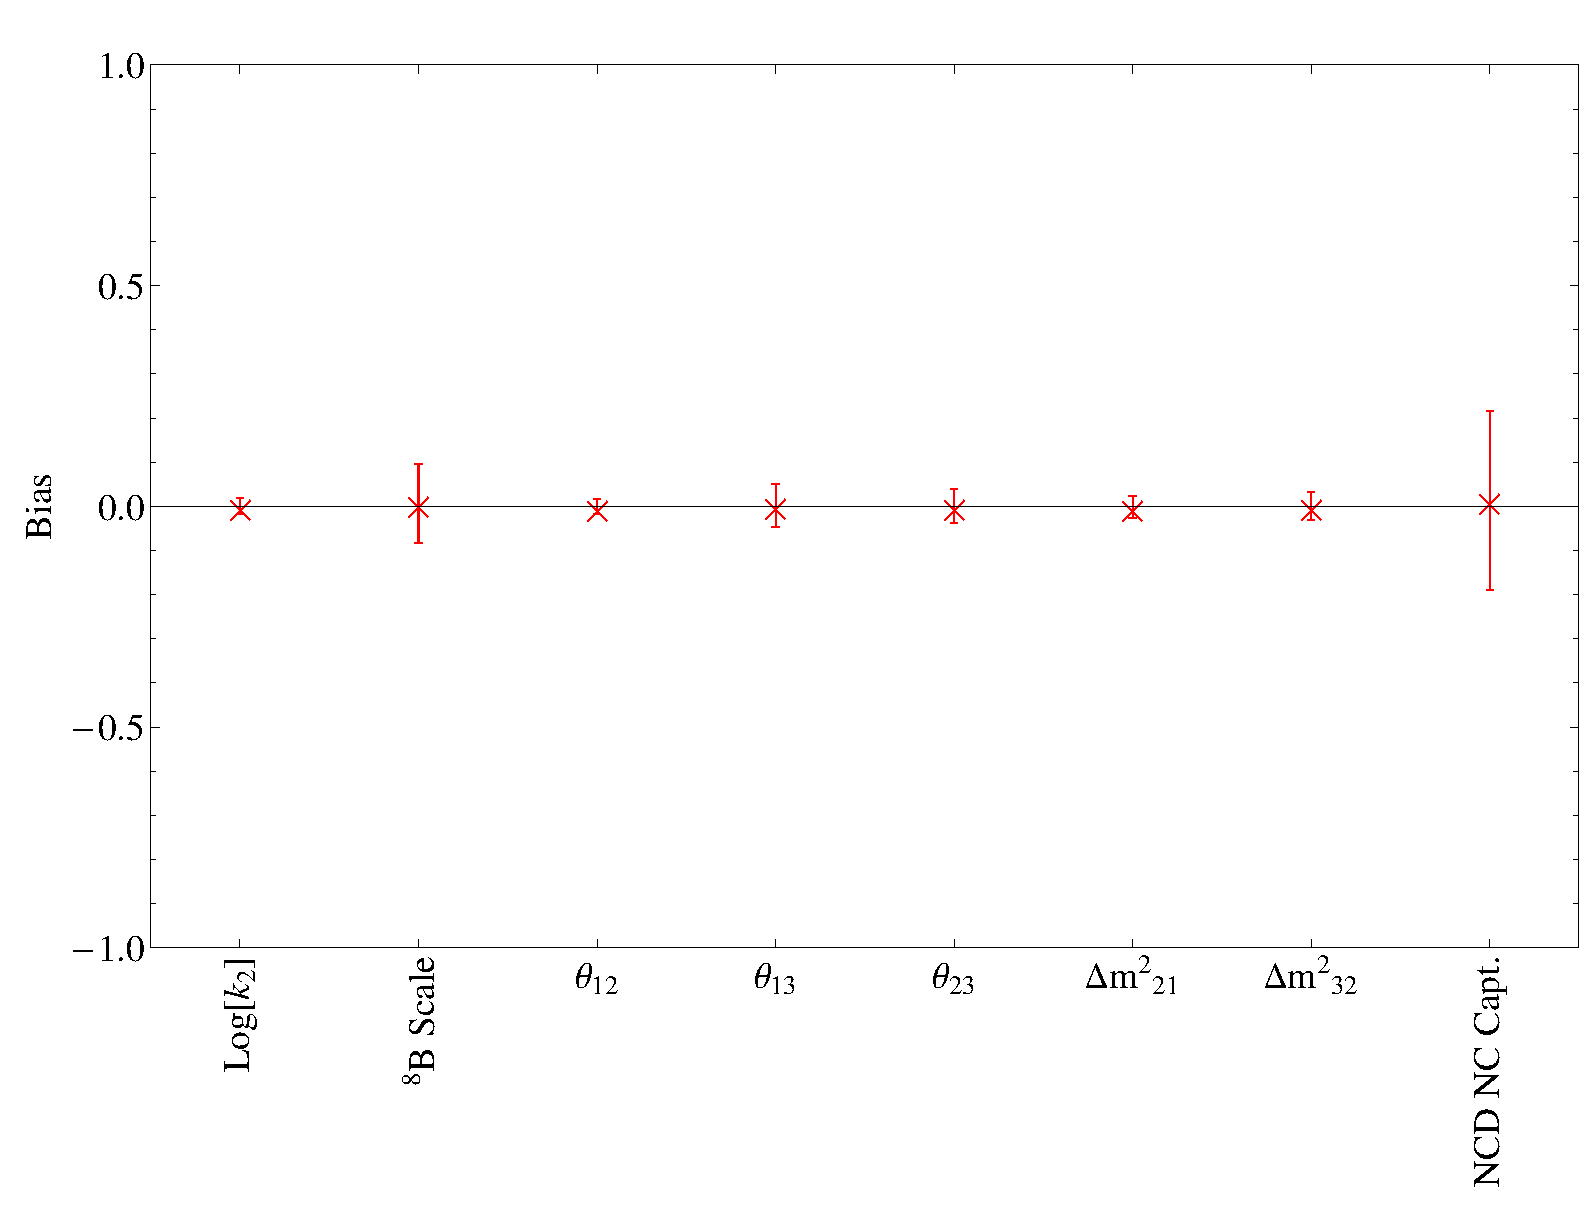
\includegraphics[width=0.80\columnwidth]{bias_nofit}
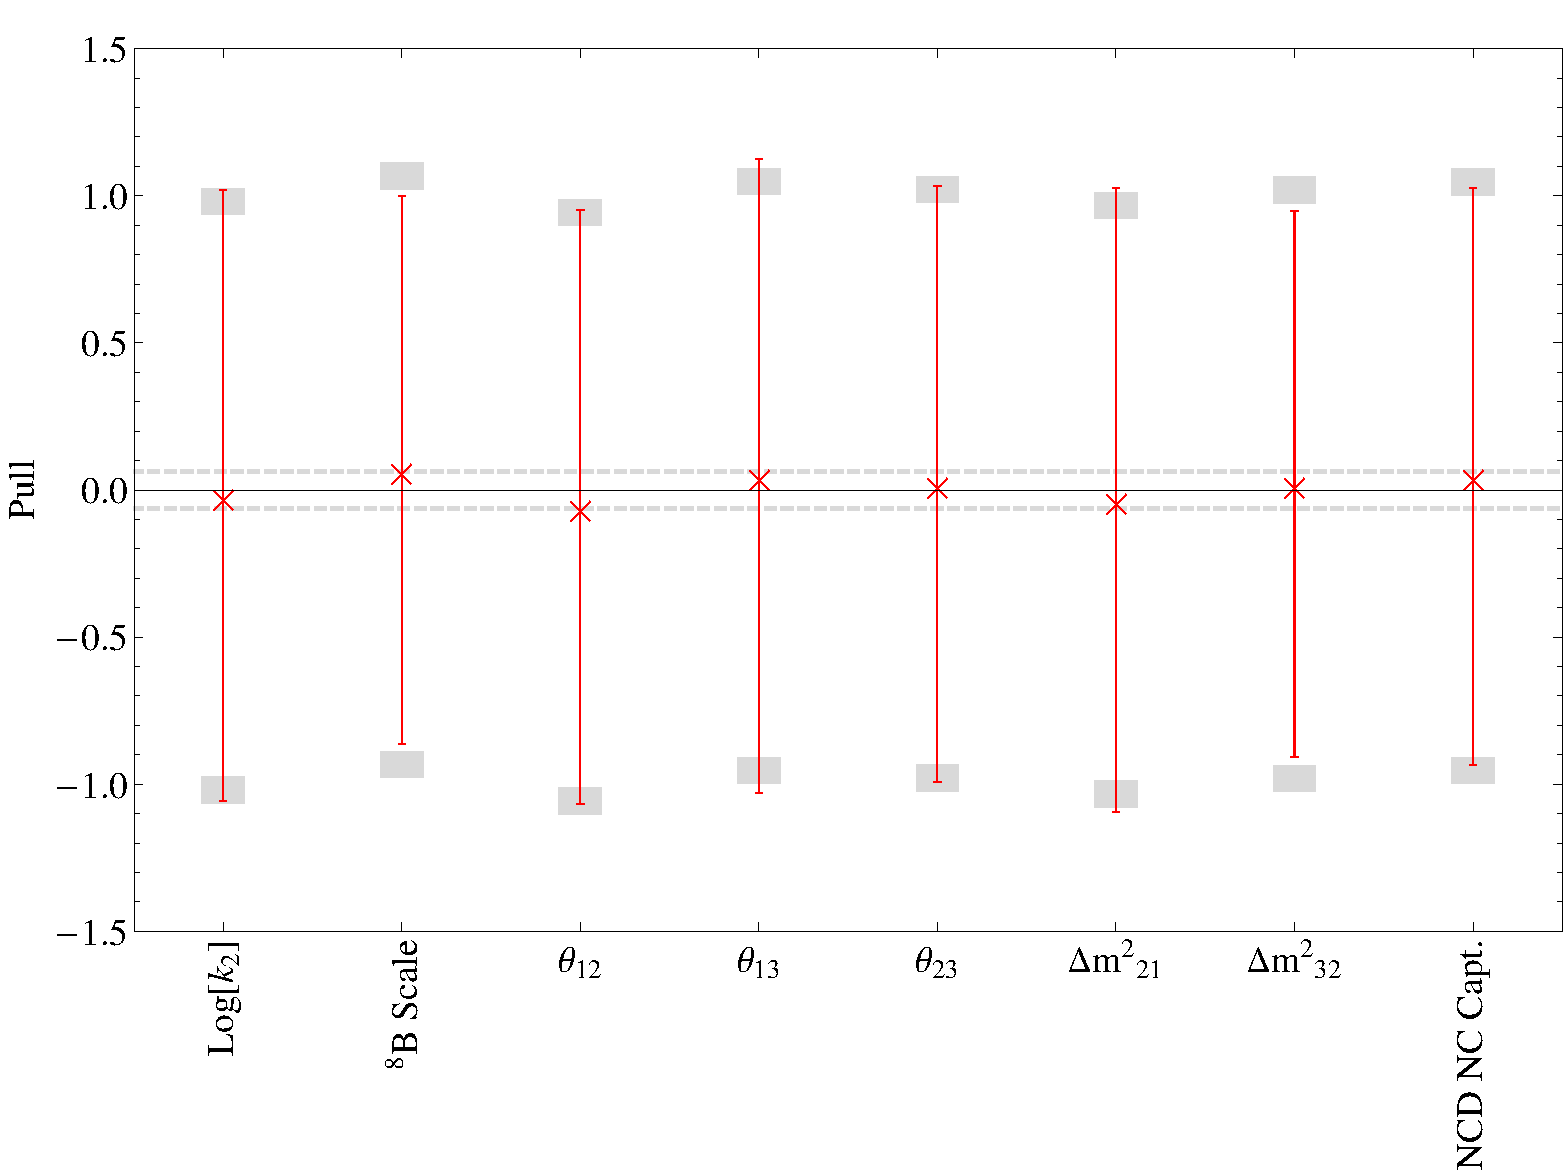
\includegraphics[width=0.80\columnwidth]{pull_nofit}
\caption{
The bias and pull of all fitted parameters with signal only datasets. Gray bars and dashed lines represent expected fluctuations due to limited statistics.
}
\label{fig:sigonly_biaspull}
\end{figure}

\begin{figure}
\centering
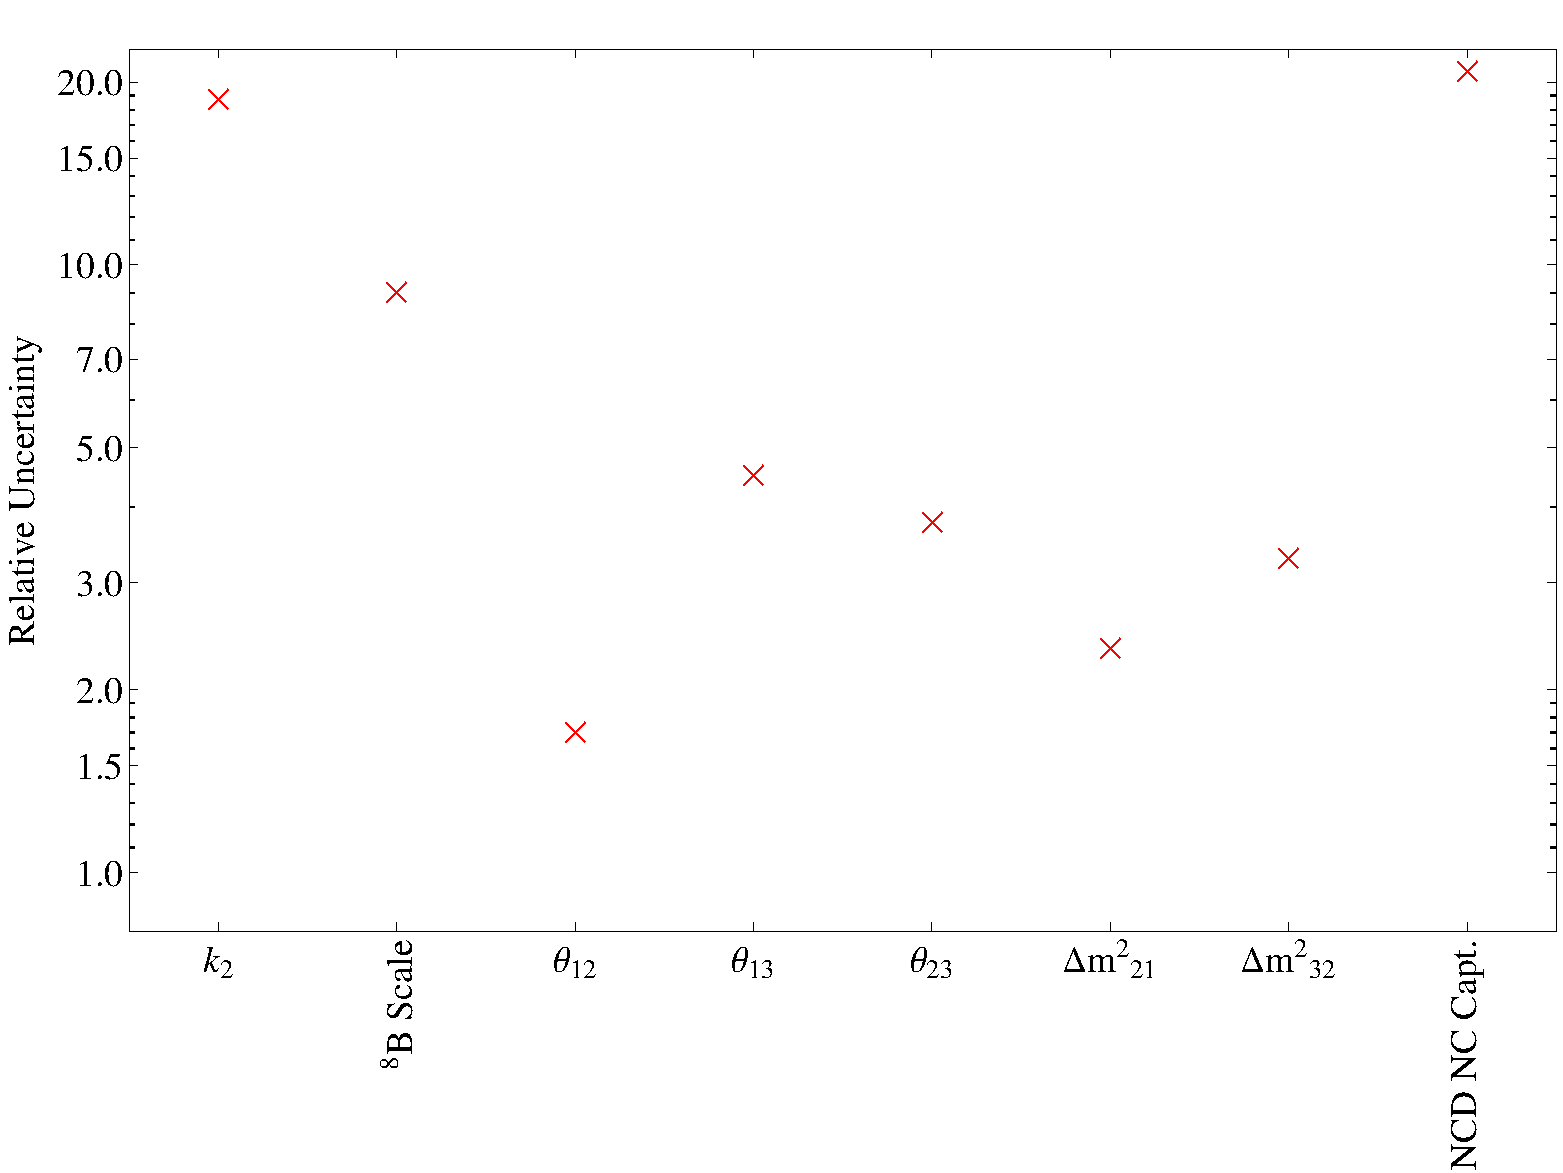
\includegraphics[width=0.85\columnwidth]{reluncert_nofit}
\caption{
The relative uncertainty of all fitted parameters with signal only datasets.
}
\label{fig:sigonly_reluncert}
\end{figure}

\clearpage

\subsection{Solar-Signal + High Statistics Backgrounds}

\begin{table}
\centering
\begin{tabular}{ccc}
\hline
Phase I Backgrounds & Phase II Backgrounds & Phase III Backgrounds \\ \hline \hline
AV neutrons & AV neutrons & External neutrons \\
Bi D$_2$O & Bi Salt & D$_2$O p.d. \\ 
Tl D$_2$O & Tl Salt & Atmospherics \\
hep CC & hep CC & hep CC \\
hep ES & hep ES & hep ES \\
hep NC & hep NC & hep NC \\
PMT $\beta$-$\gamma$ & PMT $\beta$-$\gamma$ \\ \hline
\end{tabular}
\caption{
These are the background event classes that are included in the high statistics background tests. This includes internal backgrounds, AV neutrons, PMT backgrounds, and other backgrounds with very high MC statistics.
}
\label{tbl:noextbitl_event_classes}
\end{table}

A subset of the fake 3-phase solar-signal only datasets from above were taken and combined with uncorrelated datasets of background events with high statistics.
The event classes shown in \Cref{tbl:noextbitl_event_classes} were added in this section. 
Due to the relatively lower statistics for background event classes, only 50 datasets could be created for each of the three $k_2$ values.
With QSigEx configured to only fit these event classes, the lifetime fit was performed on each dataset as described in \Cref{strategy}. 
The figures of merit for these tests are shown in \Cref{fig:noextbitl_bias,fig:noextbitl_pull,fig:noextbitl_reluncert}. 
Again, the results are consistent with an unbiased fit that properly estimates the fit uncertainties.

\begin{figure}
\centering
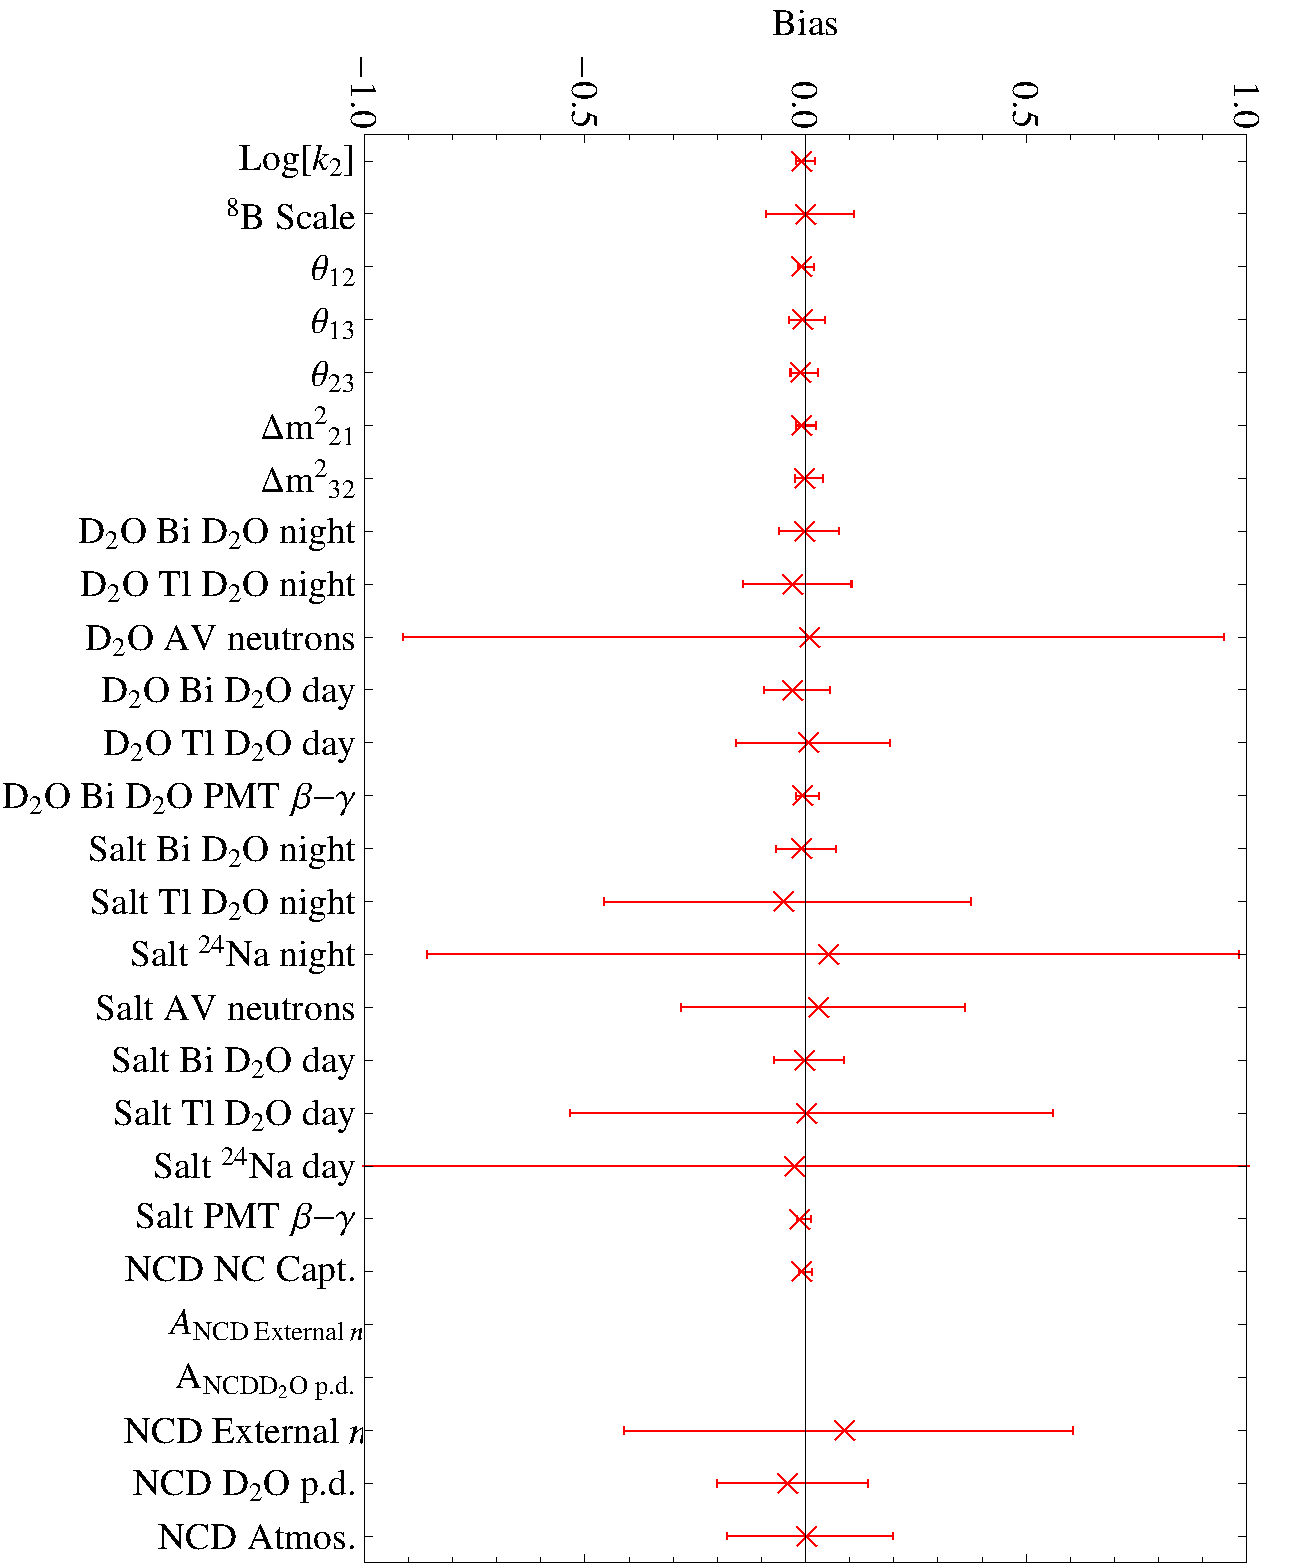
\includegraphics[height=0.85\columnwidth,angle=90]{noextbitl_bias_nofit}
\caption{
The bias of all fitted parameters with signal + high stats backgrounds datasets.
}
\label{fig:noextbitl_bias}
\end{figure}

\begin{figure}
\centering
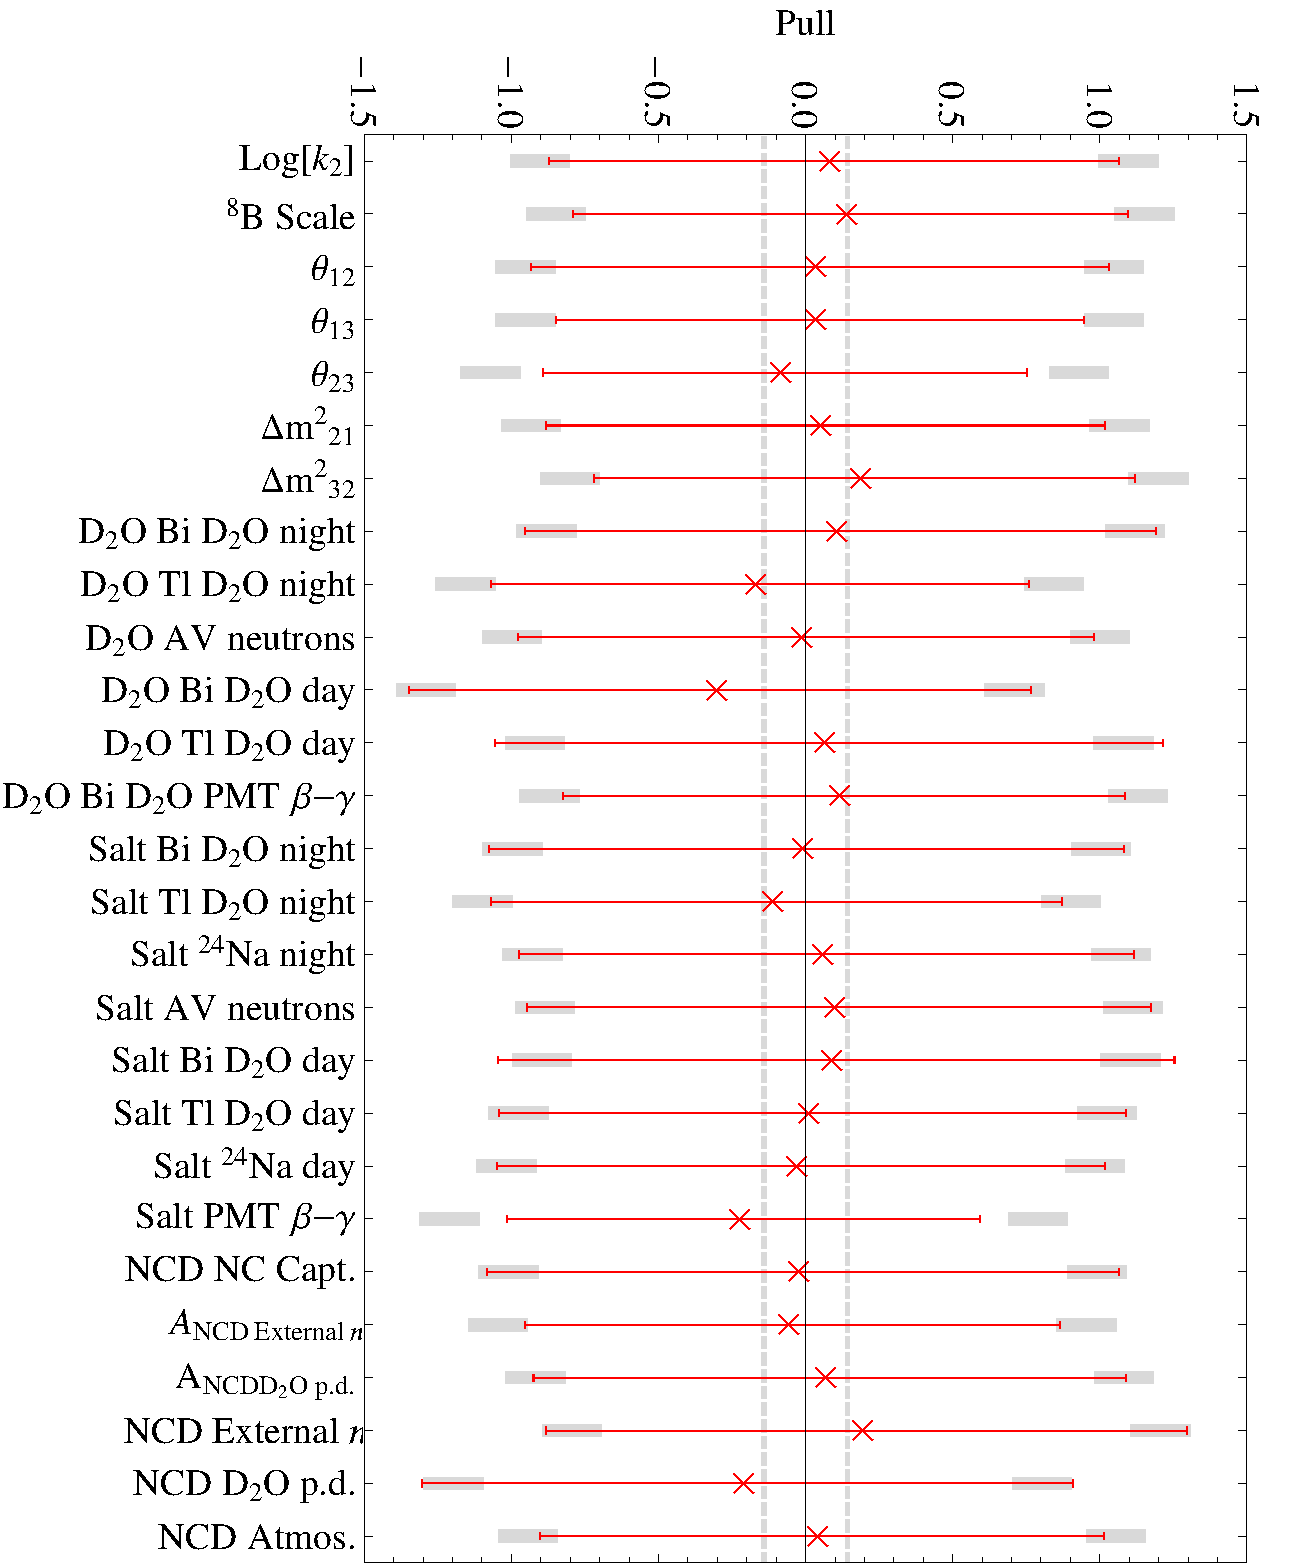
\includegraphics[height=0.85\columnwidth,angle=90]{noextbitl_pull_nofit}
\caption{
The pull of all fitted parameters with signal + high stats backgrounds datasets. Gray bars and dashed lines represent expected fluctuations due to limited statistics.
}
\label{fig:noextbitl_pull}
\end{figure}

\begin{figure}
\centering
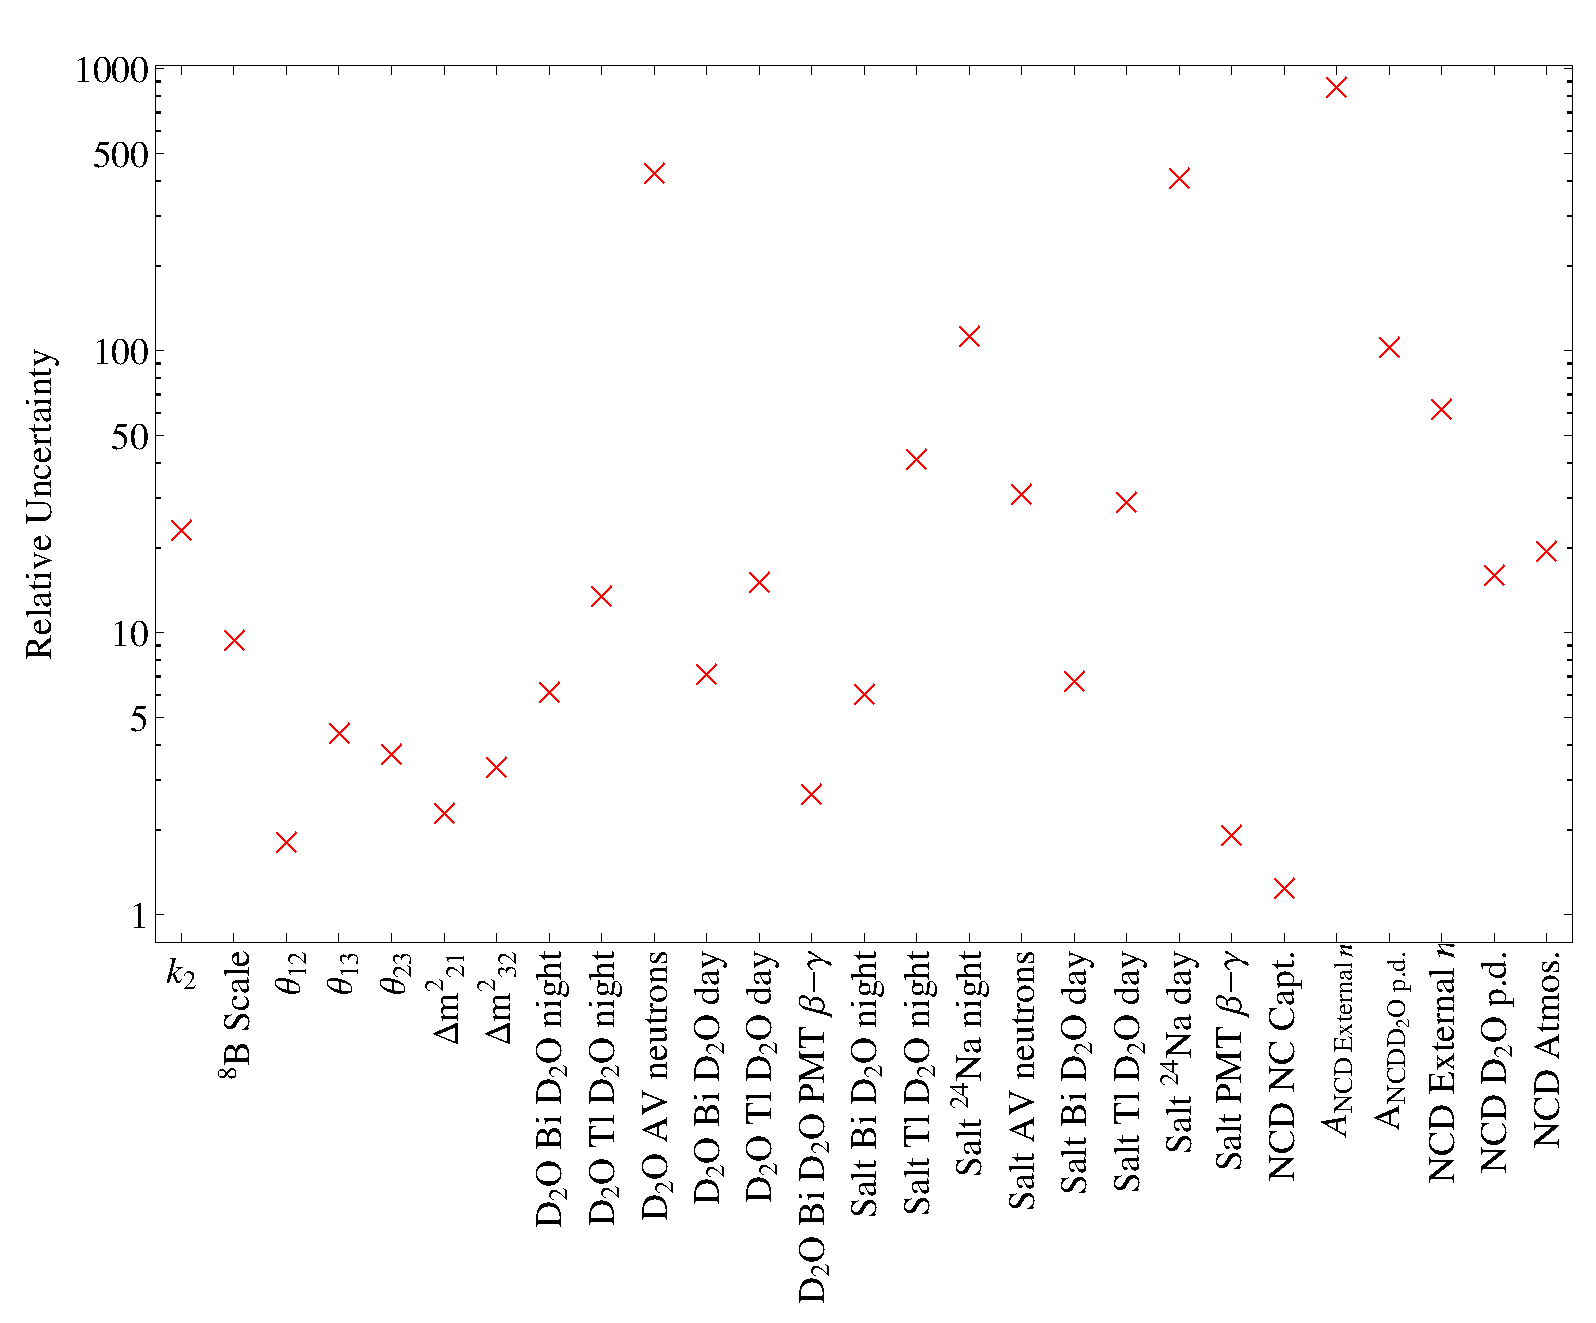
\includegraphics[height=0.85\columnwidth,angle=90]{noextbitl_reluncert_nofit}
\caption{
The relative uncertainty of all fitted parameters with signal + high stats backgrounds datasets.
}
\label{fig:noextbitl_reluncert}
\end{figure}

\clearpage

\subsection{Solar-Signal + All Backgrounds}
\label{3phase_allbg}

\begin{table}
\centering
\begin{tabular}{ccc}
\hline
Phase I Backgrounds & Phase II Backgrounds & Phase III Backgrounds\\ \hline \hline
Bi AV bulk & Bi AV bulk & Strings p.d. \\
Tl AV bulk & Tl AV bulk & K2 p.d. \\
Bi H$_2$O & Bi H$_2$O & K5 p.d. \\
Tl H$_2$O & Tl H$_2$O & \\ \hline
\end{tabular}
\caption{
These are the background event classes that are added for the fits that include all backgrounds. This includes AV and external backgrounds for Phases I and II and photodisintegration for Phase III.
}
\label{tbl:allbg_event_classes}
\end{table}

A subset of the fake 3-phase high statistics background datasets from above were taken and combined with uncorrelated datasets of background events classes with low statistics.
The event classes shown in \Cref{tbl:allbg_event_classes} were added in this section and the datasets now include all relevant event classes.
Due to extremely limited statistics for some of these event classes, only 14 datasets for each of the three $k_2$ values could be created.
As was traditionally done for SNO analyses~\cite{plthesis}, these same events were resampled with a different random seed into 14 alternate datasets (c.f. the bootstrap method).
Comparing the results of these two datasets gives some information on statistical fluctuations due to limited statistics.
If the bias or pull looks particularly bad in one dataset but acceptable in the other, one can conclude that this effect is due to statistical fluctuations and not to errors in the fit procedure.
The figures of merit for these tests are shown in \Cref{fig:allbg_bias,fig:allbg_pull,fig:allbg_reluncert}. 
While fluctuations are larger, comparison between the two datasets looks more reasonable. 
Notably these results are comparable to ensemble testing of the published SNO 3-phase results~\cite{3phase}.
One can therefore conclude that the fit is unbiased and properly predicting errors.

\begin{figure}
\centering
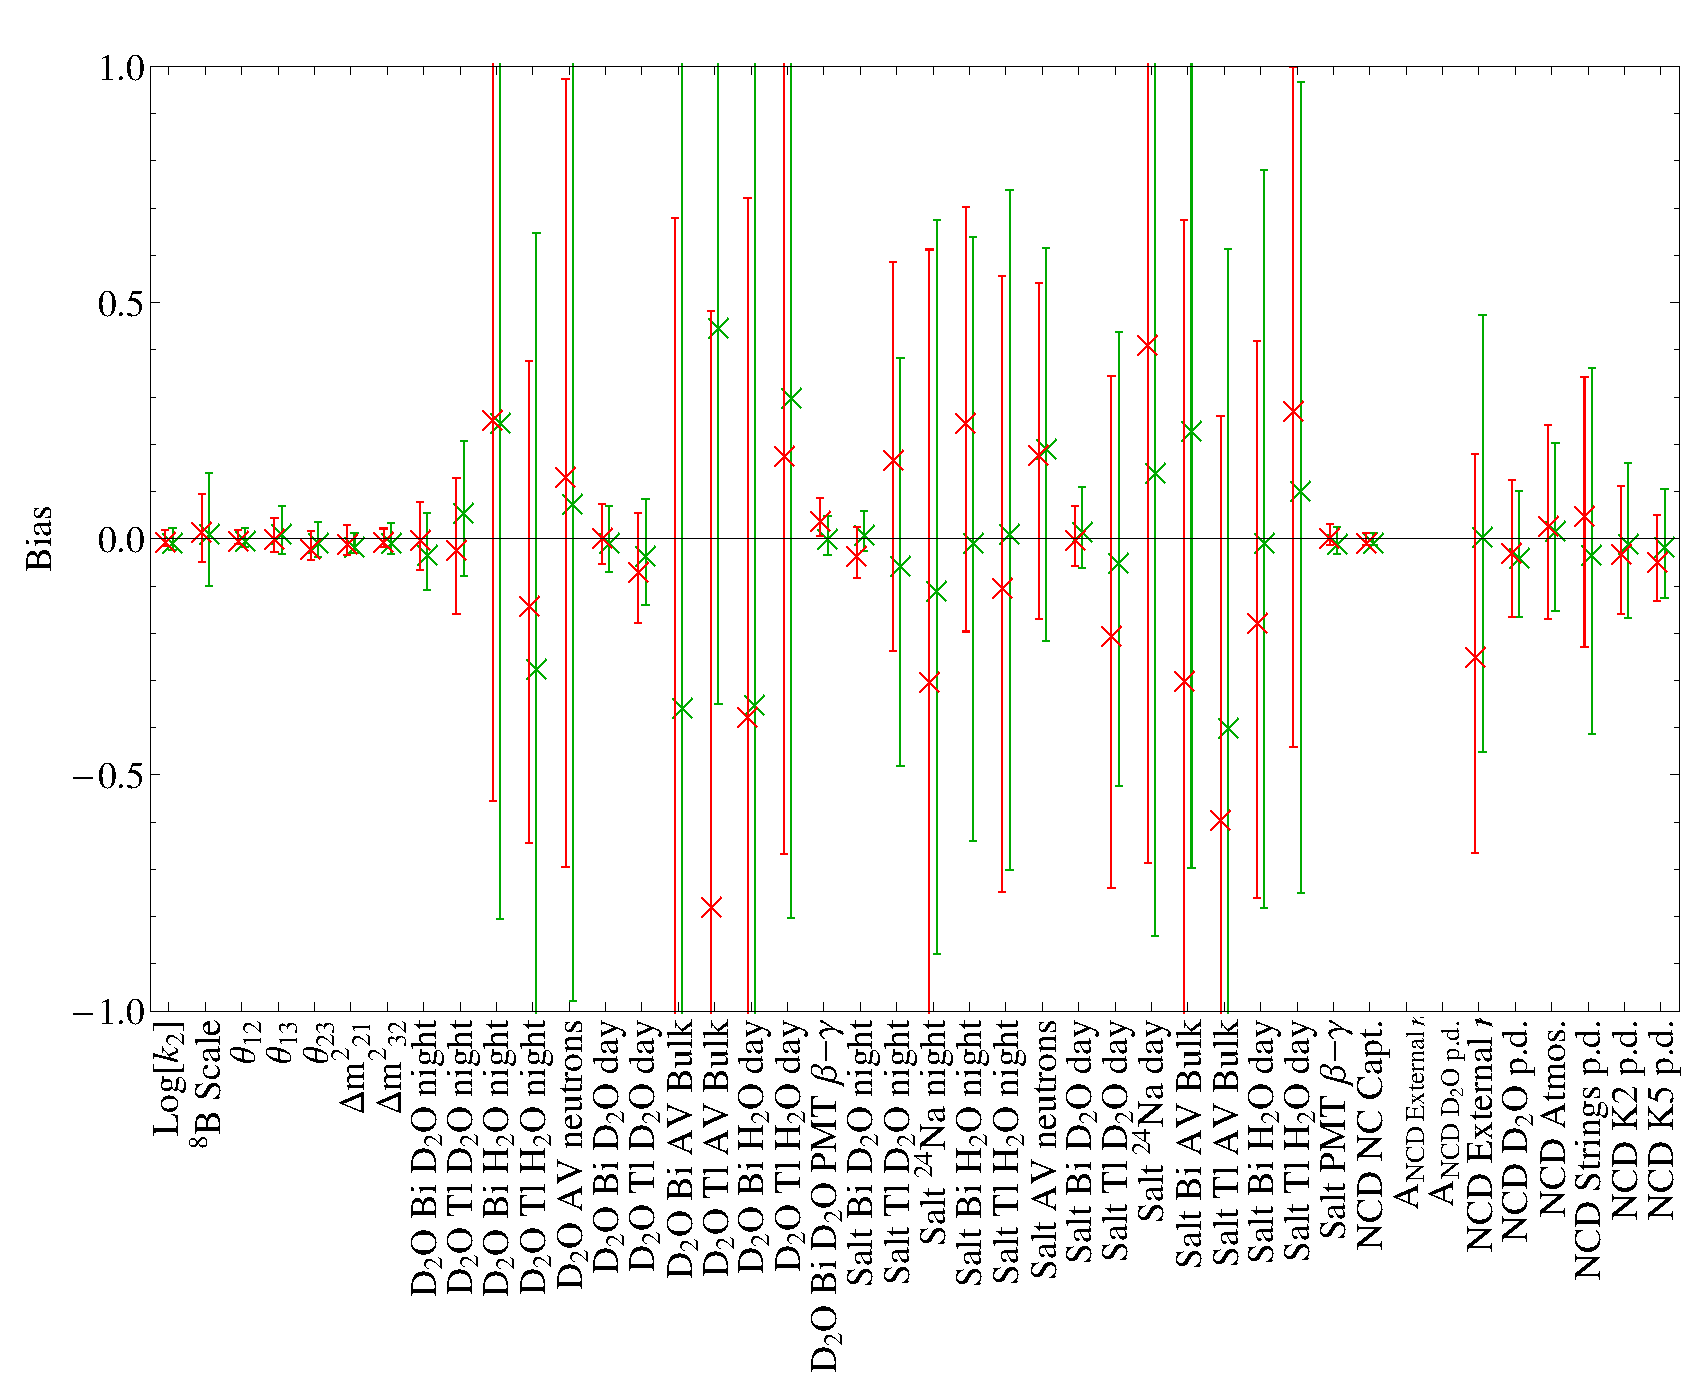
\includegraphics[height=0.85\columnwidth,angle=90]{bias_combined}
\caption{
The bias of all fitted parameters with signal + all backgrounds datasets. The alternate ensemble results are shown in green for comparison.
}
\label{fig:allbg_bias}
\end{figure}

\begin{figure}
\centering
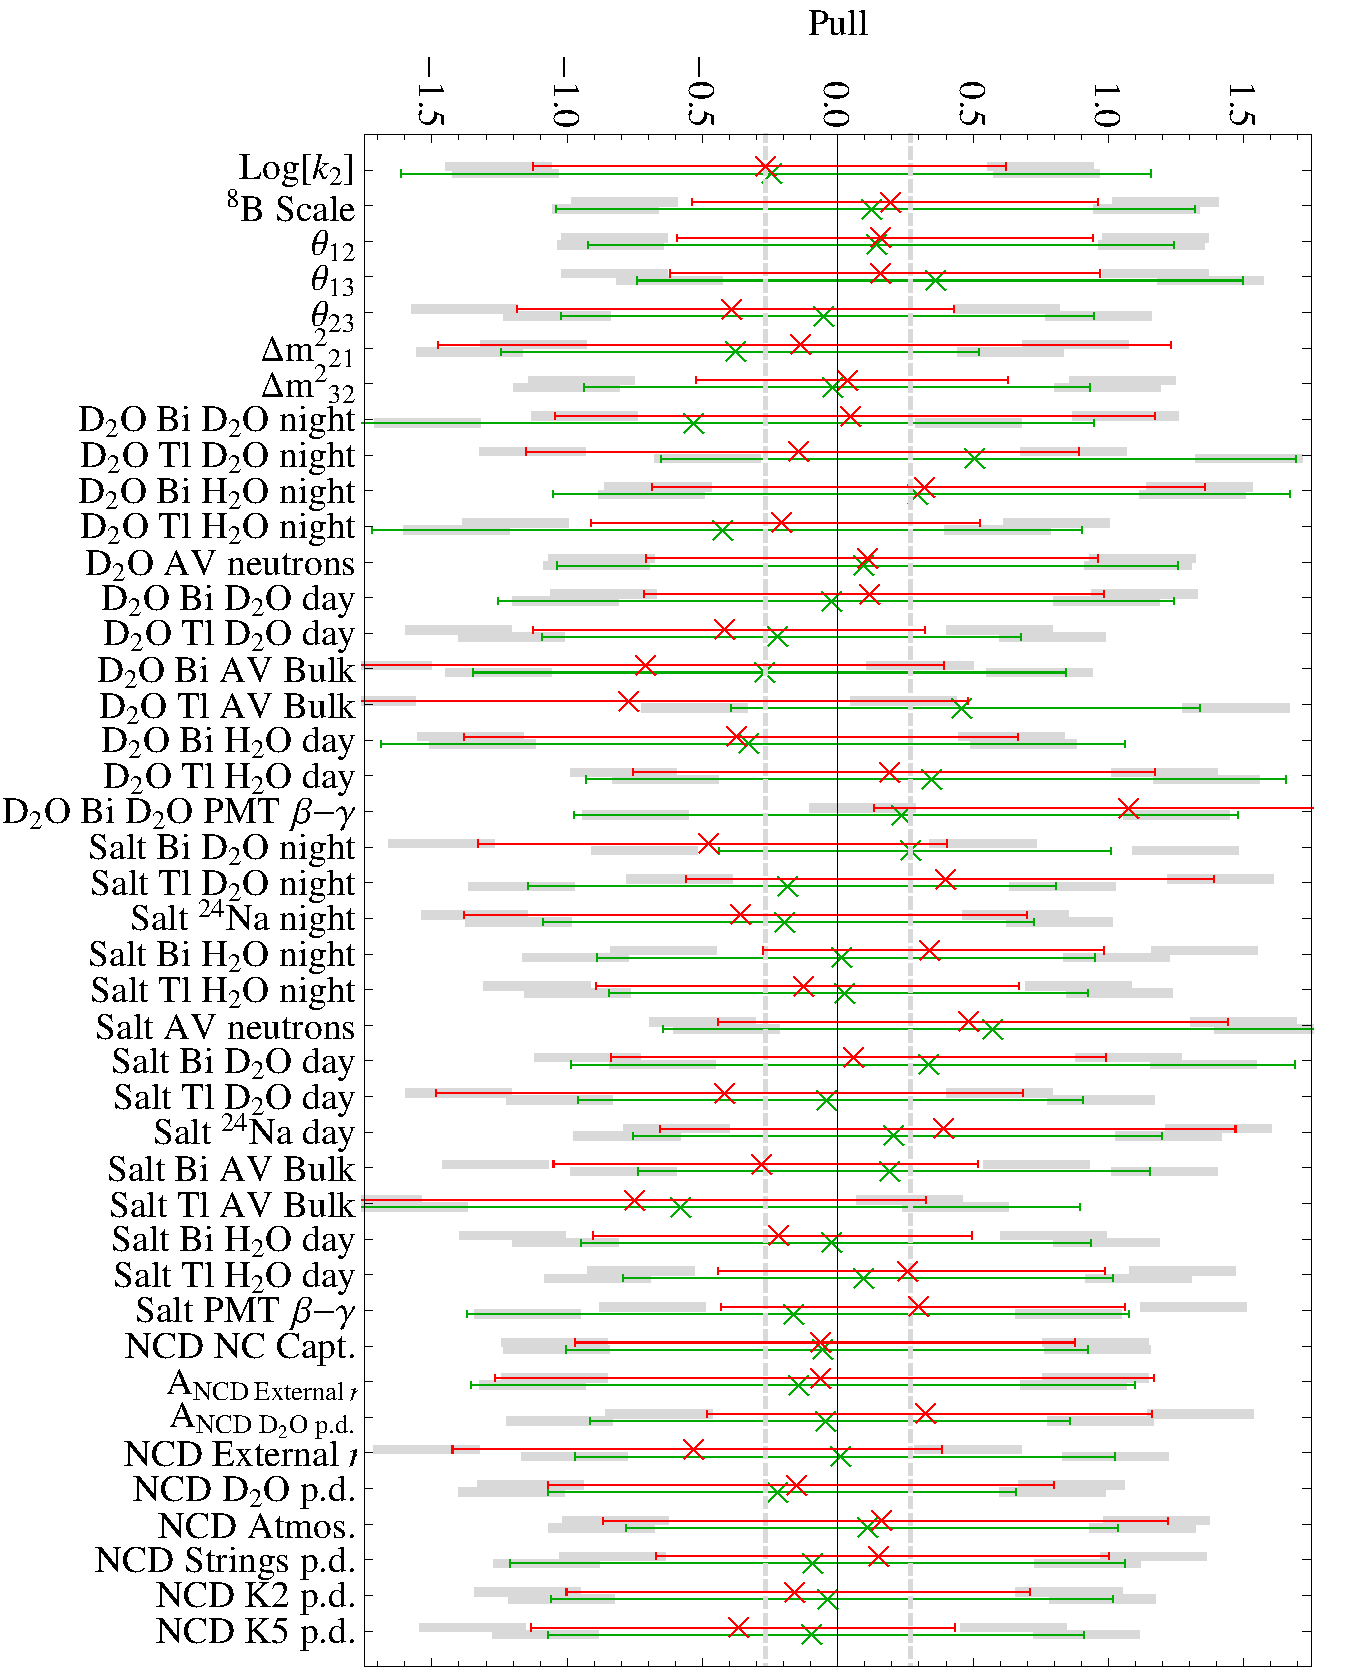
\includegraphics[height=0.85\columnwidth,angle=90]{pull_combined}
\caption{
The pull of all fitted parameters with signal + all backgrounds datasets. Gray bars and dashed lines represent expected fluctuations due to limited statistics. The alternate ensemble results are shown in green for comparison.
}
\label{fig:allbg_pull}
\end{figure}

\begin{figure}
\centering
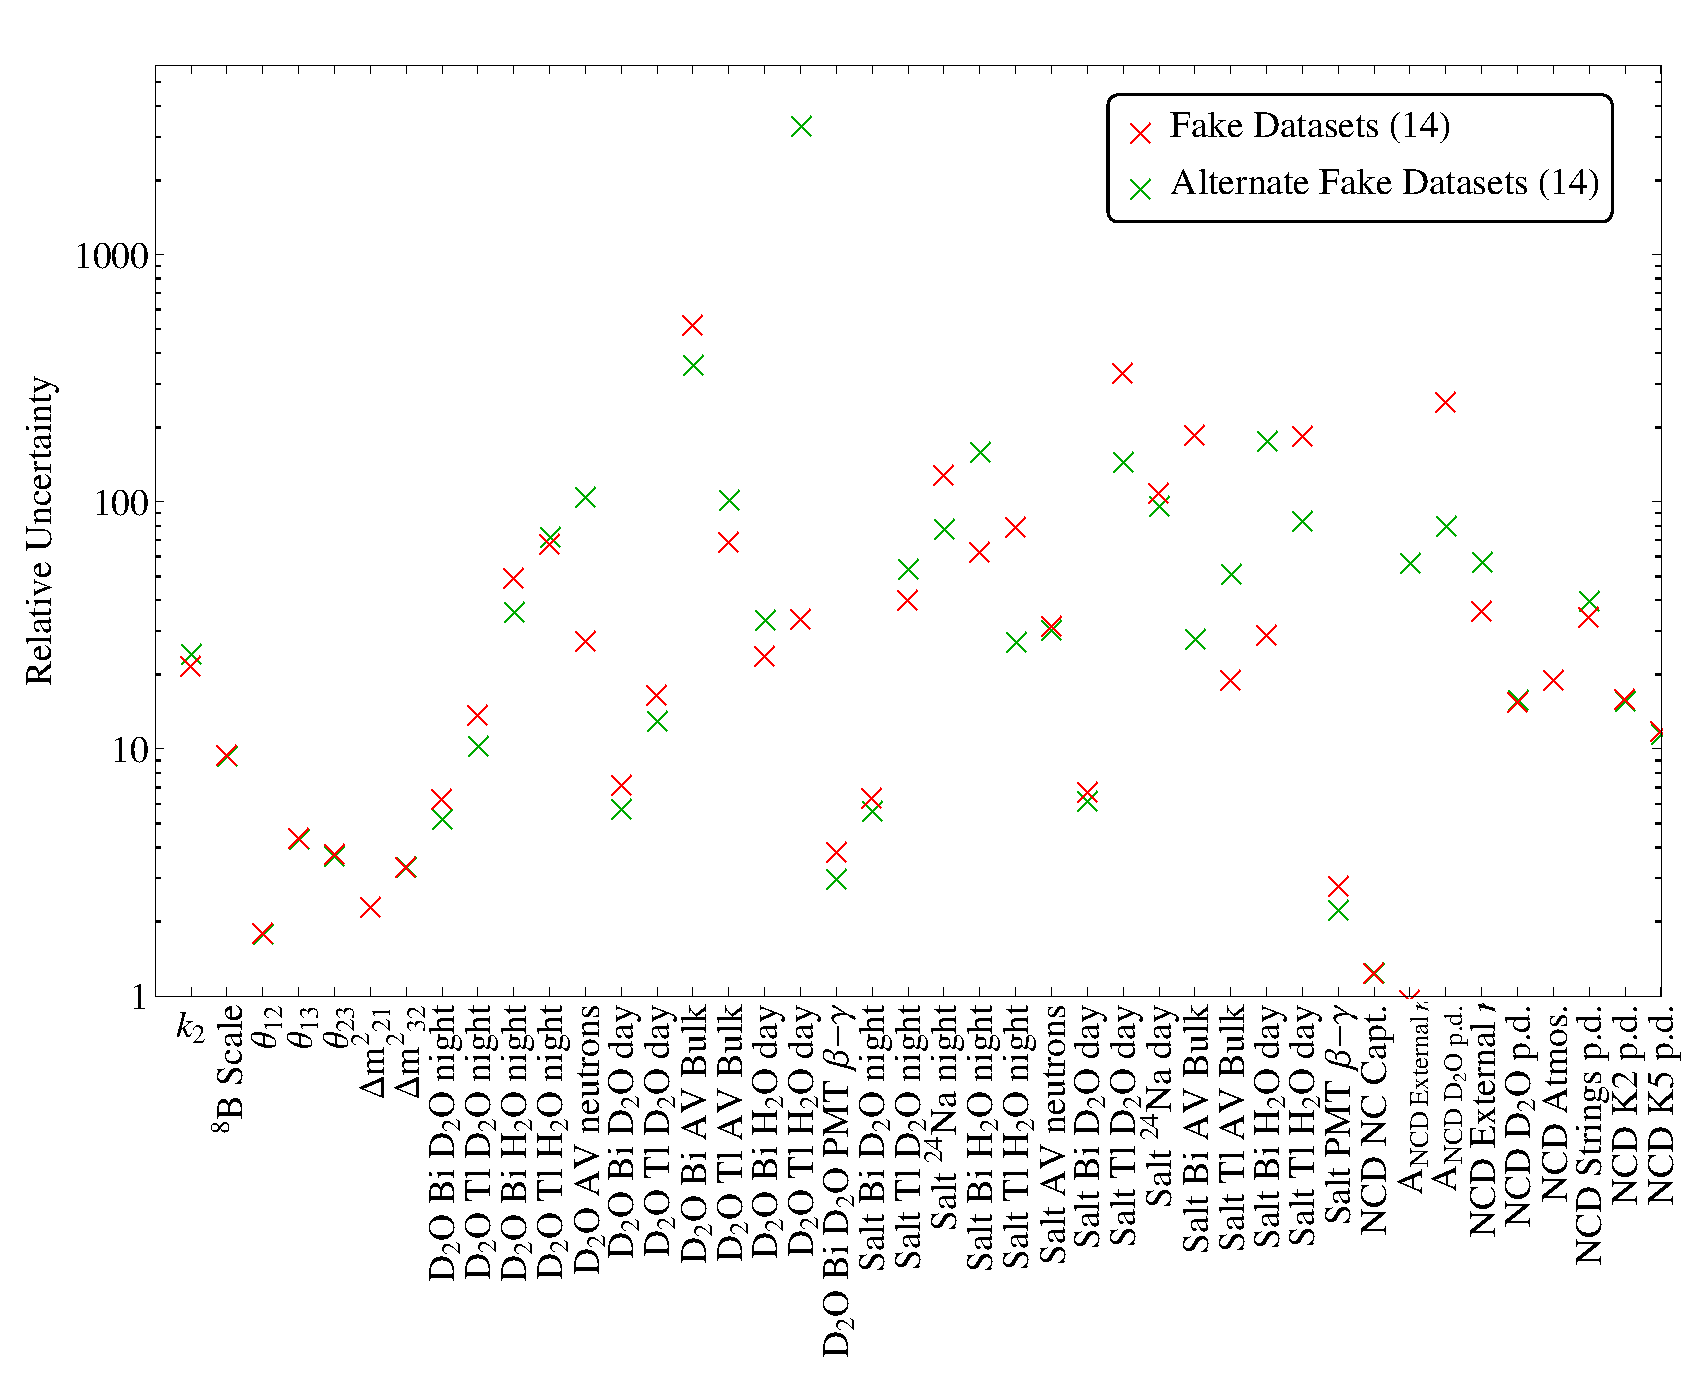
\includegraphics[height=0.85\columnwidth,angle=90]{reluncert_combined}
\caption{
The relative uncertainty of all fitted parameters with signal + all backgrounds datasets. The alternate ensemble results are shown in green for comparison.
}
\label{fig:allbg_reluncert}
\end{figure}

\clearpage

\subsection{Independent Impact of Systematics}

The following systematic tests were done at the best fit values for a fake dataset of comparable statistics to the SNO 3-phase dataset with all backgrounds included. 
This fake dataset was seeded with $k_2 = 10^{-4}$~s/eV and had the $^8$B flux seeded and fixed at the SSM central value.
The parameters considered here include all parameters whose uncertainties are propagated with the shift-and-refit method. 
\Cref{fig:detector_systematics1,fig:detector_systematics2} show the individual contributions of these parameters independently.
In the final fit these systematics will be propagated by simultaneously shifting all parameters and refitting as described in \Cref{systematics}, however, for this test it was desired to know the impact of each parameter.
When summed in quadrature, the total uncertainty on $k_2$ is found to be $^{+13.4\%}_{-9.03\%}$.

\begin{figure}
\centering
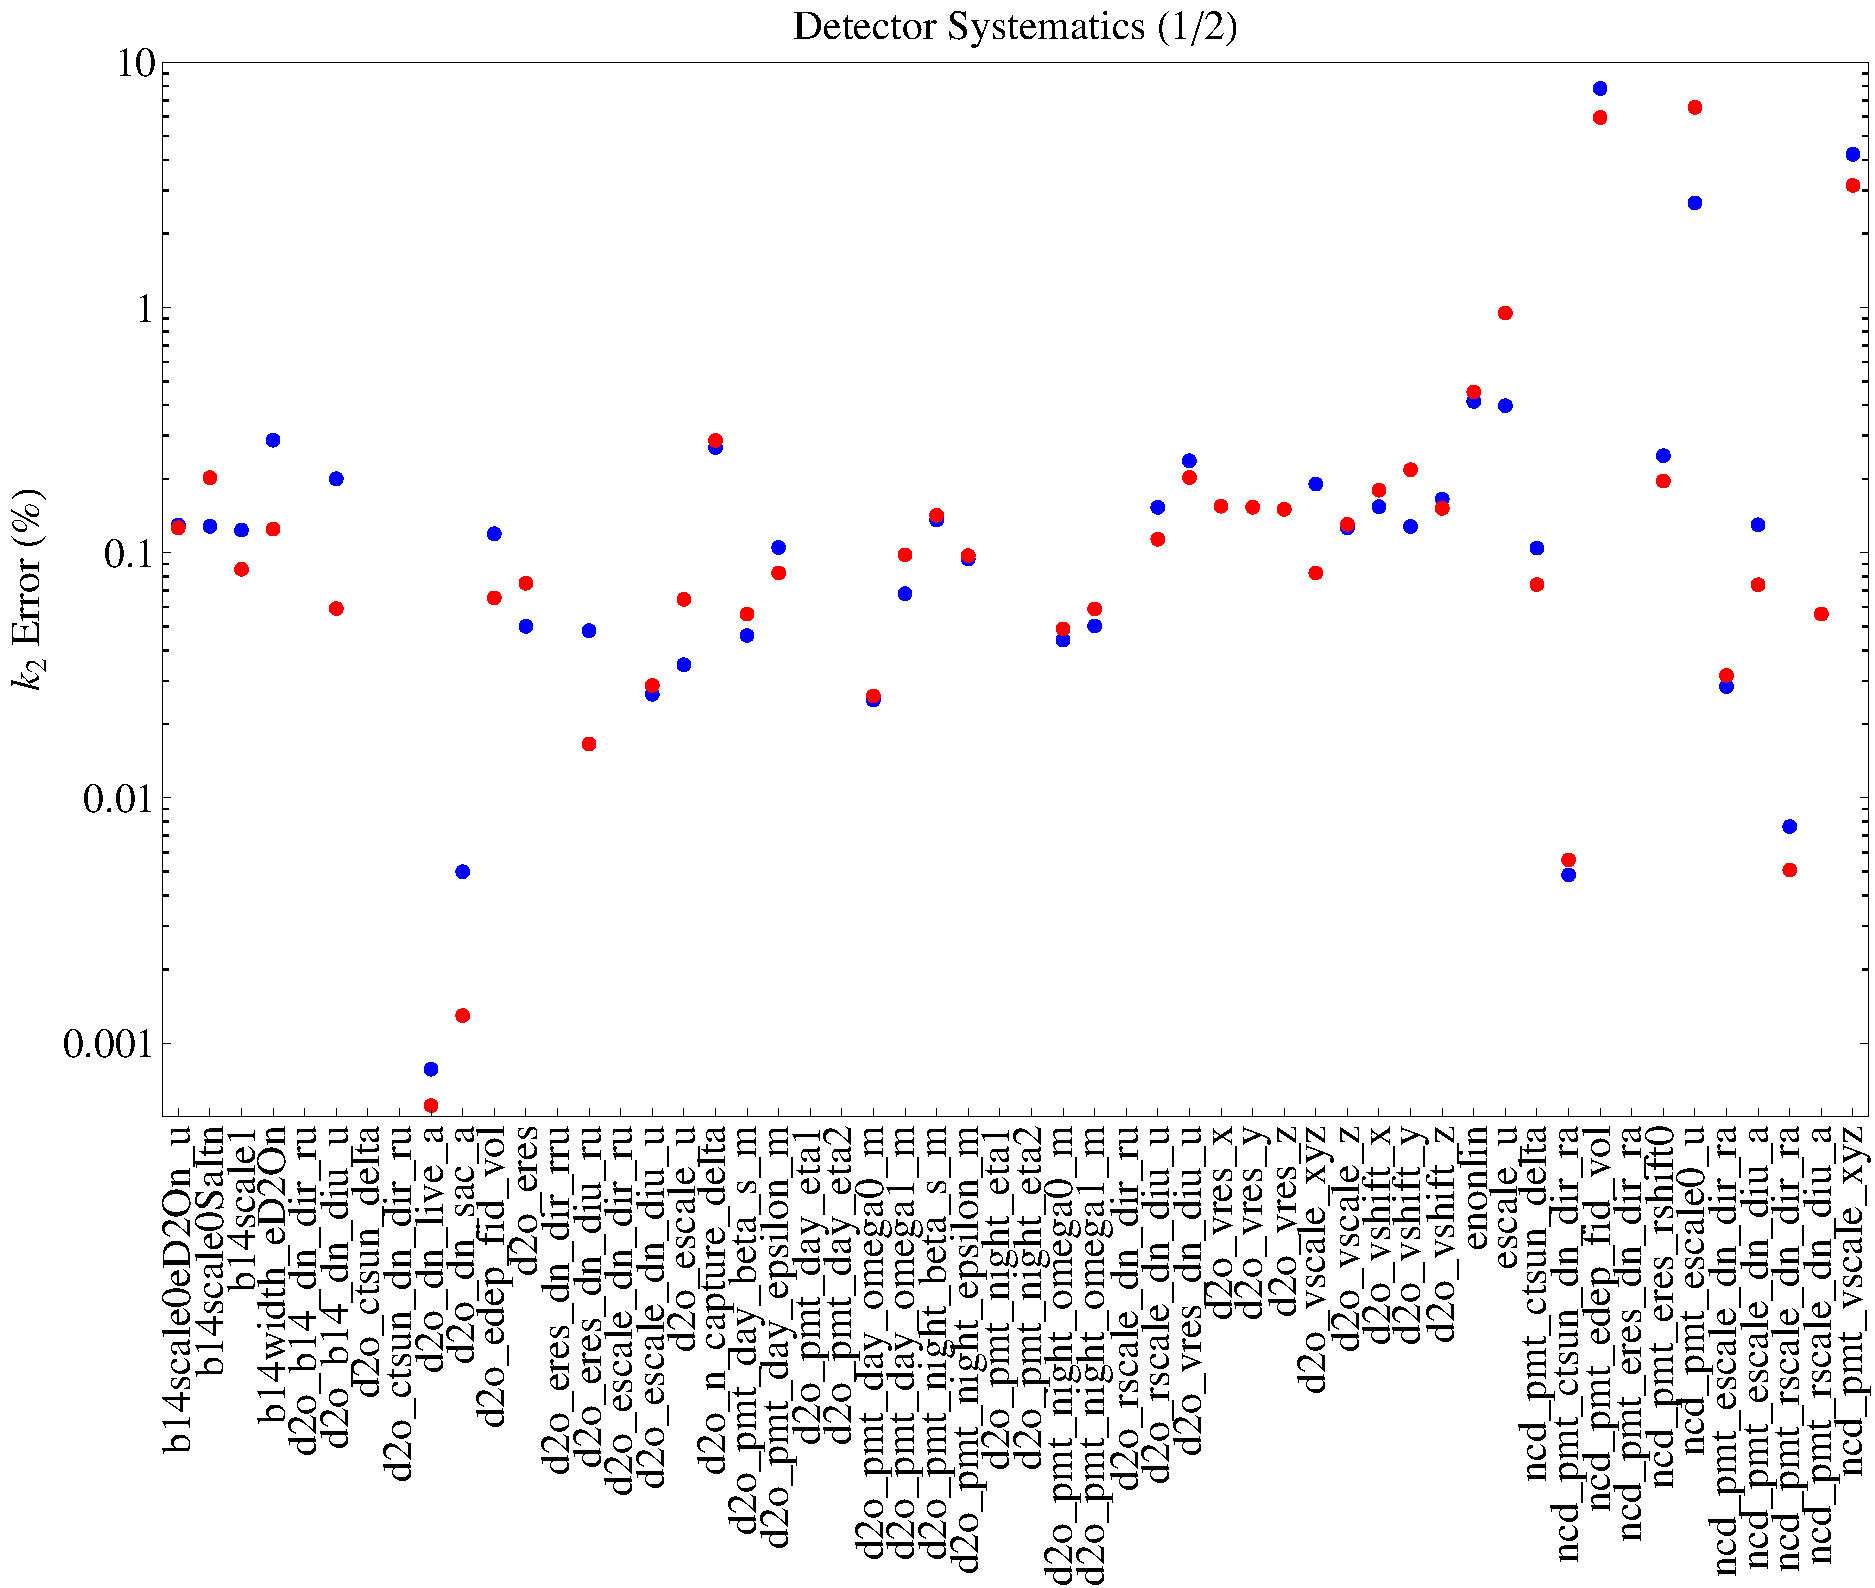
\includegraphics[width=0.85\columnwidth]{basic_1_2}
\caption{The calculated systematic effect on $k_2$ from the first half of the detector systematic parameters in the fit is shown here. Red represents positive (blue, negative) fractional error.}
\label{fig:detector_systematics1}
\end{figure}

\begin{figure}
\centering
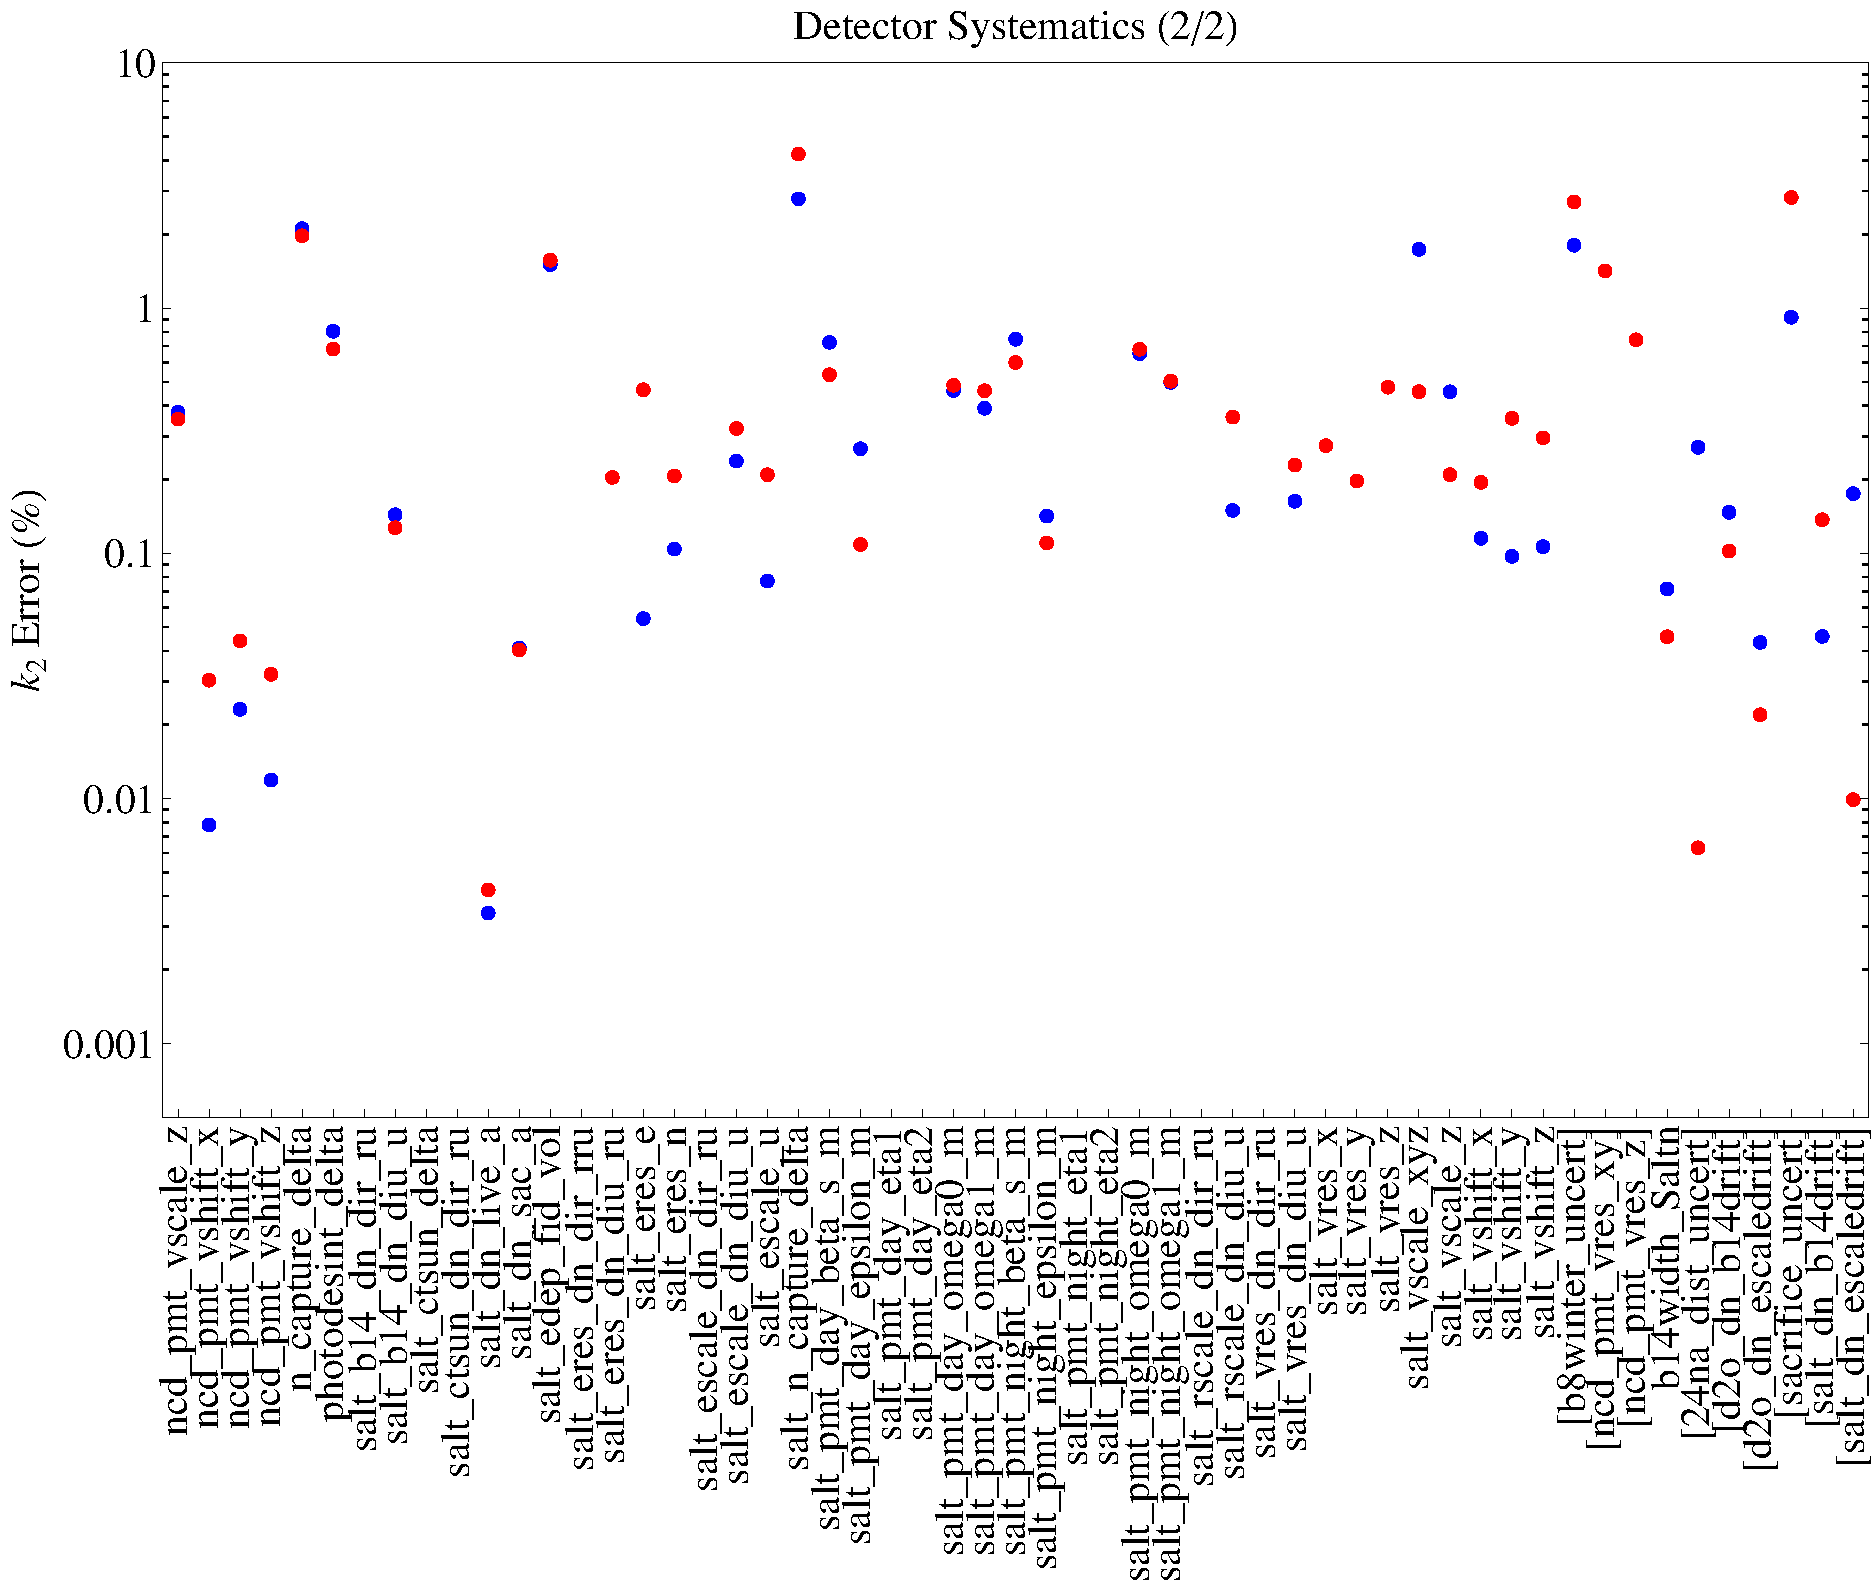
\includegraphics[width=0.85\columnwidth]{basic_2_2}
\caption{The calculated systematic effect on $k_2$ from the second half of the detector systematic parameters in the fit is shown here. Red represents positive (blue, negative) fractional error.}
\label{fig:detector_systematics2}
\end{figure}


\clearpage 

\section{\texorpdfstring{\nicefrac{1}{3}}{1/3} Dataset}
\label{third}

Using 1/3 of the SNO dataset --- the same 1/3 dataset used in testing the historical 3-phase fits --- the fit was run as described in \Cref{strategy}. 
To reduce computational power required for this test, the central values of scanned nuisance parameters from the 3-phase Pee+Pea fit~\cite{3phase} were used. 
These are nominally uncorrelated with neutrino parameters, and would take a very long time to iteratively scan with little gain.
This scan will, of course, be done for the full dataset.
The scan of $k_2$ and the $^8$B flux are shown in \Cref{fig:third_scans}.
The neutrino parameters are shown relative to their priors in \Cref{fig:priors_third}.
The observable projections for the minimum and with $k_2$ fixed to infinity are shown in \Cref{third_observables}.

There is a 1-sigma minimum for $k_2$ at a central value of of $4.62\times10^{-4}$~s/eV.
This minimum is almost consistent with infinite lifetime at the one sigma level, and has a one sigma lower bound of $2.40\times10^{-4}$~s/eV.
The fitted value of the $^8$B flux is $5.77^{+0.58}_{-0.58}\times10^6$~cm$^{-2}$s$^{-1}$ ($1.01\pm0.10 \times \Phi_{8B_{BS05(OP)}}$), which is quite consistent with the SSM predictions.
With $k_2$ fixed at infinity the $^8$B flux fits to $5.19^{+0.16}_{-0.16}\times10^6$~cm$^{-2}$s$^{-1}$ ($0.91\pm0.03 \times \Phi_{8B_{BS05(OP)}}$).
Both flux measurements are consistent with previous 3-phase SNO results: $5.23^{+0.16}_{-0.16}\times10^6$~cm$^{-2}$s$^{-1}$ ($0.92\pm0.03 \times \Phi_{8B_{BS05(OP)}}$).

\begin{figure}
\centering
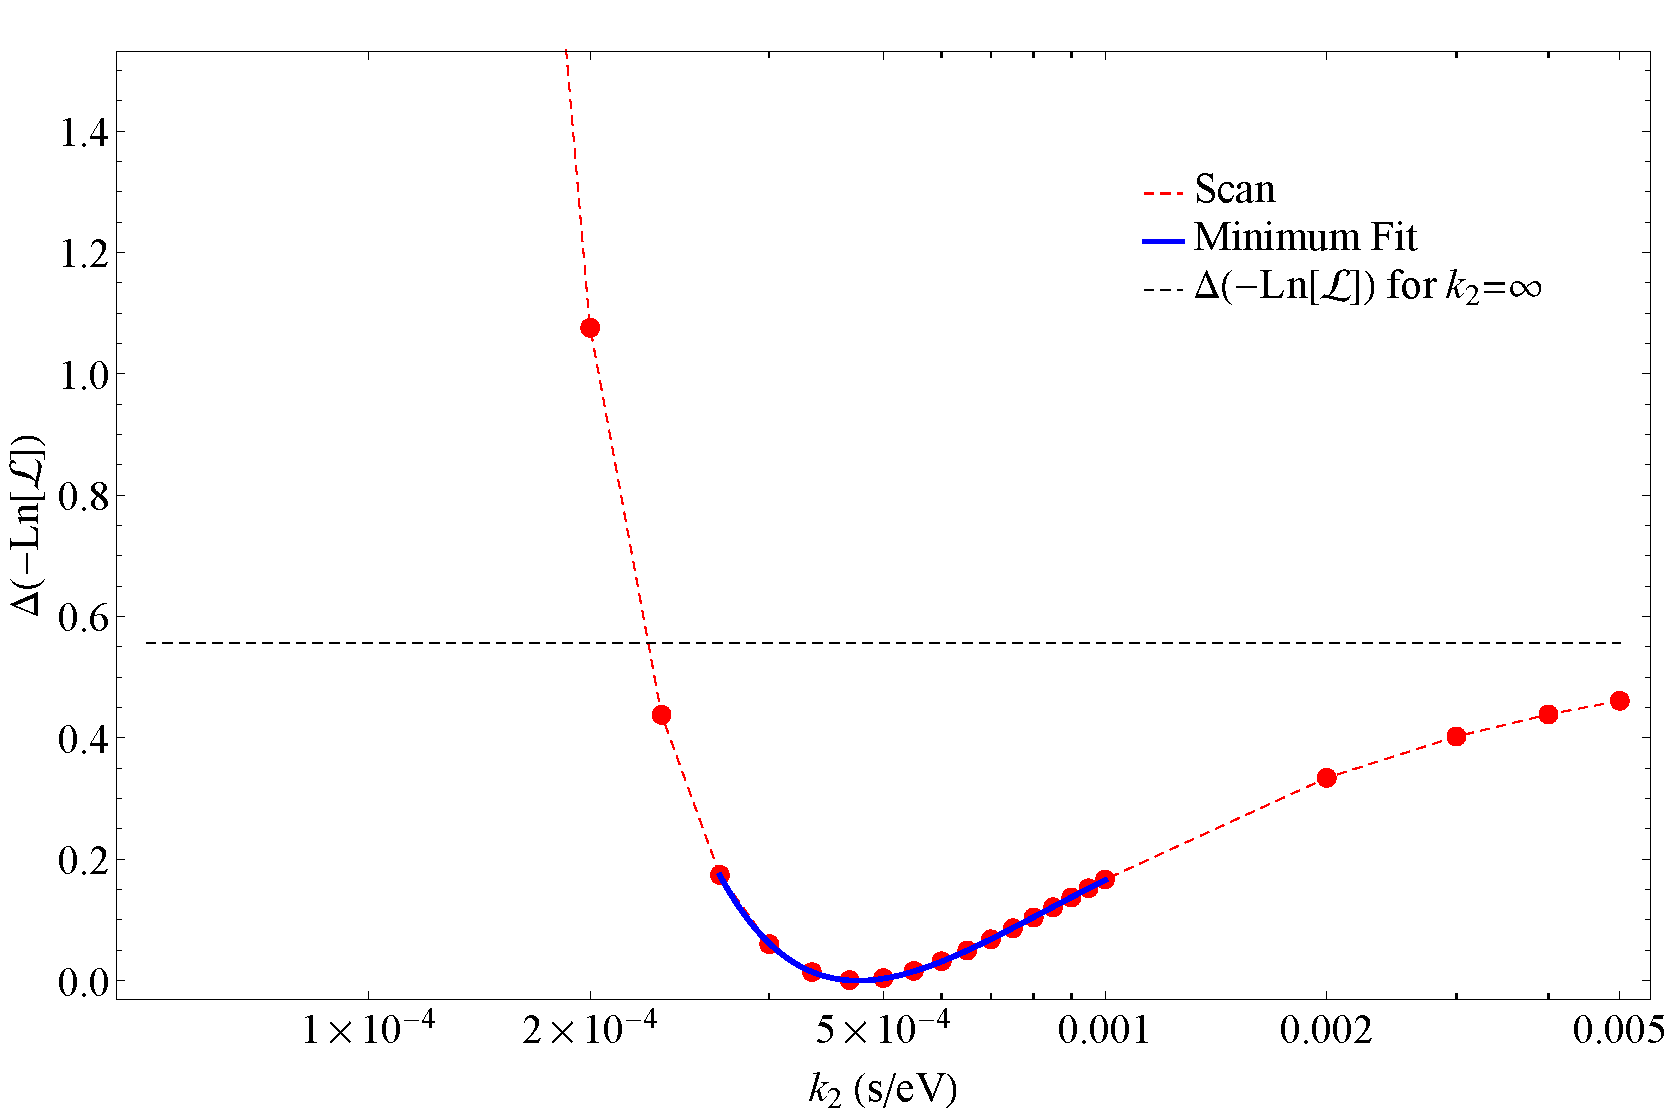
\includegraphics[width=0.85\columnwidth]{k2_scan_third} \\
\vspace{12pt}
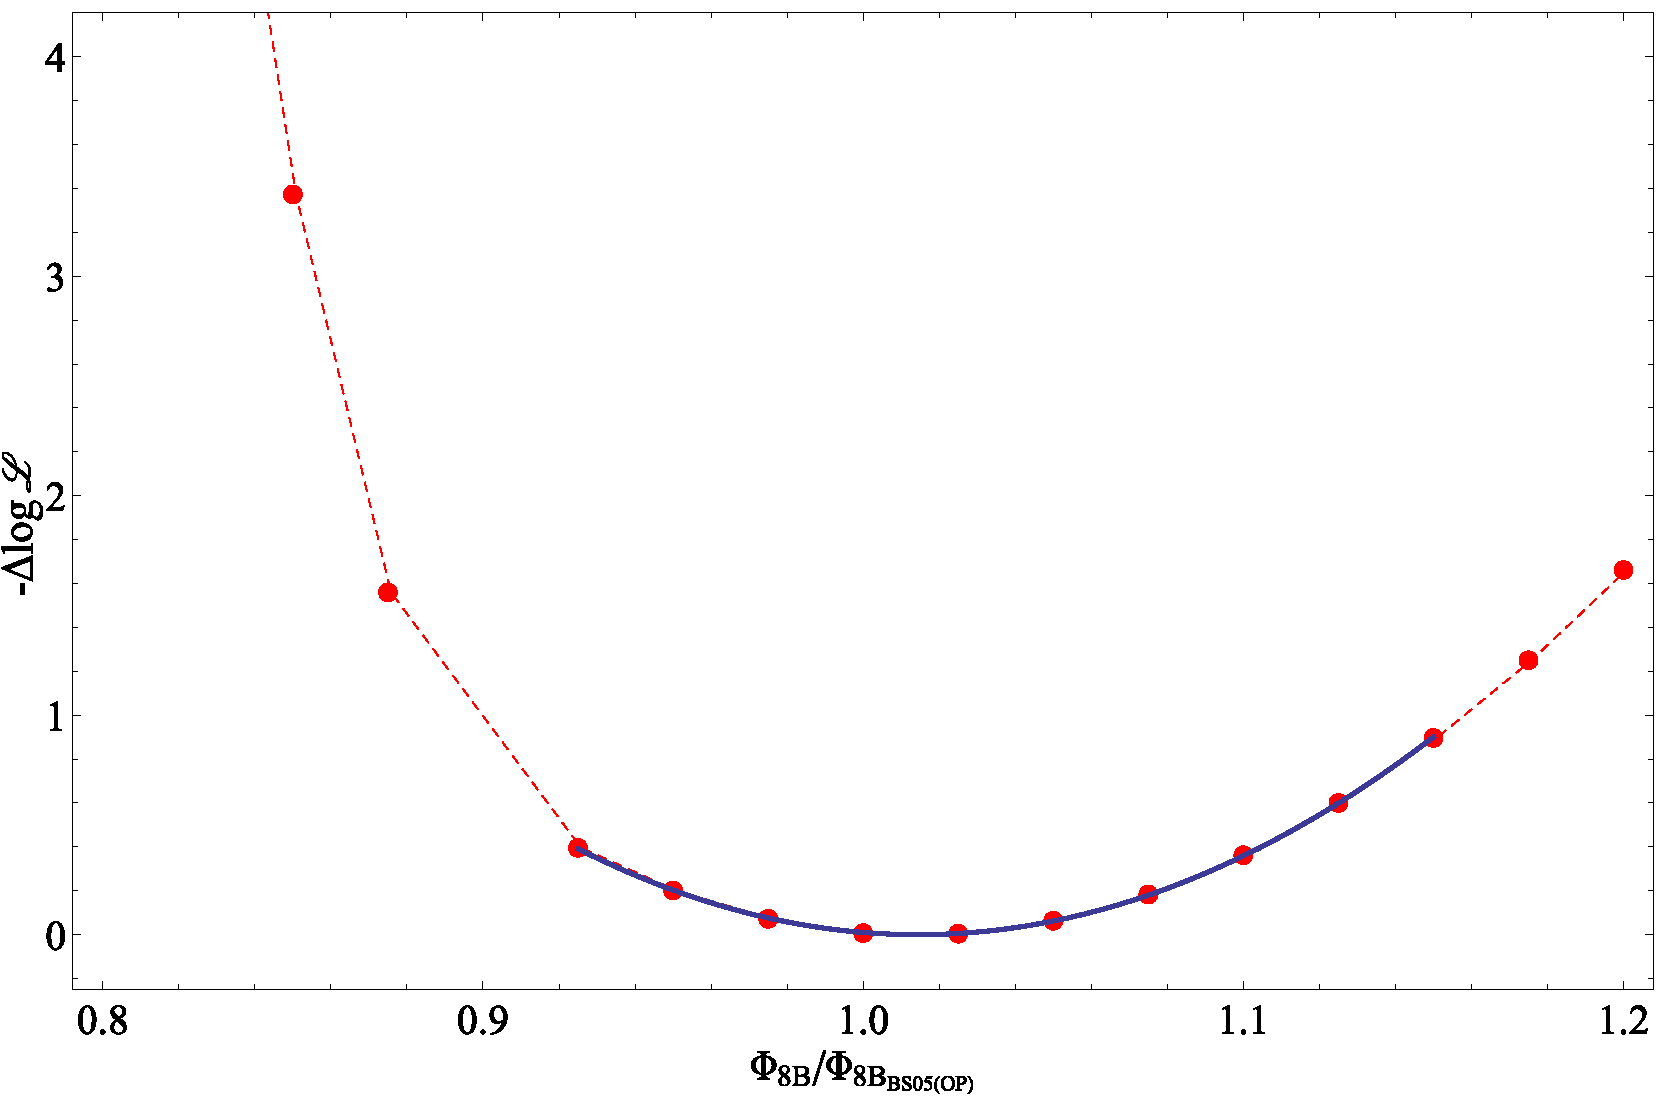
\includegraphics[width=0.85\columnwidth]{flux_scan_third}
\caption{The scans of $k_2$ and the $^8$B flux for the 1/3 dataset. The red points are the scan values, and the blue line is a fit to the minimum.}
\label{fig:third_scans}
\end{figure}

\begin{figure}
\centering
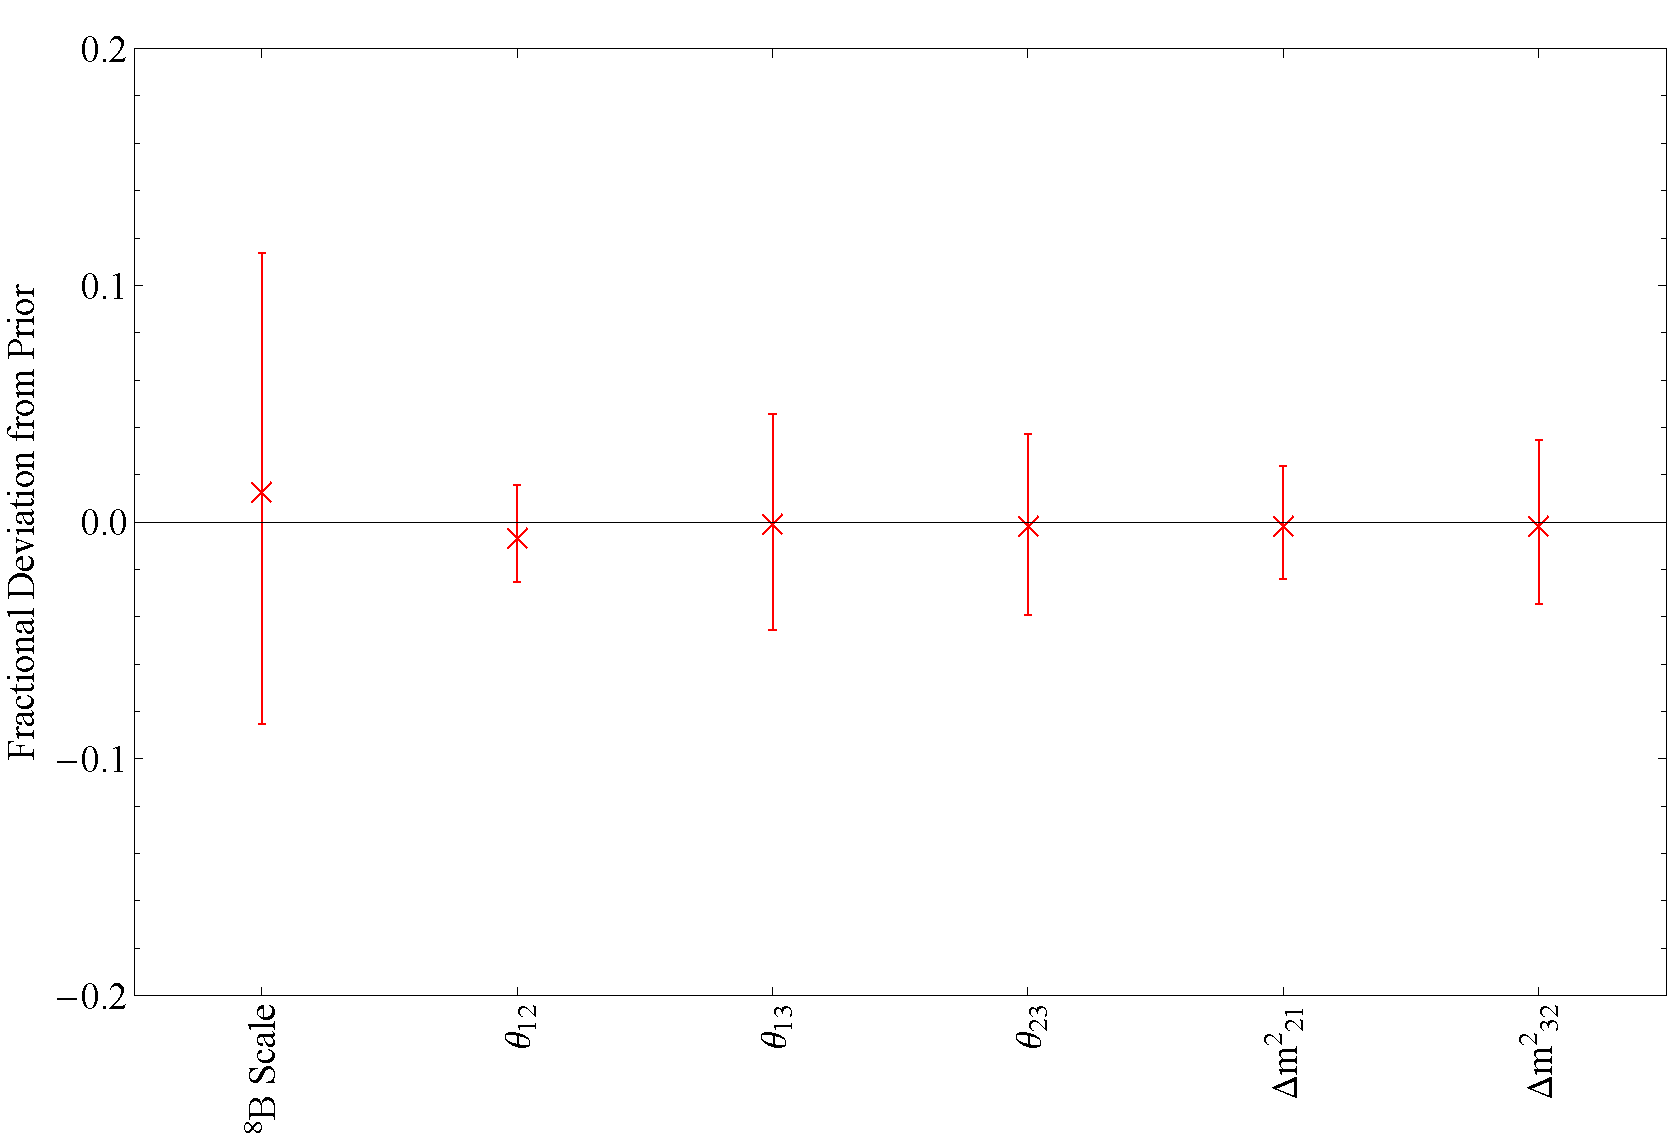
\includegraphics[width=0.85\columnwidth]{prior_deviation_third}
\caption{The fractional deviation of each neutrino parameter with a prior constraint from its prior. The errors shown are the fractional errors of the fit.}
\label{fig:priors_third}
\end{figure}

\clearpage

\section{Final Results}
\label{final}

Now with the entire SNO dataset, the fit was run as described in \Cref{strategy}. 
As a preliminary step, the systematics identified in the previous 3-phase analysis as requiring scanning were scanned iteratively until a global minimum was found.
Using the central values for the systematics, both $k_2$ and $^8$B flux were then scanned with the systematic parameters fixed at their central values, and are shown in \Cref{fig:final_scans}.
The neutrino parameters are shown relative to their priors at the minimum of this scan in \Cref{fig:priors_final}.
The observable projections for the minimum and with $k_2$ fixed to infinity are shown in \Cref{final_observables}.
The likelihood profile including systematic uncertainties is compared to the likelihood profile without systematics in \Cref{fig:systematic_scans}.

The minimum for $k_2$ observed in the 1/3 data fit is still present in this fit (at higher significance) at a central value of of $3.45^{+5.50}_{-1.68}\times10^{-4}$~s/eV where the uncertainty given is the total uncertainty.
This minimum is consistent with infinite lifetime at a bit over $85\%$ confidence, and sets a $90\%$ confidence lower bound at $>8.08\times10^{-5}$~s/eV.
This lower bound was found by applying Wilks' theorem to the systematically broadened likelihood, i.e. when the $-2\Delta\log{L}$ from the minimum crosses $2.71$.
The fitted value of the $^8$B flux is $6.08^{+0.47}_{-0.47}$(stat.)$^{+0.21}_{-0.22}$(syst.)$\times10^6$~cm$^{-2}$s$^{-1}$ ($1.07\pm0.10 \times \Phi_{8B_{BS05(OP)}}$), which is quite consistent with the SSM predictions and constraint.
With $k_2$ fixed at infinity the $^8$B flux fits to $5.22^{+0.16}_{-0.16}\times10^6$~cm$^{-2}$s$^{-1}$ ($0.92\pm0.03 \times \Phi_{8B_{BS05(OP)}}$).
The flux measurement with $k_2$ fixed at infinity is expected to reproduce previous 3-phase results, and is quite consistent consistent with those results: $5.23^{+0.16}_{-0.16}\times10^6$~cm$^{-2}$s$^{-1}$ ($0.92\pm0.03 \times \Phi_{8B_{BS05(OP)}}$).
There is some tension between the SNO result and the flux fitted with with $k_2$ floating, however, they are consistent at two sigma. 

\begin{figure}
\centering
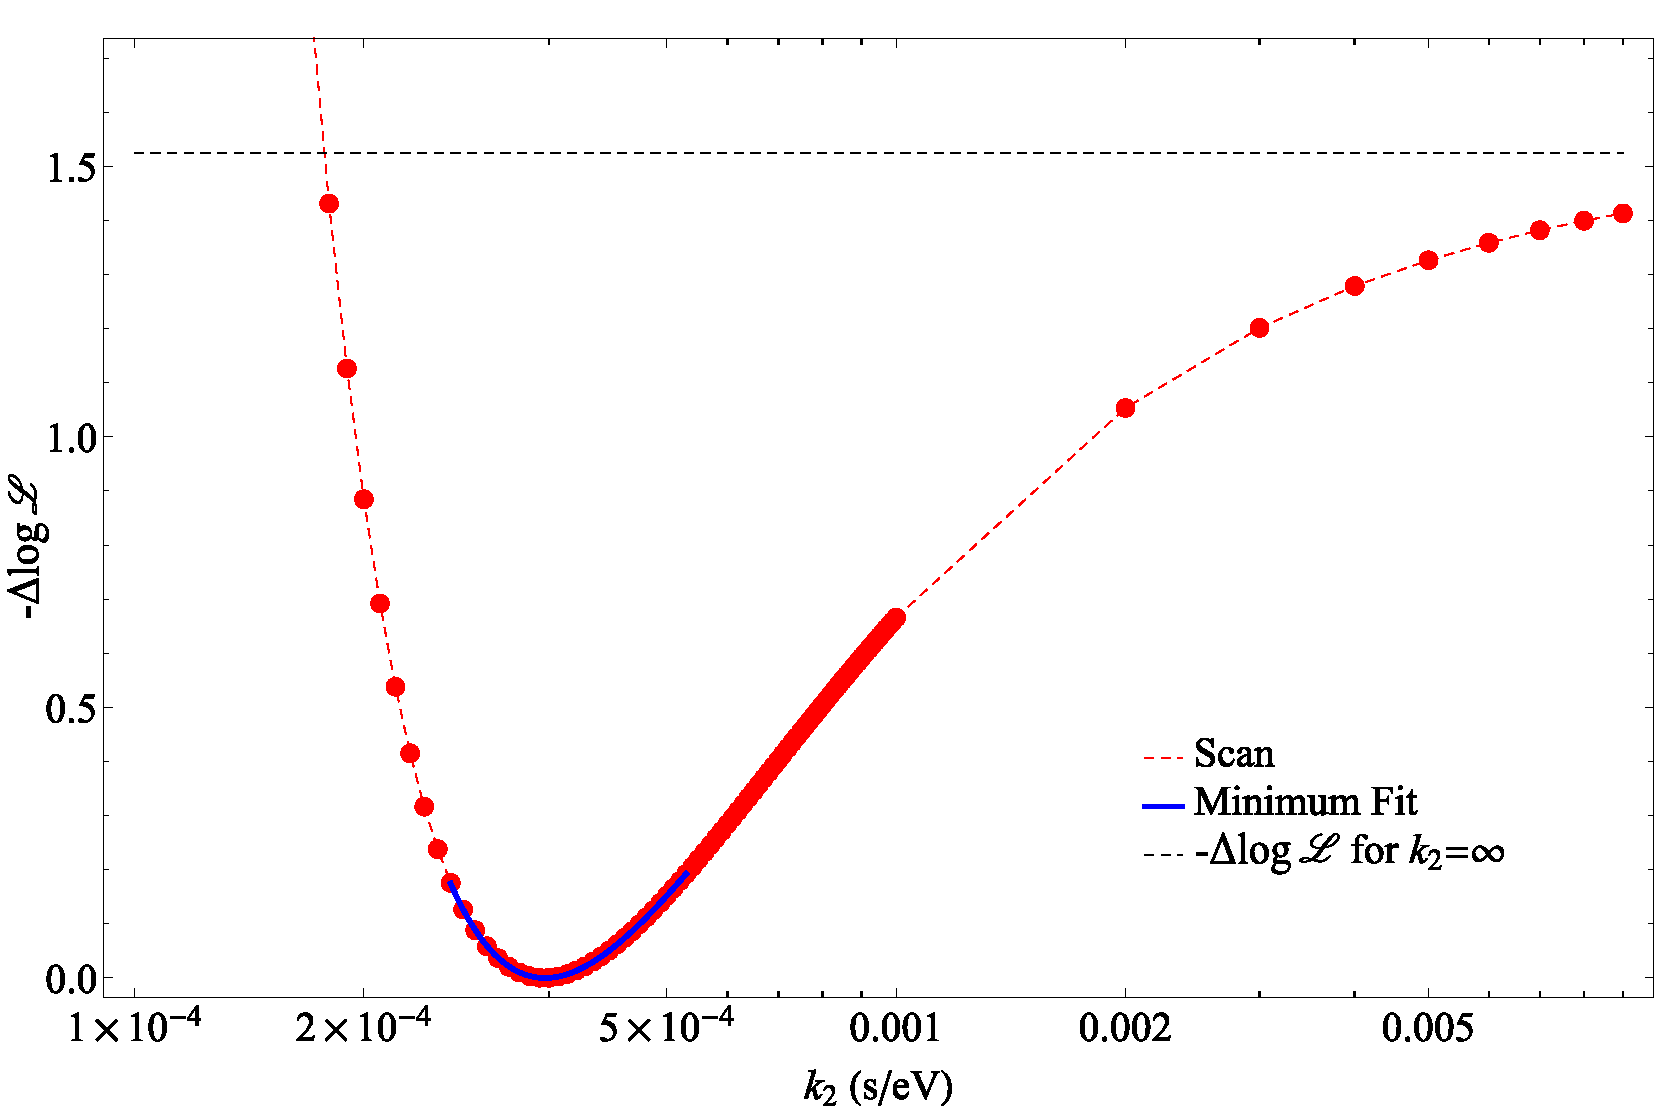
\includegraphics[width=0.85\columnwidth]{k2_scan_final} \\
\vspace{12pt}
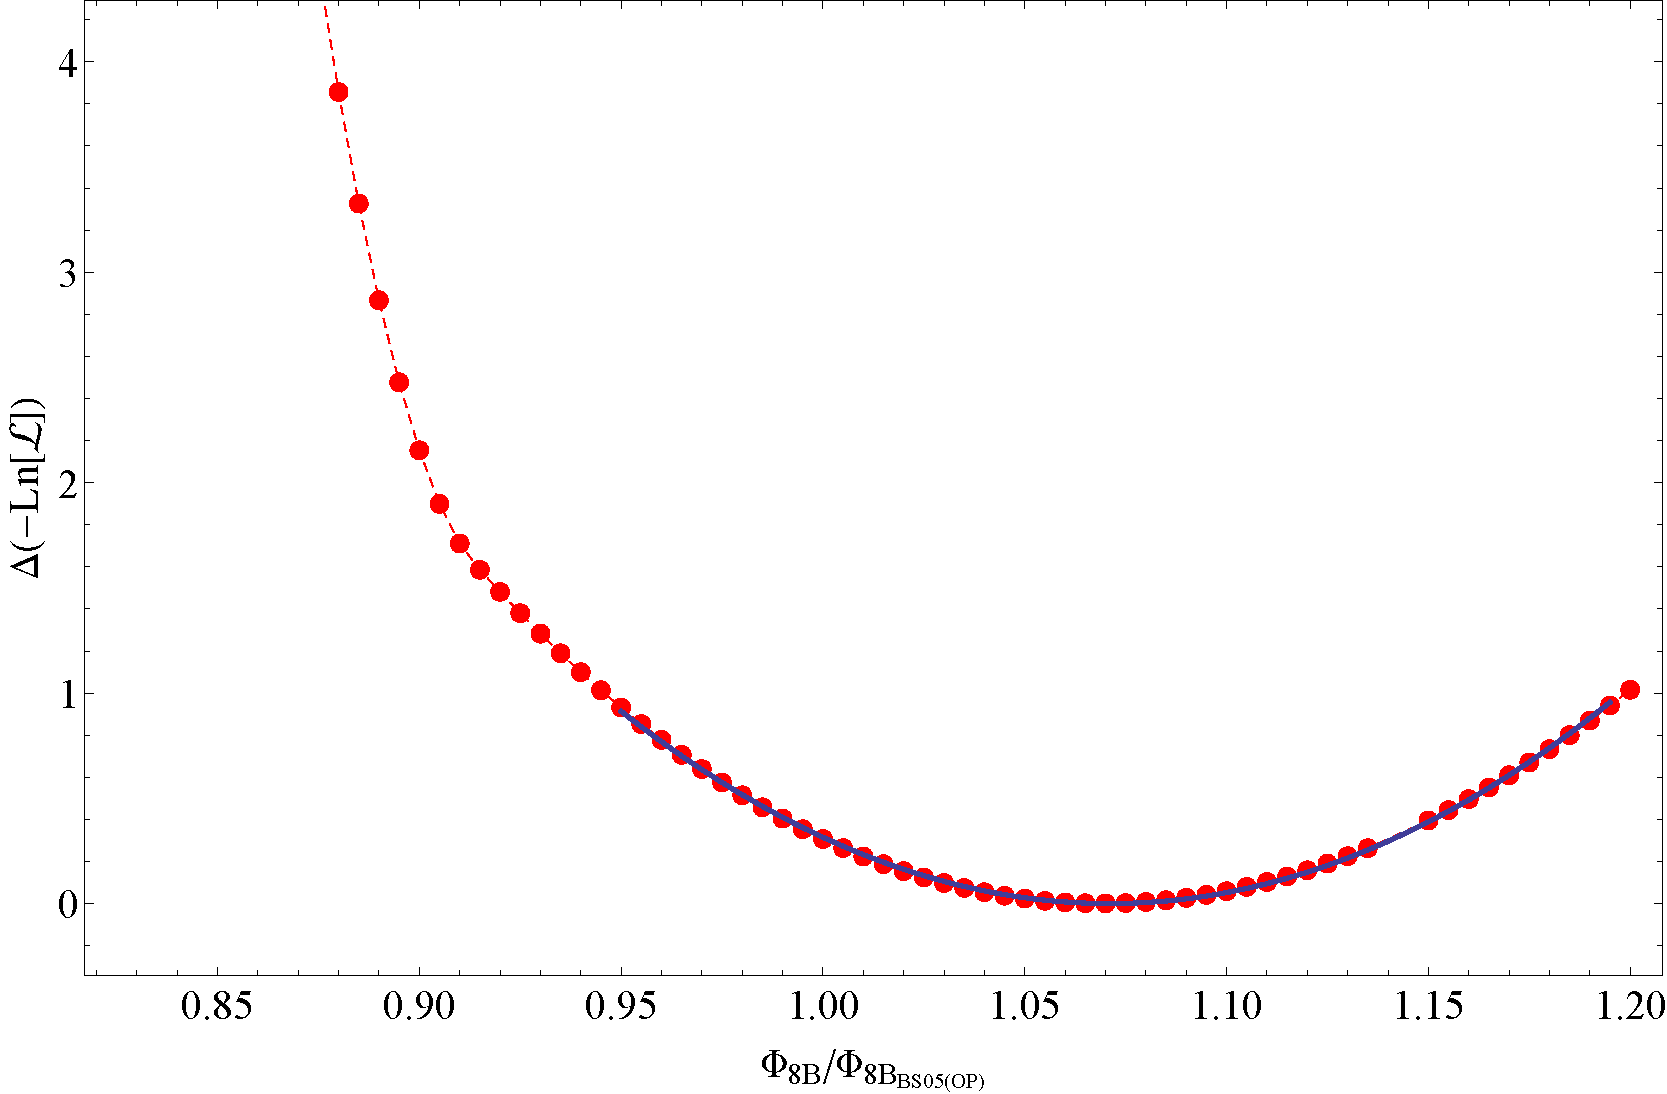
\includegraphics[width=0.85\columnwidth]{flux_scan_final}
\caption{The scans of $k_2$ and the $^8$B flux for the full dataset. The red points are the scan values, and the blue line is a fit to the minimum.}
\label{fig:final_scans}
\end{figure}

\begin{figure}
\centering
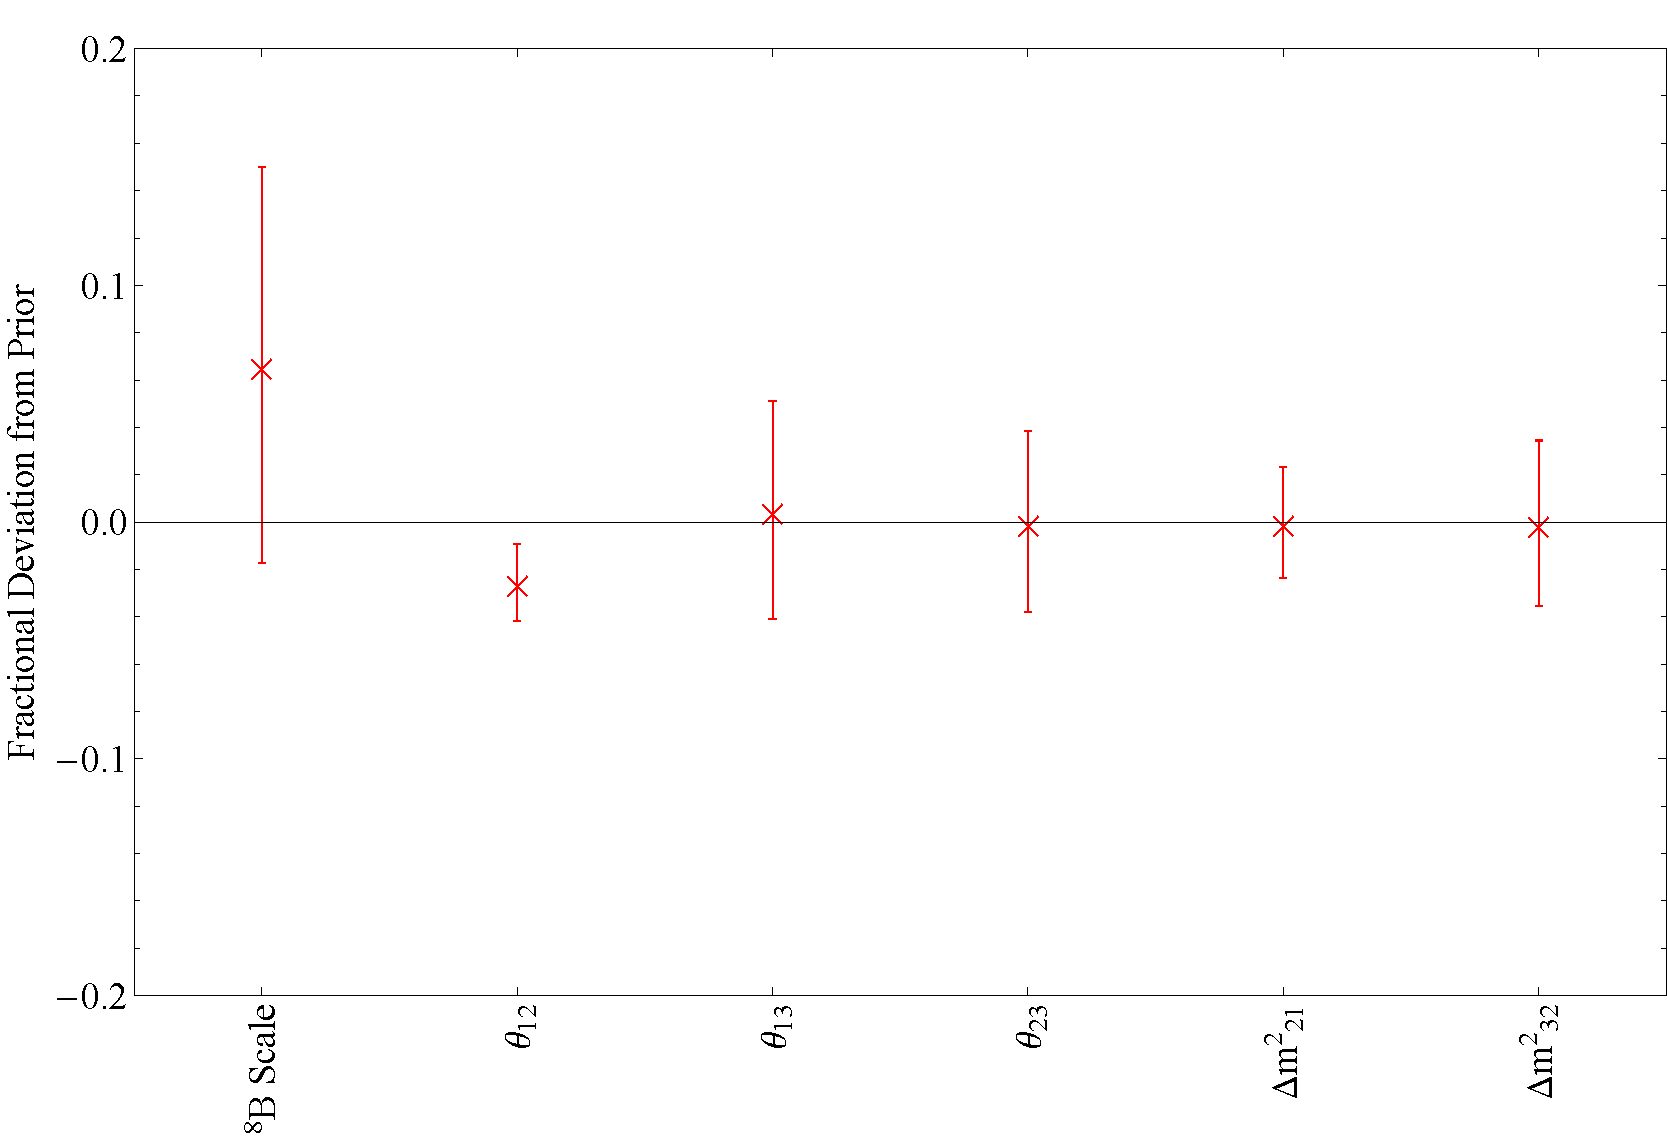
\includegraphics[width=0.85\columnwidth]{prior_deviation_final}
\caption{The fractional deviation of each neutrino parameter with a prior constraint from its prior. The errors shown are the fractional errors of the fit.}
\label{fig:priors_final}
\end{figure}

\begin{figure}
\centering
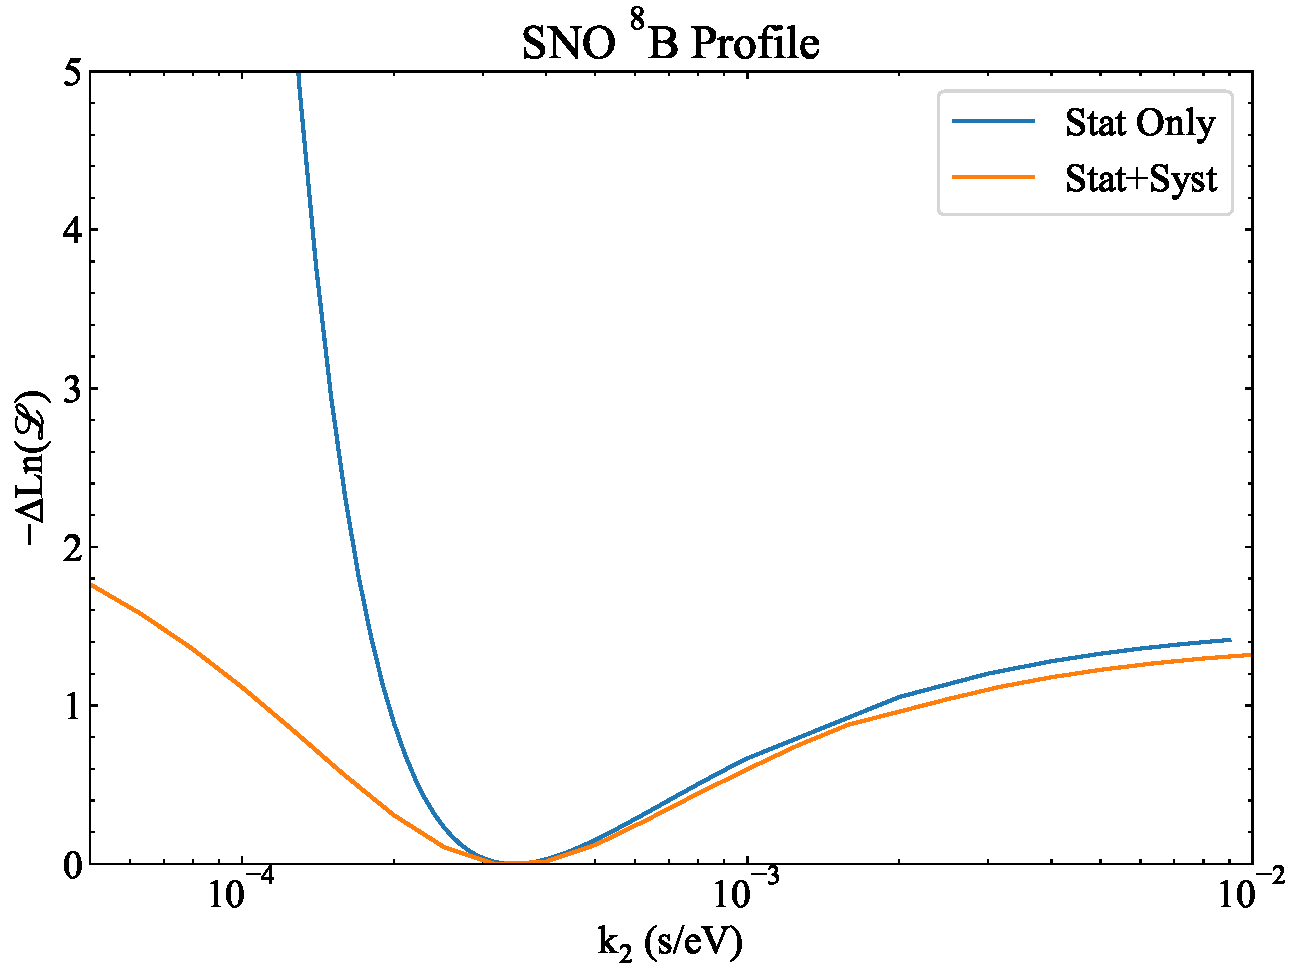
\includegraphics[width=0.85\columnwidth]{sno_8b_stat_syst_profile.pdf}
\caption{The scans of $k_2$ with and without systematic effects. Note that in both cases the minimum has been shifted to zero. With systematics included the minimum is less significant relative to the limiting value at $k_2 \rightarrow \infty$ as expected.}
\label{fig:systematic_scans}
\end{figure}

\clearpage

\section{Global Solar Neutrino Decay Analysis}

The SNO-only $90\%$ confidence lower bound at $>8.08\times10^{-5}$ s/eV from this analysis is not particularly competitive with the best combined analysis~\cite{picoreti}, which sets a $99\%$ confidence lower bound at $>7.2\times10^{-4}$~s/eV (note order of magnitude).
This result was obtained by combining measurements from many solar experiments, and such an analysis can be repeated while including the SNO result described in previous sections.

Experiments have made measurements of solar neutrino interaction rates and published measured fluxes both assuming oscillations (a mixture of neutrino flavors) and no oscillations (assuming a pure electron neutrino flux). 
Practically, the oscillated fluxes are tricky to use because they always depend on a particular set of mixing parameters.
Fortunately, given an unoscillated flux of electron neutrinos, $\Phi_e$, it is straightforward to recover the true neutrino flux, $\Phi_T$ given some oscillation model and knowing the ratio of cross sections for electron $\sigma_e$ and other flavor $\sigma_a$ neutrinos.
\begin{equation}
\Phi_e = (P_{ee} + P_{ea} \frac{\sigma_a}{\sigma_e})\Phi_T
\label{flux_conv}
\end{equation}
The theory described in \Cref{lifetime_model} predicts a value for both $P_{ee}$ and $P_{ea}$ given a set of neutrino mixing parameters, a standard solar model, and a set of neutrino lifetimes.
Since the survival probabilities and cross sections are energy dependent, average quantities weighted by the detected energy spectrum are used.

The total neutrino flux inferred from the survival probability can be directly compared to a standard solar model flux $\Phi_{SSM}$ with a Gaussian constraint term:
\begin{equation}
\mathcal{L} = \frac{(\Phi_T - \Phi_{SSM})^2}{2 \sigma_\Phi^2}
\label{combolike}
\end{equation}
where $\sigma_\Phi$ combines the uncertainty from the measurement with the uncertainty from the SSM.
To account for uncertainties in mixing parameters, these are constrained with similar penalty terms by the same priors from the SNO lifetime analysis (see \Cref{lifetime_model}), and profiled out. 
The lifetime of mass state three is fixed at infinity (solar neutrino fluxes contain negligible amounts of mass state three), while the likelihood is minimized with respect to the lifetime of mass state one where appropriate.

\subsection{\texorpdfstring{$^8$B}{Boron-8} Constraints}

Super-Kamiokande~\cite{superkiv}, KamLAND~\cite{kamland8b} and Borexino~\cite{borexino8b} have all measured the $^8$B neutrino flux via the elastic scatter channel. 
For any particular set of neutrino parameters, the average survival probability values are computed for the elastic scatter cross section weighted energy spectrum of $^8$B neutrinos using the correct production regions (electron density) in the Sun. 
Using these survival probabilities, the measured $\Phi_e$ of each experiment is converted to a true $^8$B flux with \Cref{flux_conv} and compared to the SSM prediction with \Cref{combolike}.
To arrive at a profiled likelihood for each experiment, all neutrino parameters are floated with priors while scanning $k_2$. The lifetime of mass state one is fixed at infinity as with the SNO analysis. 
This produces the profiles in \Cref{fig:8b_profiles}.

\begin{figure}
\centering
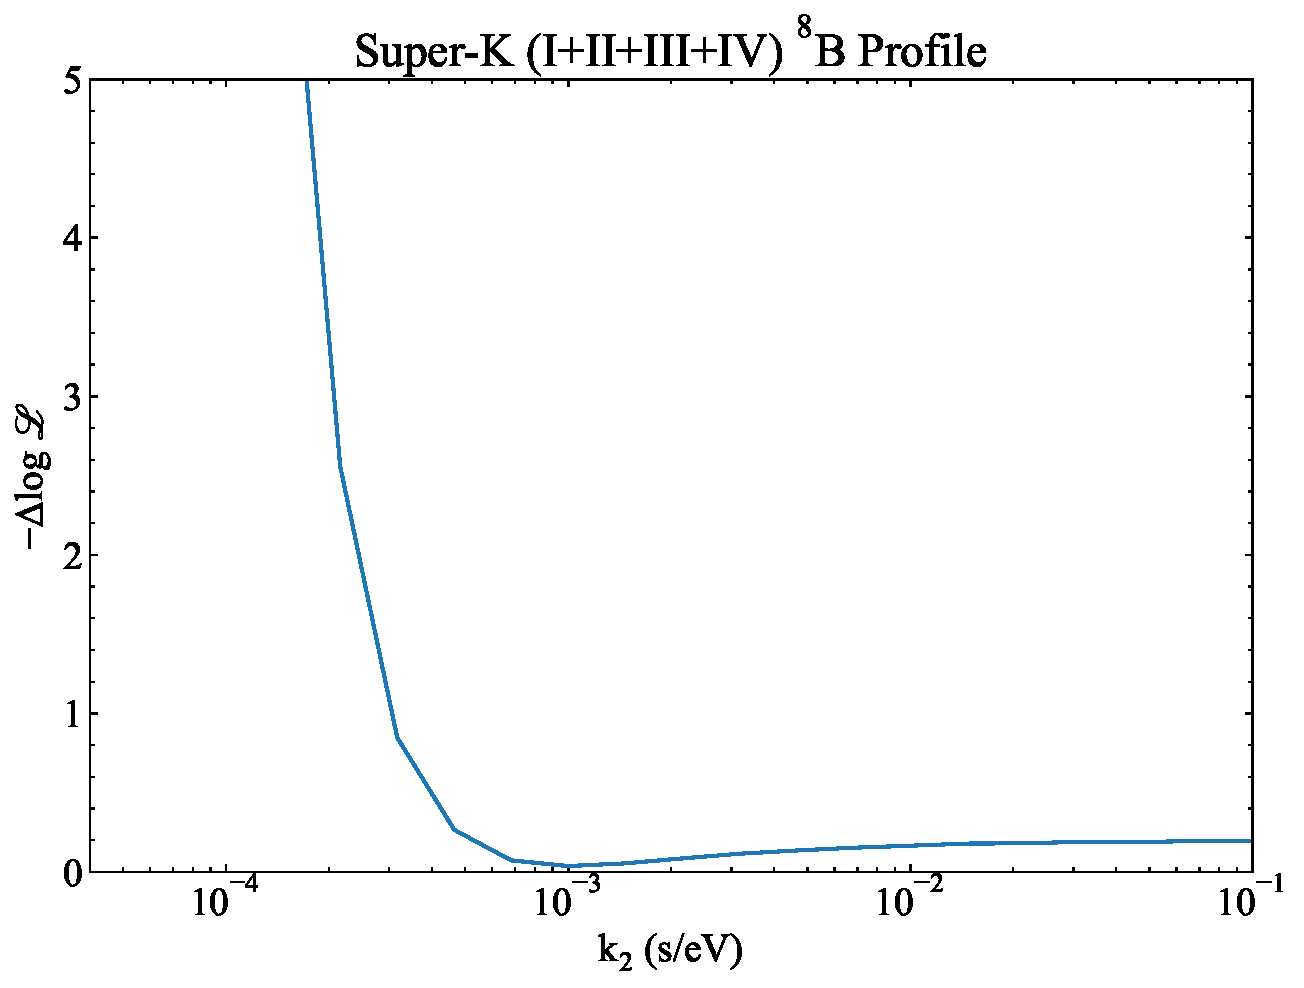
\includegraphics[width=0.5\columnwidth]{superk_8b}
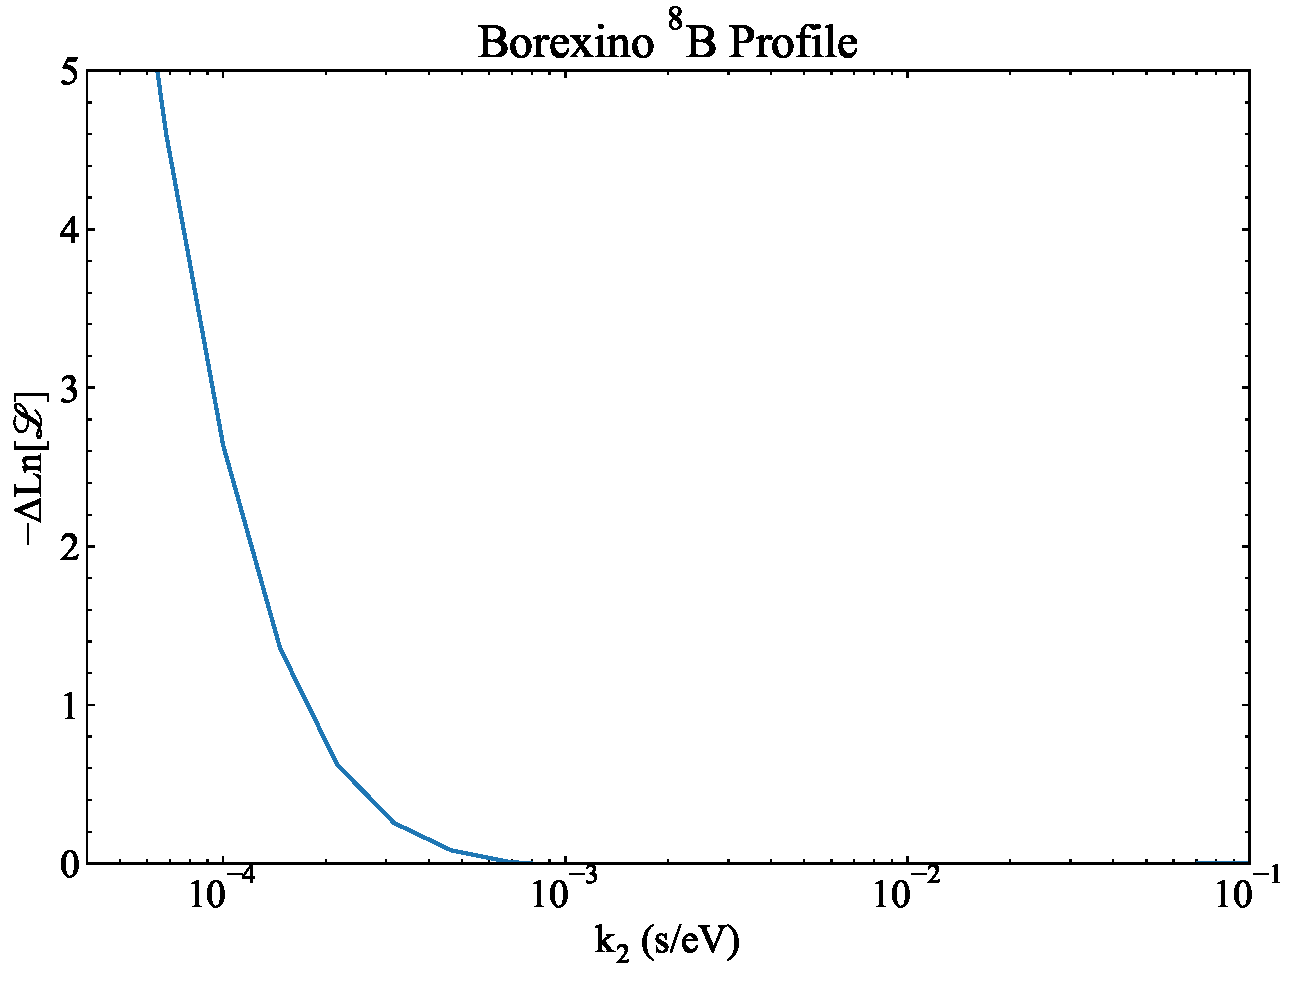
\includegraphics[width=0.5\columnwidth]{borexino_8b}
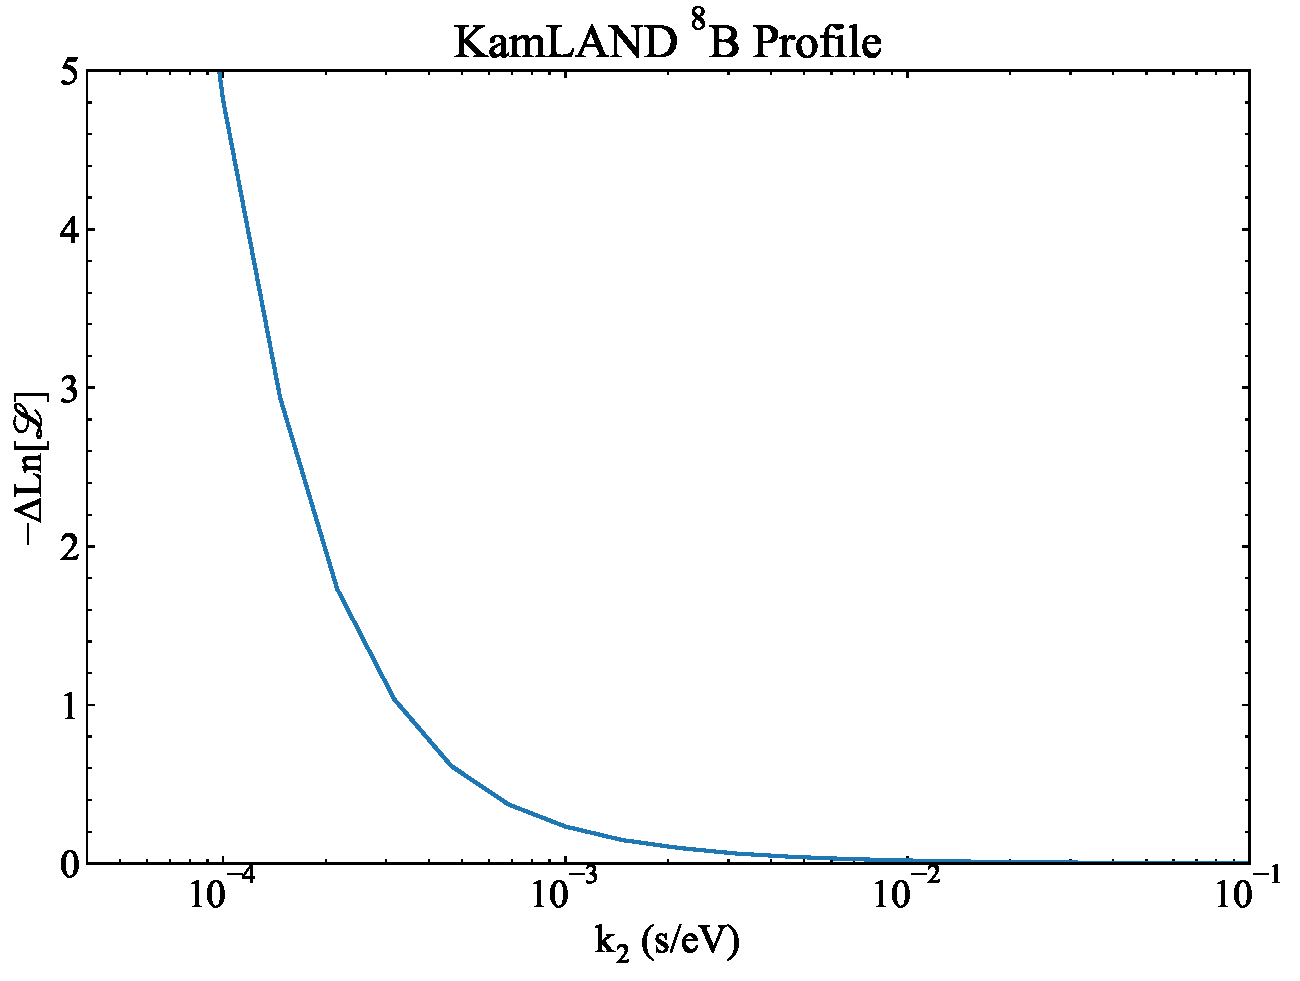
\includegraphics[width=0.5\columnwidth]{kamland_8b}
\caption{The profiled likelihood for the parameter $k_2$ using $^8$B measurements from SuperK~\cite{superkiv}, Borexino~\cite{borexino8b}, and KamLAND~\cite{kamland8b}.}
\label{fig:8b_profiles}
\end{figure}

\subsection{\texorpdfstring{$^7$Be}{Beryllium-7} Constraints}

Borexino~\cite{borexino7be} and KamLAND~\cite{kamland7be} measured the 862~keV line of $^7$Be neutrinos, which account for $90\%$ of the flux from this isotope. 
The average survival probability weighted by the $^7$Be production regions for 862~keV neutrinos is computed for any particular set of neutrino parameters.
Using these survival probabilities, the measured $\Phi_e$ of each experiment is converted to a true $^7$Be flux with \Cref{flux_conv} and compared to the SSM prediction with \Cref{combolike}. 
As these neutrinos are much lower energy, they contain a significant fraction of mass state one. 
Here the lifetime of mass state one, $k_1$, is treated as a nuisance parameter and floated in the fit. 
The profiles in \Cref{fig:7be_profiles} are generated by scanning $k_2$ while floating neutrino parameters and $k_1$.

Note that these constraints are stronger than $^8$B constraints because these neutrinos are lower energy, so measured fluxes near the SSM prediction - even with less precision - can rule out shorter lifetimes.
This holds true (to some extent) for the radiochemical gallium and chlorine experiments discussed in the following sections.

\begin{figure}
\centering
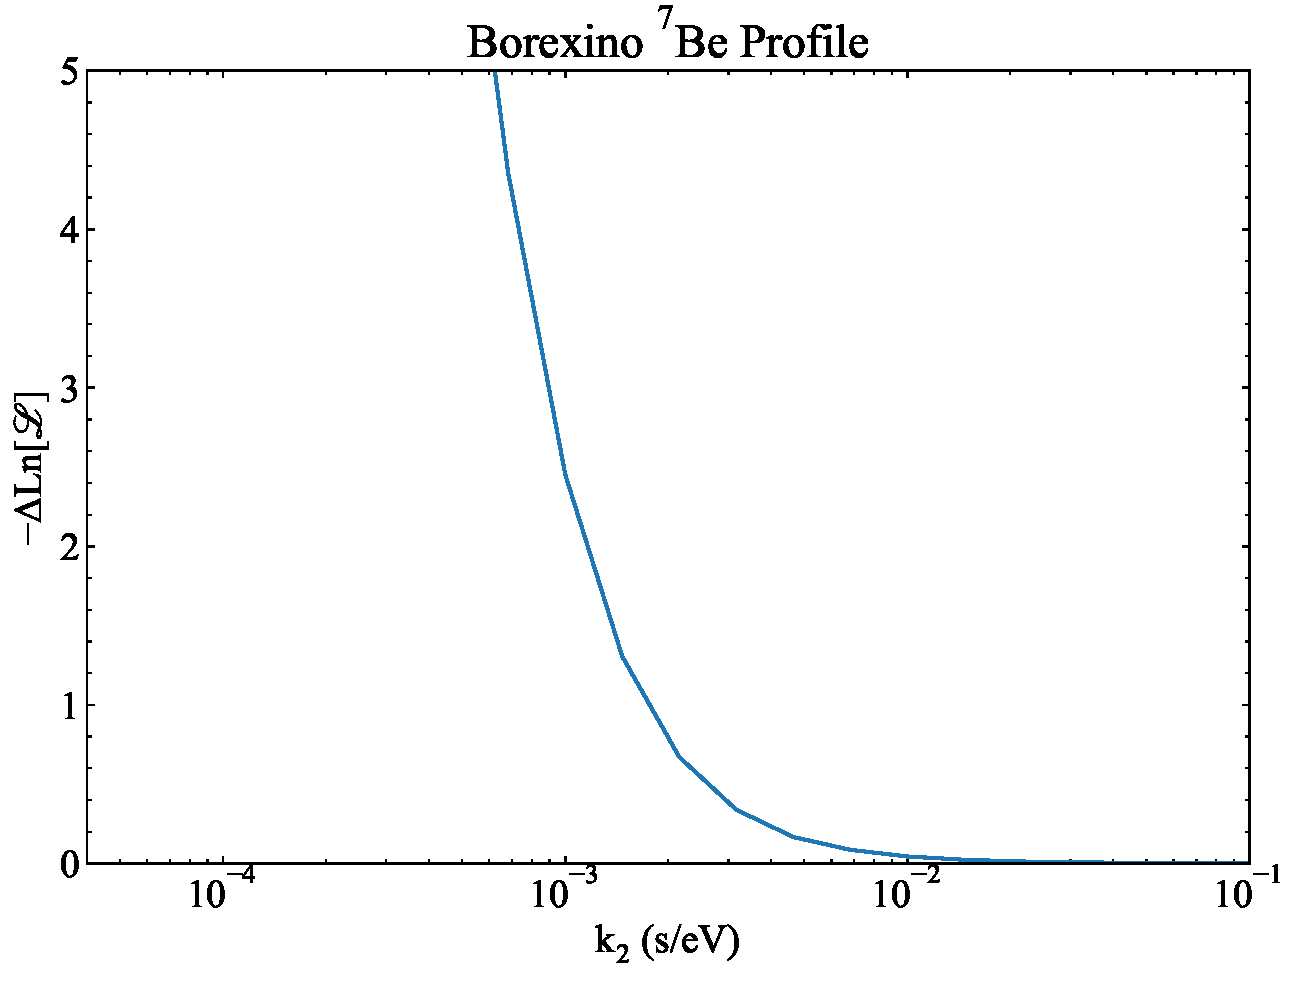
\includegraphics[width=0.58\columnwidth]{borexino_7be}
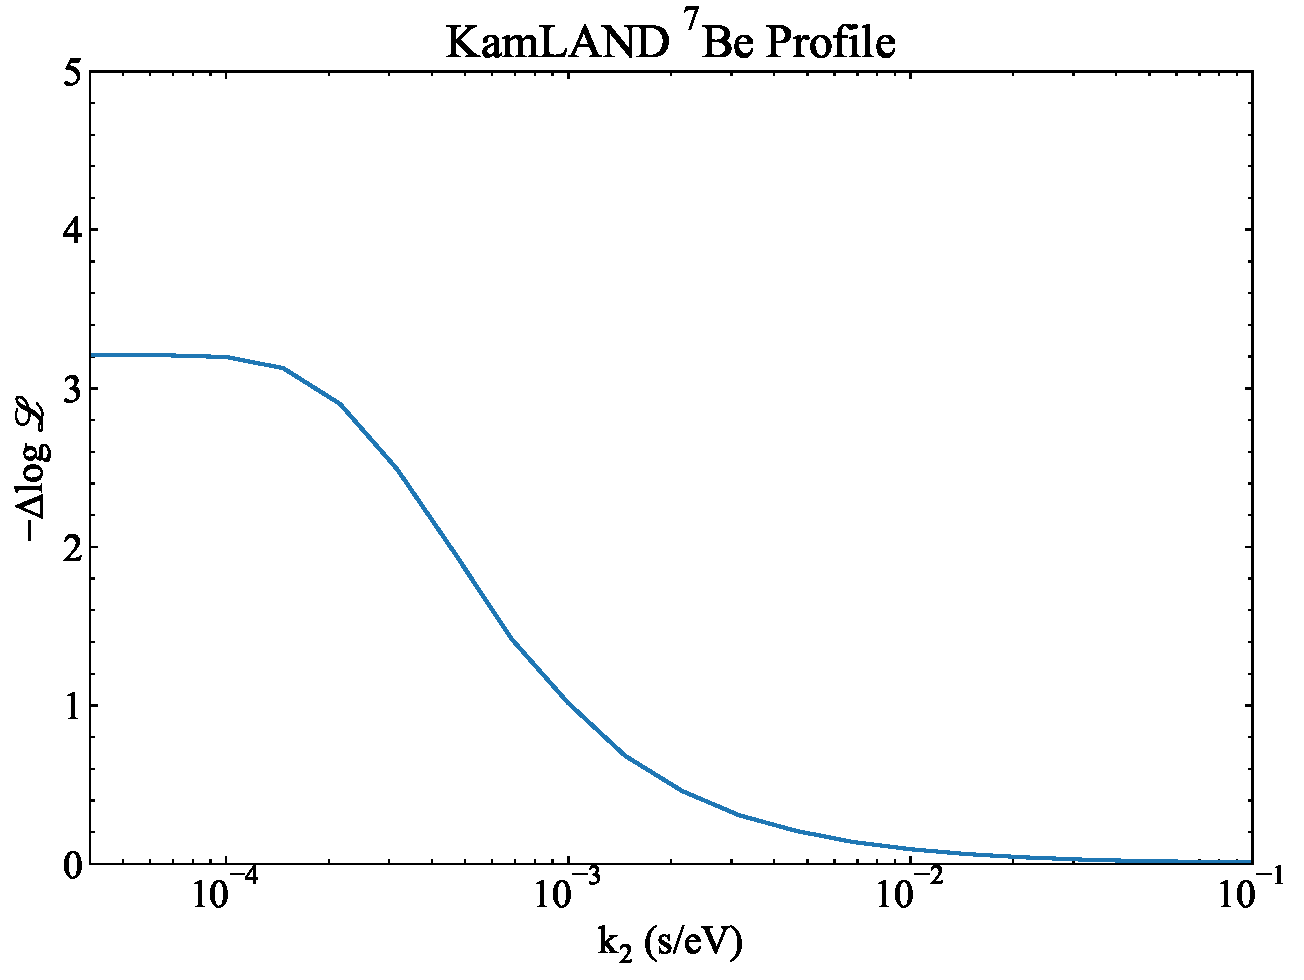
\includegraphics[width=0.58\columnwidth]{kamland_7be}
\caption{The profiled likelihood for the parameter $k_2$ using the $^7$Be 862~keV line measurements from Borexino~\cite{borexino7be} and KamLAND~\cite{kamland7be}. Note the shape of the Borexino profile is quite similar to KamLAND, however, the Borexino measurement excludes short lifetimes at higher significance due to being a more precise measurement.}
\label{fig:7be_profiles}
\end{figure}

\subsection{Gallium Constraints}

The SAGE~\cite{sagecombo} experiment has conveniently combined all gallium solar neutrino measurements into a single value: a rate of solar neutrino interactions on an atom of gallium. 
This requires a bit more effort than the $^8$B and $^7$Be measurements as this rate combines every type of solar neutrino flux, and is related to the fluxes by the gallium neutrino capture cross section.
It is most convenient to compute the expected interaction rate for a particular set of neutrino flux values and mixing parameters and compare this to the measured total rate. 
This follows the analysis described in Section V in~\cite{sagecombo} with the notable exception that the survival probability used here includes neutrino decay.

For each type (that is, originating isotope) of solar neutrino, the average gallium cross section weighted by the energy spectrum and survival probability is calculated for a particular set of neutrino parameters using the appropriate production regions in the Sun for that type.
The gallium cross section used here is the same modified form used in the SAGE analysis~\cite{sagecombo}.
The sum of these average cross sections multiplied by the flux of each type yields the total interaction rate expected on gallium.
This quantity can be directly compared to the measured rate with a likelihood term similar to \Cref{combolike}.

A profiled likelihood is arrived at in a similar way as described above: neutrino parameters, SSM fluxes, and lifetime of mass state one are floated while $k_2$ is scanned. 
Neutrino parameters and SSM fluxes are constrained with the same priors as elsewhere in this analysis.
The result is shown in \Cref{fig:ga_profiles}.

\begin{figure}
\centering
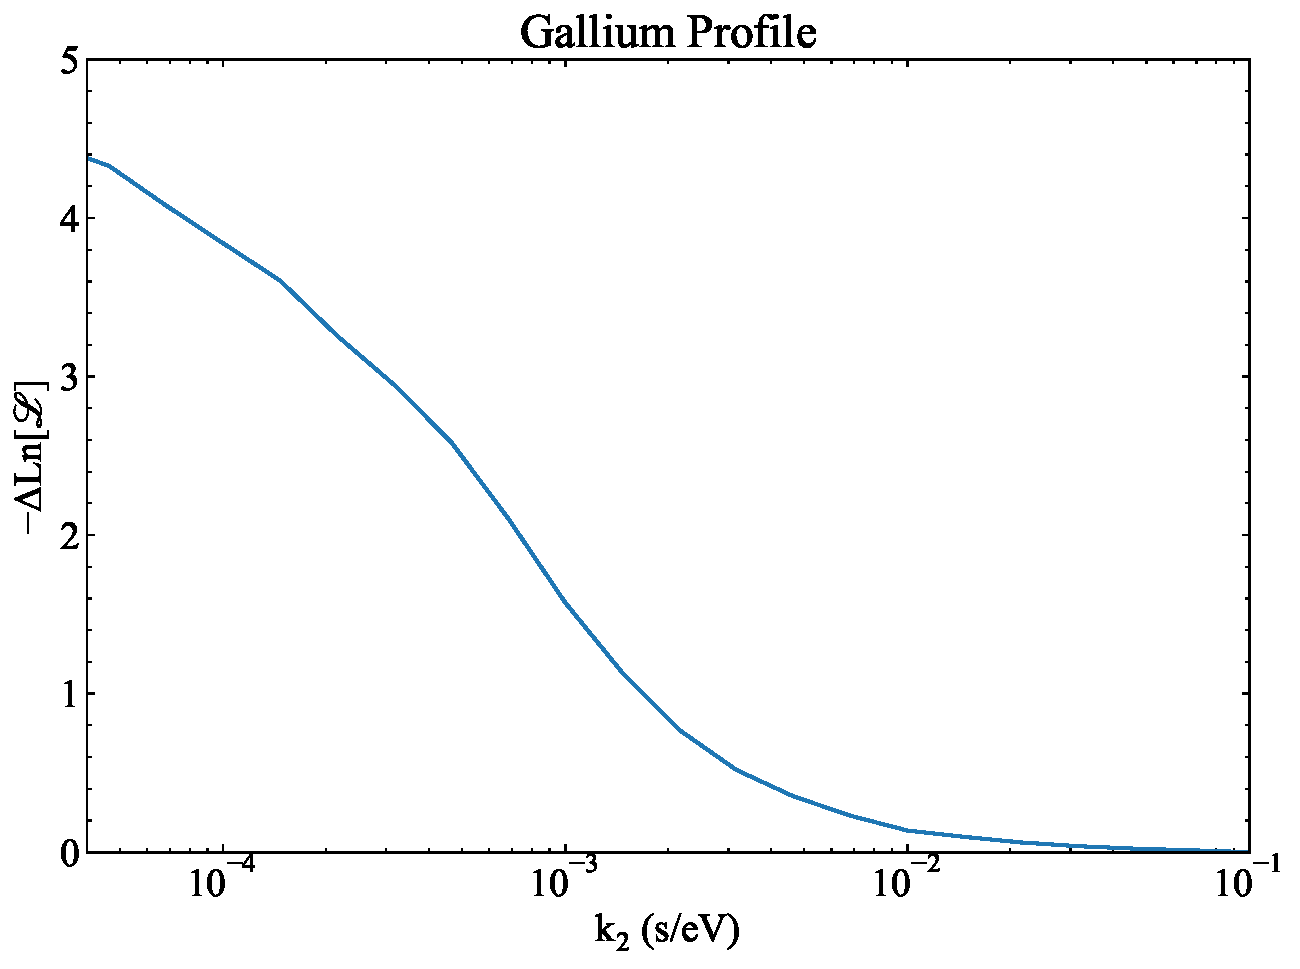
\includegraphics[width=0.58\columnwidth]{gallium_8b}
\caption{The profiled likelihood for the parameter $k_2$ using the combined measurement of all gallium experiments~\cite{sagecombo}.}
\label{fig:ga_profiles}
\end{figure}

\subsubsection{Validation}

As this is more complicated than a simple constraint, some additional verification is needed to ensure there are no issues with the code.
To that end I have reproduced the per-component interaction rate from Table IV of~\cite{sagecombo} in \Cref{tbl:gallium} using the mixing parameters and approximate form of the survival probability from that same reference.
As these values are nearly identical to those reported in the original publication, my calculation of cross sections and total rates appears consistent.

Note that~\cite{sagecombo} uses an approximate form of the survival probability whereas for all other parts of this analysis I have numerically diagonalized the MSW Hamiltonian (see \Cref{lifetime_model}).
A notable difference between these two approaches is that the approximate forms assume a uniform solar density for each flux, while my numerical method accounts for the density profile in the regions where these neutrinos originate.
Using my numerical computation instead of the approximate form yields slightly different numbers (also shown in \Cref{tbl:gallium}). 
Both total rates are consistent with the Gallium measurements $66.1\pm3.1$~SNU~\cite{sagecombo} at one sigma, and the numerical method is used for other parts of this analysis.

With the calculation of the expected rate validated, the remaining step of including gallium results in this analysis is a comparison to the measured rate with a term like \Cref{combolike}.

\begin{table}
\centering
\begin{tabular}{c|r|r|r}
Component &~\cite{sagecombo} Rate (SNU) & Approximate $P_{ee}$ (SNU) & Numerical $P_{ee}$ (SNU) \\ \hline
$pp$		& 39.35	&	39.34 	&	39.18	\\
$pep$		& 1.43 	&	1.43 	&	1.35 	\\ 
$^7$Be		& 18.73	&	18.74	& 	18.78	\\
$^{13}$N	& 0.89 	&	0.89	&	0.85	\\ 
$^{15}$O	& 1.23 	&	1.23	&	1.13	\\ 
$^{17}$F	& 0.03 	&	0.03	&	0.03	\\
$^8$B		& 4.64 	&	4.63	&	4.54	\\ 
$hep$		& 0.02 	&	0.02	&	0.02	\\ \hline
Total		& 66.31	&	66.32 	&	65.80	\\ \hline
\end{tabular}
\caption{\label{tbl:gallium}Shown here are the predicted interaction rates of each neutrino flux with Gallium computed with the code developed for this analysis using both the approximate survival probability forms in~\cite{sagecombo} and the numerical forms used elsewhere in this analysis. Results from~\cite{sagecombo} are reproduced for reference.}
\end{table}

\subsection{Chlorine Constraints}

The analysis of radiochemical measurements of interactions on chlorine is very similar to that of the gallium experiments described above. 
So, a similar analysis as done for gallium was performed here, but using the measured rate from the Homestake~\cite{homestake} experiment, $2.56\pm0.23$~SNU on $^{37}$Cl, along with the chlorine cross sections used for that analysis.
The result of the profile are found in in \Cref{fig:cl_profiles}.

\begin{figure}
\centering
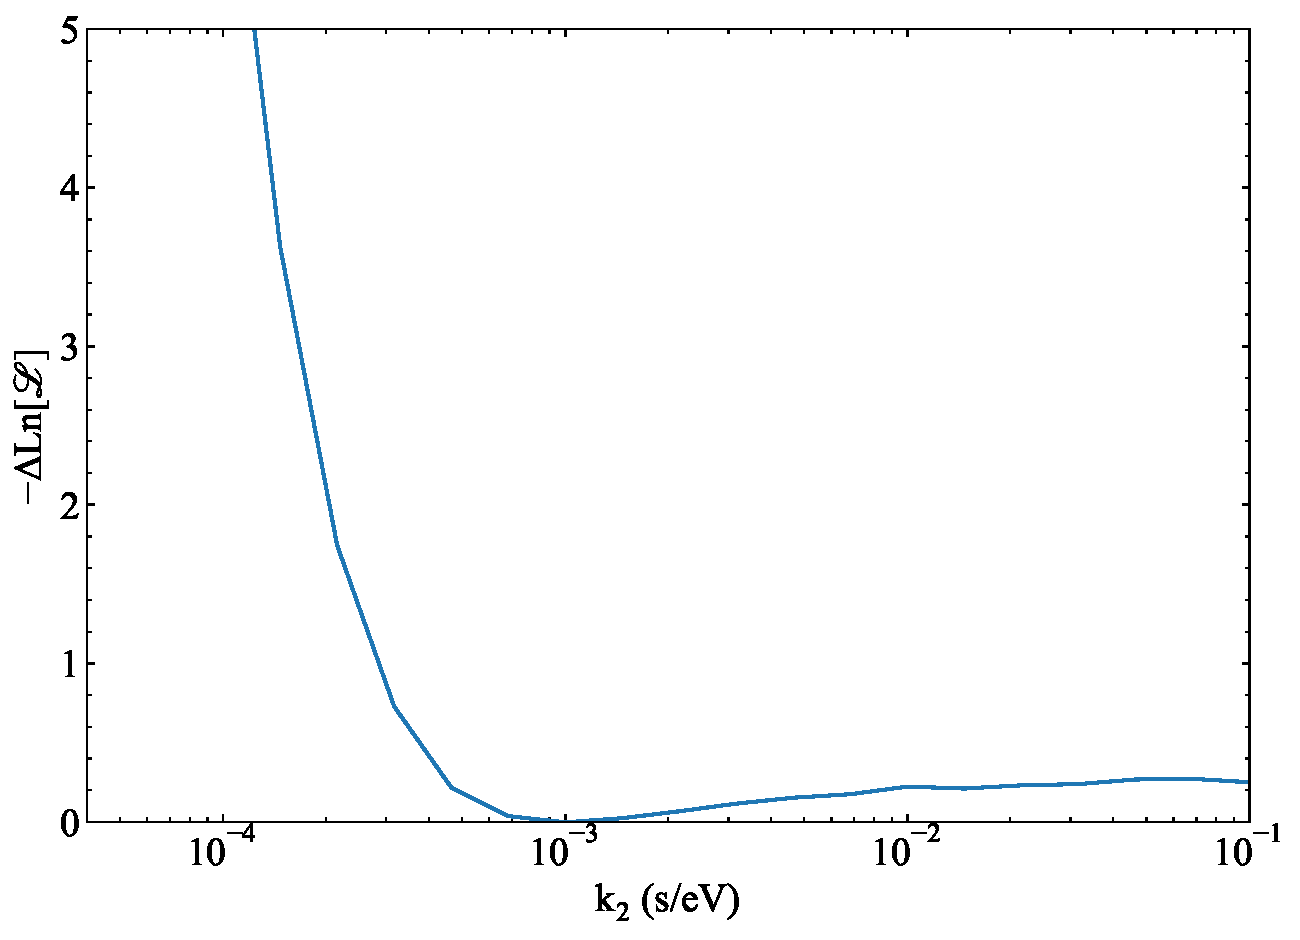
\includegraphics[width=0.58\columnwidth]{chlorine_8b}
\caption{The profiled likelihood for the parameter $k_2$ using the measurements from Homestake~\cite{homestake}.}
\label{fig:cl_profiles}
\end{figure}


\subsubsection{Validation}
The Homestake~\cite{homestake} experiment does not go into detail about expected rates from separate components.
Also, the references cited there tend to assume $P_{ee} = 1$ when calculating expected rates, which is not a useful comparison to make with this analysis.
A more recent paper~\cite{bachall_lma} does a modern calculation of the expected interaction rates per flux component that is directly comparable to the model used here.

Using the fluxes and mixing parameters quoted in Table I of~\cite{bachall_lma}, I have reproduced the interaction rates central values for Chlorine in \Cref{tbl:chlorine} and compared to the large mixing angle (LMA) solution from Table I of~\cite{bachall_lma}.
The column showing the `old' parameters are using the fluxes and mixing parameters from~\cite{bachall_lma} while the column showing `new' parameters uses the SSM and mixing parameters used elsewhere in this analysis.
In all cases there is pretty good agreement with the measured rate from Homestake and between models.

\begin{table}
\centering
\begin{tabular}{c|r|r|r}
Component &~\cite{bachall_lma} Rate (SNU) & `Old' Parameters (SNU) & `New' parameters (SNU) \\ \hline
$pp$		& 0.0	&	0.00 & 0.00		\\
$pep$		& 0.1 	&	0.13 & 0.12		\\ 
$^7$Be		& 0.46	&	0.45 & 0.30		\\
$^{13}$N	& 0.05 	&	0.05 & 0.02		\\ 
$^{15}$O	& 0.16 	&	0.17 & 0.07		\\ 
$^8$B		& 1.8 	&	1.82 & 2.20		\\ 
$hep$		& 0.1 	&	0.07 & 0.01		\\ \hline
Total		& 2.6	&	2.69 & 2.75		\\ \hline
\end{tabular}
\caption{\label{tbl:chlorine}Shown here are the predicted interaction rates of each neutrino flux with Chlorine both from an independent calculation~\cite{bachall_lma}, using this analysis' code with the `old' mixing and flux parameters in that reference, and again with the flux and mixing parameters used elsewhere in this analysis.}
\end{table}

\subsection{Combined Result}
\label{sec:combobreaker}

The likelihood profiles of individual experiments are multiplied (negative log likelihoods added) together to arrive at a combined likelihood profile shown in \Cref{fig:combined_profile}. 
Explicitly this includes: $^8$B measurements from KamLAND, Borexino, Super-Kamiokande (I,II,III,IV) and this analysis of SNO data, $^7$Be measurements from KamLAND and Borexino, and total rate measurements from all gallium experiments (SAGE+GNO+GALLEX) plus the Homestake results on chlorine. 
The $99\%$ C.L. lower bound for the lifetime of mass state two is $>10.41\times10^{-4}$~s/eV. 
This is better than the previous analysis for a few reasons: KamLAND results were not previously included, and both Borexino and Super-K published updated analyses compared to the data used in the previous limit. 
Notably the presence of a relatively significant minimum in the new SNO results is not particularly beneficial here since it occurs near the location of the limit.

\subsection{Cross-Check with Previous Limit}

The analysis that set the best limit~\cite{picoreti} did not go into detail as to how their analysis was performed, or which SSM values were used as a reference.
This makes it difficult to precisely reproduce their results, however, since they do list the experimental results used, I can repeat my analysis using those experimental results and see if I get a similar limit.

The experiments used in the previous best limit were: Homestake (Cl), Sage (Ga), GNO+GALLEX (Ga), Borexino's first $^7$Be publication, SNO's 3-phase analysis, and Super-K (I). 
Homestake and the gallium experiments have not been updated and are handled as described above.
Borexino and Super-K (I) are handled as described above but with the less-precise flux determinations of those two analyses. 
The SNO 3-phase results are handled in an analogous way to Super-K results using only the flux information.


In \Cref{fig:cross_check_profile} I have combined the profiles from these measurements and arrived at a limit of $>7.58\times10^{-4}$~s/eV at $99\%$ C.L., a bit better than~\cite{picoreti}'s quoted $>7.2\times10^{-4}$~s/eV at $99\%$ C.L..
That this is quite close to the limit set by~\cite{picoreti} indicates that these two analyses are consistent even if the methods presumably differ.
Unfortunately with the brevity of the previous paper a more direct comparison does not seem possible.

\begin{figure}
\centering
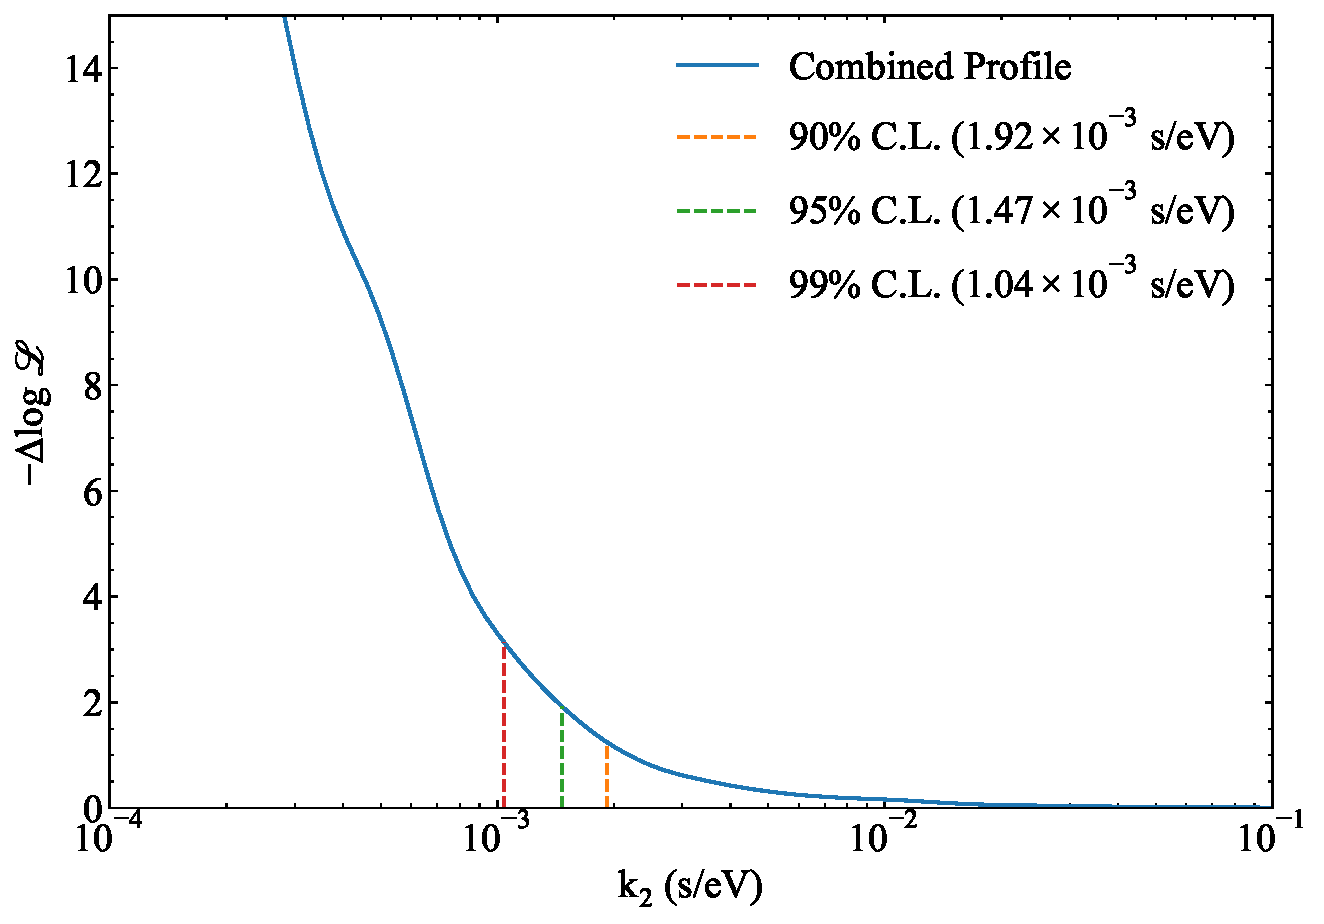
\includegraphics[width=0.85\columnwidth]{combined_profile}
\caption{The combined profiled likelihood described in \Cref{sec:combobreaker}.}
\label{fig:combined_profile}
\end{figure}

\begin{figure}
\centering
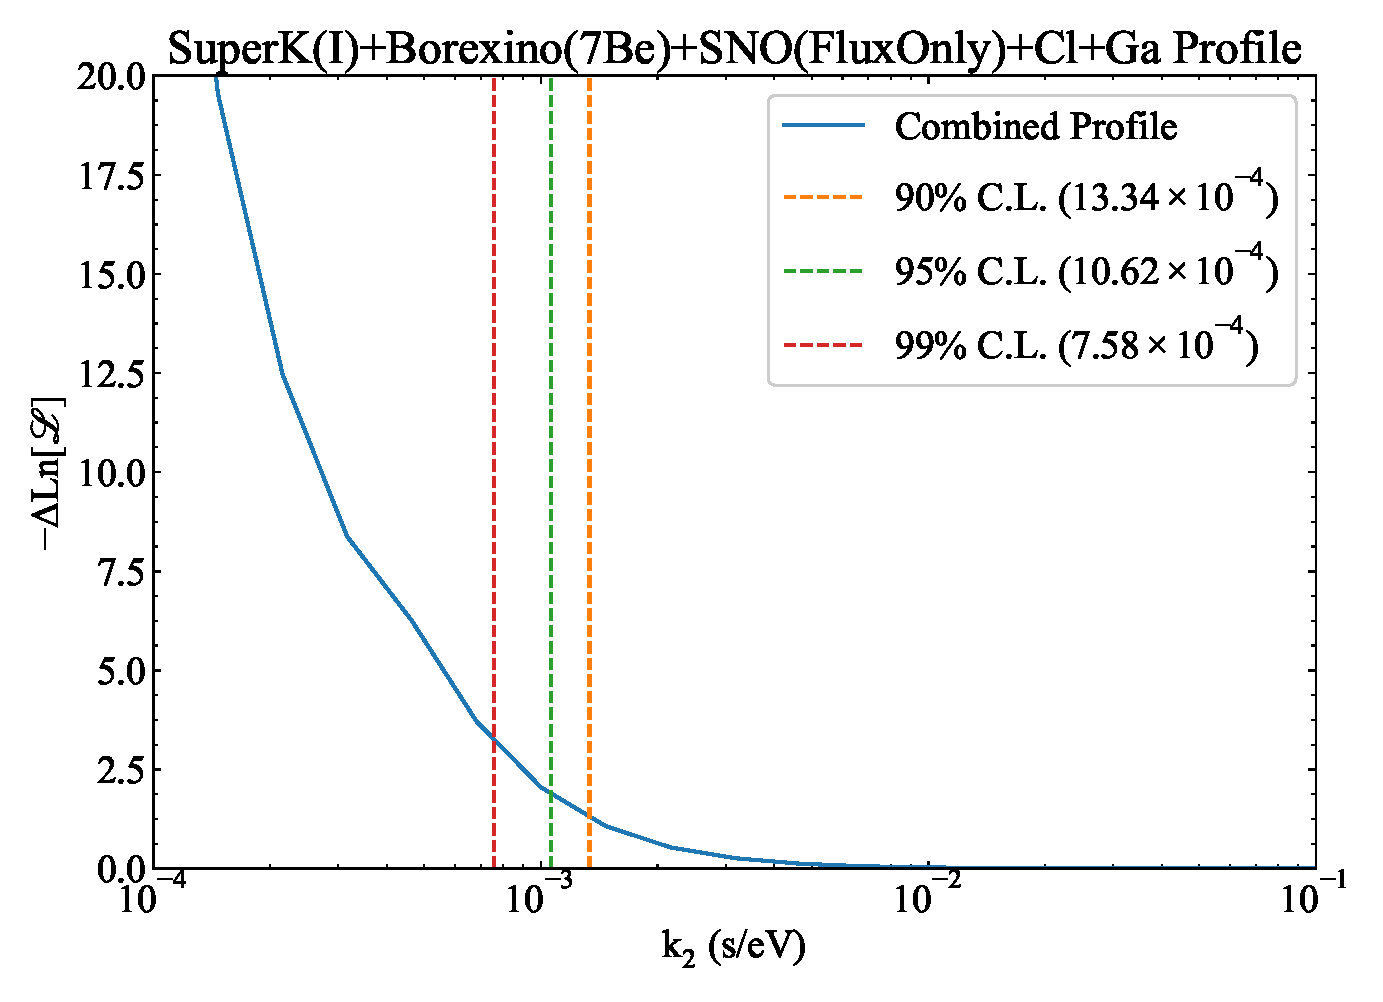
\includegraphics[width=0.85\columnwidth]{cross_check_profile}
\caption{The combined profile intended to reproduce the result in~\cite{picoreti} by using the same experimental measurements. Notably the analysis methods are not identical so the results should be similar but do not match exactly.}
\label{fig:cross_check_profile}
\end{figure}

\renewcommand{\bf}{\bfseries}

\chapter{Cherenkov Optical Calibration Source for SNO+}
\label{ch:chsrc}

SNO+ has over 9500 Photo-Multiplier Tubes (PMTs), which detect photons produced inside the target (water or liquid scintillator).
Within the SNO+ calibration plan~\cite{gann:2013} it is vital to extract and monitor the overall light collection efficiency of these PMTs, because this determines the energy response of the detector.
The Cherenkov source was designed to produce a well understood optical signal, which can be used to measure these quantities.

The Cherenkov source is able to make the measurements in a way nominally independent of the target as described in \Cref{chap:motivation}. 
The detailed design of the source is discussed in \Cref{chap:design}. 
The construction procedures are briefly covered in \Cref{chap:construction}.
Tests  \Cref{chap:tests}.
Finally \Cref{chap:water_phase} discusses the deployment of this source in SNO+ water phase and an analysis of the data taken during the deployment.

\section{Motivation}
\label{chap:motivation}

For both Chernekov and scintillation light, visible energy is proportional to the total number of generated photons.
In the case of a water target, the production of Cherenkov light is well understood and can be accurately simulated from first principles.
In order to calibrate the energy response of the detector, a radioactive source with a well understood energy spectrum, such as an \N source, can be deployed and used to calibrate a simulation model.
In this case, with Cherenkov production being simulated accurately, only the response of the detector needs to be tuned in simulation to reproduce the data.

When SNO+ switches to liquid scintillator, this situation is more complicated because the scintillation process is not as easy to model.
For instance, the photon yield typically must be measured for any independent batch of scintillating liquid, whereas the production of Cherenkov light is calculable. 
This means that calibrating the energy scale of the detector with something like an \N source would be unable to disentangle changes to scintillation output from changes in detector response.
Disentangling these two effects can be achieved by deploying a source that produces a well understood and easily simulated optical signal. 
The Cherenkov source is designed to produce such a signal through tagged Cherenkov events.


\section{Source Design}
\label{chap:design}

The Cherenkov light produced by this source will come from stopping beta decay electrons from \Li in UV-absorbent (UVA) acrylic, and is based on the SNO \Li source design and experience~\cite{Tagg:2002,Tagg:2001}.
The choice of UVA acrylic was made to block the UV component of Cherenkov light, which would be absorbed and reemitted by the scintillator.
Thus, the remaining light that propagates through the SNO+ detector is quasi-independent of the optical properties of the LAB-PPO scintillator. 
This visible Cherenkov light is easy to model, allowing for a measurement of detector response nominally independent of the target material.

\begin{figure}[]
\center{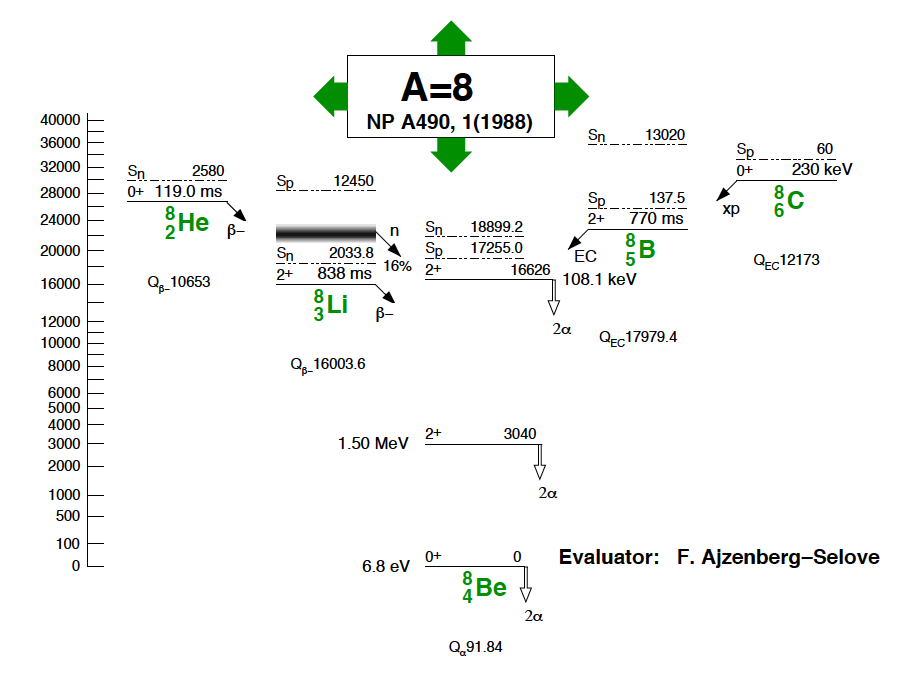
\includegraphics[width=.7\textwidth]{Ais8DecayScheme.png}}
\caption{\label{fig:decayscheme} A=8 decay scheme. Taken from~\cite{Tagg:2001}.}
\end{figure}

The decays following \Li in the decay chain (see \Cref{fig:decayscheme}) results in a very fast alpha decay following the production of the beta.
The chamber in which the decay occurs will be filled with helium gas in which these alphas will produce scintillation light.
This scintillation light is hard UV, around 80-nm, and impossible for traditional PMTs to detect, so the chamber will contain a wavelength shifter,  Tetraphenyl Butadiene (TPB), to convert the UV photons to approximately 420-nm light.
These shifted photons can then be detected by an internal PMT to produce a tag signal for the primary \Li decays.

Because this is a calibrated light source, any other processes that may produce optical photons should be well understood and, where possible, eliminated with design choices.
The alpha scintillation, especially including the wavelength shifted photons, must be contained within the source. 
Additionally, any energetic particles produced in the \Li decay must be taken into account.
The UVA acrylic is designed thick enough to stop all of the \Li betas from exiting, however, these energetic electrons can produce Bremsstrahlung gammas that do escape the source.
When deployed in water phase these gammas will not produce sufficient light to interfere with analysis of the data, however, in scintillator phase these will be a significant background to the measurement, and must be cut in an offline analysis. 

\subsection{Cherenkov Event Generation}

The \Li (t$_{1/2}$=0.838\,s) isotope is created using a deuterium-tritium neutron generator in conjunction with a $^{11}$B target.
Neutron captures on $^{11}$B produce $^{12}$B, which alpha decays to \Li.
The \Li is transported by helium gas to the spherical decay chamber at the center of the source as shown in Figure~\ref{fig:design-1}. 
The energetic beta particles produced by the decay are stopped in the 6\,cm-thick spherical acrylic wall and produce Cherenkov light. 
The alphas from the subsequent $^{8}$Be decay produce scintillation light in the helium, which is then wavelength shifted by TPB present in the lining of the decay chamber.
A small PMT in the neck of the source detects this scintillation light, generating a tagging signal for the event. 

\subsection{Source Geometry}
The Cherenkov source consists of three main parts: the acrylic decay chamber, the PMT assembly inside the neck, and the steel housing inherited from the SNO \Li source. See Figures~\ref{fig:design-1} and~\ref{fig:design-2}.
See~\cite{wallig:2015} for the complete set of technical drawings for the Cherenkov source. 3D-rendered drawings are used in this section to identify the different parts of the source.

\begin{figure}
\center{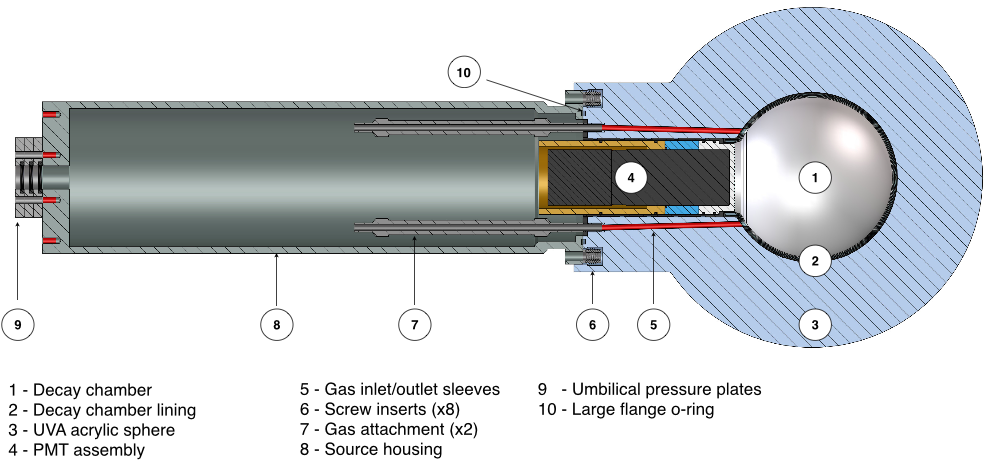
\includegraphics[width=1.0\textwidth]
{Design-1.png}}
\caption{\label{fig:design-1}Schematic of the fully assembled Cherenkov source.}
\end{figure}

\begin{figure}
\center{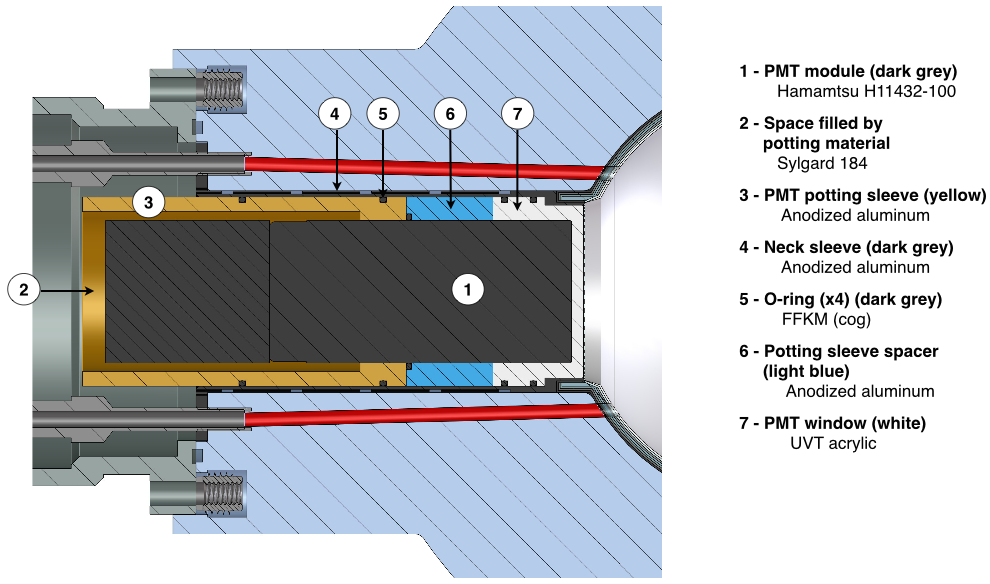
\includegraphics[width=1.0\textwidth]
{Design-2.png}}
\caption{\label{fig:design-2}Detail of the PMT assembly.}
\end{figure}

\subsubsection{Decay chamber}

The decay chamber is roughly a sphere made out of UVA acrylic supplied by RPT (Reynolds Polymer Technology). 
This is machined in two halves, which must be bonded using Weld-on\,\#40. Details on this procedure are found in \Cref{sec:bond}.
The inside of the decay chamber is lined with an opaque, reflective and wavelength-shifting coating, which consists of 4 layers of paint, which are discussed further in \Cref{sec:lining}.
A thin neck-sleeve made from anodized aluminum is potted in place using Sylgard 184 to accept the tag PMT assembly. 
It serves to ensure light-tightness, specifically around the PMT window.
Two thin steel capillaries are potted inside the gas inlet and outlets holes with Sylgard~184. These are needed in order to ensure light-tightness and do not form gas seals. The inlet lines are threaded into the acrylic and the threads are potted in with Sylgard~184. 
The attachement of the decay chamber to the steel housing is done by way of 8 stainless steel screws. 8 screw-inserts are glued in place inside the top of the decay chamber using Weld-on\,\#40.
A single large o-ring is placed in the plane where the steel housing is connected to the decay chamber. 
This seal prevents target material ingress into the source body, while the decay chamber is further isolated by a second set of o-ring seals.

\subsubsection{PMT assembly}

The PMT module fits inside the neck to observe the scintillation light inside the decay chamber. 
The module is a Hamamatsu H11432-100, which has an integrated high voltage supply that requires only low voltage (+5V) to operate. 
This module is potted into an anodized aluminum holder (\cite{wallig:2015}, page 8) using a silicone encapsulate Sylgard~184. 
On the front of this PMT module is a UVT acrylic window that faces into the decay chamber. This is intended to contain the helium gas while allowing the wavelength shifted tag signal photons to reach the tag PMT.
There are 4 small o-rings between the PMT assembly and the neck-sleeve, they are made from FFKM material.

\subsubsection{Steel housing}
The housing (\cite{wallig:2015}, page 12) and the gas connections (\cite{wallig:2015}, page 13) are inherited from the SNO \Li source. 
The housing is made of stainless steel and can be shortened if needed. 
To handle the different types of connections used in different phases of SNO+, a flange was added to the original steel housing, as shown in Figure~\ref{fig:flange}. 
The gas connections can also be changed if needed by modifying the gas lines threaded into the decay chamber.
The steel housing is electropolished and cleaned to remove any surface contaminates before the final assembly and deployment of the source.

\begin{figure}
\center{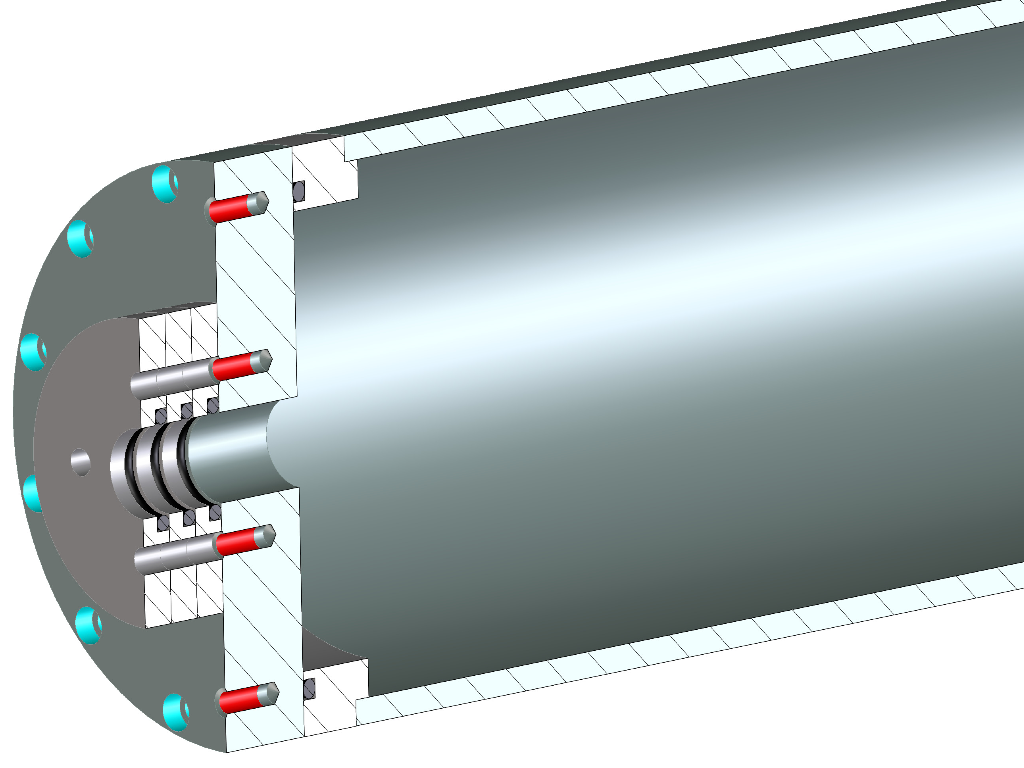
\includegraphics[width=.5\textwidth]
{flange.png}}
\caption{\label{fig:flange} Schematic of a suggested flange to be welded at the top of the source housing. }
\end{figure}

\subsection{Deployment hardware}

For deployment during the SNO+ water-phase, the SNO \Li umbilical to transport \Li into the source was re-used.
Figure~\ref{fig:sno_umbilical} shows the cross-section of this umbilical. It contains the required gas-transport lines in addition to the electrical wires; one for the PMT signal and three for the low-voltage for the PMT (ground, power, control voltage). 
The umbilical currently has no connector. 
Just as was done for SNO, the plan is to connect the gas hoses and wiring for the PMT by hand while the top of the source (steel housing) is exposed. 
Then the sealing pressure plates (Figure~\ref{fig:pressureplates}) are slid down and bolted together. 
The so-called 'lighthouse' attachment, see Figure~\ref{fig:connection}, sits on the endcap and is used to attach the source to SNO+'s source deployment hardware.

\begin{figure}
\begin{subfigure}{.57\textwidth}
\center{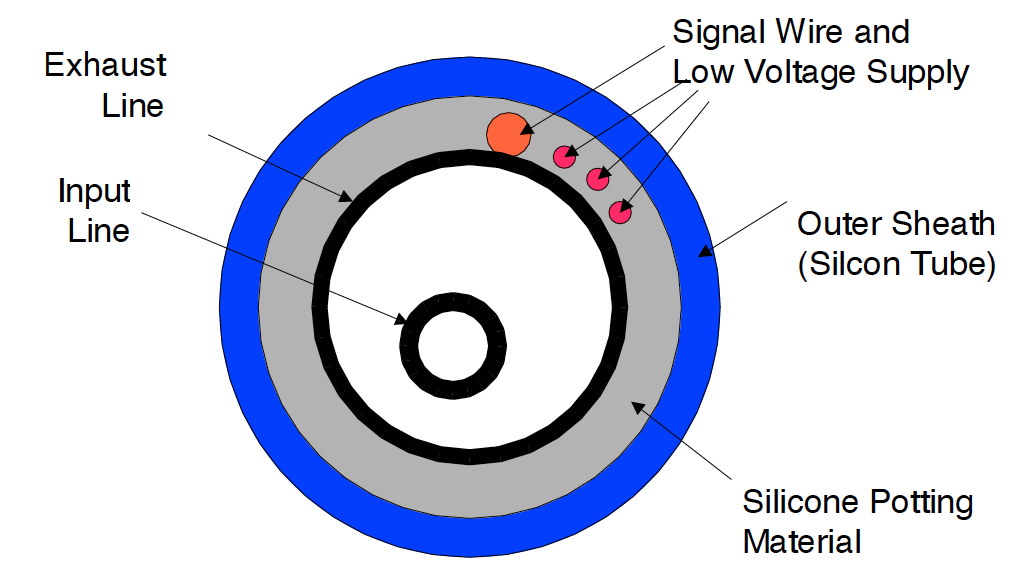
\includegraphics[width=1.0\textwidth]
{8Li-Umbilical.png}}
\caption{\label{fig:sno_umbilical} The SNO \Li umbilical cross-section. Taken from~\cite{Tagg:2001}.}
\end{subfigure}
\hspace{0.5cm}
\begin{subfigure}{.35\textwidth}
  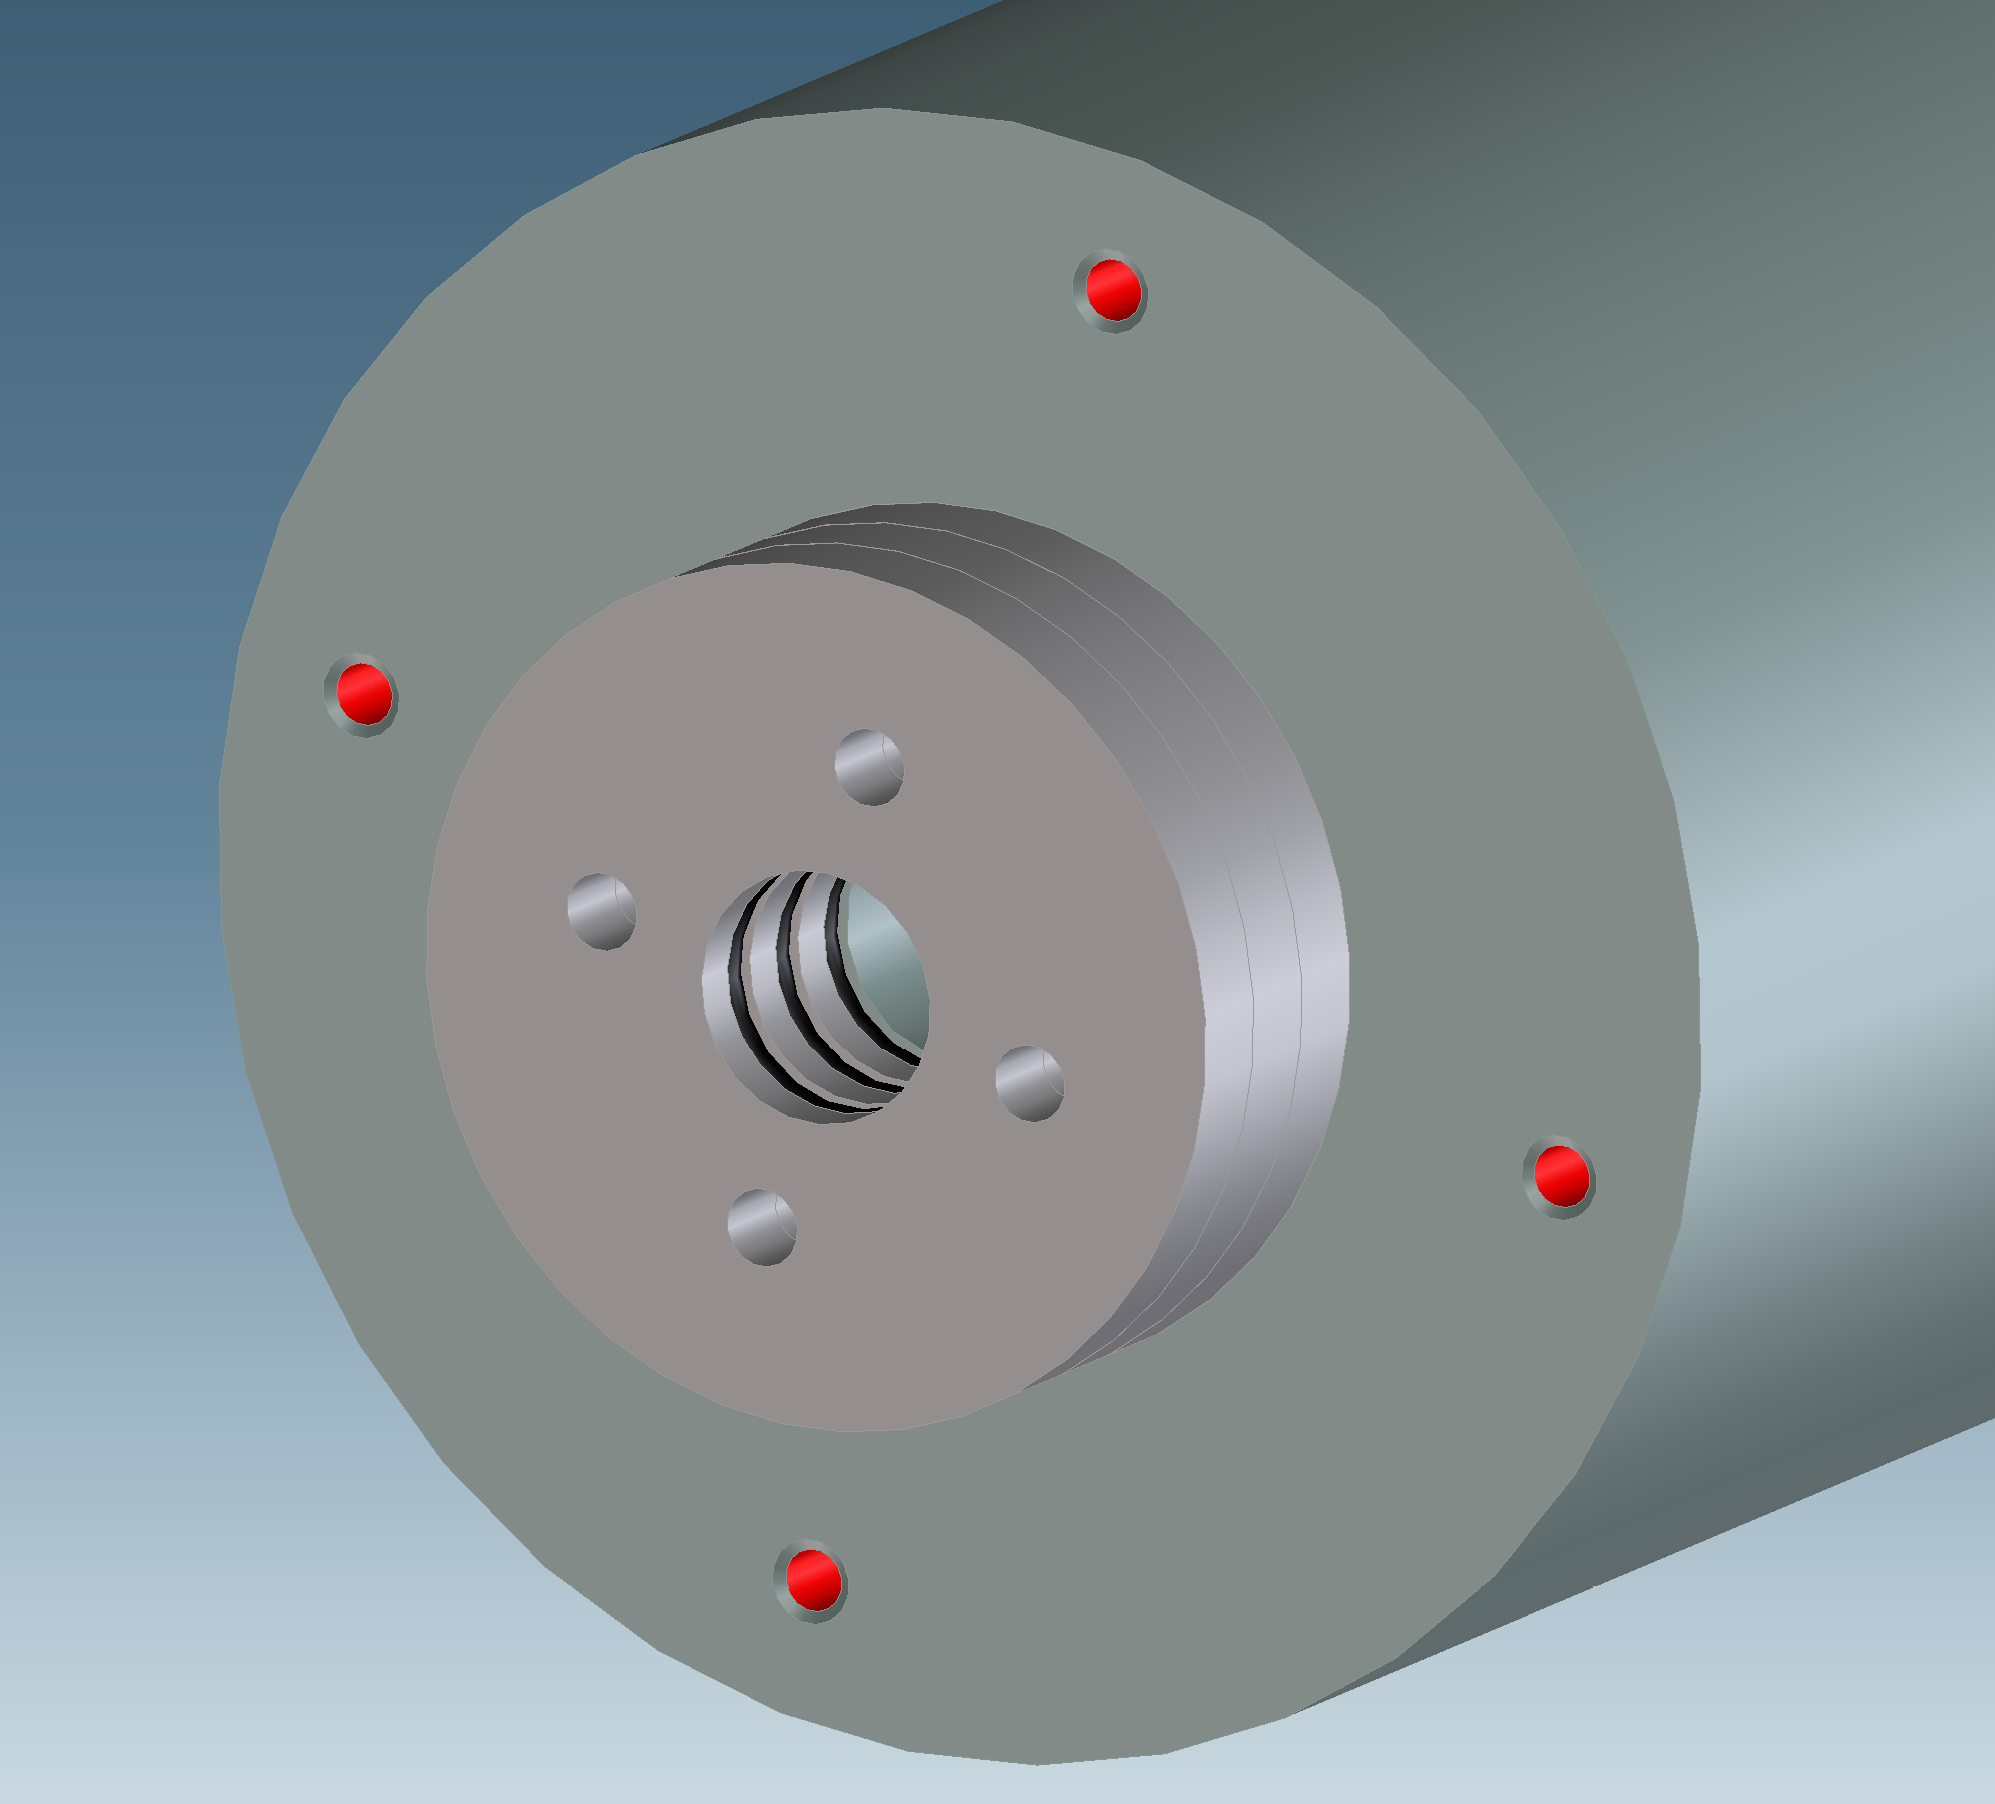
\includegraphics[width=\textwidth]{HousingTop.png}
  \caption{\label{fig:pressureplates} The sealing pressure plates.}
\end{subfigure}
\caption{Details of the umbilical and the water-phase umbilical connection to the source housing.}
\end{figure}

\begin{figure}
\center{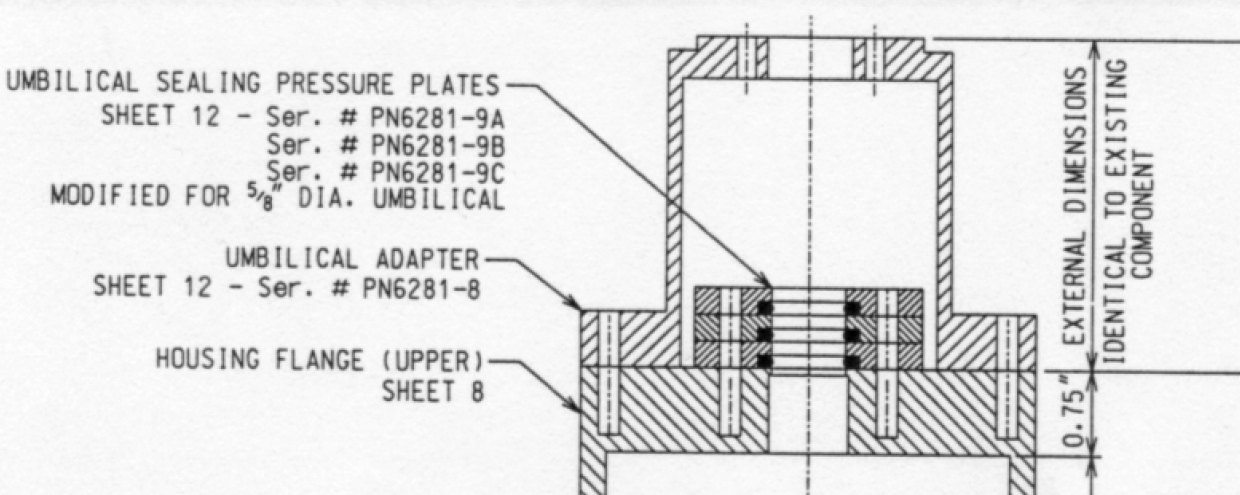
\includegraphics[width=.8\textwidth]
{UmbilicalConnection.png}}
\caption{\label{fig:connection}Detail of the SNO \Li technical drawing, showing the top assembly with the pressure plates and the 'lighthouse'. Taken from~\cite{Tagg:2001}.}
\end{figure}

The umbilical that will be used for deployment in the liquid scintillator still needs to be produced. 
It is expected to be of a similar design as the SNO \Li umbilical with the difference that there will be a source connector permanently attached to the umbilical. 
An adapter then needs to be designed to connect to the Cherenkov source. 

\section{Decay Chamber Construction}
\label{chap:construction}

The Cherenkov source decay chamber is a hollow acrylic sphere.
It is formed out of two acrylic slabs that are bonded together.
The annealing, bonding, decay chamber lining and PMT potting are described in the next sections.
The bonding, painting and storage of the decay chamber was done inside a class-1000 clean room at LBNL.
The construction of the Cherenkov source decay chamber has roughly the following steps:

\begin{enumerate}
    \item Pre-anneal: the acrylic is pre-annealed at the production site (RPT).
    \item Machine cycle 1 (see~\cite{wallig:2015}, page 2): hollow out the decay chamber and neck from the two slabs. Machine holes for alignment pins. 
    \item Polish: the inside of the decay chamber is polished using NOVUS heavy and fine scratch remover (Diatomaceous earth/Silica)~\cite{polish}. 
    \item Sand: the bond-plane is sanded to prepare for the bond using NORTON Blue-Bak waterproof paper (Silicon carbide) grit, 220, 320, 400, 600~\cite{sand}.
    \item Ultra high vacuum cleaning.
    \item Anneal: the two machined slabs are annealed.
    \item Ultra high vacuum cleaning.
    \item Mask: masking paint (Micro Mask MI-7~\cite{masking}) is used to protect the inside of the decay chamber from the cement. This product is easily removed with water.
    \item Bonding: bond the two halves together using Weld-on \#40, an acrylic cement. 
    \item Remove masking: once the cement has set, remove the masking from the inside of the decay chamber.
    \item Machine cycle 2 (see~\cite{wallig:2015}, pages 5 and 6): remove excess acrylic to form sphere, drill the gas inlet/outlet holes, machine o-ring groove.
    \item Ultra high vacuum cleaning.
    \item Decay chamber lining: use paints and TPB to line the inside of the decay chamber. This also requires potting of the neck sleeve and gas inlet and outlet sleeves.
    \item PMT potting: pot the tag PMT inside the PMT sleeve.
    \item Assembly and testing.
\end{enumerate}

\subsection{Acrylic Annealing}

Before bonding, the acrylic blocks must be annealed to remove any residual stresses. The annealing process raises the temperature of the acrylic in a controlled way so that stress frozen into the cold solid acrylic can relax away, and then lowers the temperature in a controlled way so that new stress is not developed. This is necessary to ensure that there are no residual stresses that will cause reduced optical clarity (crazing) or mechanical failure (poor bond). The blocks were placed in an annealing oven shown in Figure~\ref{fig:oven} that was programmed to follow an annealing curve containing an initial ramp, a soak phase, and a cool-down ramp. Most information for acrylic annealing was obtained from an Air Force / Navy acrylic fabrication specification MIL-P-6997B(ASG) and the Handbook of Acrylics. The thickness of the acrylic during annealing is 152~mm, which is used for calculating the lengths of the annealing stages, and a soak temperature of 80\degree C was chosen to ensure the acrylic can relax without risking deformation of the machined surfaces. The final annealing curve is shown in Figure~\ref{fig:annealing}.

\begin{figure}
\begin{subfigure}{.54\textwidth}
  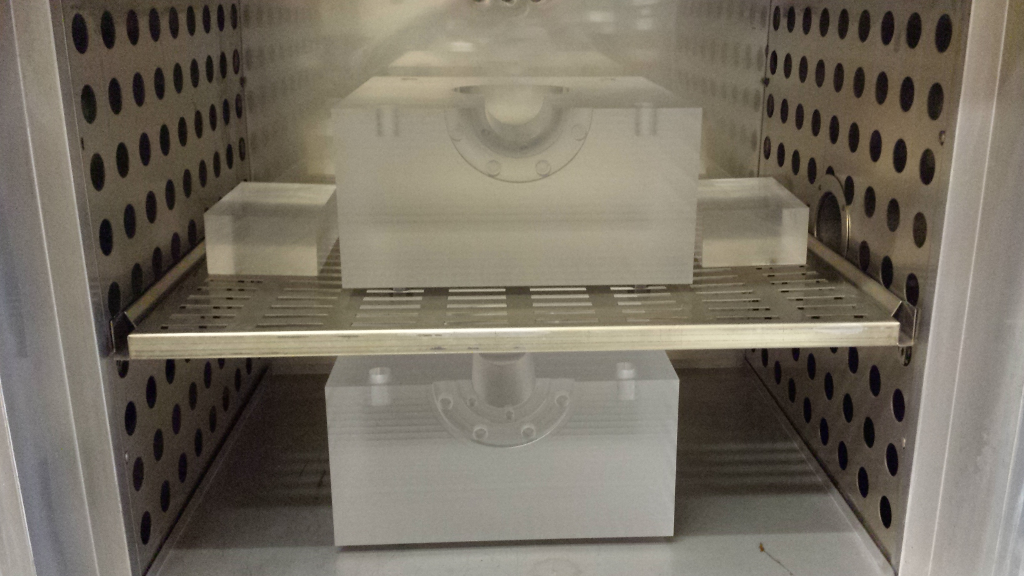
\includegraphics[width=\textwidth]{annealing_oven.png}
  \caption{Source and reference-block acrylic in oven.}
  \label{fig:oven}
\end{subfigure}
\begin{subfigure}{.47\textwidth}
  \includegraphics[width=\textwidth]{annealing_curve}
  \caption{51 hour annealing cycle.}
  \label{fig:annealing}
\end{subfigure}
\caption{Acrylic must be annealed to allow any residual stresses that may result in optical flaws post-bonding to relax away.}
\label{fig:annealfig}
\end{figure}

\subsection{Bonding of the Decay Chamber}
\label{sec:bond}

The bond of the two acrylic slabs is required to be optically flawless, strong and leak-proof. 
After studies of various types of acrylic bonding agents~\cite{tanner:2014}, Weld-On\,\#40 was chosen as the bonding because of the clear advantages over methylene chloride in bond quality and ease of use.
Weld-On\,\#40 has shown to be leak resistant, durable, and slow to cure, which allowed sufficient time to ensure accurate placement of the acrylic blocks. 
Additionally, a Weld-On\,\#40 bond maintains good optical properties, is very strong at room temperature and the slow cure is expected to produce less stress in the acrylic after the bond.

The bonding of the two acrylic blocks that make up the Cherenkov source decay chamber is a critical step in the Cherenkov source construction. 
The procedure for this bonding was developed after many tests and mock-bonding walk-throughs. 
The bonding procedure describes how to safely and cleanly prepare and apply the bonding agent, how to align and clamp the two acrylic pieces together, and how to deal with the excess cement that will leak inside the decay chamber.
It can be found in full in \Cref{chap:bondproc}.
After this step, the source can proceed to the final machining cycle to form the outer spherical surface, and is then ready for the application of the decay chamber lining.

\subsection{Decay Chamber Lining}
\label{sec:lining}

The hard UV helium scintillation light of the alphas inside the decay chamber is used to tag events with the internal neck PMT. 
This light must not escape the decay chamber as this would be hard to model and would pollute the dataset with additional non-Cherenkov light. 
Therefore the lining of the decay chamber must be made opaque while the top (inner most) layer should be reflective enough to ensure sufficient photons reach the tag PMT. 
This surface should also wavelength shift the hard UV light to more visible wavelengths detectable by the PMT.
Finally, since the electrons that produce Cherenkov light must travel through this surface, the thickness should be minimal and the effect on the electrons should be easy to model. 
To accomplish these goals, three thin layers of black paint are deposited for opacity followed by a layer of white paint mixed with TPB for reflectivity and wavelength shifting. 


\subsubsection{Paint Deposition}

To ensure the source meets cleanliness requirements and that unwanted materials did not get trapped in the paint, this entire process was carried out in a class-1000 clean room.
The method for applying the paint was to pour the paint mixture into the neck with the neck facing up, rotate the source by hand to coat the inside of the decay chamber, place the source neck down on a drying stand that blows filtered air into the decay chamber while allowing excess paint to drip down out of the neck, and finally cut away any excess paint that dripped out the neck with a scalpel (see Figure \ref{fig:drying}). 
In small scale tests~\cite{tanner:2014} this was found to produce a nominally uniform, thin, and opaque surface.


\begin{figure}
\begin{subfigure}{.28\textwidth}
  \includegraphics[width=\textwidth]{drying_stand.png}
  \caption{Test source drying on the drying stand.}
\end{subfigure}
\hspace{0.5cm}
\begin{subfigure}{.67\textwidth}
  \includegraphics[width=\textwidth]{paint_drips.png}
  \caption{After drying the final black layer, the minimal excess paint dripping is cut away from the aluminum neck sleeve by a scalpel.}
\end{subfigure}
\caption{The painting and drying setup was tested with the test source in a class 1000 clean room at LBNL. Note that the neck sleeve used here for the test source was not anodized whereas the final source will have a black anodized aluminum neck sleeve.}
\label{fig:drying}
\end{figure}


For the first two of three opaque black layers a Teflon sleeve similar to the aluminum neck sleeve was inserted into the neck to prevent black paint from adhering to the neck region while allowing excess paint to drip out. Using a removable Teflon sleeve for the first two layers enhanced the uniformity of the paint thickness near the neck by preventing pooling (see Figure \ref{fig:minisource_paint}) that would occur if the aluminum neck sleeve were present. Prior to the third layer of black paint, the aluminum neck sleeve that accepts the PMT assembly was potted into the neck using Sylgard 184, a silicone encapsulate, allowing the third layer of black paint to fill any gaps around the neck sleeve to decay chamber interface resulting in a light tight seal. The encapsulate was applied to the outside of the neck sleeve and inserted into the source with the neck facing down to ensure no encapsulate dripped into the decay chamber. After the encapsulate cured on the drying stand, the final layer of black was applied.

The final layer was a mixture of 40\,mL of deionized water, 20\,mL of Vallejo white paint, and 5\,g of TPB. The addition of deionized water made the mixture approximately the same consistency as the black paint, and upon drying the remaining layer is mostly TPB crystals with a white paint binding that adheres well to the black paint surface. 5\,g of TPB using this deposition method was shown to give approximately the same scintillation brightness as the SNO \Li source when illuminated under a UV lamp.

\begin{figure}
\begin{subfigure}{.35\textwidth}
  \centering
  \includegraphics[width=0.8\textwidth]{minisource_paint.png}
  \caption{Small scale painting test showing cross-section of paint thickness. The pooling near the bottom was reduced by allowing easier drainage of paint for the first two layers, resulting in less anisotropy than pictured here.}
  \label{fig:minisource_paint}
\end{subfigure}
\hspace{0.5cm}
\begin{subfigure}{.55\textwidth}
  \includegraphics[width=\textwidth]{100k_realistic_nonoise_hits_vs_thickness}
  \caption{Simulation in scintillator phase SNO+ of \Li beta decays inside decay chamber volume with various smooth and isotropic paint layer thicknesses. As expected this follows a roughly linear trend representing the energy loss of the electrons in the paint.}
  \label{fig:meannhits}
\end{subfigure}
\caption{Small scale painting results and preliminary simulations of NHit response for \Li beta decays for various paint thicknesses assuming the simplest case of a smooth paint layer.}
\label{fig:prelimpaint}
\end{figure}

\subsubsection{Surface Quality and Thickness}

The mass of the source was measured before paint was added and after excess was cut away for each layer, which was used later to infer layer thickness. 
To ensure light tightness of the source, the gas inlet and outlet tubes were fitted with stainless steel capillaries that protrude into the decay chamber enough to allow the paint layers to form a light tight seal. 
To prevent these capillaries from filling with paint a Teflon rod is inserted that extends past the capillary into the decay chamber and remains for the entire painting process. 
The aluminum neck sleeve that receives the PMT and ensures light tightness of the neck region was added during the opaque paint layers.

After each layer the surface was visually inspected to ensure no major flaws or clumps were found. Smaller scale tests indicated that the paint layers will be thicker near the neck than opposite the neck due to the drying orientation (anisotropy), that the mean paint thickness would be around 1\,mm, and that 10\% variations in thickness (roughness) are to be expected (Figure~\ref{fig:minisource_paint}). The roughness is expected to vary with a characteristic length scale of approximately 1\,cm according to the cross section of the small scale paint test.

To explore the effects of mean thickness and surface roughness on NHits, simulations of \Li electrons were done using a source geometry in RAT and various different paint layers. Simulations with perfectly smooth paint layers indicated that a 0.1\,mm change in mean paint thickness is conservatively a 5\% change in mean NHits (Figure~\ref{fig:meannhits}), so it will be necessary to know the thickness of the paint very well. 

\begin{figure}[h!]
\begin{subfigure}{.53\textwidth}
  \includegraphics[width=\textwidth]{paint_uniformity_nhits_hists}
  \caption{Plot of NHit distributions for \Li beta decays inside a decay chamber with various paint surface roughnesses. The sigma value here is roughly the standard deviation of the fluctuations in thickness, which were generated with a feature size of 1\,cm. The 0.2\,mm and 0.4\,mm plots have 10x fewer statistics due to simulation difficulties.}
  \label{fig:simulations}
\end{subfigure}
\hspace{0.5cm}
\begin{subfigure}{.38\textwidth}
  \centering
  \includegraphics[width=0.85\textwidth]{0p5mm.png}
  \caption{Rendering of an STL defined paint surface imported into GEANT4 using perlin noise to simulate the expected roughness of the surface based on small scale tests. This is a sigma of 0.5~mm, which exaggerates the roughness enough to be clearly visible.}
  \label{fig:rough_sphere}
\end{subfigure}
\caption{Simulations with STL defined surfaces taking roughness and anisotropy in the paint layer into account show that neither has a strong effect on the NHit distributions.}
\label{fig:stltests}
\end{figure}

By generating stereolithography (STL) surface definitions, which break an arbitrary surface down into triangles, and importing these into RAT/GEANT4, it was possible to simulate how paint roughness or anisotropy would change the peak NHits. 
Figure~\ref{fig:stltests} summarizes the result that the expected roughness and anisotropy had no significant effect on the mean NHit. 
Since events are uniform in the decay chamber volume, and hence any individual beta sees a distribution of thicknesses of paint based on initial position and direction regardless of surface imperfections, the fact that these effects do not contribute strongly makes sense. 
Therefore it was only necessary to establish the mean paint thickness accurately to properly simulate the NHits distribution.

\begin{figure}[h!]
\begin{subfigure}{.45\textwidth}
  \includegraphics[width=\textwidth]{paint_density}
  \caption{Summary of density fit for black and white+TPB paint layers. The uncertainty on the mass of the samples was insignificant, and therefore the largest source of error was the volume measurement, which was done with water displacement in a graduated cylinder with 0.2\,mL divisions and a tolerance of 0.2\,mL.}
  \label{fig:paintdensity}
\end{subfigure}
\hspace{0.5cm}
\begin{subfigure}{.45\textwidth}
  \includegraphics[width=\textwidth]{paint_rough_thickness}
  \caption{Assuming a simple uniform coverage model in the geometry of the source, this shows the mean and uncertainty on a thickness prediction for black paint given a measured change in the mass of the source. This can be further refined by taking into account non-uniform coverage. }
  \label{fig:paintthickness}
\end{subfigure}
\caption{Paint density data used in the weight to thickness conversion and a preliminary estimate of how well the calculation will work.}
\label{fig:weightmeasure}
\end{figure}

Many options for directly measuring the paint layer thickness were explored and ultimately rejected based on cost or lack of required precision. The final decision was to infer the paint thickness from the change in mass of the source before and after painting each layer. With a total source weight of 8.2\,kg and an expected total paint weight of 50\,g this required a scale capable of weighing 0.1\,g on top of 10\,kg so that uncertainty in weight was not a dominant source of error. The densities of the dry paint used in the black and white layers were fit using volume and mass measurements of small dry samples. These density results are summarized in Figure~\ref{fig:paintdensity}, and errors on these densities were the dominate sources of error for the thickness calculation. 

Figure~\ref{fig:paintthickness} gives a rough projection of estimated paint thickness for a given change in source mass. To do this conversion the change in mass must be converted to a paint volume, and the volume must be converted into a thickness using some model for how the paint coats the surface of the decay chamber. Using the source designs a model of paint coverage was developed as described in Figure~\ref{fig:surfacemodel}, which ignores surface roughness since this should average out to the mean thickness. Based on small scale tests the expected anisotropy should lead to the neck area being roughly twice as thick as the thinnest section opposite the neck, however, according to this model an uncertainty in anisotropy does not significantly change the inferred mean thickness. Ultimately this measurement procedure for the test source led to an inferred thickness of $1.02\pm0.04$\,mm, or approximately a 4\% uncertainty on the peak NHits.

\begin{figure}[h!]
\centering
\includegraphics[width=0.7\textwidth]{paint_model}
\caption{The cylindrical profile of the full coverage model is shown here. This was revolved numerically to calculate the volume and hence the mass of the paint for a particular set of parameters to get a mass to thickness lookup table. Anisotropy in the paint thickness is accounted for by offsetting the inner surface of the black paint layer by some amount. In small scale tests this offset was empirically approximately half the mean thickness of the paint, and using this model it was verified that uncertainty in this anisotropy contributed a negligible uncertainty to the estimated mean thickness. The parameters for this profile are a black thickness of 1.0\,mm, anisotropy offset of 0.5\,mm, and white thickness of 0.5\,mm. }
\label{fig:surfacemodel}
\end{figure}

\subsection{PMT assembly potting}
The PMT used for the source is the Hamamatsu H11432-100, which has an integrated high voltage supply that requires only low voltage (+5V) to operate. This is advantageous because there will be helium gas inside the source, which would form a plasma if exposed to high voltage, and this configuration does not require providing high voltage via the umbilical. However, the PMT supply itself does not come potted and helium gas could leak inside resulting in a plasma that would damage the PMT and possibly the source. To prevent this the high voltage supply module was potted into an anodized aluminum potting sleeve with Sylgard~184, a silicone encapsulate, which was also allowed to fill the cavity containing the supply and around the body of the PMT as shown in Figure~\ref{fig:potting}. To ensure the encapsulate fully filled the cavities the assembly was placed in a soft vacuum between applications of encapsulate to assist in removing air that may have been trapped. This entire potted PMT assembly fits directly into the neck sleeve and contains the o-rings that isolate the decay chamber from the rest of the source, so this potting serves the additional purpose of making the PMT assembly into a solid part to isolate the decay chamber from the rest of the source. 

\begin{figure}
\begin{subfigure}{.385\textwidth}
  \includegraphics[width=\textwidth]{potting_1.png}
  \caption{The PMT to be potted inside the anodized aluminum spacer (black) and anodized aluminum potting sleeve (orange).}
  \label{fig:potting_a}
\end{subfigure}
\begin{subfigure}{.305\textwidth}
  \includegraphics[width=\textwidth]{potting_2.png}
  \caption{Encapsulate added in stages with vacuum between to fill areas with trapped air}
  \label{fig:potting_b}
\end{subfigure}
\begin{subfigure}{.29\textwidth}
  \includegraphics[width=\textwidth]{potting_3.png}
  \caption{Finally the encapsulate was allowed to cure in the clean room.}
  \label{fig:potting_c}
\end{subfigure}
\caption{Potting of the PMT into the anodized aluminum components for the final source. All work was done in the class-1000 clean room at LBNL.}
\label{fig:potting}
\end{figure}

\section{Source Quality Control}
\label{chap:tests}

This section describes the tests that were done on the source and the source materials to verify that the construction met the background and safety requirements for SNO+. 
Of concern here are any radioactive contamination that may be present in the source materials and any adverse affect the source materials may have on the target medium of the detector.
Since the source is primarily acrylic and stainless steel, no radioactivity or material compatibility concerns are expected, but the potential impact of catastrophic failure of the source (target material entering the decay chamber and flowing back into the detector) must be evaluated.

\subsection{Radon Emanation Estimate}
\label{sec:emanation}
The decay of radon is part of the thorium and uranium decay chains, and its decay produces many radioactive daughter nuclei that are important radioactive backgrounds.
Radon itself is a particular issue because it is a gas at room temperature, and can readily move from one material to another.
It is therefore important to constrain the amount of radon expected to emanate from a calibration source, because this radon will increase the radioactive backgrounds within the detector.
A first pass radon emanation estimate can be calculated by considering the surface area of stainless steel and acrylic that will be exposed during deployment. 
Estimates for the radon emanation of the UI used a measurement of $4.60$ $\mu$Bq m$^{-2}$ for stainless steel \cite{kormos:2015}. 
The SNO stainless steel limit was $< 5$ mBq m$^{-2}$ and for acrylic $< 1.6$ mBq m$^{-2}$ \cite{Liu:1993}. 
The source, assuming a full size stainless steel housing, has an exposed stainless steel surface area of $0.15$ m$^2$, and exposed acrylic surface area of 0.20 m$^2$. 
Assuming the stainless steel housing remains at its full size and can reach the cleanliness standards assumed in the UI emanation estimate, this leads to a total radon emanation from the exposed surfaces of the source to $<28$ atoms/day where this limit is grossly dominated by the limit on the acrylic radon emanation. 
The radon emanation rate for stainless steel is, however, significantly lower in the source used by the UI document than number used by SNO, which either means the UI estimation is unrealistic or the SNO limit was very conservative. 
Using the limits from the SNO measurements we would expect $<92.5$ atoms/day.
In either case, this is expected to be within the as-yet undefined SNO+ radon budget for scintillator phase.

\subsection{Intrinsic Radioactivity}
\label{sec:matcounting}
All materials have some level of radioactive contamination from natural sources.
In most cases this intrinsic radioactivity is at such low levels that it can be safely disregarded, however, being present in the target volume of a neutrino detector is not one of those cases.
In fact, deployment in SNO+ will be the best measurement of the radioactivity of this source, but other methods must be used prior to deployment to place limits on such radioactivity and ensure there is not unexpected contamination.
This is done in two ways: source materials can either be placed in low background radiation detectors and directly measured, or the materials may be exposed to a high neutron flux, which activates the trace materials in the source making them easier to measure.
As this source is not expected to have radioactive contamination at detectable levels, direct measurement is not particularly useful, however, this was done for the acrylic at the Low Background Counting Facility at LBNL.
The neutron activation analysis (NAA) results were obtained by deployment of materials at the McClellan Nuclear Research Center and counted at UC Davis. 
See Table \ref{tab:counting} for counting results for materials used in the source.

\begin{table}[h!]
\centering
\begin{tabular}{|l|l|l|l|l|l|} \hline
                    Material       & Mass & Method    & $^{238}$U     & $^{232}$Th    & $^{40}$K      \\ \hline
 \multirow{2}{*}{UVA acrylic}  & 8096.7\,g & NAA    & $<$81\,ppb    & $<$24\,ppb   & $<$2.1\,ppb   \\ \cline{3-6}
                                   & & Direct & $<$0.8\,ppb &$<$0.8\,ppb & $<$0.4\,ppm \\ \hline
                    Black paint    & $\approx 50$\,g & NAA    & $<$252\,ppb   & $<$37\,ppb   & $<$3.9\,ppb           \\ \hline
                    TiO paint      & $\approx 1.5$\,g & NAA    & $<$2.8\,ppm   & $<$189\,ppb  & $111.5 \pm 8.6$\,ppb           \\ \hline
                    TPB            & $\approx 4$\,g & NAA    & $<$0.8\,ppm   & $<$237\,ppb   & $<$47.1\,ppb  \\ \hline
                    Sylgard silicon& $\approx 200$\,g & NAA    & $<$116\,ppb   & $<$48\,ppb   &6.7$\pm$1.5\,ppb\\ \hline
\end{tabular}
\caption{\label{tab:counting} Cherenkov source material counting results. Approximate masses are estimates from the test source that should be approximately the same for the final source upon its completion.}
\end{table}

Out of all the materials, only the potassium levels in the TiO white paint and the Sylgard silicon resulted in measurements instead of limits. 
All the other measurements yielded upper limits meaning the signal was below the measurement sensitivity of the method. 
Except for the UVA acrylic, none of the tested materials are expected to come into contact with the target material, and the lack of a detectable radioactive signal here definitely meets the requirements for deployment.
Detectable potassium levels from NAA in the materials within the source are not expected to be an issue because the total amount of material present within the detector is small, and the target material should not come in contact with these materials in normal operation.

\subsection{Material compatibility tests}
\label{sec:comptest}
Beyond basic concerns of chemical compatibility, the light yield and optical properties of the LAB+PPO scintillator used in SNO+ are quite dependent on the exact chemical makeup of the scintillator.
Additionally, the scintillator itself is a solvent, so there is a very real possibility that a material immersed in LAB+PPO could leech into the scintillator resulting in undesirable optical effects.
As such, any material expected to come into contact with LAB+PPO must first be exposed to it in some controlled way while the optical properties of the scintillator are monitored.
Further, materials that could possibly come in contact with LAB+PPO must not cause undesired chemical reactions if they are accidentally exposed.
Both UVA acrylic and stainless steel have been vetted by SNO+ (the AV is acrylic, and the process system for LAB+PPO purification is stainless steel), however, other Cherenkov source materials were vetted.

Three samples were tested for compatibility with LAB-PPO by the technical support team at SNOLAB: the potting material (Sylgard~184), a UVA acrylic sample with black paint and one with both black and white paint, and TPB mixed. 
These represent the materials inside the decay chamber that could potentially be exposed to LAB+PPO in the event of a catastrophic source failure.
The materials were soaked in a few 100\,mL of 2g/L PPO-LAB for 1 month. 
A control sample consisting of the default 2g/L PPO-LAB was scanned with the samples and used as a comparison. 
Deviation from the control is observed in all of the samples indicating incompatibility, however, no chemical reactions were observed.
Since these materials are not expected to come in contact with the LAB+PPO and are only present in small quantities within the source, this was deemed acceptable.
For the full technical report of the compatibility test, see~\cite{lina:2015}.


\subsection{Decay Chamber Opacity}
\label{sec:liningtest}
The light tightness of the decay chamber lining was validated on the full scale test source. 
To do this, the test source was placed in a dark-box with the center of the source 12" away from a 10" Hamamatsu R7081 HQE PMT, which has the SPE peak clearly separated from the noise. 
\begin{figure}
        \begin{subfigure}{0.49\textwidth}
                \includegraphics[width=\textwidth]{led_calibration_raw}
                \caption{Raw detected photon data at various voltages.}
                \label{fig:ledRAW}
        \end{subfigure}%
        \hspace{0.2cm}
        \begin{subfigure}{0.49\textwidth}
                \includegraphics[width=\textwidth]{led_calibration_fit}
                \caption{Fit to the peaks of the photon distributions plotted against pulse voltage.}
                \label{fig:ledFit}
        \end{subfigure}
        \caption{Calibration data for the LED used to test the light tightness of the decay chamber lining. LED intensity was measured at 50\,cm from a R7081 10" PMT. The LED was pulsed at 50\,ns at various voltages.}
\label{fig:calibratedled1}
\end{figure}

A calibrated LED (see Figure \ref{fig:calibratedled1}) around the emission wavelength of TPB was placed in the center of the source with the neck blocked by an opaque rubber plug. This LED was pulsed on for 50\,ns intervals at various voltages one million times per LED voltage setting. The signal from the PMT was digitized and integrated with a per event pedestal correction to obtain a signal charge distribution. To cancel out systematics, the same process was repeated with the LED off to obtain a background charge distribution. The leaked light charge distribution was obtained by subtracting the background charge distribution from the signal charge distribution. There were no samples in the background subtracted charge distribution that appeared to correspond to multi-photon events, so each event that registered charge in the leaked light charge distribution was counted as a single leaked photon. The sum of leaked photons for the million events at each voltage are shown in Figure \ref{fig:lightleak}. 
\begin{figure}
        \begin{subfigure}{0.47\textwidth}
                \includegraphics[width=\textwidth]{leakedphotons}
                \caption{Raw data showing the total number of photons detected by the PMT at the different led voltages tested where each datapoint is the sum of 1,000,000 events. Note the expected linear trend after the LED turns on around 2V. The uncertainties here are statistical measurement error.}
                \label{fig:lightleak}
        \end{subfigure}%
         \hspace{0.2cm}
        \begin{subfigure}{0.49\textwidth}
                \includegraphics[width=\textwidth]{light_leak}
                \caption{Data showing the expected number of photons to leak per event from the source given some number of thousands of photons produced per event in the source.}
                \label{fig:eventleak}
        \end{subfigure}
        \caption{Summary of the data collected on the light tightness of the decay chamber lining. The actual expected light leak is, conservatively, on the order of 1 photons in 50 events.}
\label{fig:calibratedled2}
\end{figure}

To determine the total light leak of the source assume that the light leaking from the source is isotropic such that the PMT sees only a fraction of the total $4\pi$ light leak. Since the LED inside the source was pointed directly at the PMT, this is a conservative assumption. This along with dividing by the total number of events converts the y-axis of Figure \ref{fig:lightleak} to the y-axis of Figure \ref{fig:eventleak}. The calibration data in Figure \ref{fig:calibratedled1} shows the number of photons detected by the PMT without the source blocking the light from the LED. Correcting for the solid angle effect arising from the larger spot size of the LED compared to the solid angle of the PMT at 50\,cm gives the total number of photons produced by the LED when pulsed at 50\,ns at a particular voltage. This converts the x-axis of Figure \ref{fig:lightleak} to the x-axis of Figure \ref{fig:eventleak}. Therefore, Figure \ref{fig:eventleak} shows an upper limit for the expected leak per event with some average number of scintillation photons produced inside the decay chamber. This is an over estimate assuming perfect TPB efficiency, since any primary scintillation photons would be absorbed by the acrylic, but nonetheless puts an acceptable upper limit on the light leak to fewer than 1 photon in 50 events at our expected mean number of scintillation photons.

\subsection{Decay Chamber Continuity}
\label{sec:heleak}
The decay chamber for the final source was tested for leaks using ultra-pure Helium as tracer-gas. The Helium-leak checker used was INFICON UL1000, which was calibrated after a one-hour warm-up time. The baseline achieved was 1.4$\times10^{-11}$\,Torr\,l/s. After mounting the Cherenkov decay chamber on the flange, see Figure~\ref{fig:HeLeakCheckSetup}, a leak rate of 6.2$\times10^{-9}$\,Torr\,l/s. was seen after about 2 minutes. No increase in leak rate was observed when spraying Helium over the source and close to the flange. In a second stage, a clear bag was placed over the source. It was held shut at the bottom using clean-room tape. Then, the helium was injected into the bag. No increase in leak was observed over the course of 2 minutes. After 5 minutes, an increase of the leak rate was noticed, which is expected from permeation through the Viton o-ring inside the flange-attachment. We conclude that there is no leak in the decay chamber bond. This includes the location where the flange o-ring crosses the bond-plane twice.

\begin{figure}
        \centering
        \begin{subfigure}[b]{0.48\textwidth}
                \centering
                \includegraphics[width=\textwidth]{img_0328.jpg}
                \caption{}
                \label{fig:HeLeakCheckSetup}
        \end{subfigure}%
        \vspace{0.2cm}
        \begin{subfigure}[b]{0.45\textwidth}
                \centering
                \includegraphics[width=\textwidth]{img_0326.jpg}
                \caption{}
                \label{fig:HeLeakCheckResult}
        \end{subfigure}
        \caption{Helium-leak checking of the decay chamber using INFICON UL1000 in the LBNL clean room.}
\label{fig:HeLeakCheck}
\end{figure}

\subsection{Tag PMT Response}
\label{sec:tagpmt}
The H11432-100 PMT efficiency and gain were measured before and after potting into the PMT assembly both to ensure the PMT had appropriate sensitivity across a wide range of photon fluxes and to see what effect the potting had on the PMT. This was done by placing the PMT in a dark-box 50\,cm away from a calibrated LED. The LED was pulsed for 50\,ns at various voltages to change the photon flux. Figure~\ref{fig:pmttest} shows that the PMT is indeed sensitive over a large range of photon fluxes, however, comparing Figure~\ref{fig:pmttest} to Figure~\ref{fig:pmtafterpotting} shows that the potting of the PMT seems to have reduced the PMT efficiency enough to make tagging single or a few photons less reliable. As we are expecting roughly 20,000 primary scintillation photons this should not be an issue. However, only wavelength-shifted photons will be detectable and the wavelength shifting efficiency quite difficult to evaluate.

\begin{figure}
    \begin{subfigure}{0.49\textwidth}
        \caption{Before potting.}
        \label{fig:pmttest}
        \includegraphics[width=\textwidth]{pmttest}
    \end{subfigure}%
    \begin{subfigure}{0.49\textwidth}
        \caption{After potting.}
        \label{fig:pmtafterpotting}
        \includegraphics[width=\textwidth]{pmttest_potted}
    \end{subfigure}
    \caption{Tag PMT response measured at various different gains and photon fluxes. A calibrated LED was placed 50\,cm from the face of the PMT and pulsed for 50\,ns at various voltages that produced a known photon flux on the PMT.}
	\label{fig:calibratedled}
\end{figure}

\subsection{Hydrostatic Pressure Test}

The Queen's pressure chamber was used to pressure test all SNO sources and was similarly used to pressure test the Cherenkov source. 
The purpose of this test is to demonstrate the mechanical stability of the source when exposed to pressures consistent with being submerged in SNO+.
This pressure chamber is a 10" diameter aluminum cylinder that is pressurized with tap water pressure. For this test the Cherenkov source was removed from its radon proof bag and fully assembled in a clean room environment with viton o-rings. A 5/8" aluminum plug was used in place of an ubmilical. Because of the use of tap water extra care was taken to ensure the source would not be contaminated by isolating it from the bulk volume of water. The source was heat sealed into a bag of DI water and lowered into the pressure chamber, which was also filled with DI water. After sealing the chamber it was pressurized to 60psi and the source remained at this pressure for one hour. This pressure exceeds the approximately 22psi pressure differential from mine pressure to the bottom of the acrylic vessel by a very conservative margin. To achieve this pressure approximately $0.5\%$ of the water inside the pressure chamber (but outside the sealed bag) was tap water. After depressurizing, the bagged source was removed from the pressure chamber and the bag was inspected to confirm there were no leaks into the tap water contaminated volume. The Cherenkov source was then removed from the DI water bag and was dried externally with grade 5.0 nitrogen gas in a clean room environment. 

To confirm that the Cherenkov source passed the pressure test, the source was disassembled in a clean room environment and inspected for water ingress. Neither the single o-ring seal at the steel-acrylic interface, the double o-ring seal at the umbilical flange, nor the double o-ring seals at the umbilical showed any sign of a water leak. With this result the source passed the pressure test.

\section{Water Phase Analysis}
\label{chap:water_phase}
The Cherenkov source was deployed in SNO+ water phase to calibrate the optical output of the source relative to the \N source.
The following sections describe the deployment effort and the resulting calibration of the source.

\subsection{Data Taking}
In total 18 hours of data were taken with the source deployed and \Li being injected into the decay chamber.
The PMT tag signal was connected to an empty PMT channel of the SNO+ electronics (FECD) to integrate the resulting pulses for event tagging.
In addition, the PMT signal was connected to the trigger signal digitizer (CAEN) in the SNO+ tigger system to record the full pulse.
During this deployment we discovered the gas connections were not ideal for connecting to SNO umbilicals, which leaves some room for improvement for future deployments.

\subsection{Data Cleaning}
In water phase there is no expected scintillation contamination from Bremsstrahlung gammas, however, since the detector is self triggering during deployment, tagged events must be identified and separated from other unrelated detector triggers.
This is done by characterizing the signal from the tag PMT contained within the source.
For a perfect event, the alpha scintillation within the source will result in a large signal with a long time constant.
There is some contamination from \Li betas, which clip the PMT prior to exiting the source, and should be excluded.


\begin{figure}
\centering
\includegraphics[width=0.8\columnwidth]{data_tagging}
\caption{\label{fig:chsrc_classify} Shown here are all events where the tag PMT crossed threshold during detector triggers during source deployment. Note the tag threshold was set quite low, resulting in a population of ``other" events inconsistent with true alphas or beta contamination. Red lines show nominal cut values used in classification.}
\end{figure}

These events can be well separated in a 2D histogram of total charge (QHL) vs pulse height from the tag PMT. 
Classifications of events with nominal cuts are shown in \Cref{fig:chsrc_classify}.
The population of ``other" events are those in which the detector issued a trigger unrelated to the Cherenkov source, and hence no light was seen by the tag PMT.
The distribution of number of hit PMTs in the detector for each of these classifications is shown in \Cref{fig:chsrc_nhits} while \Cref{fig:chsrc_pmttraces} shows the average digitized trace for each class.
The alphas have an nhit distribution nominally consistent with MC expectations, and a large tag trace with a long tail consistent with alpha scintillation light.


\begin{figure}
\centering
\includegraphics[width=0.75\columnwidth]{nhit_dists}
\caption{\label{fig:chsrc_nhits} The hit PMT distributions for the different classifications of Cherenkov source data.}
\end{figure}


\begin{figure}
\centering
\includegraphics[width=0.75\columnwidth]{average_traces}
\caption{\label{fig:chsrc_pmttraces} The average tag PMT traces from the different classifications of Cherenkov source data.}
\end{figure}

\subsection{Collection Efficiency Fit}
\label{sec:water_fit}
The most straightforward way to extract the correction factor to the MC collection efficiency is to varry that efficiency in MC to maximize the Poisson likelihood of the data.
MC is generated with an \N calibrated photon collection efficiency $C_{eff_0}$.
This quantity is scanned over a range of collection efficiencies while a MC model of the source is used to predict a hit PMT distribution.
To avoid a regime where detector trigger inefficiency is relevant, only events with $>20$ detected photons -- where trigger efficiency is guaranteed to be 100$\%$ -- are included in this analysis.
At each point in the scan the negative logarithm of the Poisson likelihood of the data is calculated resulting in a best fit at $0.945^{+0.015}_{-0.015}$ $C_{eff}/C_{eff_0}$ where the errors are statistical only.
The scan itself is shown in \Cref{fig:chsrc_scan} with the best fit hit PMT distribution in \Cref{fig:chsrc_bestfit}.
This indicates a systematic offset between the light emission of the MC model of the source and the actual source of roughly $5\%$, which should be taken into account when calibrating future phases of SNO+.

\begin{figure}
\centering
\includegraphics[width=0.75\columnwidth]{100k_bulk_py_ceff_scan}
\caption{\label{fig:chsrc_scan} A plot of the region around the minimmum negative log likelihood space in the collection efficiency scan for calibrating the Cherenkov source.}
\end{figure}

\begin{figure}
\centering
\includegraphics[width=0.75\columnwidth]{100k_bulk_py_ceff_scan_bestfit}
\caption{\label{fig:chsrc_bestfit} A comparison between data and simulation for the best fit collection efficiency in the water phase deployment for the Cherenkov source.}
\end{figure}

Since the MC model is already calibrated relative to the \N source, this systematic offset indicates that the MC model of the Cherenkov source over predicts the production of Cherenkov photons relative to the actual source.
The most likely cause for this is uncertainty in the precise absorption characteristics of the UVA acrylic, which is why this source required calibration.
It is possible that tweaking the source geometry in MC could correct this systematic offset, however, it is sufficient to adjust the MC collection efficiency in future phases to reproduce the measured collection efficiency ratio.


\section{Scintillator Analysis Plan}
The potential of the Cherenkov source in obtaining measures of the overall light collection efficiency in scintillator phase has been investigated using RAT simulations. 
The effect and elimination of scintillation light resulting from unwanted bremsstrahlung gammas was studied.  
In all of the simulations, the Cherenkov source was positioned at the center of the detector, and the source was assumed to be constructed from UV-absorbent (UVA) acrylic.
 
 \begin{figure}
 \begin{subfigure}{.48\textwidth}
   \includegraphics[width=.92\textwidth]{nhit.png}
   \caption{Distribution of number of Cherenkov photons exiting the source for events without scintillation light.}
   \label{fig:nphotons}
 \end{subfigure}
 \hspace{0.5cm}
 \begin{subfigure}{.48\textwidth}
   \includegraphics[width=.92\textwidth]{fit.png}
   \caption{Fit of NHit-distribution to sum of binomial distributions.}
   \label{fig:fit}
 \end{subfigure}
 \caption{Using RAT simulations of the Cherenkov source to extract the overall light collection efficiency. Figures taken from~\cite{Heintzelman:2013}. }
 \label{fig:heintzelman-plots}
 \end{figure}
 
\subsubsection{Cutting Bremsstrahlung Events}

The decay of \Li in the Cherenkov source produces betas with an end-point energy of about 13\,MeV. 
In addition to producing Cherenkov light in the acrylic, bremsstrahlung gammas are also produced in a significant number of events.  
These gammas exit the source and are likely to Compton-scatter in the scintillator inside the AV.  
Simulations indicate that Compton-scatter electrons are produced in about 1/3 of the events.  
With scintillator as the target, these events produce much more light and, importantly, have timing profile consistent with scintillation events instead of water.  
Because the light output from such events is more indicative of scintillator properties than detector response, it is desirable to eliminate such bremsstrahlung events from the dataset.
For this, a cut based on the likelihood ratio of the distribution of PMT hit-time residuals was found to be particularly effective, due to the very different time profiles of scintillation and Cherenkov light.

\subsubsection{Extracting the light Collection Efficiency}
The distribution of the number of photons exiting the Cherenkov source per non-scintillation event are predicted by simulation, see Figure~\ref{fig:nphotons}. 
Using this information, the total probability of observing a certain number of hits is fitted to the distribution of the detected number of photons for simulated events as shown in Figure~\ref{fig:fit}.
This method can extract the total photon detection probability, however, as was discovered in the water phase analysis, the true quantity of interest is the correction to the MC collection efficiency necessary to result in a calibrated simulation.
The analysis described for water phase in \Cref{sec:water_fit}, with the additional removal of bremsstrahlung events, can be repeated here to calibrate RAT once scintillator data exists for the Cherenkov source.

\chapter{Elastic Scatter of $^8$B Solar Neutrinos in SNO+}
\label{ch:es}

During the water phase of SNO+, after the upgrades made to the SNO detector were commissioned, the detector operated stably for a period of time, producing a physics dataset.
Because of its depth, SNO+ has much lower cosmic muon flux than other water Cherenkov detectors, so even though it is much smaller than, for instance, Super Kamiokande, it is able to make competitive measurements because of lower cosmogenic backgrounds.
These very low backgrounds also enable measurements of solar neutrinos down to low energy thresholds.
The analysis described here does just that by performing a measurement of the $^8$B solar neutrino flux using the elastic scatter (ES) interaction channel.
This also represents the first physics results from the SNO+ detector, and also serves as a cross check that SNO+ is correctly simulating its direction resolution.

\section{Introduction}
\label{sec:solar:intro}

SNO+'s water phase differs from SNO in that light water is used instead of heavy water.
This means that there is no CC or NC interaction, however, there are still electrons present, so the ES process is unchanged.
As described in earlier chapters, the final state electron in the ES interaction has a direction highly correlated with the incident neutrino direction, and this fact can be used to statistically identify ES events in the detector.
This can be achieved by binning events in the observable $\cos{\theta_{sun}}$ which is the cosine of the angle between reconstructed event direction and the Sun at the time of the event.
A maximum likelihood fit as described in \Cref{fit_impl}, but using this reduced observable space, can then be performed to extract the observed flux.

\subsection{Solar ES Signal}
\label{sec:solar:inputs}

As with other maximum likelihood fits, PDFs for the solar events must be generated.
SNOMAN from SNO is replaced by RAT for SNO+, however, both operate very similarly: types of interactions can be simulated and reconstructed like data to build PDFs for statistical analysis of detector data.
Both $\nu_e$ and $\nu_a$ ($\nu_\mu$ and $\nu_\tau$) events are generated with a known flux and flat ($100\%$) survival/transition probability.
This is done for the same reason as in SNO analyses: the neutrino oscillation model is applied as part of the analysis by reweighting events.
The code from the neutrino lifetime analysis presented earlier was leveraged here to produce survival probabilities shown in \Cref{fig:solar:msw} corresponding to the most up-to-date neutrino parameters available from the Particle Data Group \cite{pdg}.

\begin{figure}
\centering
\includegraphics[width=0.8\textwidth]{normal_survival_b8density}
\caption{The MSW survival probability curves used in the SNO+ ES analysis.}
\label{fig:solar:msw}
\end{figure}

Each simulated event is weighed by either $P_{ee}$ for $\nu_e$ or $P_{ea}$ for $\nu_a$ as they are added to a PDF to incorporate known effects of neutrino oscillation.
The relative weights of $\nu_e$ and $\nu_a$ in the PDF is determined by the ES cross section.
RAT MC was generated with the $^8$B flux from BS05(OP) \cite{bs05op}, but this was rescaled to a more up-to-date measured value \cite{GlobalSolarFlux}.
Example PDFs can be seen in \Cref{fig:solar:pdfs}.

\begin{figure}
\centering
\includegraphics[width=0.8\textwidth]{example_pdf}
\caption{Example PDF for the ES interaction in SNO+.}
\label{fig:solar:pdfs}
\end{figure}

\subsection{Backgrounds}

Since this analysis is only using the observable $\cos{\theta_{sun}}$, the handling of backgrounds is quite simple.
In short, no other types of event are expected to be correlated with the direction of the Sun, so a flat PDF can be used.
This is demonstrated by generating background PDFs as shown in Figure \ref{fig:solar:backgrounds} of all backgrounds considered for SNO+.
Notably, all backgrounds are flat in $\cos{\theta_{sun}}$ as expected.
Using MC derived PDFs offers no benefit here, so an analytically flat PDF is assumed.

\begin{figure}
\centering
\includegraphics[width=0.8\textwidth]{backgrounds_roi}
\caption{Backgrounds shown binned in the observable $\cos{\theta_{sun}}$ after solar analysis cuts are applied.
Note that backgrounds with fewer than 100 counts were combined and shown as as other.}
\label{fig:solar:backgrounds}
\end{figure}

\section{Data Selection}

As this is an early look at SNO+ data, the criteria defining which events are physics and should be analyzed are not as well defined as they are for contemporary analyses of SNO data.
This section discusses these criteria in detail, and aims to produce a set of data free of instrumental backgrounds by defining low level cuts on detector behavior and basic event information, and high level cuts on reconstructed quantities.

For SNO+ the data within the water phase were separated into various time bins roughly correlated to the background levels during data taking.
This is of interest because different cuts were used for these different timebins.
These data selection criteria described in the following sections were also applied in the process of building PDFs to MC simulation for each time bin to correctly account for the varrying acceptance these different cuts imply.

\subsection{Low Level Cuts}

The SNO+ trigger system records a 32 bit integer where each bit is a boolean mask of the state of the trigger system for each event.
This trigger word identifies, at a very low level, what caused the detector to take data.
Low level event selection requires that the trigger word include a physics trigger based on the number of coincidentally hit PMTs, and excludes any externally forced triggers that may be in the data.
The following expression evaluates to logical false for selected events.

\begin{verbatim}
!(trig_word & 0x3F) || (trig_word & 0xBEF9400)
\end{verbatim}

Various data cleaning classifiers are run over the raw data as part of reconstruction, with the goal of identifying instrumental backgrounds or other non-physics events.
These classifiers produce another 32 bit word which can be checked for event quality.
A check of the data cleaning word requires that all standard data cleaning classifiers did not mark the event as dirty using the analysis mask 0x7FFE.
The following expression evaluates to logical false for selected events.

\begin{verbatim}
((dc_applied & ANALYSIS_MASK) & dc_flagged ) != (dc_applied & ANALYSIS_MASK)
\end{verbatim}

\subsection{High Level Cuts}

Once an event satisfies low level even selection criteria, the results of event reconstruction can be considered.
A valid reconstruction result is then required, meaning the reconstruction algorithms successfully converged to some value.
High level cuts are applied on the in time ratio (ITR), representing the number of hit PMTs within a prompt time window to all hit PMTs, and isotropy ($\beta_{14}$), representing the isotropy of the pattern of hit PMTs.
The region of interest (ROI) for the analysis is then selected with cuts on energy and radius.
Note that initially this analysis only planned to extend down to 5.5 MeV, however evaluation of the actual data indicated that backgrounds were low enough to consider events down to 4.5 MeV.
Other analyses of this data identified a region of high radioactivity near the top of the detector, and for this a z dependent radial cut was adopted.
These high level cuts are summarized per time bin in Table \ref{tbl:solar:roi}.

\begin{table}[]
\begin{center}
\begin{tabular}{l|c|c|c}
\textbf{Time Bin} & Open & External Hotspot & Steady State  \\ \hline
\textbf{Run Range} & 100000-100399 & 100400-102048 & 102049-103402 \\ \hline
\textbf{Criteria} & ITR $ \geq 0.55$ & ITR $ \geq 0.55$ & ITR $ \geq 0.55$ \\
& $-0.12 \leq \beta_{14} \leq 0.95$ & $-0.12 \leq \beta_{14} \leq 0.95$ & $-0.12 \leq \beta_{14} \leq 0.95$ \\
& $4.5 \leq E \leq 15.0$ & $4.5 \leq E \leq 15.0$ & $4.5 \leq E \leq 15.0$ \\
& $R \leq 5.3$ & $R \leq 5.3$ (for Z$<$0) & $R \leq 5.3$ \\
& & $R \leq 4.2$ (for Z$>$0) & \\
\end{tabular}
\\[2\baselineskip]
\begin{tabular}{l|c|c|c}
\textbf{Time Bin} & AV 1 \& 2 & AV 3 \& 4 & Post-Bubble \\ \hline
\textbf{Run Range} & 103411-105171 & 105493-105661 & 106716- \\
& & 106070-106499 & \\ \hline
\textbf{Criteria} & ITR$ \geq 0.55$ & ITR$ \geq 0.55$ & ITR$ \geq 0.55$ \\
& $-0.12 \leq \beta_{14} \leq 0.95$ & $-0.12 \leq \beta_{14} \leq 0.95$ & $-0.12 \leq \beta_{14} \leq 0.95$ \\
& $4.5 \leq E \leq 15.0$ & $4.5 \leq E \leq 15.0$ & $4.5 \leq E \leq 15.0$ \\
& $R \leq 5.3$ & $R \leq 5.3$ & $R \leq 5.3$ \\
\end{tabular}
\caption{The high level cuts used in the SNO+ ES analysis. Selected events will pass these cuts.}
\label{tbl:solar:roi}
\end{center}
\end{table}

\section{Systematic Uncertanties}

With the procedure described above for generating signal and background PDFs, the extended maximum likelihood fit is straightforward.
The remaining concern are systematic uncertainties that might be present between the data and simulated events.
For this analysis, systematics are primarily propagated primarily by varying a systematic uncertainty parameter, rerunning the analysis, and recording the variation in the results.
As a final step, the variations from all systematics are combined in quadrature to arrive at the total systematic uncertainty.
This assumes that systematic uncertainties are uncorrelated and their effects normally distributed.

\subsection{Energy Scale and Resolution}

The energy scale and resolution were determined by comparing data from a deployment of the \N calibration source to MC. 
This yielded a $2.9\%$ uncertainty on the energy scale, and required an additional $10.2\%$ smearing at $5$MeV to be applied to MC to match the data.
To find the smearing at other energies $E$ in MeV, the following equation was assumed
\begin{equation}
\label{eqn:solar:esmear}
E_{smear} = 0.102\sqrt{5 E}.
\end{equation}

To propagate the energy scale systematic, the MC reconstructed energy was scaled up and down by $2.9\%$ and the analysis performed again with each condition.
The resulting variation in the fitted measured flux was taken as the systematic uncertainty on the flux.
The energy resolution systematic was propagated by smearing the reconstructed MC energies by \ref{eqn:solar:esmear} and then rerunning the fit.
Again, the resulting variation in the measured flux is taken as the systematic uncertainty.

\subsubsection{Reconstructed Energy Correction}

Comparison of the \N calibration data to MC demonstrated that the energy reconstruction algorithm was not performing optimally.
From this calibration data an energy correction lookup table applied to both data and MC was derived.
Further analysis of \N calibration data demonstrated radius- and z-dependent energy scale bias in the energy reconstruction algorithm that was corrected by applying the following scaling to the reconstructed energy
\begin{equation}
1 + A + ( (1 + B \rho^2)(1 + Cz + Dz^2 + Ez^3) - 1 )
\end{equation}
where $A$, $B$, $C$, $D$, and $E$ were determined separately for data and MC.

\subsection{Position Scale and Resolution}

As the solar MC is simulated as a uniform distribution inside the AV, and the position resolution of SNO small (O(10cm)), smearing the reconstructed position by this resolution has a 
negligible effect on the expected number of events.
However, this uncertainty is propagated similar to the energy resolution systematic: by smearing the MC reconstructed positions by the position resolution and rerunning the analysis.
The more important position systematic is the position scale, as this changes the fiducial volume which is directly proportional to the measured flux.
The vertex scale systematic is determined for each axis by comparing \N data to MC, and found uncertainties of $(^{+0.03}_{-0.19}\%,^{+0.03}_{-0.38}\%,^{+0.03}_{-0.37}\%)$.
To propagate these systematics the axes were simultaneously scaled up and down by these values, and the fit was rerun.

\subsection{Angular Resolution}

Previously the uncertainty in angular resolution was accounted for by remapping the $\cos{\theta_{sun}}$ observable using the equation
\begin{equation}
\cos{\theta'_{sun}} = 1 + \frac{\cos{\theta_{sun}}-1}{1\pm\Delta}
\label{solar:eq:dirres}
\end{equation}
where $\Delta$ is a parameter representing the systematic uncertainty on the angular resolution.
For the solar ES analysis this approach would likely work, however it was noted that this results in events being pushed into non-physical values ($\cos \theta_{sun} < -1$) or leaving a void of zero probability near $\cos \theta_{sun} = 1$.
To handle this better, it was proposed to instead adjust the reconstructed direction of each MC event to be further or nearer the MC truth direction (as determined by  \ref{solar:eq:dirres}), and finally recomputing the $\cos \theta_{sun}$ PDF using these new directions and rerunning the fit.
This method was adopted for the early stages of this analysis.

As the angular systematic was determined to be the dominate systematic, and the solar data well constrains the angular resolution, this final form of this analysis opted to float this uncertainty using the uncertainty determined from an analysis of \N calibration data as a constraint.
This requires re-smearing each event's direction and rebuilding the angular PDF at each step of the fit which is computationally challenging but tractable for this analysis with so few floated variables.

Like the other systematics, the angular resolution was determined by comparing \N data to MC. 
This systematic does strongly affect the shape of the ES PDF as described by Equation \ref{solar:eq:dirres}, and the constraint on $\Delta$ was determined to be $0^{+0.08}_{-0.19}$.

\section{Open Data Analysis}
\label{sec:solar:opendata}

To understand detector data, constrain backgrounds, and aid in the development of analyses, SNO+ provided about 16 days of detector livetime with no blinding applied.
The remaining data was withheld until analyses were developed so that unbiased results could be extracted.

\begin{table}
\centering
\includegraphics[width=\textwidth]{events}
\caption{The events selected by solar analysis cuts in the open dataset.}
\label{tbl:solar:openev}
\end{table}

The following preliminary diagnostic plots are created with a higher energy threshold of 5.5 MeV.
After applying the data selection criteria to this open data, there are 5 candidate ES events selected.
These candidates are shown with with various observables in Table \ref{tbl:solar:openev}.
The SNO+ date for the runs included along with the 5 selected events is shown in Figure \ref{fig:solar:opendata} to gain confidence that these events are not suspiciously distributed in time.
In a similar vein, the time of day of each event along with the relative livetime (represented by number of runs at that time) is shown in Figure \ref{fig:solar:tod}.

\begin{figure}
\centering
\includegraphics[width=0.8\textwidth]{per_day}
\caption{The SNO+ days that are included in the open data analysis are shown
         shaded gray.
         The date of each selected event in the open data analysis is also shown.}
\label{fig:solar:opendata}
\end{figure}


\begin{figure}
\centering
\includegraphics[width=0.8\textwidth]{hour_of_day}
\caption{The time of day (Sudbury timezone, no DST correction) of each selected
         event in the open data analysis.
         Also shown are the number of runs at any particular time of day.}
\label{fig:solar:tod}
\end{figure}


Due to there being so few events in this dataset, a very coarse binning of $0.2$ $\cos{\theta_{sun}}$ intervals is used.
For the open dataset with a 5.5-MeV threshold, a flux scale, the fraction of the expected $^8$B flux, of $0.54\pm0.37$ (stat.) $^{+0.09}_{-0.05}$ (syst.) is found.
The best fit is shown plotted with the binned data in Figure \Cref{fig:solar:open45}.
While this result disagrees with the expected $^8$B flux at over one sigma, it is expected that this is a statistical fluctuation due to very few statistics.

Within SNO+ there is interest in opening up the energy ROI for this analysis to include as many solar events as possible.
To that end, an identical analysis was performed, but with a lower bound on the energy of 4.5 MeV.
This larger energy ROI yields the results \Cref{fig:solar:open55}, which notably agrees better with the expected $^8$B flux and shows higher background expected at lower energies.
The justification for the 4.5 MeV threshold used for all other results in this chapter is the clear ES peak observed in this open data with a 4.5 MeV threshold.

\begin{figure}
\centering
\includegraphics[width=\textwidth]{b8_es_fit_4_5}
\caption{
Summary plot of the $^8$B ES fit on the open dataset using the alternative energy range 4.5-15.0 MeV.
The shaded regions show the fit uncertainty, with the selected events shown in blue.
The fitted flux scale is shown relative to the current global predictions \cite{GlobalSolarFlux}.
}
\label{fig:solar:open45}
\end{figure}

\begin{figure}
\centering
\includegraphics[width=\textwidth]{b8_es_fit_5_5}
\caption{
Summary plot of the $^8$B ES fit on the open dataset using the alternative energy range 5.5-15.0 MeV.
The shaded regions show the fit uncertainty, with the selected events shown in blue.
The fitted flux scale is shown relative to the current global predictions \cite{GlobalSolarFlux}.
}
\label{fig:solar:open55}
\end{figure}

\clearpage

\section{Final Results}
\label{sec:solar:updated}

Following a review of the open data analysis as described in the previous section, the SNO+ Analysis Committee approved the analysis procedure to move ahead with the entire SNO+ water phase dataset.
The additional livetime (approximately 115 days) and additional events this implies allows for finer data binning of 0.05 $\cos{\theta_{sun}}$ intervals.

\begin{figure}
\centering
\includegraphics[width=\textwidth]{8b_es_4_5_15_0_fit_float_ang_res}
\caption{Summary plot of the SNO+ $^8$B ES analysis on the full dataset using the energy range $4.5-15.0$ MeV.}
\label{fig:solar:unpdated_fit_4.5}
\end{figure}

\begin{table}[]
\begin{center}
\begin{tabular}{c|c|c|c}
Systematic & Uncertainty & Application & Origin \\ \hline
$E_{scale}$     & $\pm 2.0\%$ & shift-refit $^{+0.0217}_{-0.0204}$ & \N \rule{0pt}{2.6ex}\rule[-1.2ex]{0pt}{0pt}  \\
$E_{res}$       & $\sqrt{(1+0.0018)^2-1.0}\sqrt{E}$ & shift-refit $\pm 0.0005$ & \N  \rule{0pt}{2.6ex}\rule[-1.2ex]{0pt}{0pt}  \\
${XYZ}_{scale}$ & $(^{+0.91}_{-1.01},^{+0.92}_{-1.02},^{+0.91}_{-0.99}) \%$ & shift-refit $^{+0.0261}_{-0.0284}$ & \N  \rule{0pt}{2.6ex}\rule[-1.2ex]{0pt}{0pt}  \\
${XYZ}_{shift}$ & $(^{+16.4}_{-18.2},^{+22.3}_{-19.2},^{+38.4]}_{-16.7})$ mm & shift-refit $^{+0.0002}_{-0.0001}$ & \N  \rule{0pt}{2.6ex}\rule[-1.2ex]{0pt}{0pt}  \\
${XYZ}_{res}$ & $(104.0,98.2,106.2)$ mm & shift-refit $\pm 0.0002$ & \N \rule{0pt}{2.6ex}\rule[-1.2ex]{0pt}{0pt}  \\
Dir$_{res}$     &  $\Delta = ^{+0.08}_{-0.13}$ & floated (best fit $\Delta = -0.02^{+0.09}_{-0.13}$) & \N \rule{0pt}{2.6ex}\rule[-1.2ex]{0pt}{0pt}  \\ \hline
\end{tabular}
\caption{ Systematic uncertainties considered on the SNO+ ES analysis are shown here.
The impact shown for shift-and-refit parameters is a fractional change of the $^8$B flux from the central value of the fit for the energy range $4.5-15.0$ MeV.
For the livetime considered in this analysis approximately 100 solar ES events are expected.}
\label{tbl:solar:updated_syst}
\end{center}
\end{table}

Using the full dataset, the full energy range $4.5-15.0$ MeV can be fit. 
The results of this fit is shown in Figure \ref{fig:solar:unpdated_fit_4.5} and can also be found in \cite{snoplus_solar}.
\Cref{tbl:solar:updated_syst} shows in detail the impact of each systematic uncertainty. 
Notably this fit is consistent with the current global best fit for the $^8$B neutrino flux, $5.16^{+0.13}_{-0.09}$(stat)$^{+0.30}_{-0.26}$(syst) \cite{GlobalSolarFlux}, and demonstrates that SNO+ has achieved very low backgrounds as evidenced by the clear ES peak in the solar direction despite the very low $4.5$ MeV threshold.

\chapter{R\&D for Future Solar Neutrino Experiments}
\label{ch:wbls}

Real-time neutrino detectors have frequently functioned on the basis of detecting optical photons produced as energetic charged particles deposit energy in a target medium
Historically, these detectors have progressed from detecting Cherenkov~\cite{cherenkov} light in water targets to detecting scintillation~\cite{birks} light in organic liquid scintillator targets.
This was driven by the desire to detect low energy solar neutrinos, such as the CNO or $pp$ neutrino fluxes, where the interactions would typically fall below the Cherenkov threshold in water, and hence go undetected.
The ability to detect these low energy interactions with scintillators comes with a notable downside: scintillation light, being isotropic, does not carry the directional information of Cherenkov light.
Other notable differences between Cherenkov and scintillation light are summarized in \Cref{tab:chervsscint}.

\begin{table}[]
\newcolumntype{C}{>{\centering\arraybackslash}X}
\begin{tabularx}{\textwidth}{CC}
Cherenkov & Scintillation \\
\hline
\hline
Directional & Isotropic\\
\hline
Very well understood  & Strong dependence on material properties  \\
\hline
Good shower/MIP separation & Reasonable particle ID  \\
\hline
Minimum energy threshold for light production & No energy threshold for light production  \\
\hline
Low light yield & High light yield results in lower detector threshold and improved energy resolution \\
\hline
Occurs in all dielectric materials, some with very good optical properties & Scintillating materials tend to have substantially shorter attenuation lengths  \\
\hline
Cost-effective & More expensive materials \\
\end{tabularx}
\caption{Comparison of Cherenkov and scintillation light in the context of optical particle detection.}
\label{tab:chervsscint}
\end{table}

Scintillators do, however, also produce Cherenkov light. 
The much higher photon yields of scintillators (approximately 50 times more scintillation photons than Cherenkov photons per MeV in {\labppo}) typically makes the remaining Cherenkov photons quite difficult to detect.
This is further complicated by scintillator optical attenuation and scattering lengths being small relative to neutrino detector sizes, which means many of the Cherenkov photons will be absorbed or scattered, further reducing the directional information available.
The ability to identify these remaining Cherenkov photons would allow future detectors to recover directionality in events above the Cherenkov energy threshold, while simultaneously being sensitive to lower energy interactions through scintillation light.

Directional information is manifestly useful when detecting solar neutrinos, as the elastic scatter (ES) interaction channel produces final state electrons highly correlated with the neutrino direction. 
As the direction of solar neutrinos is away from the Sun, and no backgrounds are expected to be correlated with the solar direction, solar neutrinos are thus relatively easy to identify. 
This directional correlation is not only useful for measurements of solar neutrinos, however. Searches for neutrinoless double beta decay would benefit from rejection of the directional solar neutrino signal, which is the dominant background in experiments such as {\snop}~\cite{snop}.

In general, the identification of Cherenkov photons in a scintillator can be done in three ways:
\begin{itemize}
    \item Wavelength:  Cherenkov and scintillation light have different emission spectra (\Cref{fig:optics}). The very broad Cherenkov spectrum could be selectively detected with optical filters that block scintillation light, or by detectors sensitive only to long wavelength photons.
	\item Intensity: Cherenkov photons are not isotropic in space, and, with sufficiently dim scintillation light, should have a typical ``Cherenkov ring" geometry that can be identified on top of an isotropic scintillation background.
	\item Timing: Cherenkov emission is very fast, on the order of tens of picoseconds~\cite{cherenkov}, while scintillation light, originating from molecular de-excitation, is typically delayed by 1-10~ns~\cite{birks} and emitted with a profile of exponential time constants of a few to hundreds of nanoseconds.
\end{itemize}

\begin{figure}
	\centering
	\includegraphics[width=.8\textwidth]{optics.pdf}
	\caption{\label{fig:optics} PMT H11934 quantum efficiency~\cite{h11934} and UVT acrylic absorption length compared to the Cherenkov and scintillation emission spectra for pure LAB~\cite{lab_emission} and LAB loaded with 2~g/L PPO~\cite{snop_private}. The normalization of the emission spectra are shown in arbitrary units. Figure from \cite{chess_nim}.}
\end{figure}

Each option has the potential to enhance Cherenkov photon detection, but each comes with a cost.
Detection-based on wavelength requires expensive optical filters and complicated geometries to avoid losing photons to attenuation.
Intensity-based detection requires that the scintillation intensity be low enough that the Cherenkov topology is still identifiable by contrast.
The recent development of water-based liquid scintillator (WbLS)~\cite{wbls} was in part motivated by the goal of optimizing this balance with a tunable scintillation intensity.
Finally, timing-based detection likely requires very fast (on the order of 100~ps) photon detectors, which can be very expensive.
Traditionally-used large PMTs typically have worse than nanosecond time precision, making Cherenkov light identification in a scintillation medium extremely difficult.
Smaller PMTs~\cite{h11934} can achieve timing precision of $\lesssim$ 300~ps and new micro-channel plate (MCP) photodetector technology~\cite{mcp, lappd, lappd2} can achieve  $\lesssim$ 100~ps.


This chapter describes the CHErenkov / Scintillation Separation (CHESS) experiment~\cite{chess_nim} developed as a part of this thesis, which aims to explore the intensity and timing methods of identifying Cherenkov photons in liquid scintillators. 
Development of CHESS was driven by the recent development of WbLS which allows both the scintillation light yield and timing profile of the target material to be tuned to maximize sensitivity to Cherenkov photons.  
In particular, low scintillator fraction WbLS, from 1\% to 5\% scintillator, is of interest here. 
Being mostly water, this material should have better attenuation characteristics than a pure scintillator, maximizing the likelihood of Cherenkov photons arriving unhindered to a photon detector, and should also have only fractions of scintillation photon yield of pure scintillators, making intensity-based identification of Cherenkov photons a possibility.
CHESS can also explore the potential for Cherenkov photon detection in more traditional scintillators, such as {\labppo}.

\section{The CHESS Detector}\label{s:desc}

A schematic of CHESS is shown in \Cref{fig:timing-setup}.  
An acrylic target vessel is viewed by an array of small, fast PMTs. 
The setup is designed to detect either cosmic muons or events from deployed radioactive sources.  
The primary ring-imaging measurement is performed using through-going muons.  
Vertical-going events are selected via 1-cm diameter coincidence tags above and below the target volume, ensuring a population of events with known orientation and thus a known expectation for the position of the Cherenkov ring. 
The muons produce Cherenkov and scintillation light in the target material, which is detected on the PMT array. 

The apparatus was constructed such that direct Cherenkov light from vertical muons falls on a distinct set of PMTs, forming a clear ring in the PMT array.
This yields two distinct groups of PMTs by construction: those with only scintillation photons and those with both scintillation and Cherenkov photons. 
Because Cherenkov light is known to be prompt, the earliest hits on any particular PMT can be identified as being caused by either Cherenkov or scintillation photons, depending on the radial position of the PMT.
Therefore, comparing the distribution of first-photon hit times from each radial grouping of PMTs allows one to compare prompt scintillation photons to prompt Cherenkov photons, and one can determine a time cut that results in the best sensitivity to Cherenkov photons.
The total charge collected by each group of PMTs also informs the intensity of the Cherenkov photons relative to scintillation photons.

\begin{figure}
\centering
\includegraphics[width=0.54\columnwidth]{timing-schematic}
\includegraphics[width=0.45\columnwidth]{chess_timing_setup}
\caption{Detailed schematic view of the CHESS apparatus with dimensions on the left, and demonstrating the muon ring-imaging technique on the right. The PMT array is designed to hold up to 53 PMTs; the dozen slots occupied for this study are color coded by radius: red and orange for those hit primarily by scintillation photons, and blue for those in the expected Cherenkov ring for LAB and {\labppo}. Due to the lower refractive index, the ring from a water and WbLS targets are detected in the middle (orange) PMTs.}
\label{fig:timing-setup}
\end{figure}

\subsection{Target Vessel}
The target vessel for CHESS is a cylinder 5~cm in radius and 3~cm in height, constructed from ultraviolet-transmitting (UVT) acrylic. 
Three flat faces on the outer surface of the cylinder, each a 3-cm width square, provide surfaces for attaching a radioactive button source or optical coupling of a PMT to act as a trigger for the detector. 
A lid made of the same UVT acrylic encloses the target material in an air-tight environment using an FFKM o-ring~\cite{cog-oring} known to be chemically stable to both {\labppo} and WbLS. 
Each liquid deployed in CHESS uses a separate target to avoid contamination of the target materials.

\subsection{PMT Array}
\label{pmtarray}

One dozen Hamamatsu H11934-200 PMTs~\cite{h11934} were deployed in a cross shape beneath the target.
This geometry providing three radial rings of four PMTs each, and takes advantage of the rotational symmetry of the expected event topology. 
This particular model of PMT was chosen due to its very high quantum efficiency (QE) peaked at $42\%$ (\Cref{fig:optics}) and excellent transit time spread (TTS) of 300~ps (FWHM).

The PMTs are held in a $7 \times 7$ grid, with four additional slots on each side, as shown in~\Cref{fig:timing-setup}. 
The holder was 3D printed from black ABS plastic.
This grid allows for future expansion of CHESS with the purchase and deployment of additional PMTs in the unfilled slots.

\subsection{Cosmic Muon Tags}

Two custom-made cylindrical scintillator tags are positioned above and below the target vessel (\Cref{fig:timing-setup}) in order to tag vertical cosmic muons.  
An aluminum arm maintains the alignment of the upper cosmic muon tag while providing easy access to the target vessel.
The bottom cosmic muon tag is fixed in the center slot of the PMT array. 
Each tag consists of a cylindrical 1-cm diameter Hamamatsu PMT~\cite{h3164} optically coupled to a 1-cm diameter 5-cm tall cylinder of EJ-200 plastic scintillator~\cite{ej200}.
The scintillator is coated with white paint to reflect light into the tag PMT, and then coated with matte black paint (except for the end that is coupled to the PMT) to shield the remainder of the setup from light contamination. 

The small size of the tags results in a low angular acceptance (6$^{\circ}$ from vertical), ensuring a population of events with known orientation and thus a known expectation for the position of the Cherenkov ring.  
Given the typical muon flux at the Earth surface ($1~\mbox{cm}^{-2}\mbox{min}^{-1}$) and the angular acceptance of the tags, an event rate of $\sim4~\mu / \mbox{day}$ is predicted.
This results in datasets that are months long.

\subsection{Optical Propagation}

Cherenkov light from the vertically-going muons is emitted at approximately 45$^{\circ}$from the muon track.
This unfortunately means that an acrylic-air boundary perpendicular to the track would totally internally reflect the Cherenkov photons away from the PMTs.
To resolve this, a large UVT acrylic block (30~cm $\times$ 30~cm $\times$ 6.5~cm) referred to as the optical propagation medium was fabricated to direct photons down towards the PMTs.
The target vessel is optically coupled to the top of this propagation medium, which itself is optically coupled to the PMTs.
This ensures maximal light collection efficiency.
To prevent the vertically-going muons from creating Cherenkov light in this propagation medium, a 1-cm vertical hole was added for the muons to travel through.
Throughout the setup, EJ-550 optical grease~\cite{ej550} is used for optical coupling of components. 

\subsection{Veto Panels}\label{s:veto}

CHESS is positioned within a volume guarded by four scintillator panels (50~cm $\times$ 100~cm $\times$ 5.3~cm), as shown in \Cref{f:veto}, fabricated from EJ-200 plastic scintillator~\cite{ej200} (two on the floor and two on the sides in a corner distribution) providing effective $4\pi$ coverage. 
Each panel is instrumented with a PMT~\cite{9102ksb} which is read out for each event and used for an offline veto. The scintillator panels are used to veto cosmic events during calibration source deployment, and to reject cosmic shower events and coincidence of multiple cosmic muons in the ring-imaging analysis. 

\begin{figure}
\centering
\includegraphics[width=0.7\columnwidth]{veto_panels2}
\caption{Layout of veto panels around the CHESS apparatus. }
\label{f:veto}
\end{figure}


\section{Data Acquisition \label{sec:daq}}

A schematic diagram of the data acquisition (DAQ) hardware is shown in \Cref{fig:daq}  (high voltage omitted) and described in detail in the following sections. 
The DAQ software~\cite{wblsdaq} utilizes the CAEN VME library~\cite{caen-vme} to configure and read out the digitizers and high voltage supplies, and outputs HDF5~\cite{hdf5} formatted files containing raw digitized data and metadata for each triggered event.

\begin{figure}
\centering
\includegraphics[width=0.7\columnwidth]{daq}
\caption{A schematic diagram of how the DAQ and hardware are connected together with signal and data paths labeled. Omitted are the high voltage supplies, which are connected to the VME backplane, and all PMTs.}
\label{fig:daq}
\end{figure}


\subsection{Readout Electronics and High Voltage}
Three six-channel high-voltage power supplies (CAEN V6533~\cite{v6533}) power the PMTs. 
The PMT output signals are connected to two CAEN digitizers: a high-precision V1730~\cite{v1730} digitizes the veto panels and source tag PMT signals, while a fast V1742~\cite{v1742} based on the DRS4~\cite{drs4} chip digitizes the PMT array and cosmic tag signals.  
The hardware is housed in a VME crate, and a CAEN V1718~\cite{v1718} VME to USB bridge is used for communications.  

The V1742 card is capable of sub-$100$~ps resolution, which exceeds the TTS of the PMT array and is therefore not a limiting factor in the time precision.  
However, on-board buffer size limits the acquisition to a maximum of 1024 samples or 200~ns. 
This shallow buffer necessitated a low-latency triggering scheme in order to contain the pertinent data in the available event window. 
The V1730 digitizer is deadtimeless, however, the V1742 introduces dead time on the order of 100~$\mu$s.  
A more significant deadtime of 30~ms is introduced by the oscilloscope-based trigger system described in the next section.
This is neither a limitation for measurements with cosmic particles, where the trigger rate is approximately $0.2$~Hz, nor for measurements with radioactive source data where the trigger rate is approximately $30$~Hz.  

\subsection{Trigger System}
\label{sec:triggering}

A LeCroy 606Zi~\cite{lecroy606zi} oscilloscope is used to produce low-latency trigger signals for the setup with programmable coincidence logic. 
Depending on the operating mode one of the following three trigger configurations are used:
\begin{description}
\item [\rm\it Bottom-only Trigger] A threshold condition is applied to the lower cosmic tag only. 
This is the normal operating mode for cosmic data, with the coincidence requirement applied offline.  
A rate of 4 muons/day is expected after the coincidence trigger.
\item [\rm\it Or Trigger] A threshold condition is applied to both of the cosmic tags, and the logical OR of the two is allowed to generate a trigger. 
This mode is used to acquire unbiased charge distributions for each cosmic tag simultaneously.
\item [\rm\it Source Trigger] A threshold condition is applied to the source tag. 
This is the configuration used during radioactive source deployment.
\end{description}
The oscilloscope trigger signal is fanned out to the external trigger input on the V1730 and the low-latency trigger inputs on the V1742.
The V1742 consists of four DRS4 analog sampling chips recording eight channels each.
As these four chips operate on independent high-speed sampling clocks, the trigger signal is also digitized by each chip so that fine time offsets between channels on different chips can be reliably calculated offline.  

\section{Calibration}
\label{sec:calibration}

The setup is calibrated using a $^{90}$Sr beta source in combination with a water-filled target, an LED deployed in the dark box, and a control sample of cosmic muons passing through the acrylic propagation medium. 
For source data, the veto panels are used to reject all cosmic muon events. 
Beta decay, muon ionization, and Cherenkov emission are well understood processes that help to calibrate the optical aspects of the detector. 
The following sections present the calibration scheme.

\subsection{PMT Gain}
\label{pmt-gain}
PMT gains depend on the supplied voltage, which is held constant in CHESS, and also vary between PMTs, depending on the particulars of individual manufacture.
The total charge collected by a PMT from a single PE (SPE) can be modeled as a Gaussian, so measuring the charge collected from single PEs allows one to determine the mean and width of this distribution. 
These parameters are typically measured for each PMT in a detector by using a dim light source known to have fewer than one detected photon per PMT on average.
The $^{90}$Sr beta source attached to the water target provides such a dim source.
A small PMT optically coupled to the target is used to trigger the acquisition, while SPE charge distributions are built for each PMT.

This SPE charge distribution can be sampled multiple times to produce the charge of a multi-photon event.
The charge distribution for one of the array PMTs is shown in \Cref{fig:spe_data}, where a clear SPE distribution is seen. 
Also visible in that figure is a noticeable population of multi PE events, which may be due to byproducts of muon cosmic events crossing the propagation medium, or other intrinsic radioactivity near the detector. 
Muons themselves are easily vetoed using the veto panels surrounding the setup, but high energy electrons and gammas produced by these muons are more difficult to veto, and could cause these tails in the charge distribution. 

A Gaussian fit is used to model the SPE charge distributions. 
To precisely extract the SPE parameters, the noise distribution (events with no charge) and the high charge tails of the data must be taken into account.
A Gaussian is included to model the noise, while additional Gaussians are included to account for multi-PE events. 
The parameters for this noise Gaussian and the normalization of the multi-PE Gaussians are treated as nuisance parameters in the fits.
The means of the multi-PE Gaussians are constrained to be integer multiples, $N$ for the $N$th PE, of the SPE mean, with the widths being $\sqrt{N}$ times the width of the SPE Gaussian.
This results in a fit with 7 parameters: SPE mean and width; noise mean, width, and integral; multi-PE normalization for 2 and 3 PEs.
\Cref{fig:spe_data} shows a sample fit.
Finally, the SPE width is corrected by subtracting in quadrature the width of the noise to arrive at the true width of the SPE charge distribution.

The stability of the PMT gains was checked by taking a second set of water calibration data after data taking was complete.  
The gains for all PMTs in the array were observed to be very stable within measured uncertainties.

\begin{figure}
	\centering
	\includegraphics[width=0.7\columnwidth]{spe_ring}
	\caption{SPE charge distribution for a single PMT. Data is shown as black points with error bars, and the red dashed line is the result of the fit used to extract the shape of the SPE distribution. }
	\label{fig:spe_data}
\end{figure}


\subsection{PMT Pulse Shapes}
\label{sec:pmtpulses}
The characteristic SPE pulse shapes need to be well modeled in order to accurately reproduce the PMT time response in simulation. 
Events with an integrated charge from $-\frac{\sigma}{2}$ to $+\sigma$ about the mean of the SPE charge were extracted from the SPE calibration data for each PMT independently. 
The smaller bound on the negative range was introduced to avoid including noise events. 
These pulses were then normalized to unit area and a constant fraction threshold was applied to determine a common point of reference between all pulses from a single PMT.  
This threshold was used to align pulses on a per-PMT basis, and a mean value along with upper and lower RMS values were calculated for the normalized voltage in 100-ps time bins.
The result is shown for one PMT in the top panel of \Cref{fig:spe-pulse-shape}. 
The uncertainty in the pulse region is consistent with the noise of the ADCs; this was true for all PMTs. 
The extracted mean PMT pulse shapes are shown for all 12 array PMTs in the middle panel of \Cref{fig:spe-pulse-shape}. 
The PMT-to-PMT variation in pulse shape is attributed to small variations in voltage dividers, signal coupling circuits, and individual PMT construction. 
A log normal of the form 
\begin{eqnarray}
\frac{1}{\sigma \sqrt{2\pi}}\exp{\left[\frac{-\left(\log[t-t_0]-\mu\right)^2}{2\sigma^2}\right]}
\end{eqnarray}
was fit to the average pulse shape across all 12 PMTs (lower panel of \Cref{fig:spe-pulse-shape}) and the resulting fit parameters were used in the simulation to model PMT pulse shapes.
	
\begin{figure}
	\centering
	\includegraphics[width=0.5\columnwidth]{pulse_shape_ring1}
	\includegraphics[width=0.5\columnwidth]{pulse_shape_norm_ring}
	\includegraphics[width=0.5\columnwidth]{pulse_shape_lognorm_fit}
	\caption{PMT pulse shape characterization.   
	(a) Mean and RMS spread for one PMT, showing excellent stability in the pulse region.  
	(b) Averaged pulse shapes for SPE pulses for each individual PMT. 
	(c) Log-normal fit to the average pulse shape across all PMTs. 
	In all cases the pulses are normalized to unit area, so the voltage is reported in arbitrary units.}
	\label{fig:spe-pulse-shape}
\end{figure}


\subsection{Per-Channel Time Delays}\label{s:delay}

The total time delay due to PMT transit times, electronics, and cable lengths is measured for each individual channel and is used to correct hit times from the data. 
Time delays are measured relative to the average across all PMTs in the array. 
Typical relative delays are on the order of hundreds of picoseconds. 
The primary calibration is performed by deploying an LED at the top of the dark box, such that the light path to each PMT is similar.  A full Monte Carlo simulation of this configuration is run and used to correct the data in order to take into account PMT-to-PMT variations in photon time of flight (ToF) and geometry effects.  
Several datasets are generated by removing and reattaching the LED in order to quantify any uncertainty in the LED position with respect to the simulated one. 
Cosmic muons passing through the propagation medium are used to evaluate systematic uncertainties in the calculation of the time delays, as they provide an abundant source of prompt Cherenkov light. 
Events are selected  by requiring a coincidence between the lower muon tag and the bottom scintillator panel. 
Again, a full Monte Carlo simulation is used to correct for ToF and geometry effects in the calibration.  

The time distribution for one channel is shown in the upper panel of \Cref{fig:time_delay}, where the offset represents the time delay with respect to the average. 
The measured time delays with uncertainties for each channel from each calibration are shown in the lower panel of \Cref{fig:time_delay}.  
The two data sets show the same trend across the PMT array.  
The MC-corrected LED data set is used to define the time delays for the final separation analysis.
The difference between the two data sets is taken as a measure of  systematic error in this calibration.  

\begin{figure}
	\centering
	\includegraphics[width=0.6\columnwidth]{time_delays_ledtop_singlepmt}
	\includegraphics[width=0.6\columnwidth]{time_delays_ledaverage_muon}
	\caption{(a) Time distribution for a single channel relative to a reference channel, overlaid with the Gaussian fit used to extract the relative time delay.  (b) Mean and uncertainty on the mean for the per-channel time delays.}
	\label{fig:time_delay}
\end{figure}


\section{Monte Carlo Simulation}
\label{sec:simulation}

The entire setup is simulated in the open source program RAT-PAC~\cite{ratpac} which is closely related to the RAT software used by {\snop}. 
Primary particles are produced and tracked in a complete geometry implemented in GEANT4~\cite{geant4}. 
When Cherenkov and scintillation processes take place, individual photons are tracked from the production point to the PMTs. 
Once the photon reaches the PMT, a custom model decides whether to produce a photoelectron (PE) based on the photon properties and PMT features. 
If any PE are produced in a PMT for an event, a custom DAQ simulation generates a simulated waveform for that PMT to be analyzed with the same algorithms applied to data.
These different stages of simulation are described in the following sections.

\subsection{Cosmic Muon Generator}
\label{sec:primarygen}

Muons and anti-muons are generated at $50\%$ ratio following the semi-empirical modified Gaisser distribution~\cite{gaisser-mod}. 
Generated muons are constrained to pass through the bottom tag volume, as this is the trigger signal for the detector. 
Coincidence constraints between the bottom and top tag are applied in offline analysis.
There exists the possibility that high energy delta rays (electrons produced by muon ionization) may trigger one of the cosmic tags, resulting in false coincidence.
This is reproduced in simulation by including a complete model of the holder material and geometry for both top and bottom tags.

\subsection{Photon Production \label{sec:photon_prod}}

Cherenkov production is simulated by GEANT4 by the standard model implemented in G4Cerenkov. 
The typical Cherenkov emission spectrum is shown in \Cref{fig:optics}.

Scintillation emission is handled by a minimally modified version of the GLG4Scint model~\cite{glg4sim}. 
A charged particle passing through a medium deposits an energy $E$ due to ionization. 
The total number of scintillation photons generated is not expected to behave linearly with $E$ due to quenching effects in the scintillator.
This is taken into account by GLG4Scint by using Birk's law~\cite{birks} which states that the deposited energy after quenching, $E_{q}$, is:
\begin{eqnarray}
	\dfrac{dE_{q}}{dx} = \dfrac{dE/dx}{1+ k_BdE/dx},
    \label{eq:birk}
\end{eqnarray}
where $k_B$ is Birk's constant, which must be determined for any particular scintillator. 
The total number of  photons produced, $N_{\gamma}$, is directly proportional to $E_{q}$, where the proportionality constant is typically called the light yield of the material. 

Scintillation photons are emitted with some characteristic time profile, $\rho(t)$, typically modeled as an exponential rise and a sum of exponentially decaying terms of various time constants.
This time profile is well described by a double exponential model~\cite{mcguire_palmer}, including both a rise time and a decay time. 
Two further decaying exponentials are included for {\labppo}, based on measurements in~\cite{labppo}. The simulated time profile is:
\begin{eqnarray}
\rho(t) \propto (1 - e^{-t/\tau_r}) \times \sum^3_i A_i e^{-t/\tau_i},
\end{eqnarray}
where $\tau_r$ is the rise time and the parameters $\tau_i$ and $A_i$ are the decay times and their scale factors.
RAT-PAC also supports an the use of an arbitrary PDF as the scintillation time profile.
Similarly, scintillation photons follow some wavelength distribution, often called an emission spectrum, for which RAT-PAC accepts an arbitrary PDF.

Ex-situ measurements for the scintillation emission spectrum, light yield, and time profile are included in the simulation. 
The procedure for generating scintillation photons draws $N_{\gamma}$ photons randomly from the emission spectrum and time profile of the scintillator under investigation. 
For reference, the spectra for LAB~\cite{lab_emission} and {\labppo}~\cite{snop_private} are shown in \Cref{fig:optics}. 


\subsection{Optical Propagation \label{sec:optics}}

Optical photons are propagated through different media by GEANT4. 
Absorption, refraction and reflection are taken into account according to the optical properties defined for each material. 
The absorption length of the UVT acrylic used in CHESS (\Cref{fig:optics}) was measured with a spectrometer and is included directly in the simulation.  
The refractive indexes for LAB and {\labppo} are considered to be the same and are taken from~\cite{snop_private}. \\
Photon reemission from wavelength shifting materials are simulated in a similar fashion as the scintillation process. Once a photon is absorbed in a scintillating medium, there is a finite probability that it will be reemitted by again randomly sampling the emission spectrum.

\subsection{PMT Model \label{sec:pmt_model}}

Detailed PMT geometries (glass, photocathode, dynode stack and case) are included in RAT-PAC, as well as a fast photon tracking simulation inside the PMT volume. 
Once an optical photon hits the external boundary of the PMT glass, it is propagated directly from one dielectric interface to another according relevant refractive indices until it is absorbed in the photocathode, absorbed at an interface, or escapes the PMT.
This ignores additional effects considered by GEANT4 during normal photon propagation outside the PMT, resulting in a significant speedup of the simulation.

The QE of the PMTs is taken from Hamamatsu specifications~\cite{h11934} and used by the simulation to determine whether or not to create a PE for an incident photon at a particular wavelength. 
The collection efficiency of generated PE can be simulated per PMT, however these are set to a nominal 90\% for each PMT according to Hamamatsu specifications~\cite{hamamatsu}.  
If the incident photon creates a PE, the total amplified charge and detection time are extracted from Gaussian distributions that have been previously calibrated to take into account the calibrated PMT gain and electronic delays.

The SPE charge distribution is modeled as a Gaussian truncated at zero to exclude negative charge values. 
The mean and width of this distribution are taken from the previously described gain calibration, and \Cref{fig:spe_data} shows that the Gaussian model agrees well with the data.

Each PMT has a characteristic transit time and transit time spread (TTS) that depends strongly on the internal design of the PMT. 
Nominal values for the TTS are taken from the PMT specifications and included in the simulation by assuming the detected time is Gaussian distributed.
The PMT specifications~\cite{h11934} show that the Gaussian TTS model is a very good approximation.

\subsection{DAQ Simulation \label{sec:daq_sim}}

For each event an analog waveform is generated per channel by summing the individual pulses created by each PE.
The SPE waveform shapes determined in calibration are used here, and scaled by the charge detected by each PMT.
The waveform is then digitized via a process that mimics the characteristics of the two models of CAEN digitizers used in the detector. 
High frequency electronics noise is added to these digitized waveforms following a Gaussian distribution centered at zero and with a width of $0.35$~mV and $0.88$~mV for the V1730 and V1742 cards, respectively.
These widths are measured from data by measuring the RMS of force-triggered noise data from the detector.
This allows the simulation to reliably reproduce digitized traces for each PMT for each event.

The trigger process implements the conditions described in \Cref{sec:triggering} and decides whether to create a triggered detector event. 
When an event is created, acquisition windows corresponding to the buffer size of the appropriate digitizer are captured from the simulated waveforms.
These windows are used to determine photon hit times and charge using the same process as applied to data in \Cref{s:analysis}.  
The trigger process then scans the remainder of the digitized waveform to look for additional triggers within the same simulated physics event, in an analogous way to the functioning of the physical DAQ.


\section{Waveform Analysis}\label{s:analysis}

The CHESS detector fully digitizes the PMT signals for each triggered event.
These waveforms must then analyzed to extract individual PMT charges and hit times. 
The acquisition trigger is delayed relative to the signals from the PMTs because the LeCroy oscilloscope takes about 150~ns to issue the trigger signal that is propagated to the digitizers. 
Accounting for this delay, an analysis window of $135$~ns (675 samples) is chosen starting $160$~ns (800 samples) prior to the acquisition trigger. 
A short 25~ns pedestal window prior to the analysis window is used to estimate the voltage baseline for each PMT for each event.
The the baseline is subtracted off the analysis window, and the residuals are integrated to determine the total charge detected by each PMT. 
To ensure that this process works reliably, fluctuations of more than $5$~mV peak-to-valley in the pedestal window results in the event being discarded in offline analysis.  
The integrated charge is used to estimate the number of PE by dividing by the mean of the SPE distribution for that PMT as determined in calibrations (\Cref{sec:calibration}).

A discriminator is implemented in the analysis software to determine the hit time of each PMT.
If the waveform crosses a threshold given by $25\%$ of the height of a single PE pulse, a hit time is computed at that crossing.
This threshold is determined per PMT by modeling the PMT pulse shape as a log-normal pulse with parameters extracted from the fit in \Cref{sec:pmtpulses} and requiring integrated charge equivalent to the mean of the SPE distribution measured for each PMT.
This threshold is well clear of the electronics noise, as can be seen in \Cref{fig:spe-pulse-shape}. 

Linear interpolation between digitized samples is used to maximize the time precision. 
Finally, these hit times are corrected by the expected time of flight (ToF) between the center of the target vessel and each PMT in order to find the creation time of each detected photon, which can be compared between PMTs regardless of PMT position.


\section{Cosmic Muon Event Selection}\label{s:event}

A deionized water target was used to develop event selection criteria in order to select clean Cherenkov ring events.
Simply requiring a coincidence between the muon tags is not sufficient due to instrumental backgrounds and events where the muon did not cleanly travel through the setup.
Two notable backgrounds are non-vertical muons that trigger both tags and also travel through the acrylic block, and production of energetic electrons along the muon track.
In both cases, light is produced in regions other than the target, which interferes with the ability to classify detected photons based on the ring geometry of Cherenkov light.

The goal here is to develop selection criteria on water that can be applied to any other target.
These criteria are then used to select events that should contain Cherenkov rings in LS datasets.
The criteria were defined by classifying all events in the water data set according to the clarity of a visible Cherenkov ring, and then adjusting relevant cut values to maximize acceptance of good ring candidates and minimize contamination by non-Cherenkov-like events.
The methodology is described in the following sections.

\subsection{Event Classification}\label{s:class}
Events in the pure water data set were hand scanned in order to understand the different types of event topology and their sources.
A classification scheme was developed to sort them according to how well they matched the expected Cherenkov ring geometry, for the purposes of defining a quantitative set of event-selection criteria. 

PMTs with an integrated charge greater than one third of the SPE charge for that PMT were counted as hit.  
Hits were grouped according to the radius of the hit PMT.  
The cross-shape PMT deployment results in three radial groupings: the \textit{ inner}, \textit{ middle} and \textit{ outer} PMTs.  
The CHESS apparatus was designed such that the Cherenkov ring falls on the middle ring for a water target, and the outer ring for a pure LS target.  
The total number of hit PMTs within each grouping, 
NHit$_{inner}$, NHit$_{middle}$, and NHit$_{outer}$, was determined by summing hits across all PMTs within that group. 
A perfect Cherenkov ring in water is expected to have NHit$_{middle} = 4$ while NHit$_{inner} = \mathrm{ NHit}_{outer} = 0$. 
``Ring'' events were selected with the criteria NHit$_{middle} - \mathrm{ NHit}_{inner} - \mathrm{ NHit}_{outer} > 2$ to allow either one expected PMT to be missed or one additional PMT to be hit (but not both) to allow for minor noise contamination and increased acceptance.

``Background'' events were sorted into categories according to  event topology, in order to understand the primary sources of background.  
These included instrumental events, which had no clear ring, so-called ``follower'' events, in which a secondary particle generated Cherenkov light in the propagation medium, causing unusually high charge on the inner PMTs, and events in which a cosmic muon shower lit up the majority of PMTs within the array.

\subsection{Cut Development}\label{s:cut}
An initial selection of vertical-going cosmic muon events was achieved by requiring a triple coincidence between the cosmic muon tags and the scintillator panel directly below the detector.  

Rejection of events containing either multiple muons or secondary particles was achieved by requiring the charge on all veto panels except the panel directly below the setup (which is always hit for vertical muons) to be consistent with zero.  

The threshold values applied to the charge seen on the cosmic tags ($Q_U$ and $Q_L$ for the upper and lower tag, respectively), and for each of the muon panels ($Q_{V1}$ -- $Q_{V4}$) were selected by optimizing acceptance of ``ring'' events and rejection of ``background'' events.  
The data before and after application of these cuts is shown in \Cref{fig:event-selection-cuts}.

\begin{figure*}
\centering
\begin{tabular}{cc}
\includegraphics[scale=0.4]{water_nimpaper_cuts_gbsimpleveto_top_tag} &
\includegraphics[scale=0.4]{water_nimpaper_cuts_gbsimpleveto_bot_tag} \\
\includegraphics[scale=0.4]{water_nimpaper_cuts_gbsimpleveto_veto1} &
\includegraphics[scale=0.4]{water_nimpaper_cuts_gbsimpleveto_veto2} \\
\includegraphics[scale=0.4]{water_nimpaper_cuts_gbsimpleveto_veto3} &
\includegraphics[scale=0.4]{water_nimpaper_cuts_gbsimpleveto_veto4} \\
\end{tabular}
\caption{(Top to bottom, left to right) Charge distribution of events on the upper and lower cosmic tags ($Q_U$ and $Q_L$) and the four muon panels ($Q_{V1}$ -- $Q_{V4}$).  Panel 1 is located directly below the CHESS apparatus.  Events are separated into ring (blue, lower line) and background (red, upper line) according to the criterion in \Cref{s:class}.  Vertical black dashed lines show the cut values in each case with arrows indicating the acceptance region.  Distributions are shown before (dashed) and after (solid) application of cuts on these 6 parameters.}
\label{fig:event-selection-cuts}
\end{figure*}

Cuts were also applied to remove so-called ``follower'' events, in which muons or muon followers generated Cherenkov light in the acrylic propagation medium.
MC indicates that two processes are responsible for a majority of these events: 
\begin{itemize}
\item \emph{Electron contamination:} The cosmic muon triggered the acquisition, but a secondary particle passed through the propagation medium.
\item \emph{Muon contamination:} The secondary particle triggered the lower muon tag and the muon itself passed through the propagation medium.  
\end{itemize}
The secondary particles do not always make it to the veto panels and therefore cannot be vetoed directly, thus the only information available for rejecting these events is the PMT array.  
Unfortunately, this means that this selection criteria is not target independent, however, the effect can be studied in MC to develop a cut on the data.
Clean cosmic muon events are expected to produce hits only on the middle PMTs (for a water target, or outer PMTs for LS).
In both cases of follower events, the majority of Cherenkov light generated in the propagation medium was observed to fall primarily on the innermost PMTs within the array.  
This was confirmed by MC simulations of each event type, which demonstrated that muon followers do produce events with this topology.   
Simulations of these events shown in \Cref{f:clipMC} show a clear tail in the PE distribution observed on the inner PMT group for both water and {\labppo} targets.
These events typically create between 30 and 400 PEs in the innermost PMTs, which is significantly higher than the expected number of PE of a clean event, allowing them to be identified and removed from the data.

\begin{figure}
\centering
\includegraphics[width=0.6\columnwidth]{cosmic_water_clipping}
\includegraphics[width=0.6\columnwidth]{cosmic_labppo_clipping}
\caption{ Monte Carlo simulation of the summed PE distribution on the inner PMT group due to cosmic muon events with perfect rings (turquoise, right diagonal hatching), muon contamination (orange, left diagonal hatching), electron contamination (purple, right diagonal dashed hatching), and the total (red, solid).  (a) Water target, with water data overlaid to show the agreement, and (b) {\labppo} target.  The vertical black dashed line represents the chosen cut value, with arrows to illustrate the acceptance region. Figure from~\cite{chess_nim}.}
\label{f:clipMC}
\end{figure}

In water this total number of PE in the innermost PMTs is expected to be very low (consistent with noise), whereas in LS the total number of PE will be higher due to scintillation photons.  
However, as demonstrated in \Cref{f:clipMC}, a large fraction of follower events can still be removed with a high-charge cut.   
A cut was placed at a summed PE count of 40 for water and LAB targets, and 500 for {\labppo}.  
The cut value selected for a water target removes a large fraction of the remaining background events, with zero sacrifice in the control sample, and is expected to perform similarly for {\labppo} targets.

\section{Event-Level Analysis}\label{s:recon}

Time separation of the Cherenkov and scintillation photon populations is based on the hit-time residual distributions for each radial PMT grouping (inner, middle and outer).  
The hit-time residuals are evaluated as the PMT hit times with respect to the event time, corrected by per-channel delays (\Cref{s:delay}) and by the photon ToF.  
The ToF depends on the distance between the target and the PMTs, and on the refractive indices of the different media. 
It is estimated for each PMT radial group to be $626$~ps, $536$~ps and $473$~ps for the inner, middle and outer PMT rings, respectively.
In this way, the hit-time-residual distributions of each radial grouping represents the photon emission times in three angular bins with respect to the muon direction.

Event time is defined as the time at which the muon travels through the center of the target, and must be determined to high precision such that hit-time residuals from many events can be compared
The most straightforward event time would be with respect to the cosmic muon tags, however, given the slowness of the scintillator emission and poorer TTS of the tag PMTs, this time is not precise enough.
A higher precision event time is reconstructed from each event as the median of the hit time residuals for the four earliest hits.
This provides a robust time reference since the prompt hits are due to Cherenkov light, which has a very sharp time profile.
A comparison of using this definition of event time and event time defined with respect to the muon tag is shown in \Cref{f:smear}, overlaid with the MC prediction in each case.  

The residual distribution with respect to the muon tag time is extremely well reproduced by the Monte Carlo, demonstrating the precision of the model.
The simulation slightly under predicts the width of the higher precision distribution of residuals with respect to the reconstructed event time.  
This is most likely due to an underestimation of the PMT TTS used in the MC, so an additional time uncertainty of $\sigma=214$~ps is included in the simulation, resulting in the corrected results from \Cref{f:smear}.

\begin{figure}
	\centering
	\includegraphics[width=0.49\columnwidth]{cosmic_water_timeres_trtime_dt_mc}
	\includegraphics[width=0.49\columnwidth]{cosmic_water_timeres_dt_mc_smear}
	\caption{Distribution of hit-time residuals for ring candidate events in water for middle PMTs, where the Cherenkov ring is expected. Data points are shown with statistical errors, with the Monte Carlo prediction overlaid (dashed lines). 
	(a) Hit times with respect to the lower muon tag time and (b) hit times with respect to the reconstructed event time.
	Figure from~\cite{chess_nim}.}
	\label{f:smear}
\end{figure}

\subsection{Figures of Merit}

The separation can be quantified by taking the ratio of hit counts between the outer PMTs (fast Cherenkov photons) and the middle and inner PMTs (slower scintillation photons).  
A time cut ($t < t_c$) is optimized in order to maximize separation.  
The efficiency of identifying Cherenkov hits is defined as the fraction of outer PMT hits that occur before $t_c$.  
The scintillation contamination  is given by the fraction of hits occurring before $t_c$ that are due to scintillation {\it i.e.}  hits with $t < t_c$ on inner and middle PMTs. 

Charge separation can be achieved by taking the ratio of charge in a prompt 5~ns window to that in the full event window for each hit PMT and comparing this for the different hit populations.  
The separation is defined in an analogous manner to that for time: a threshold is optimized to maximize the Cherenkov hit detection efficiency and minimize scintillation contamination.  

\clearpage

\section{Cherenkov Ring-Imaging in Water}

\label{sec:water}

After application of the event selection criteria, 137 ring candidates were selected in the water dataset.
The number of detected PEs and first photon hit-time residuals for a typical event are shown in \Cref{fig:cosmics_water_ring_candidate}. 
The averages across the data set for both the number of detected PEs per PMT and the hit-time residuals are shown in \Cref{fig:cosmics_water_npes}.
Both cases show a clear ring structure, indicating that CHESS is imaging Cherenkov rings and that the event selection criteria produce a clean population of events. 


\begin{figure}
	\centering
	\includegraphics[width=7.95cm]{cosmic_water_ringcandidate_npe_dt}
	\includegraphics[width=8cm]{cosmic_water_ringcandidate_time_dt}
	\caption{Typical ring event in the water data set. (a) Estimated number of detected PEs and (b) hit time residuals. Figure from~\cite{chess_nim}.}
	\label{fig:cosmics_water_ring_candidate}
\end{figure}


\begin{figure}
	\centering
	\includegraphics[width=7.8cm]{cosmic_water_ringnpe_dt}
	\includegraphics[width=8cm]{cosmic_water_ringtime_dt}
	\caption{(a) Averaged number of detected PE and (b) averaged first-photon hit time residual per individual PMT for ring candidates in water data. Figure from~\cite{chess_nim}.}
	\label{fig:cosmics_water_npes}
\end{figure}


The distributions of hit-time residuals for each PMT radial group (inner, middle and outer PMTs) are shown in \Cref{fig:cosmics_water}, with the Monte Carlo prediction overlaid. 
The Cherenkov ring is only expected to hit the middle PMTs with a water target, and this is clearly demonstrated.
Importantly, the MC accurately predicts the hit-time residual distribution for the Cherenkov hits. 


\begin{figure}
	\centering
	\includegraphics[width=0.7\columnwidth]{cosmic_water_25pctpe_time_smear}
	\caption{Distribution of hit time residuals for ring candidate events in water for each PMT grouping. Data points are shown with statistical errors, with the Monte Carlo prediction overlaid (dashed lines). Figure from~\cite{chess_nim}.}
	\label{fig:cosmics_water}
\end{figure}


The sharp time distribution of Cherenkov light provides an way to estimate the time resolution of CHESS.
Assuming a delta function for the Cherenkov profile, the time resolution of CHESS is the width of the measured hit-time residual distribution: $338\pm 12$~ps FWHM. 
This is appropriately close to the manufacturer estimate of the PMT TTS: 300~ps FWHM. 

\clearpage

\section{LAB Results}

\label{sec:lab}

Prior to moving to {\labppo}, pure LAB was deployed. 
The PPO component enhances the light yield significantly, so LAB by itself is expected to have low scintillation light yield, and perhaps a visible Cherenkov ring geometry.
After applying event selection criteria, $117$ ring candidates were identified in the LAB data set. 
An example event is shown in \Cref{fig:lab_ring} for both time and charge, with the average across the data set shown in \Cref{fig:lab2}. 
A clear ring structure can be observed in both cases. 

\begin{figure}
	\centering
	\includegraphics[width=0.6\columnwidth]{cosmic_lab_ringcandidate_time_dt}
	\includegraphics[width=0.6\columnwidth]{cosmic_lab_ringcandidate_npe_dt}
	\caption{A single ring candidate event in LAB. (Top) Hit-time residual and (Bottom) number of PE versus PMT position. Figure from~\cite{chess_lab}.}
	\label{fig:lab_ring}
\end{figure}

\begin{figure}
	\centering
	\includegraphics[width=0.6\columnwidth]{cosmic_lab_ringtime_dt}
	\includegraphics[width=0.6\columnwidth]{cosmic_lab_ringnpe_dt}
	\caption{(Top) Average hit-time residuals and (Bottom) average number of PE versus PMT position for ring candidate events in LAB. Figure from~\cite{chess_lab}.}
	\label{fig:lab2}
\end{figure}


The hit-time residual distributions for LAB are shown in \Cref{fig:lab} individually for the three radial PMT groupings, for data and MC. 
Unlike water, the larger refractive index of scintillators means that the Cherenkov photons should now fall on the outer grouping of PMTs.
The outer PMTs register the earliest hits, while the distributions for the middle and inner groups are broader and peak later, consistent with the slower scintillation light component. 
MC indicates that the early features in the inner and middle PMT groups are primarily due to Cherenkov light contamination from secondary electrons not removed by the event selection criteria.
The MC reproduces data well, supporting the conclusion that true Cherenkov / scintillation separation has been observed. 

The optimal timing cut for LAB is $ t_c = 0.4$~ns,  yielding $83\pm2$(stat)$\pm2$(syst)\% Cherenkov detection efficiency, with contamination of $11\pm1$(stat)$\pm0$(syst)\%. 
Better separation might be achieved by eliminating the Cherenkov contamination in the inner and middle PMTs via improvements to CHESS.

\begin{figure}
	\centering
	\includegraphics[width=0.7\columnwidth]{cosmic_lab_time_smear}
	\caption{Hit-time residual distributions in LAB for data and MC. Figure from~\cite{chess_lab}.}
	\label{fig:lab}
\end{figure}

\Cref{f:labQ} shows threshold of $Q_{\rm ratio}=0.09$ gives a Cherenkov detection efficiency of $96\pm2$(stat)$\pm0$(syst)\% with contamination of $6\pm3$(stat)$\pm0$(syst)\%.

\begin{figure}
	\centering
	\includegraphics[width=0.7\columnwidth]{cosmic_lab_qratio5ns_led_dt}
	\caption{Ratio of charge in a prompt, 5~ns window to the total charge for each hit PMT  for pure LAB. Figure from~\cite{chess_lab}.}
	\label{f:labQ}
\end{figure}

\clearpage

\section{{\labppo} Results}
\label{sec:labppo}

With Cherenkov ring-imaging demonstrated in water and pure LAB, an {\labppo} target was then deployed.
After applying event selection criteria, $103$ ring candidates were identified in the {\labppo} data set. 
The scintillation component of {\labppo} is far too bright to identify remaining Cherenkov photons based on an intensity metric, so only the time separation metric is expected to show good results here.
Like LAB, the Cherenkov photons from {\labppo} should fall on the outermost PMTs.
The topology of a typical event, and the average across the data set, are shown in \Cref{fig:labppo_ring}.  Again a clear ring structure can be observed. 
\begin{figure}
	\centering
	\includegraphics[width=0.6\columnwidth]{cosmic_labppo_ringcandidate_time_dt}
	\includegraphics[width=0.6\columnwidth]{cosmic_labppo_ringtime_dt}	
	\caption{Hit-time residuals versus PMT position for (Top) a single ring candidate event and (Bottom) the average across all events in {\labppo}. Figure from~\cite{chess_lab}.}
	\label{fig:labppo_ring}
\end{figure}
Hit-time residual distributions are shown in \Cref{fig:labppo}, where the early Cherenkov hits on outer PMTs are clear. 
The separation is less distinct than for pure LAB.
This is expected, as the scintillation channel for pure LAB is much slower than the scintillation channel for PPO, which dominates the light output of {\labppo}.
The MC shows good agreement with data.  
A cut at $ t_c = 0.4$~ns yields Cherenkov detection efficiency of $70 \pm 3 $(stat)$\pm0$(syst)\% with contamination of $36 \pm 3 $(stat)$\pm4$(syst)\%. 

\begin{figure}
	\centering
	\includegraphics[width=0.7\columnwidth]{cosmic_labppo_time_smear_0p75nsrtime}
	\caption{Hit-time residual distributions in {\labppo} for data and MC. Figure from~\cite{chess_lab}.}
	\label{fig:labppo}
\end{figure}

The charge ratio for {\labppo} is shown in \Cref{f:labppoQ}. 
The separation is more difficult in {\labppo} due to higher scintillation yield.  
Nevertheless, a threshold of $Q_{\rm ratio}=0.038$ gives a Cherenkov detection efficiency of $63\pm4$(stat)$\pm7$(syst)\% with contamination of $38\pm3$(stat)$\pm2$(syst)\%.

\begin{figure}
	\centering
	\includegraphics[width=0.7\columnwidth]{cosmic_labppo_qratio5ns_led_dt}
	\caption{Ratio of charge in a prompt, 5~ns window to the total charge for each hit PMT for {\labppo}. Figure from~\cite{chess_lab}.}
	\label{f:labppoQ}
\end{figure}

\clearpage

\section{Water-based Liquid Scintillator Results}
\label{sec:wbls}

Finally, CHESS was used to evaluate the Cherenkov / scintillation separation capabilities of WbLS.
Shown in this section are timing and charge results for 1\%, 5\%, and 10\% scintillator mixtures that are expected to have roughly 1\%, 5\%, and 10\% of {\labppo} light yield.
Because the scintillation component is expected to be very dim for the lower scintillator fractions, the results shown here for charge are directly in units of PE instead of the charge ratio shown for brighter LS in previous sections.
The refractive index of these low scintillator fraction WbLS materials is very similar to water, so the Cherenkov ring is expected to fall on the middle set of PMTs.

\subsubsection{1\% WbLS}

After applying selection criteria to the 1\% WbLS dataset, 130 ring candidates are found.
The average hit time residuals and average charge observed by each PMT is given in \Cref{fig:wbls1pct_avg_time,fig:wbls1pct_avg_charge}.
In both cases, this material looks very similar to water with a dim scintillation component.
The hit time residual distributions shown in \Cref{fig:wbls1pct_tresid} indicate a clear population of prompt Cherenkov photons on the middle grouping of PMTs.
Similarly, the total number of PE distributions shown in \Cref{fig:wbls1pct_totalq} clearly shows that the middle group of PMTs, seeing Cherenkov and scintillation photons, detect about a factor of 5 more PE than the other populations, which see only scintillation light.

\begin{figure}
\centering
\includegraphics[width=0.5\columnwidth]{wbls_1pct_avg_time}
\includegraphics[width=0.09\columnwidth]{wbls_1pct_avg_time_legend}
\caption{\label{fig:wbls1pct_avg_time}The average hit time residuals for all selected events in the 1\% WbLS dataset.}
\end{figure}

\begin{figure}
\centering
\includegraphics[width=0.5\columnwidth]{wbls_1pct_avg_charge}
\includegraphics[width=0.09\columnwidth]{wbls_1pct_avg_charge_legend}
\caption{\label{fig:wbls1pct_avg_charge}The average number of detected PE for all selected events in the 1\% WbLS dataset.}
\end{figure}

\begin{figure}
\centering
\includegraphics[width=0.8\columnwidth]{wbls_1pct_hittimes}
\caption{\label{fig:wbls1pct_tresid}A histogram of the hit time residuals for all selected events in the 1\% WbLS dataset grouped by PMT radius.}
\end{figure}

\begin{figure}
\centering
\includegraphics[width=0.8\columnwidth]{wbls_1pct_charge}
\caption{\label{fig:wbls1pct_totalq}A histogram of the total number of PE for all selected events in the 1\% WbLS dataset grouped by PMT radius}
\end{figure}

\clearpage

\subsubsection{5\% WbLS}

After applying selection criteria to the 10\% WbLS dataset, 83 ring candidates are found.
The average hit time residuals and average charge observed by each PMT is given in \Cref{fig:wbls5pct_avg_charge,fig:wbls5pct_avg_time}.
Relative to the 1\%WbLS results, the scintillation component is notably brighter, resulting in a poorer contrast in charge.
The hit time residual distributions shown in \Cref{fig:wbls5pct_tresid} still indicate a clear population of prompt Cherenkov photons on the middle grouping of PMTs, meaning time-based separation is still viable.
The total number of PE distributions shown in \Cref{fig:wbls5pct_totalq} indicate charge based separation will be difficult, as the middle group of PMTs is only seeing a slightly higher number of PE on average.

\begin{figure}
\centering
\includegraphics[width=0.5\columnwidth]{wbls_5pct_avg_time}
\includegraphics[width=0.09\columnwidth]{wbls_5pct_avg_time_legend}
\caption{\label{fig:wbls5pct_avg_time}The average hit time residuals for all selected events in the 5\% WbLS dataset.}
\end{figure}

\begin{figure}
\centering
\includegraphics[width=0.5\columnwidth]{wbls_5pct_avg_charge}
\includegraphics[width=0.09\columnwidth]{wbls_5pct_avg_charge_legend}
\caption{\label{fig:wbls5pct_avg_charge}The average number of detected PE for all selected events in the 5\% WbLS dataset.}
\end{figure}

\begin{figure}
\centering
\includegraphics[width=0.8\columnwidth]{wbls_5pct_hittimes}
\caption{\label{fig:wbls5pct_tresid}A histogram of the hit time residuals for all selected events in the 5\% WbLS dataset grouped by PMT radius}
\end{figure}

\begin{figure}
\centering
\includegraphics[width=0.8\columnwidth]{wbls_5pct_charge}
\caption{\label{fig:wbls5pct_totalq}A histogram of the total number of PE for all selected events in the 5\% WbLS dataset grouped by PMT radius}
\end{figure}

\clearpage

\subsubsection{10\% WbLS}

After applying selection criteria to the 10\% WbLS dataset, 171 ring candidates are found.
The average hit time residuals and average charge observed by each PMT is given in \Cref{fig:wbls10pct_avg_charge,fig:wbls10pct_avg_time}.
Here the scintillation component is now bright enough that the contrast between the Cherenkov and scintillation regions in intensity is quite poor.
The hit time residual distributions shown in \Cref{fig:wbls10pct_tresid} are not that dissimilar from the 5\% WbLS results, with a clear prompt Cherenkov signal on the middle PMTs.
The total number of PE distributions shown in \Cref{fig:wbls10pct_totalq} present little hope for intensity based identification alone, with only a slight upward shift in the distribution of middle PMTs, which should see Cherenkov light as well as scintillation.

\begin{figure}
\centering
\includegraphics[width=0.5\columnwidth]{wbls_10pct_avg_time}
\includegraphics[width=0.09\columnwidth]{wbls_10pct_avg_time_legend}
\caption{\label{fig:wbls10pct_avg_time}The average hit time residuals for all selected events in the 10\% WbLS dataset.}
\end{figure}

\begin{figure}
\centering
\includegraphics[width=0.5\columnwidth]{wbls_10pct_avg_charge}
\includegraphics[width=0.09\columnwidth]{wbls_10pct_avg_charge_legend}
\caption{\label{fig:wbls10pct_avg_charge}The average number of detected PE for all selected events in the 10\% WbLS dataset.}
\end{figure}

\begin{figure}
\centering
\includegraphics[width=0.8\columnwidth]{wbls_10pct_hittimes}
\caption{\label{fig:wbls10pct_tresid}A histogram of the hit time residuals for all selected events in the 10\% WbLS dataset grouped by PMT radius}
\end{figure}

\begin{figure}
\centering
\includegraphics[width=0.8\columnwidth]{wbls_10pct_charge}
\caption{\label{fig:wbls10pct_totalq}A histogram of the total number of PE for all selected events in the 10\% WbLS dataset grouped by PMT radius}
\end{figure}

\section{Prospects}

CHESS demonstrated the potential for Cherenkov / scintillation separation in the traditional scintillator {\labppo}, with the caveat that very fast photon detectors are required.
Such detectors are currently being developed in the form of micro-channel plate based detectors~\cite{lappd,lappd2}.
While they are cost-prohibitive at the moment (compared to large PMTs), as they become more commercially available, Cherenkov detection with prompt time cuts in large scale pure scintillator detectors may become a reality.

In the more immediate future, CHESS has demonstrated clear Cherenkov / scintillation separation in WbLS materials with low scintillator fraction in both intensity and time. 
The results indicate that WbLS in the 1\%-5\% scintillator fraction regime should show clear separation between Cherenkov and scintillation signals in both intensity and time, while scintillator fractions approaching 10\% will be difficult to separate by intensity.
The intensity metric is accessible by current generation of photon detectors, meaning that WbLS is a viable candidate for simultaneous detection of Cherenkov and scintillation light, and could potentially be used in the \textsc{Theia} detector.
Further, CHESS results show that prompt time cuts on the order of a nanosecond --- potentially achievable with large PMTs --- can result in a more pure sample of Cherenkov photons than would be achievable without timing information.
As new photon detectors with better time resolution become available, time separation will be able to further enhance the population of Cherenkov photons.
This should be leveraged in further studies of Cherenkov / scintillation separation.

\chapter{Conclusions}

Solar neutrino physics is now in the realm of precision measurements.
Advances in detector technology have taken us from the early days of simply counting neutrino interactions to modern real-time detection and vertex reconstruction able to infer incident neutrino energy and flavor on a statistical basis.
With the demonstration of flavor change in the neutrino sector and confirmation of the MSW solution to the solar neutrino problem, solar neutrinos can now be used as probes for new and interesting physics.
Because flavor change implies neutrinos have mass, there is a possibility that neutrinos could decay to less massive particles.
In \Cref{ch:lifetime} I used the current understanding of the $^8$B flux of solar neutrinos along with data from the SNO detector to set a limit on potential neutrino decay.
Combining this result from SNO with constraints from other solar neutrino experiments led to a new best limit on the lifetime of neutrino mass state $\nu_2$.

Moving forward, the primary goal of solar neutrino experiments has been increased sensitivity to lower energy solar neutrino fluxes.
Included in these fluxes are the CNO neutrinos which represent a fusion path in the solar core that has not yet been measured directly.
To measure these fluxes, which are typically at energies below the Cherenkov threshold in water, a move away from water Chernekov detectors to liquid scintillator detectors was necessitated.
The upgrade of SNO, SNO+, is currently in the process of making such a change.

Scintillator has its own unique set of challenges when it comes to measuring solar neutrinos.
The light production mechanism is not as well understood in scintillators as Cherenkov light is in water.
This requires novel calibration techniques to evaluate detector performance independent of the behavior of the target medium, such as the Cherenkov source optical calibration device described in \Cref{ch:chsrc}.
Also, scintillation light does not carry the directional information Cherenkov light does.
This means that analyses in scintillator detectors cannot leverage the directional correlation between electrons elastically scattered by solar neutrinos that was so effective in extracting the solar neutrino flux from SNO+ water phase, as shown in \Cref{ch:es}.

This lack of directional information in scintillator is a significant limiting factor to future solar neutrino experiments.
Some mechanism for simultaneously achieving the low energy thresholds of scintillator and the directional information of Cherenkov light would be ideal.
The \textsc{Theia} experiment proposes to do just that by using a novel target material: water-based liquid scintillator (WbLS).
An evaluation of this material, along with other more traditional liquid scintillators, in \Cref{ch:wbls} indicates a real possibility for simultaneous detection of Cherenkov and scintillation light using either time based or intensity based photon discrimination.
If the simultaneous detection of Cherenkov and scintillation light proves possible at large scale, this opens the door to unprecedented sensitivity to the lower energy solar neutrino fluxes and the rich probe of physics they represent.


\appendix

\chapter{Validation of QSigEx}
\label{qsigex_validation}

Since QSigEx had not been used in many years some modifications were necessary to get the code up and running. 
This software was previously vetted by SNO and the following sections serve as motivation that the software used here reproduces the results of the vetted analysis.

\section{Polynomial Fits}

Discussed in Sections 3 and 4 of Pierre-Luc's thesis~\cite{plthesis} these fits could fit an Nth degree polynomial to the electron neutrino survival probability $P_{ee}$. 
Of particular interest are the fits where the conversion probability $P_{ea}$ was fit as an independent polynomial and not assumed to be $1-P_{ee}$. 
The intended goal there was an analysis of oscillation of electron neutrinos to sterile neutrinos, however the same scheme can be used to test for decays.
Refer to~\cite{plthesis} for details, but these fits essentially vary the parameters of the polynomial for $P_{ee}$ and $P_{ea}$ at each step, use these polynomials to reweight the MC data into 4D PDFs (3D for NCD phase) for the fit, and calculate the likelihood that the data matches those PDFs. 

The polynomial fits come in two forms that differ subtly in how the PDFs are rebuilt as the survival probability function changes.
In the first MC events were binned in neutrino energy prior to the minimization process effectively creating a PDF for each neutrino energy bin. 
During the minimization the average of the polynomial over the neutrino energy bins is applied as a weight to that bin and the PDFs from each bin are summed into the PDF for that step.
This method had the advantage of being very fast, though the effect of averaging over the polynomial in the bin is undesirable.
In the second the neutrino energy was not binned, and at each step in the minimization process all the MC data had to be reweighted by the polynomials event by event and built into PDFs. 
This method is much slower but produces more accurate PDFs because it does not average over the polynomials.
The binned fit did not perform well in preliminary testing of the lifetime model, and ultimately the unbinned variety will be used for this analysis.
The only downside to this is that the systematic evaluation will take weeks instead of days.

\section{\texorpdfstring{$P_{ee} + P_{ea}$}{Pee+Pea} Validation}

To validate QSigEx, the $P_{ee} + P_{ea}$ fit to SNO 3-phase data described in Section 7.2 of Pierre-Luc's thesis were run again with the update code. The correlation matrix is shown in \Cref{fig:qsigex_pee_pea_fits} with the deviation from the original correlation matrix show in \Cref{fig:qsigex_pee_pea_fits_dev}. The smallness of the deviation in the correlation matrix from the original confirms that the likelihood function is implemented consistently with previous reviews. Since the likelihood function will be unchanged and only the polynomials will be replaced with the lifetime model predictions, this presumably only leaves the implementation and testing of the lifetime model and resulting fit performance as a review requirement for this analysis. 

\begin{figure}
\centering
\includegraphics[width=\columnwidth]{corrmat} \\
\caption{
Shown here is the correlation matrix of the fitted parameters for a $P_{ee} + P_{ea}$ fit configured identically to that reported in Section 7 of Pierre-Luc's thesis~\cite{plthesis} to be compared to Table 7.3 in that thesis. The deviation between this matrix and that in Pierre-Luc's thesis is shown in \Cref{fig:qsigex_pee_pea_fits_dev}.
}
\label{fig:qsigex_pee_pea_fits}
\end{figure}

\begin{figure}
\centering
\includegraphics[width=\columnwidth]{dev_corrmat} \\
\caption{
Shown here is the deviation in the correlation matricies of the fitted parameters for a $P_{ee} + P_{ea}$ fit configured identically to that reported in Section 7 of Pierre-Luc's thesis~\cite{plthesis}. Shown here is the difference between \Cref{fig:qsigex_pee_pea_fits} and Table 7.3 in~\cite{plthesis}. The smallness of the values in this matrix demonstrates that a modern day fit with QSigEx produces the same results as when it was originally validated.
}
\label{fig:qsigex_pee_pea_fits_dev}
\end{figure}

\chapter{Neutrino Lifetime Fit Supplementary Plots}

\section{Fits from the \texorpdfstring{\nicefrac{1}{3}}{1/3} Dataset}
\label{third_observables}

In the following sections are both the observables at the fit minimum and the observables for a more traditional no-decay scenario with $k_2$ fixed to infinity. 

\subsection{Fit Minimum}

Shown in \Cref{fig:third_d2o_obs,fig:third_salt_obs,fig:third_ncd_pmt_obs} are the observable distributions for the neutrino lifetime fit to the 1/3 dataset as described in \Cref{third}.

\begin{figure}
\centering
\includegraphics[width=0.95\columnwidth]{third_d2o_day}
\includegraphics[width=0.95\columnwidth]{third_d2o_night}
\caption{\label{fig:third_d2o_obs}Observable distributions for Phase I for the 1/3 dataset fit.}
\end{figure}
\begin{figure}
\centering
\includegraphics[width=0.95\columnwidth]{third_salt_day}
\includegraphics[width=0.95\columnwidth]{third_salt_night}
\caption{\label{fig:third_salt_obs}Observable distributions for Phase II for the 1/3 dataset fit.}
\end{figure}
\begin{figure}
\centering
\includegraphics[width=0.95\columnwidth]{third_ncd_pmt_day}
\includegraphics[width=0.95\columnwidth]{third_ncd_pmt_night}
\caption{\label{fig:third_ncd_pmt_obs}Observable distributions for Phase IIIb for the 1/3 dataset fit. Note that $\beta_{14}$ was not used in analyses for Phase IIIb.}
\end{figure}

\clearpage

\subsection{\texorpdfstring{$k_2$}{k2} Fixed to Infinity}

Shown in \Cref{fig:third_inf_d2o_obs,fig:third_inf_salt_obs,fig:third_inf_ncd_pmt_obs} are the observable distributions for a 3-phase fit to the 1/3 dataset with no decay ($k_2$ fixed at infinity). These plots are provided primarily as a cross-check.

\begin{figure}
\centering
\includegraphics[width=0.95\columnwidth]{third_inf_d2o_day}
\includegraphics[width=0.95\columnwidth]{third_inf_d2o_night}
\caption{\label{fig:third_inf_d2o_obs}Observable distributions for Phase I for the 1/3 dataset fit with $k_2$ fixed to infinity.}
\end{figure}
\begin{figure}
\centering
\includegraphics[width=0.95\columnwidth]{third_inf_salt_day}
\includegraphics[width=0.95\columnwidth]{third_inf_salt_night}
\caption{\label{fig:third_inf_salt_obs}Observable distributions fo Phase II for the 1/3 dataset fit with $k_2$ fixed to infinity.}
\end{figure}
\begin{figure}
\centering
\includegraphics[width=0.95\columnwidth]{third_inf_ncd_pmt_day}
\includegraphics[width=0.95\columnwidth]{third_inf_ncd_pmt_night}
\caption{\label{fig:third_inf_ncd_pmt_obs}Observable distributions for Phase IIIb for the 1/3 dataset fit with $k_2$ fixed to infinity. Note that $\beta_{14}$ was not used in analyses for NCD phase.}
\end{figure}

\clearpage

\section{Final Fit}

\label{final_observables}

In the following sections are both the observables at the fit minimum and the observables for a more traditional no-decay scenario with $k_2$ fixed to infinity. Both cases for the full dataset.

\subsection{Fit Minimum}

Shown in \Cref{fig:final_d2o_obs,fig:final_salt_obs,fig:final_ncd_pmt_obs} are the observable distributions for a 3-phase fit to full dataset as described in \Cref{final}.

\begin{figure}
\centering
\includegraphics[width=0.95\columnwidth]{final_min_d2o_day}
\includegraphics[width=0.95\columnwidth]{final_min_d2o_night}
\caption{\label{fig:final_d2o_obs}Observable distributions for Phase I for the final fit.}
\end{figure}
\begin{figure}
\centering
\includegraphics[width=0.95\columnwidth]{final_min_salt_day}
\includegraphics[width=0.95\columnwidth]{final_min_salt_night}
\caption{\label{fig:final_salt_obs}Observable distributions for Phase II for the final fit.}
\end{figure}
\begin{figure}
\centering
\includegraphics[width=0.95\columnwidth]{final_min_ncd_pmt_day}
\includegraphics[width=0.95\columnwidth]{final_min_ncd_pmt_night}
\caption{\label{fig:final_ncd_pmt_obs}Observable distributions for Phase IIIb for the final fit. Note that $\beta_{14}$ was not used in analyses for NCD phase.}
\end{figure}

\clearpage

\subsection{\texorpdfstring{$k_2$}{k2} Fixed to Infinity}

Shown in \Cref{fig:final_inf_d2o_obs,fig:final_inf_salt_obs,fig:final_inf_ncd_pmt_obs} are the observable distributions for a 3-    phase fit to the full dataset with no decay ($k_2$ fixed at infinity). These plots are provided primarily as a cross-check.

\begin{figure}
\centering
\includegraphics[width=0.95\columnwidth]{final_inf_d2o_day}
\includegraphics[width=0.95\columnwidth]{final_inf_d2o_night}
\caption{\label{fig:final_inf_d2o_obs}Observable distributions for Phase I for the final fit with $k_2$ fixed to infinity.}
\end{figure}
\begin{figure}
\centering
\includegraphics[width=0.95\columnwidth]{final_inf_salt_day}
\includegraphics[width=0.95\columnwidth]{final_inf_salt_night}
\caption{\label{fig:final_inf_salt_obs}Observable distributions for Phase II for the final fit with $k_2$ fixed to infinity.}
\end{figure}
\begin{figure}
\centering
\includegraphics[width=0.95\columnwidth]{final_inf_ncd_pmt_day}
\includegraphics[width=0.95\columnwidth]{final_inf_ncd_pmt_night}
\caption{\label{fig:final_inf_ncd_pmt_obs}Observable distributions for Phase IIIb for the final fit with $k_2$ fixed to infinity. Note that $\beta_{14}$ was not used in analyses for NCD phase.}
\end{figure}

\chapter{Cherenkov Source Bonding Procedure}
\label{chap:bondproc}

The detailed bonding procedures for the most critical step in Chernekov source construction are described here. 
\begin{enumerate}
\item Clean up and clear the workspace.  
\item Assemble all equipment and make sure everything is there. Anything that will touch the Weld-On\,\#40 or the blocks will need to be UHV cleaned. The following is needed:
\begin{itemize}
\item UHV cleaned cups, Teflon stirring stick, clamps (for source and reference piece), razor blades and long tweezers.
\item UHV cleaned flat screwdriver which can be used to pry the two block apart in case of a serious issue with the bond.
\item Machined and UHV cleaned acrylic blocks, with the decay chamber polished and the bond-plane sanded. All inside surfaces should have been masked and the masking has been verified to be completely dry. The positions of the clamps need to be marked on the top block.
\item UHV cleaned acrylic alignment pins in contrasting color.
\item UHV cleaned reference UVA acrylic blocks.
\item Cleaned precision scale.
\item Fresh Weld-On\,\#40, components A and B. Make sure to inspect the color of the Weld-On\,\#40, it should not be yellow. 
\item New syringe to add component B to A.
\item Vacuum pump system.
\item Valve system for compressed air. This includes a filter for the compressed air-line.
\item Flashlight to inspect bond-plane.
\item Reference blocks.
\item Camera in place and taking pictures.
\item Smaller camera for close-up shots.
\item Pen and clean-room paper for notes.
\item Weld-On\,\#40 suction system. This will be used to suck the excess Weld-On\,\#40 out of the decay chamber before it has time to cure. 
\end{itemize}
\item Unpack everything, position on table.
\item Position the two acrylic blocks in the correct position on the table. One should be lying on its back, with the alignment pins in place. The other block should be standing on its side in such a way that rotation will be minimal when joining the two blocks.
\item Inspect the bond-surface. Remove any clear debris with clean-room wipe. 
\item Inspect the inside edges of the bond-plane and remove any masking from the bond-plane using the edge of a razor. Any masking that remains would be locked inside the bond-plane. 
\item Carefully open the Weld-On\,\#40 away from the two acrylic blocks. The opening  might release some spray droplets that could fall on the blocks. Be aware that a strong odor will be present once the Weld-On\,\#40 is opened. 
\item Using a precision scale mix exactly 5 parts in 100 grams of the Weld-On\,\#40 catalyst (component ``B'') with the Weld-On\,\#40 glue (component ``A'') at room temperature. Component ``B'' should be added slowly and over the entire surface area of component ``A'' to prevent initial hardening of the glue. Stir very thoroughly with a Teflon stick until the mixture is completely mixed. We used 200 grams of component A and a more shallow mixing cup.
\item Immediately after stirring, place the mixture in a vacuum chamber to remove air bubbles from the mixture. The pressure should be reduced to at least 10 Torr. The air bubbles in the mixture rise to the top and begin the mixture will seem to froth. At this point the pressure should be released and the air bubbles will pop and begin to disappear. This process should be repeated at least three times, or until the air bubbles are almost completely gone.
\item Pour the glue on one piece.  A few cm thick layer, closer to the decay chamber edge than to the outside of the blocks. About 1\,cm away from edge. Follow the line of the decay chamber edge. Do not worry about cement leaking over the edges. The blue masking will remove the cement left on the inside of the source and the outside of the source will be machined again. The more cement there is on the masking, the harder it is to remove it.
\item Bond the acrylic pieces. Two people lift the  top block together while the third person stands on the side to guide the correct positioning of the pins compared to the top block. Make sure that the blocks are oriented correctly. Fit the top piece on top of bottom piece using the guidance pins.
\item Quickly use the flashlight to inspect the glue plane. There are a few seconds where the blocks could still be pulled apart if a large contamination is spotted in time. Use the flat screw-driver to do so if needed.
\item Clamp the acrylic pieces together. Start by adding the middle clamp. Make sure that the clamp is oriented away from the neck-opening. Then, add the corner clamps. Their position is marked by red dots on the top block. Check with flashlight for bubbles while clamping is happening. Do not over-clamp.
\item Using a suction-system, suck out as much Weld-On\,\#40 out of the decay chamber as possible. This will make the removing of the masking much easier
\item In order to ensure the glue dries,  blow compressed air into the decay chamber while it is clamped. This will push the vapor from the Weld-On\,\#40 out of the decay chamber and allow the glue to dry properly. Do not let the compressed air line touch the blocks.
\item Bond the reference blocks and clamp with metal clamp.
\item Once the glue is dried (about 1 hour), remove the masking. Test the texture of the outside glue-blobs to make sure the glue has hardened. Using some sort of tweezers/grabbers, peel the masking off from the inside of the source. Twisting technique.
\item Let the glue cure for minimum 48 hours.
\item Inspect the source to make sure that all masking is gone. If needed, put it through the UHV shop before the next machine cycle.
\end{enumerate}

\chapter{\texorpdfstring{{\snop} $^8$B}{SNO+ Boron-8} ES Fit Supplementary Plots}
\label{chap:solar_bins}

\Cref{fig:56,fig:67,fig:78,fig:89,fig:910,fig:1015} show the fit result from each energy bin considered in the {\snop} $^8$B ES analysis overlayed with the data in that bin.

\begin{figure}
\centering
\includegraphics[width=0.8\textwidth]{8b_es_5p0_6p0_fit}
\caption{\label{fig:56}Fit results for the 5.0-6.0~MeV bin.}
\end{figure}

\begin{figure}
\centering
\includegraphics[width=0.8\textwidth]{8b_es_6p0_7p0_fit}
\caption{\label{fig:67}Fit results for the 6.0-7.0~MeV bin.}
\end{figure}

\begin{figure}
\centering
\includegraphics[width=0.8\textwidth]{8b_es_7p0_8p0_fit}
\caption{\label{fig:78}Fit results for the 7.0-8.0~MeV bin.}
\end{figure}

\begin{figure}
\centering
\includegraphics[width=0.8\textwidth]{8b_es_8p0_9p0_fit}
\caption{\label{fig:89}Fit results for the 8.0-9.0~MeV bin.}
\end{figure}

\begin{figure}
\centering
\includegraphics[width=0.8\textwidth]{8b_es_9p0_10p0_fit}
\caption{\label{fig:910}Fit results for the 9.0-10.0~MeV bin.}
\end{figure}

\begin{figure}
\centering
\includegraphics[width=0.8\textwidth]{8b_es_10p0_15p0_fit}
\caption{\label{fig:1015}Fit results for the 10.0-15.0~MeV bin.}
\end{figure}


\clearpage


\printbibliography

\end{document}

